%%%%%%%%%%%%%%%%%%%%%%%%%%%%%%%%%%%%%%%%%%%%%%%%%%%%%%%%%%%%%%%%%%%%%%%%%%%%%%%%%%%%%%%%%%%%%%%%%%%
%%%%%%%%%%%%%%%%%%%%%%%%%%%%%%%%%%%%%%%%%%%%%%%%%%%%%%%%%%%%%%%%%%%%%%%%%%%%%%%%%%%%%%%%%%%%%%%%%%%

%\documentclass[12pt,letterpaper,draft]{book}
\documentclass[12pt,letterpaper]{book}
\usepackage[utf8]{inputenc}
\usepackage[spanish]{babel}

% para poner el tamano de los margenes
\usepackage[left=4cm,top=4cm,right=2.5cm,bottom=2.5cm]{geometry}

% para poner doble espacio
\usepackage{setspace}
\onehalfspacing

% util para revisar detalles finos, descativar despues
%\usepackage{layouts}

% para que escriba 'Figura...' en negritas
\usepackage[labelfont=bf]{caption}

% numeros con punto decimal (el default es coma decimal)
\decimalpoint

% tienen algunos comandos que ocupo, como align o defn
\usepackage{amsmath}
\usepackage{amsfonts}
\usepackage{amssymb}
\usepackage{amsthm}

% sin este no se pueden incluir imagenes
\usepackage{graphicx}

% sobre el formato de las paginas
\usepackage{cmap}
\pagestyle{plain}

% para importar el codigo de R y que se vea bien
\usepackage{listings}
\usepackage{color}

% este paquete pone las fracciones bonitas
\usepackage{nicefrac}

% hipervinculos a internet
\usepackage{url}

% para poner imagenes verticales en pagina completa
\usepackage{pdflscape}
\usepackage{afterpage}
\usepackage{everypage}
\usepackage{environ}

% tablas a hoja completa
\usepackage{tabularx}

% tablas con lineas gruesas
\usepackage{booktabs}

% grandes cantidades de codigo como comentario
\usepackage{verbatim}

% para que no se muevan mucho las figuras y tablas
\usepackage[section]{placeins}
%\renewcommand{\fps@figure}{!b}

% etiquetas en un multiplot
%\usepackage[caption=false]{subfig}
\usepackage{float}

% para que el indice tenga hipervinculos
\usepackage[pdftex,
            pdfauthor={Enciso Alva Julio Cesar},
            pdftitle={Tesis: Estacionariedad en PSG de AM como marcador de PDC},
            pdfsubject={Matemáticas Aplicadas},
            %pdfkeywords={PALABRAS CLAVE},
            pdfproducer={Latex en Linux},
            pdfcreator={pdflatex}]{hyperref}
%\usepackage[backref]{hyperref}

% para que la bibliografia aparezca en el indice
\usepackage[nottoc]{tocbibind}

% opciones de la bibliografia en espanol
\usepackage{babelbib}

% para tablas de colores
\usepackage{xcolor,colortbl}
\usepackage{multirow}

% arreglar problemas con las etiquetas con archivos multiples
\usepackage{xr}
\usepackage{zref}

% para poner palomita y tache
\usepackage{pifont}

% usar la F bonita para la tr de Fourier
\usepackage{mathrsfs}

% para escribir pseudocodigo
%\usepackage[spanish,onelanguage,linesnumbered,vlined]{algorithm2e}
\usepackage[spanish,onelanguage,linesnumbered,ruled,vlined]{algorithm2e}
% boxed

% para que aparezcan bien microvolt
\usepackage{siunitx}

% para que no haya espacio de sobra despues de las tablas
\usepackage{tabularx}

% resuelve el problema del espacio despues de as abreviaciones \newcommand
\usepackage{xspace}

% usar figuras de varias paginas
\usepackage[label font=bf]{subcaption}

% textsc + textbf
\usepackage{bold-extra}

%% nomenclatura
%%\usepackage[intoc,spanish]{nomencl}
%\usepackage{nomencl}

% encabezado y pie de pagina
\usepackage{fancyhdr}

% titulo de capítulo chido
\usepackage[Sonny]{fncychap}

% integrales multiples bonitas
\usepackage{esint}

% figuras 1--4
%\usepackage[compress]{cleveref}

% usar subrayado pero que se puedan cortar las palabras entre lineas
\usepackage{soul}

%%%%%%%%%%%%%%%%%%%%%%%%%%%%%%%%%%%%%%%%%%%%%%%%%%%%%%%%%%%%%%%%%%%%%%%%%%%%%%%%%%%%%%%%%%%%%%%%%%%
%%%%%%%%%%%%%%%%%%%%%%%%%%%%%%%%%%%%%%%%%%%%%%%%%%%%%%%%%%%%%%%%%%%%%%%%%%%%%%%%%%%%%%%%%%%%%%%%%%%

% estilo de pagina

%\pagestyle{fancy}
%%\fancypagestyle{fancy}{
%%    \fancyhf{} 
%%    %\fancyhead[RO]{\sectionmark{}}
%    \fancyhead[CE,CO]{\chaptermark}
%%    \fancyfoot[CE,CO]{}
%%    \fancyfoot[LE,RO]{\thepage}
%    \renewcommand{\headrulewidth}{1.5pt}
%%}

\fancypagestyle{plain}{
    \fancyhf{} % clear all header and footer fields
    \fancyfoot[C]{\textbf{\thepage}} % except the center
    \renewcommand{\headrulewidth}{0pt}
    \renewcommand{\footrulewidth}{0pt}
}

% ajustando las figuras, parametros globales
%\renewcommand{\fps@figure}{!b}
%\renewcommand{\fps@table}{!b}

\newcommand*{\blankpage}{%
    \vspace*{\fill}
    {\centering \textsc{Esta página se dejó intencionalmente en blanco.}\par}
    %{\centering \textsc{ }\par}
    \vspace{\fill}
}
\makeatletter
\renewcommand*{\cleardoublepage}{
    \clearpage\if@twoside \ifodd\c@page\else
    \blankpage
    \thispagestyle{empty}
    \newpage
    \if@twocolumn\hbox{}\newpage\fi\fi\fi
}
\makeatother

%%%%%%%%%%%%%%%%%%%%%%%%%%%%%%%%%%%%%%%%%%%%%%%%%%%%%%%%%%%%%%%%%%%%%%%%%%%%%%%%%%%%%%%%%%%%%%%%%%%
%%%%%%%%%%%%%%%%%%%%%%%%%%%%%%%%%%%%%%%%%%%%%%%%%%%%%%%%%%%%%%%%%%%%%%%%%%%%%%%%%%%%%%%%%%%%%%%%%%%

% comandos para tablas/figuras en hoja completa: SidewaysTable y SidewaysFigure

\newcounter{abspage}% \thepage not reliab

\makeatletter
\newcommand{\newSFPage}[1]% #1 = \theabspage
  {\global\expandafter\let\csname SFPage@#1\endcsname\null}

\NewEnviron{SidewaysFigure}{
\begin{figure}[p]
\protected@write\@auxout{\let\theabspage=\relax}% delays expansion until shipout
  {\string\newSFPage{\theabspage}}%
\ifdim\textwidth=\textheight
  \rotatebox{90}{\parbox[c][\textwidth][c]{\linewidth}{\BODY}}%
\else
  \rotatebox{90}{\parbox[c][\textwidth][c]{\textheight}{\BODY}}%
\fi
\end{figure}}

\NewEnviron{SidewaysTable}{
\begin{table}[p]
\bordes{1.1}
\protected@write\@auxout{\let\theabspage=\relax}% delays expansion until shipout
  {\string\newSFPage{\theabspage}}%
\ifdim\textwidth=\textheight
  \rotatebox{90}{\parbox[c][\textwidth][c]{\linewidth}{\BODY}}%
\else
  \rotatebox{90}{\parbox[c][\textwidth][c]{\textheight}{\BODY}}%
\fi
\end{table}}

%%%%%%%%%%%%%%%%%%%%%%%%%%%%%%%%%%%%%%%%%%%%%%%%%%%%%%%%%%%%%%%%%%%%%%%%%%%%%%%%%%%%%%%%%%%%%%%%%%%
%%%%%%%%%%%%%%%%%%%%%%%%%%%%%%%%%%%%%%%%%%%%%%%%%%%%%%%%%%%%%%%%%%%%%%%%%%%%%%%%%%%%%%%%%%%%%%%%%%%

% en el indice haya lineas entre el texto y el numero

\newcommand{\abbrlabel}[1]{\makebox[3cm][l]{\textbf{#1}\ \dotfill}}
\newenvironment{abbreviations}{\begin{list}{}{\renewcommand{\makelabel}{\abbrlabel}}}{\end{list}}

%%%%%%%%%%%%%%%%%%%%%%%%%%%%%%%%%%%%%%%%%%%%%%%%%%%%%%%%%%%%%%%%%%%%%%%%%%%%%%%%%%%%%%%%%%%%%%%%%%%
%%%%%%%%%%%%%%%%%%%%%%%%%%%%%%%%%%%%%%%%%%%%%%%%%%%%%%%%%%%%%%%%%%%%%%%%%%%%%%%%%%%%%%%%%%%%%%%%%%%

% separacion de palabras

\hyphenation{e-lec-tro-en-ce-fa-lo-gra-ma}
\hyphenation{e-lec-tro-o-cu-lo-gra-ma}
\hyphenation{e-lec-tro-mio-gra-ma}

%%%%%%%%%%%%%%%%%%%%%%%%%%%%%%%%%%%%%%%%%%%%%%%%%%%%%%%%%%%%%%%%%%%%%%%%%%%%%%%%%%%%%%%%%%%%%%%%%%%
%%%%%%%%%%%%%%%%%%%%%%%%%%%%%%%%%%%%%%%%%%%%%%%%%%%%%%%%%%%%%%%%%%%%%%%%%%%%%%%%%%%%%%%%%%%%%%%%%%%

% ambientes, realmente solo son definidos por la palabra (coroloraio, teorema, lema)

\newtheorem{definicion}{Definición}[chapter]
\newtheorem{teorema}{Teorema}[chapter]
\newtheorem{proposicion}[teorema]{Proposición}
\newtheorem{corolario}[teorema]{Corolario}
\newtheorem{lema}[teorema]{Lema}
%\newtheorem{demostracion}{Demostración}[chapter]
\newtheorem{observacion}[teorema]{Observación}
\newtheorem{ejemplo}{Ejemplo}[chapter]

% se cambia el simbolo QED por un cuadro negro

\renewcommand{\qedsymbol}{$\blacksquare$}

% munchas abreviaciones que uso para ahorrar codigo, quiza ponga mas

\newcommand{\R}{\mathbb{R}}
\newcommand{\C}{\mathbb{C}}
\newcommand{\N}{\mathbb{N}}
\newcommand{\Z}{\mathbb{Z}}
\newcommand{\intR}{\int_{-\infty}^{\infty}}
\newcommand{\intZ}{\int_{-\infty}^{0}}
\newcommand{\intPI}{\int_{-\pi}^{\pi}}
\newcommand{\simint}[1]{\int_{- #1 }^{ #1 }}
\newcommand{\prima}{^{\prime}}

\newcommand{\ef}{\mathbf{F}}
\newcommand{\efstar}{\ef^{\boldsymbol{*}}}
\newcommand{\ti}{\mathcal{T}}

\newcommand{\ddd}{$\delta$}
\newcommand{\dirac}{$\delta$  de Dirac}

\newcommand{\aste}[1]{\widehat{ #1 }^{\star}}
\newcommand{\est}[1]{\widehat{ #1 }}

\newcommand{\COS}[1]{\mathrm{cos}\left( #1 \right)}
\newcommand{\SEN}[1]{\mathrm{sen}\left( #1 \right)}

\newcommand{\E}[1]{\mathrm{E}\left[ #1 \right]}
\newcommand{\Var}[1]{\mathrm{Var}\left( #1 \right)}
\newcommand{\Cov}[1]{\mathrm{Cov}\left( #1 \right)}

\newcommand{\abso}[1]{\left| #1 \right|}
\newcommand{\norma}[1]{\left\Vert #1 \right\Vert}
\newcommand{\producto}[1]{\left\langle #1 \right\rangle}

\newcommand{\xt}{$\{X(t)\}_{t\in \mathcal{T}}$ }
\newcommand{\xtR}{$\{X(t)\}_{t\in \R}$ }

\newcommand{\xtd}{$\{x_t\}_{t=0,\dots,N}$ }
\newcommand{\xtin}[1]{$\{X(t)\}_{t\in \mathcal{ #1 }}$ }

\newcommand{\orden}[1]{\mathcal{O}\left( #1 \right)}
\newcommand{\entero}[1]{\left\lfloor #1 \right\rfloor}
\newcommand{\pint}[1]{\left\langle #1 \right\rangle}

\newcommand{\talque}{\mathrel{}\middle|\mathrel{}}

\newcommand{\lp}{\ell^{p}}
\newcommand{\llp}{L^{p}}
\newcommand{\ldos}{\ell^{2}}
\newcommand{\lldos}{L^{2}_I}

\newcommand{\sip}{\ding{51}}
\newcommand{\nop}{\ding{55}}

\newcommand{\pz}{\phantom{.0}}
\newcommand{\ppu}{\phantom{1}}
\newcommand{\phm}{\phantom{-}}
\newcommand{\pheq}{\phantom{=}}

\newcommand{\hz}{\si{\hertz}\xspace}
\newcommand{\mv}{\si{\micro\volt}\xspace}

\newcommand{ \lento }{$\text{R}_{\text{E}}$\xspace}

\DeclareMathOperator{\argmax}{arg\,max}

\newcommand{\wdd}{\omega^{\star}}

%%%%%%%%%%%%%%%%%%%%%%%%%%%%%%%%%%%%%%%%%%%%%%%%%%%%%%%%%%%%%%%%%%%%%%%%%%%%%%%%%%%%%%%%%%%%%%%%%%%
%%%%%%%%%%%%%%%%%%%%%%%%%%%%%%%%%%%%%%%%%%%%%%%%%%%%%%%%%%%%%%%%%%%%%%%%%%%%%%%%%%%%%%%%%%%%%%%%%%%

% colores para tablas

\newcommand{\bordes}[1]{\renewcommand{\arraystretch}{#1}}

\definecolor{gris}{gray}{0.925}
\definecolor{gris2}{gray}{0.8}

\newcommand{\toprulec}{%
  \arrayrulecolor{black}\specialrule{\heavyrulewidth}{\aboverulesep}{0pt}
  \arrayrulecolor{gris}\specialrule{\belowrulesep}{0pt}{0pt}
  \arrayrulecolor{black}
}
\newcommand{\midrulec}{%
  \arrayrulecolor{gris}\specialrule{\aboverulesep}{0pt}{0pt}
  \arrayrulecolor{black}\specialrule{\lightrulewidth}{0pt}{\belowrulesep}
}
\newcommand{\bottomrulec}{%
  \arrayrulecolor{black}
  \arrayrulecolor{gris}\specialrule{\belowrulesep}{0pt}{0pt}
  \arrayrulecolor{black}\specialrule{\lightrulewidth}{0pt}{\belowrulesep}
}

%%%%%%%%%%%%%%%%%%%%%%%%%%%%%%%%%%%%%%%%%%%%%%%%%%%%%%%%%%%%%%%%%%%%%%%%%%%%%%%%%%%%%%%%%%%%%%%%%%%
%%%%%%%%%%%%%%%%%%%%%%%%%%%%%%%%%%%%%%%%%%%%%%%%%%%%%%%%%%%%%%%%%%%%%%%%%%%%%%%%%%%%%%%%%%%%%%%%%%%

% colores para lslistings

\definecolor{dkgreen}{rgb}{0,0.6,0}
\definecolor{gray}{rgb}{0.5,0.5,0.5}
\definecolor{mauve}{rgb}{0.58,0,0.82}

\lstset{ %
  language=R,                     % the language of the code
  basicstyle=\footnotesize,       % the size of the fonts that are used for the code
% basicstyle=\tiny,               % the size of the fonts that are used for the code
  numbers=left,                   % where to put the line-numbers
  numberstyle=\tiny\color{gray},  % the style that is used for the line-numbers
  stepnumber=1,                   % the step between two line-numbers. If it's 1, each line
                                  % will be numbered
  numbersep=5pt,                  % how far the line-numbers are from the code
  backgroundcolor=\color{white},  % choose the background color. You must add \usepackage{color}
  showspaces=false,               % show spaces adding particular underscores
  showstringspaces=false,         % underline spaces within strings
  showtabs=false,                 % show tabs within strings adding particular underscores
  frame=single,                   % adds a frame around the code
  rulecolor=\color{black},        % if not set, the frame-color may be changed on line-breaks within not-black text (e.g. commens (green here))
  tabsize=2,                      % sets default tabsize to 2 spaces
  captionpos=b,                   % sets the caption-position to bottom
  breaklines=true,                % sets automatic line breaking
  breakatwhitespace=false,        % sets if automatic breaks should only happen at whitespace
  title=\lstname,                 % show the filename of files included with \lstinputlisting;
                                  % also try caption instead of title
  %keywordstyle=\color{blue},      % keyword style
  %commentstyle=\color{dkgreen},   % comment style
  %stringstyle=\color{mauve},      % string literal style
  %escapeinside={\%*}{*)},         % if you want to add a comment within your code
  morekeywords={*,/,.}            % if you want to add more keywords to the set
  deletekeywords={t,_,max,R}      % to remove keywords
} 

%%%%%%%%%%%%%%%%%%%%%%%%%%%%%%%%%%%%%%%%%%%%%%%%%%%%%%%%%%%%%%%%%%%%%%%%%%%%%%%%%%%%%%%%%%%%%%%%%%%
%%%%%%%%%%%%%%%%%%%%%%%%%%%%%%%%%%%%%%%%%%%%%%%%%%%%%%%%%%%%%%%%%%%%%%%%%%%%%%%%%%%%%%%%%%%%%%%%%%%

% los vinculos dentro del documento son mas discretos
\hypersetup{
    colorlinks,
    linkcolor={red!50!black},
    citecolor={blue!50!black},
    urlcolor={blue!80!black}
}

%%%%%%%%%%%%%%%%%%%%%%%%%%%%%%%%%%%%%%%%%%%%%%%%%%%%%%%%%%%%%%%%%%%%%%%%%%%%%%%%%%%%%%%%%%%%%%%%%%%
%%%%%%%%%%%%%%%%%%%%%%%%%%%%%%%%%%%%%%%%%%%%%%%%%%%%%%%%%%%%%%%%%%%%%%%%%%%%%%%%%%%%%%%%%%%%%%%%%%%
%%%%%%%%%%%%%%%%%%%%%%%%%%%%%%%%%%%%%%%%%%%%%%%%%%%%%%%%%%%%%%%%%%%%%%%%%%%%%%%%%%%%%%%%%%%%%%%%%%%
%%%%%%%%%%%%%%%%%%%%%%%%%%%%%%%%%%%%%%%%%%%%%%%%%%%%%%%%%%%%%%%%%%%%%%%%%%%%%%%%%%%%%%%%%%%%%%%%%%%

\begin{document}

\setcounter{page}{0}
\thispagestyle{empty}

\title{Estacionariedad débil en registros polisomnográficos de adultos mayores,
como marcador de posible deterioro cognitivo}
\author{Julio Cesar Enciso Alva}

\begin{center}
    
\includegraphics[width=0.2\linewidth]{./img_oficiales/logo_uaeh.png}\\
    
    {\large 
        \textsc{
            Universidad Autónoma del Estado de Hidalgo\\
            Instituto de Ciencias Básicas e Ingeniería\\
        }
    }
\vspace*{2.5em}
    {\huge
        Estacionariedad débil en registros polisomnográficos de adultos mayores,
        como marcador de posible deterioro cognitivo\\
    }
\vspace*{2.5em}
    {\large
        \textbf{Presenta}\\
    }
\vspace*{.25em}
    {\Large
        Julio Cesar Enciso Alva\\
    }
\vspace*{3em}
    {\large
        \textbf{Dirección}\\
    }
\vspace*{.25em}
    {\Large
        Dra. Erika Elizabeth Rodríguez Torres\\
        Dra. Alejandra Rosales Lagarde\\
    }
\vspace*{3em}
    {\large
        Mineral de la Reforma, Hidalgo, México. Mayo de 2018
    }
\end{center}

\newpage

%%%%%%%%%%%%%%%%%%%%%%%%%%%%%%%%%%%%%%%%%%%%%%%%%%%%%%%%%%%%%%%%%%%%%%%%%%%%%%%%%%%%%%%%%%%%%%%%%%%
%%%%%%%%%%%%%%%%%%%%%%%%%%%%%%%%%%%%%%%%%%%%%%%%%%%%%%%%%%%%%%%%%%%%%%%%%%%%%%%%%%%%%%%%%%%%%%%%%%%
%%%%%%%%%%%%%%%%%%%%%%%%%%%%%%%%%%%%%%%%%%%%%%%%%%%%%%%%%%%%%%%%%%%%%%%%%%%%%%%%%%%%%%%%%%%%%%%%%%%
%%%%%%%%%%%%%%%%%%%%%%%%%%%%%%%%%%%%%%%%%%%%%%%%%%%%%%%%%%%%%%%%%%%%%%%%%%%%%%%%%%%%%%%%%%%%%%%%%%%

\pagenumbering{roman}
\setcounter{page}{1}



\chapter*{Resumen}

\begin{small}
La demencia es una enfermedad no-transmisible asociada a la edad, y el deterioro cognitivo leve (DCL) se considera una etapa temprana de la demencia en adultos mayores.
%
Se han reportado varios marcadores para el DCL usando registros de polisomnografía (PSG), muchos de ellos usando su respectivo espectro de potencias; entre ellos destaca el papel de la etapa de sueño denominada MOR. 
%
En particular, para este estudio se consideran registros de PSG obtenidos con 19 electrodos para actividad eléctrica cerebral (electroencefalografía, EEG), 2 para movimientos oculares (electrooculografía, EOG) y 2 para actividad muscular (electromiografía, EMG)
%
En este trabajo se buscan marcadores del DCL basados en cambios en la homogeneidad del espectro de potencias en los registros de PSG, para lo cual se usan pruebas de estacionariedad débil.
%
La estacionariedad está ligada a la complejidad de la actividad cerebral, pero que usualmente se deshecha debido a las complicaciones que implica considerarla. 
%
Se fragmentaron los registros de PSG durante el sueño MOR, y se usó la cantidad de fragmentos estacionarios; se encontró que hay diferencias estadísticamente significativas para esta cantidad en el EEG en ambos hemisferios de la región frontal, así como en el EOG, entre sujetos con y sin DCL y al transitar entre etapas de sueño.
%
Estos resultados son consistentes, por un lado con las características distintivas del sueño MOR, y por otro con el papel de la región frontal del cerebro en la toma de decisiones y consolidación de la memoria.
%
Los resultados presentados, usando la estacionariedad débil, confirman que esta característica posee información relevante respecto a la estructura del sueño y su deterioro durante el DCL; un estudio más profundo de los fenómenos asociados permitirá usarla eficientemente como un marcador DCL.
\end{small}

%La demencia es una enfermedad no-transmisible asociada a la edad, y el deterioro cognitivo leve (DCL) se considera una etapa temprana de la demencia en adultos mayores.
%%
%Se han reportado varios marcadores para el DCL usando registros de polisomnografía (PSG), muchos de ellos usando su respectivo espectro de potencias; entre ellos destaca el papel de la etapa de sueño denominada MOR. 
%%
%En particular, se consideran registros de PSG obtenidos con 19 electrodos para actividad eléctrica cerebral (electroencefalografía, EEG), 2 para movimientos oculares (electrooculografía, EOG) y 2 para actividad muscular (electromiografía, EMG)
%%
%%Entre esos marcadores se ha encontrado un aumento de la actividad lenta en el espectro de potencias en registros de polisomnografía (PSG). 
%%
%%La PSG incluyó la puesta de 19 electrodos de electroencefalografía (EEG), 2 electrodos de electrooculografía (EOG) para registrar movimientos oculares horizontales y verticales (LOG y ROG), y dos electrodos de electromiografía (EMG). 
%%
%%En este trabajo se buscan marcadores para un diagnóstico de DC, basados en cantidades dependientes del espectro de potencias. 
%%
%En este trabajo se buscan marcadores del DCL basados en cambios en la homogeneidad del espectro de potencias, para lo cual se usan pruebas de estacionariedad débil.
%%
%La estacionariedad está ligada a la complejidad de la actividad cerebral, pero que usualmente se deshecha debido a las complicaciones que implica considerarla. 
%%En particular, se estudia la estacionariedad débil, una medida que se ha propuesto como marcador de alteraciones neurológicas, pero que usualmente se deshecha heurísticamente y sin una comprobación formal. 
%%
%Se fragmentaron los registros de PSG durante el sueño MOR, y se usó la cantidad de fragmentos estacionarios; se encontró que hay diferencias estadísticamente significativas para esta cantidad en el EEG de las regiones frontopolares derechas y frontales izquierdas, así como en el EOG, entre sujetos con y sin DCL y al transitar entre etapas de sueño.
%% oculares que pueden ser explicadas por el \textit{efecto} de la etapa se sueño, y de forma similar para los EOG, oculares izquierda y derecha para el efecto de `grupo'. 
%%
%%
%Estos resultados son consistentes, por un lado con las características distintivas del sueño MOR, y por otro con el papel de la región frontal del cerebro en la toma de decisiones.
%%Estos resultados coinciden con la naturaleza no estacionaria del sueño de movimientos oculares rápidos como marcador de deterioro cognitivo en regiones frontales relacionadas con toma de decisiones. 
%%
%%Estos presentan información novedosa  de los movimientos oculares registrados que suceden en adultos mayores, lo cual nunca se había estudiado con anterioridad.
%Los resultados presentados, usando la estacionariedad débil, confirman que esta característica posee información relevante respecto a la estructura del sueño y su deterioro durante el DCL; un estudio más profundo de los fenómenos asociados permitirá usarla eficientemente como un marcador DCL.
%%Se concluye que hay coincidencias entre los marcadores reportados en la literatura para DC y el marcador basado en el estudio de la estacionariedad débil.

%La demencia es una enfermedad no-transmisible asociada a la edad cuyas proyecciones indican que irá continuamente en aumento en las siguientes décadas. 
%%
%El deterioro cognitivo leve (DC) es considerado una etapa temprana de la demencia en adultos mayores y existen pocos reportes sobre sus marcadores electrofisiológicos durante el sueño. Entre esos marcadores se ha encontrado un aumento de la actividad lenta en el espectro de potencias en registros de polisomnografía (PSG). 
%%
%La PSG incluyó la puesta de 19 electrodos de electroencefalografía (EEG), 2 electrodos de electrooculografía (EOG) para registrar movimientos oculares horizontales y verticales (LOG y ROG), y dos electrodos de electromiografía (EMG). 
%%
%En este trabajo se buscan marcadores para un diagnóstico de DC, basados en cantidades dependientes del espectro de potencias. 
%%
%En particular, se estudia la estacionariedad débil, una medida que se ha propuesto como marcador de alteraciones neurológicas, pero que usualmente se deshecha heurísticamente y sin una comprobación formal. 
%%
%Se  encontró que hay diferencias significativas para los registros EEG frontopolares derechas y frontales izquierdas, así como en los registros EOG, oculares que pueden ser explicadas por el \textit{efecto} de la etapa se sueño, y de forma similar para los EOG, oculares izquierda y derecha para el efecto de `grupo'. 
%%
%Estos resultados coinciden con la naturaleza no estacionaria del sueño de movimientos oculares rápidos como marcador de deterioro cognitivo en regiones frontales relacionadas con toma de decisiones. 
%%
%Estos presentan información novedosa  de los movimientos oculares registrados que suceden en adultos mayores, lo cual nunca se había estudiado con anterioridad.
%%Se concluye que hay coincidencias entre los marcadores reportados en la literatura para DC y el marcador basado en el estudio de la estacionariedad débil.

%\newpage

\chapter*{Abstract}

%Dementia is a non-communicable disease associated with age that is expected to increase continuously in the next decades.
%%
%Mild Cognitive Impairment (MCI) is considered an early stage of dementia in older adults and there are few reports of its electrophysiologic tracers during sleep. 
%%Among these tracers, there is a higher slower activity at the power 
%%spectrum of polysomnographic (PSG) records.
%%
%In this work, diagnostic markers of MCI were searched for, based on measures derived from the power 
%spectrum of polysomnographic (PSG) records.
%%
%In particular, weak stationarity was considered, a property that has been proposed as a marker of 
%neurological alterations 
%but is usually discarded without any formal verification. %Faltan aún resultados.

\begin{small}
Dementia is a non-communicable disease associated with age, and Mild Cognitive Impairment (MCI) is considered an early stage of dementia in Older Adults.
%
There are a variety of tracers for MCI using polysomnographic (PSG) records, many of them derived from the power spectrum; among them, is highlighted the importance of the sleep stage referred as REM.
%
In this study in particular, we consider PSG registers obtained with 19 electrodes for electrical brain activity (electroencephalography, EEG), 2 for eyes movement (electrooculography, EOG) and 2 for muscle activity (electromyography, EMG).
%
In this work, diagnostic markers of MCI were searched using changes on the power spectrum homogeneity for the PSG registers, so weak stationarity is tested.
%
Stationarity is associated with the complexity of brain activity, but is usually discarded beacause of the complications implied by using it.
%
PSG registers at REM sleep stage were fragmented, and the amount of such stationary fragments was used;
statistical differences were found for this quantity on the EEG at both hemispheres at frontal regions, and also for the EOG, both between subjects with and without DCL and between different sleep stages.
%
These results are consistent both with the characterisics of REM sleep and the function of frontal regions of the brain in decision making and memory consolidation.
%
The results presented, using weak stationarity, confirm that this characteristic contains relevant information about sleep structure and its deterioration during MCI; a further study of the associated phenomena will make possible to use it as an effective tracer for MCI.
\end{small}


%%%%%%%%%%%%%%%%%%%%%%%%%%%%%%%%%%%%%%%%%%%%%%%%%%%%%%%%%%%%%%%%%%%%%%%%%%%%%%%%%%%%%%%%%%%%%%%%%%
%%%%%%%%%%%%%%%%%%%%%%%%%%%%%%%%%%%%%%%%%%%%%%%%%%%%%%%%%%%%%%%%%%%%%%%%%%%%%%%%%%%%%%%%%%%%%%%%%%%
%%%%%%%%%%%%%%%%%%%%%%%%%%%%%%%%%%%%%%%%%%%%%%%%%%%%%%%%%%%%%%%%%%%%%%%%%%%%%%%%%%%%%%%%%%%%%%%%%%%

\newpage

La doctora Alejandra Rosales Lagarde propuso investigar el tema del sueño en el adulto mayor en el
Área Académica de Gerontología de la UAEH, institución a la cual está comisionada de acuerdo al 
contrato con el programa Cátedras CONACYT con el número de investigadora 1411 y el proyecto número 
2162, \textit{Evaluación y diagnóstico de los aspectos biopsicosociales del adulto mayor y sus 
cuidadores primarios}. 

Se agradece a la Lic. Martha Hernández Rojo, del Instituto de Atención a los Adultos Mayores del Estado de Hidalgo (IAAMEH) y a la Mtra. Patricia Padilla del Centro Gerontológico Integral de Punta Azul en Hidalgo, por las facilidades otorgadas para la realización de este trabajo y a los adultos mayores que participaron en él.%

De manera adicional, el presente estudio fue apoyado parcialmente por las siguientes entidades: 
SNI-CONACYT (96080), Convenio PROMEP UAEHGO-103.5-14-10567, la Sociedad Matemática Mexicana Sofía 
Kovalévskaya (2014); otorgados a a la doctora Erika E. Rodríguez Torres.

\newpage

%%%%%%%%%%%%%%%%%%%%%%%%%%%%%%%%%%%%%%%%%%%%%%%%%%%%%%%%%%%%%%%%%%%%%%%%%%%%%%%%%%%%%%%%%%%%%%%%%%%
%%%%%%%%%%%%%%%%%%%%%%%%%%%%%%%%%%%%%%%%%%%%%%%%%%%%%%%%%%%%%%%%%%%%%%%%%%%%%%%%%%%%%%%%%%%%%%%%%%%
%%%%%%%%%%%%%%%%%%%%%%%%%%%%%%%%%%%%%%%%%%%%%%%%%%%%%%%%%%%%%%%%%%%%%%%%%%%%%%%%%%%%%%%%%%%%%%%%%%%

\chapter*{Agradecimientos}

Antes que nada a mis padres, María Guadalupe Alva González y Nicolás Enciso Maturano, quienes 
además de darme la vida me han soportado y apoyado en ella. Y también a mi hermano, Erick Ricardo 
Enciso Alva, por su apoyo incondicional.
%
Les agradezco por su enorme paciencia conmigo.

A todos los profesores de la Licenciatura en Matemáticas Aplicadas. Los muchos conocimientos que 
han compartido y a mis compañeros han sido más que una inspiración, un ejemplo a seguir.
%

Doblemente a mis asesoras, Dra. Erika Rodríguez Torres y Dra. Alejandra Rosales Lagarde, por 
obligarme a superarme a mí mismo al centrarme en el trabajo.

De manera particular a la Dra. Alejandra Rosales Lagarde y a la Mtra. Génesis Vázquez Tagle por 
permitirme el acceso y análisis a los registros de polisomnografía. Mi contribución con esta 
tesis luce pequeña en comparación.

También a los amigos que conocí durante la carrera: Alberto, Augusto, Daniel, Omar, Angie, Magali, 
Alejandro; por hacer la vida más llevadera.

%%%%%%%%%%%%%%%%%%%%%%%%%%%%%%%%%%%%%%%%%%%%%%%%%%%%%%%%%%%%%%%%%%%%%%%%%%%%%%%%%%%%%%%%%%%%%%%%%%%
%%%%%%%%%%%%%%%%%%%%%%%%%%%%%%%%%%%%%%%%%%%%%%%%%%%%%%%%%%%%%%%%%%%%%%%%%%%%%%%%%%%%%%%%%%%%%%%%%%%
%%%%%%%%%%%%%%%%%%%%%%%%%%%%%%%%%%%%%%%%%%%%%%%%%%%%%%%%%%%%%%%%%%%%%%%%%%%%%%%%%%%%%%%%%%%%%%%%%%%

\thispagestyle{plain}

\tableofcontents
\newpage

\listoffigures
\listoftables
\newpage

%%%%%%%%%%%%%%%%%%%%%%%%%%%%%%%%%%%%%%%%%%%%%%%%%%%%%%%%%%%%%%%%%%%%%%%%%%%%%%%%%%%%%%%%%%%%%%%%%%%
%%%%%%%%%%%%%%%%%%%%%%%%%%%%%%%%%%%%%%%%%%%%%%%%%%%%%%%%%%%%%%%%%%%%%%%%%%%%%%%%%%%%%%%%%%%%%%%%%%%

\begin{center}\textit{
``Creo que el conocimiento científico tiene \\
propiedades fractales; que por mucho que aprendamos,  \\
lo que queda, por pequeño que parezca,  \\
es tan infinitamente complejo como el todo \\ 
por el que empezamos. \\
Ese, creo yo, es el secreto del universo."} 
\vspace{1em}
\end{center}
\begin{flushright}
\textsc{Isaac Asimov \cite{Asimov}}
\end{flushright}

\begin{figure*}
\centering
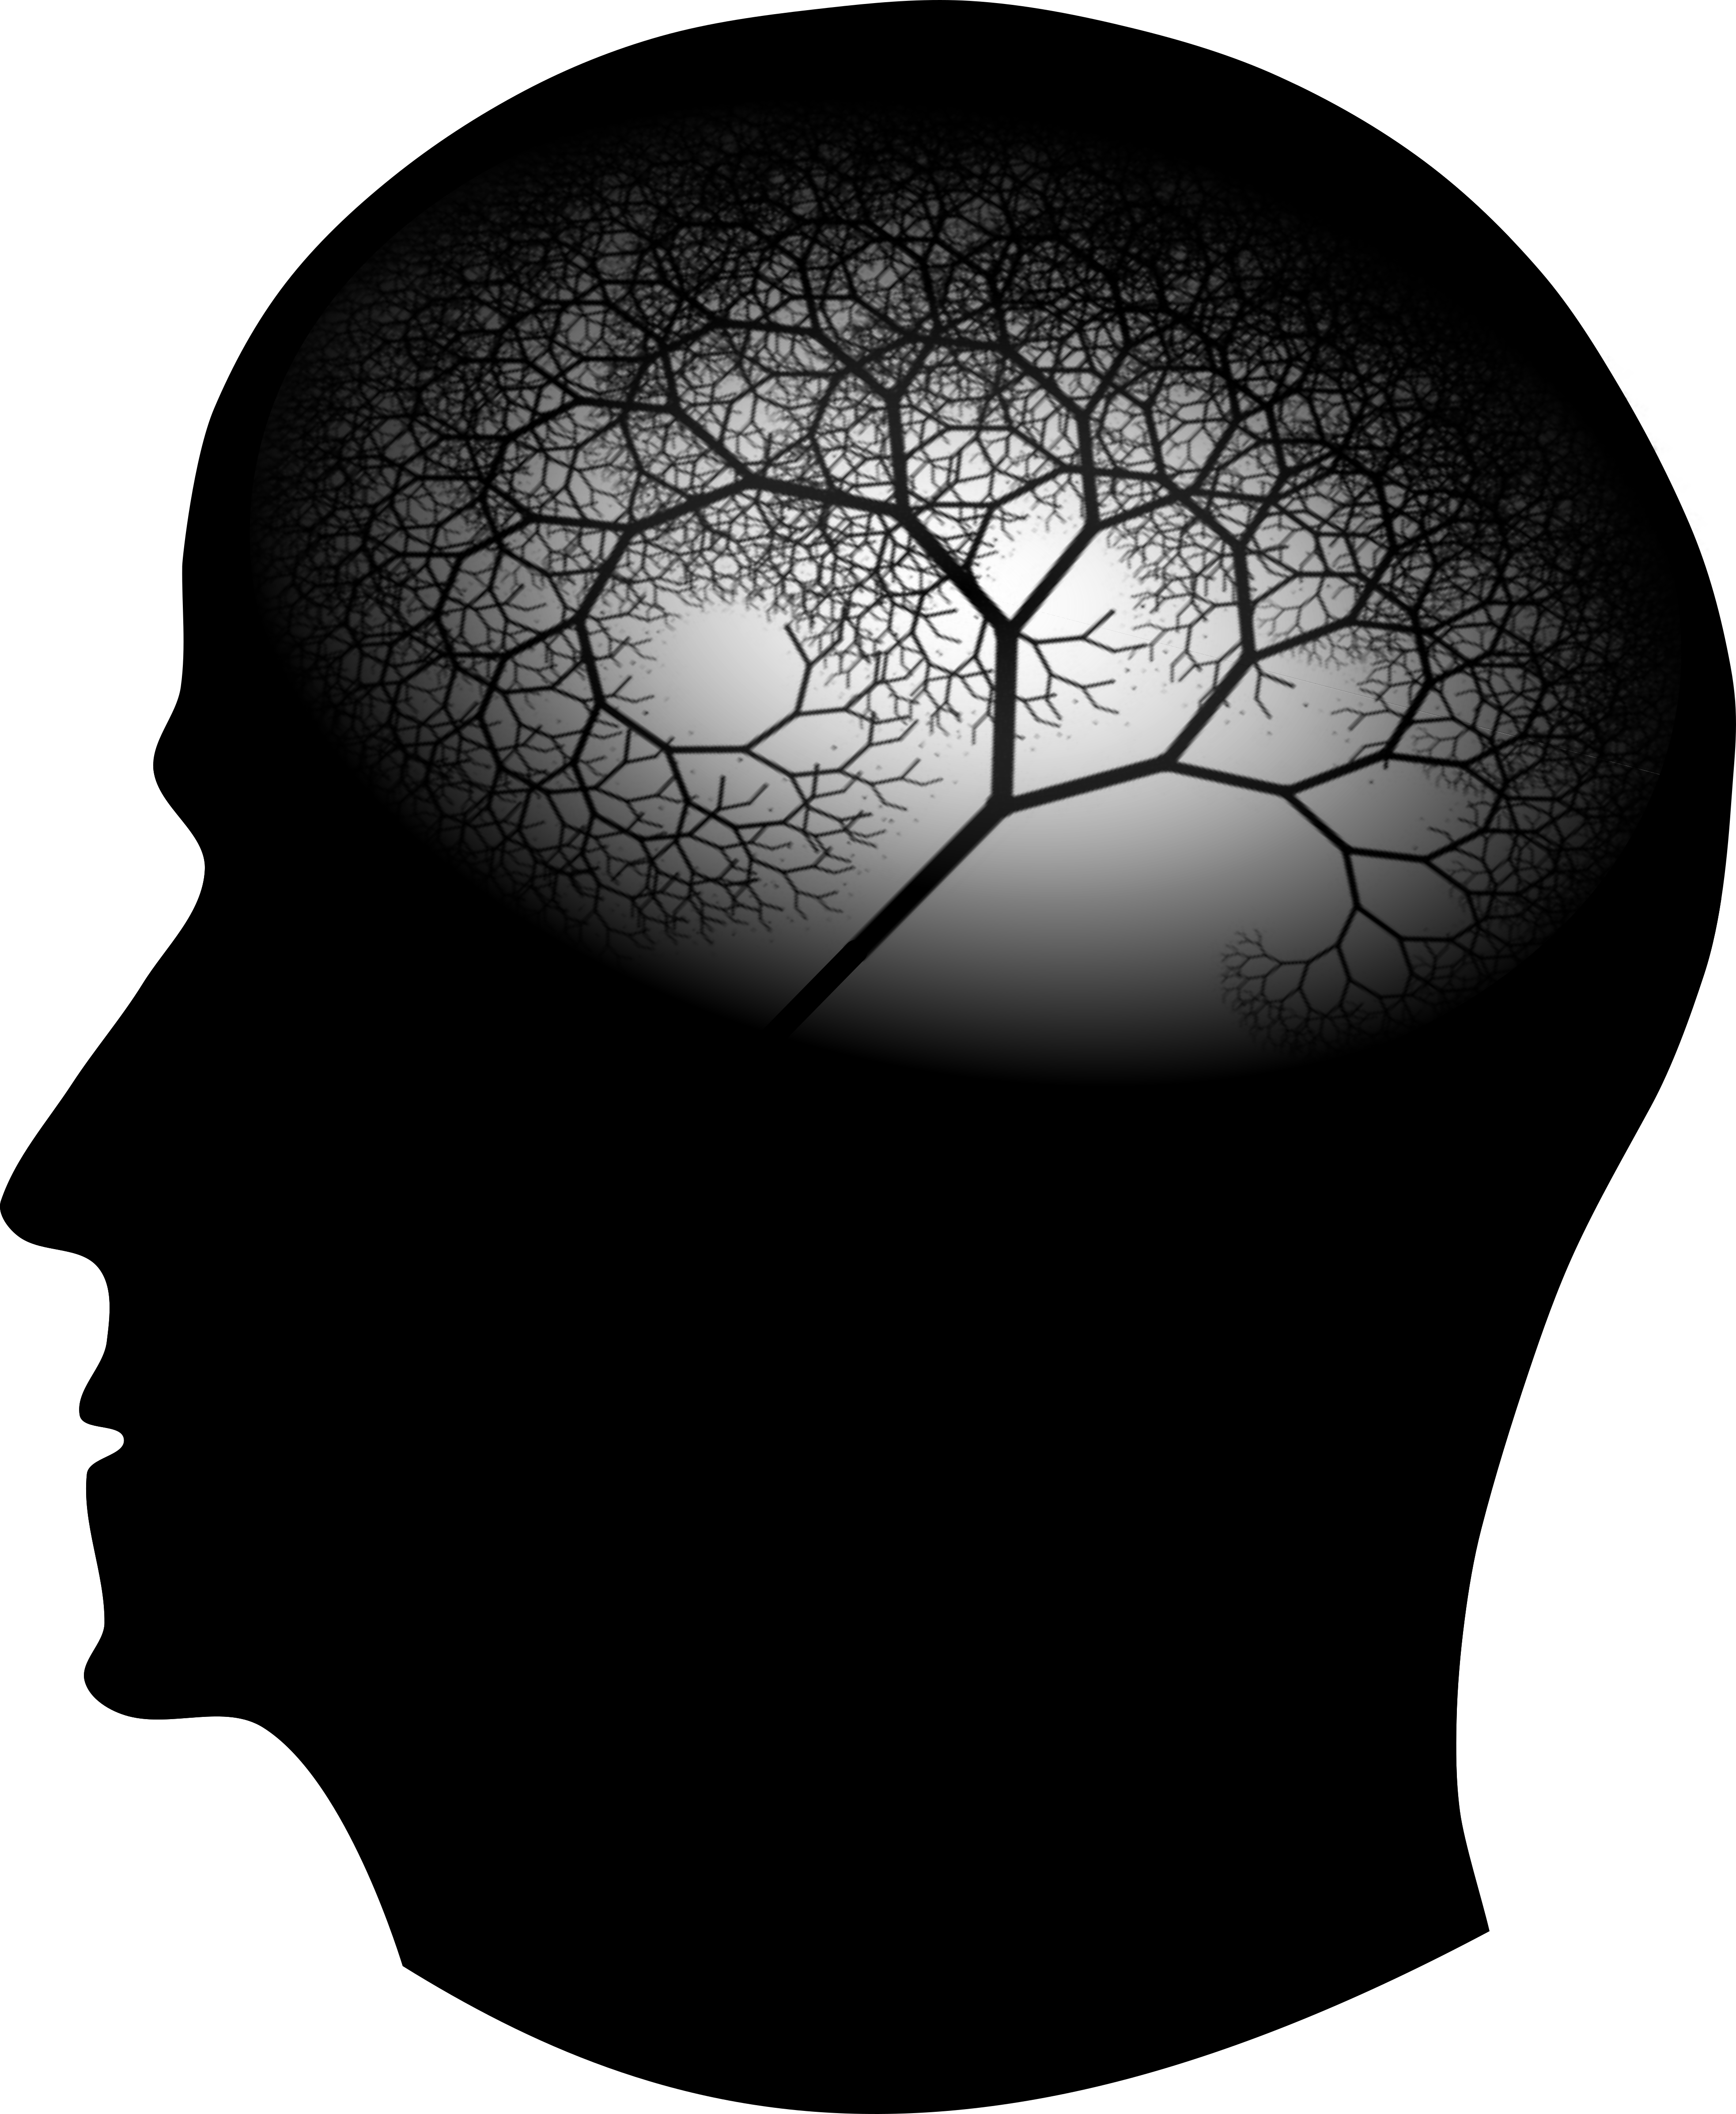
\includegraphics[width = 0.7\textwidth]{frase.png} 
\end{figure*}

\newpage

\setcounter{page}{1}
\pagenumbering{arabic}

%%%%%%%%%%%%%%%%%%%%%%%%%%%%%%%%%%%%%%%%%%%%%%%%%%%%%%%%%%%%%%%%%%%%%%%%%%%%%%%%%%%%%%%%%%%%%%%%%%%
%%%%%%%%%%%%%%%%%%%%%%%%%%%%%%%%%%%%%%%%%%%%%%%%%%%%%%%%%%%%%%%%%%%%%%%%%%%%%%%%%%%%%%%%%%%%%%%%%%%
%%%%%%%%%%%%%%%%%%%%%%%%%%%%%%%%%%%%%%%%%%%%%%%%%%%%%%%%%%%%%%%%%%%%%%%%%%%%%%%%%%%%%%%%%%%%%%%%%%%

\pagestyle{fancy}
%    \fancyhf{} 
    \fancyhead[LO]{\sectionmark}
    \fancyhead[RE]{\chaptermark}
    \fancyfoot[CE,CO]{}
    \fancyfoot[LE,RO]{\thepage}
    \renewcommand{\headrulewidth}{1.5pt}

%%%%%%%%%%%%%%%%%%%%%%%%%%%%%%%%%%%%%%%%%%%%%%%%%%%%%%%%%%%%%%%%%%%%%%%%%%%%%%%%%%%%%%%%%%%%%%%%%%%
%%%%%%%%%%%%%%%%%%%%%%%%%%%%%%%%%%%%%%%%%%%%%%%%%%%%%%%%%%%%%%%%%%%%%%%%%%%%%%%%%%%%%%%%%%%%%%%%%%%
%%%%%%%%%%%%%%%%%%%%%%%%%%%%%%%%%%%%%%%%%%%%%%%%%%%%%%%%%%%%%%%%%%%%%%%%%%%%%%%%%%%%%%%%%%%%%%%%%%%
%%%%%%%%%%%%%%%%%%%%%%%%%%%%%%%%%%%%%%%%%%%%%%%%%%%%%%%%%%%%%%%%%%%%%%%%%%%%%%%%%%%%%%%%%%%%%%%%%%%

\chapter*{Introducción}
\addcontentsline{toc}{chapter}{Introducción}

Gracias a los avances médicos del último siglo se han incrementado tanto la esperanza como la calidad de vida. 
%
Desafortunadamente, también ha aumentado la presencia de enfermedades no-transmisibles asociadas con la edad. 
%
En México el sector de la población con más de 60 años de edad (considerados en alto riesgo para este tipo de enfermedades) contempló a 10 millones de personas en 2010, y en 2015 dicha cifra creció a 12 millones \cite{Censo10,Intercensal15}.
%
En este trabajo se destaca la demencia entre las enfermedades asociadas con la edad.

La demencia consiste en el desarrollo de deficiencias cognoscitivas (especialmente en atención y memoria) suficientemente graves como para interferir en las actividades del individuo.
%
Hasta el momento, se considera que la demencia es irreversible, y no se han identificado curas \cite{PlanAlzheimer04}, debido a lo cual ha surgido un gran interés en definir y diagnosticar sus etapas tempranas.
%
El deterioro cognitivo leve (DCL), una etapa temprana de la demencia, se entiende como el desarrollo de deficiencias cognoscitivas \textit{objetivas} que no son lo suficientemente graves para calificarse como demencia.

Existen varios métodos para detectar el DCL, como la autopercepción por parte del paciente, análisis genéticos, químicos o de imagenología cerebral.
%
En este trabajo se destaca la polisomnografía (PSG), una técnica que consiste en el registro conjunto de varias señales electrofisiológicas durante el sueño.
%
De manera concreta, será analizada una PSG compuesta por registros de electroencefalografía (EEG), electrooculografía (EOG) y electromiografía (EMG), para medir actividad eléctrica cerebral, tono muscular y movimientos oculares, respectivamente.
%
Se decidió usar la PSG porque es una técnica relativamente barata y no invasiva --en relación al tipo de información que se obtiene--, y en la literatura hay una gran cantidad de reportes sobre marcadores para el DCL usando la EEG.

Se han encontrado, por ejemplo, asociaciones entre el DCL en adultos mayores con la \textit{presencia} de algunos tipos de ondas cerebrales \cite{babiloni13,prichep06,prichep94}.
%
Conviene destacar que algunos reportes indican que los mejores predictores del DCL son los obtenidos durante el sueño (incluso sólo el EEG) en comparación con los obtenidos durante la vigilia \cite{Brayet16}.

%%%%%%%%%%%%%%%%%%%%%%%%%%%%%%%%%%%%%%%%%%%%%%%%%%%%%%%%%%%%%%%%%%%%%%%%%%%%%%%%%%%%%%%%%%%%%%%%%%%
%%%%%%%%%%%%%%%%%%%%%%%%%%%%%%%%%%%%%%%%%%%%%%%%%%%%%%%%%%%%%%%%%%%%%%%%%%%%%%%%%%%%%%%%%%%%%%%%%%%

\section*{Antecedentes}
\addcontentsline{toc}{section}{Antecedentes}

Se considera que la técnica de EEG fue inventada en la década de 1920 por el fisiólogo Hans Berger, quien descubrió que ésta es \textit{sensible} a cambios en la actividad mental como la atención sostenida o el parpadeo voluntario.
%
Desde entonces se estableció que hay una \textit{conexión} entre el funcionamiento de la mente y los fenómenos eléctricos en el cerebro.
%
%Después de casi un siglo, se ha llegado a aceptar que dicha asociación es más bien complicada.

Los fenómenos eléctricos en el cerebro que dan origen al EEG se consideran comprendidos en sus \textit{niveles de organización} más básicos: cada neurona genera un potencial eléctrico estable a través de su membrana celular, debido al intercambio de iones con el medio extracelular.
%
Las perturbaciones en estos \textit{potenciales de membrana} se trasmiten a través de la misma, e inducen perturbaciones similares en neuronas cercanas; la morfología de las neuronas permite que formen \textit{redes} para la transmisión de impulsos eléctricos, las cuales se extienden por todo el sistema nervioso.
%
%Estas formas de organización ha atrapado la atención de una gran cantidad de personas, sobre cómo funciona este sistema o cómo deja de funcionar.
%

A partir de este mecanismo para la transmisión de impulsos eléctricos, sin embargo, no es muy claro cómo funciona el sistema nervioso central como un todo --o cómo deja de funcionar, como en el caso del DCL.
%
La existencia de múltiples niveles de organización en la actividad cerebral la han colocado como un \textit{paradigma} de complejidad.
%; en otras palabras la actividad cerebral es más que un ejemplo en teoría de la complejidad, es un fenómeno alrededor del cual se construye gran parte la teoría)
%Por complejidad se entiende las propiedades de algunos sistemas que dependen de la \textit{escala}, así como los estados de agregación (sólido, 
En este contexto se entiende a la complejidad no como complicación, sino como la presencia de características \textit{emergentes}, es decir, que están presentes en un sistema pero no en sus componentes: una neurona individual no tiene --cualitativamente-- el mismo comportamiento eléctrico que todo el cerebro \cite{Werner09}.
%
La complejidad puede describirse informalmente con la frase ``el todo es más que [simplemente] la suma de las partes", entendiendo que la organización es parte de un sistema.
% es una parte fundamental del mismo. %[?? citar articulo dfa vs patrones locales]

%Por un lado el EEG es en parte un fenómeno eléctrico, tradicionalmente se le describe en términos de ondas y frecuencias, en ocasiones como un sistema dinámico.
%%
%Paralelamente el EEG es un fenómeno biológico, de modo que se le atribuyen características estocásticas pero --de alguna forma-- organizadas.
%
En su libro \textit{``Cybernetics or Control and Communication in the Animal and the Machine"}, el matemático Norbert Wiener 
%comenta la posibilidad de que la actividad cerebral tenga un poco de ambas características, lo cual no lo excusa de ser estudiado formalmente (es decir, sin vageudad) como un sistema \cite{wiener61} cap11.
propuso que 
%es --en principio-- posible estudiar al cerebro usando medidas propias de la teoría de la información; como 
debido por la gran complejidad de la actividad cerebral, el comportamiento del EEG roza la aleatoriedad; entonces es posible estudiar estos fenómenos usando herramientas de estadística, ignorando parcialmente los procesos físicos y biológicos subyacentes
\cite{wiener61}.
%
Con base a tal comentario, surge históricamente la pregunta sobre hasta qué punto es posible es posible modelar efectivamente al EEG como señales aleatorias con propiedades \textit{simples}.
%se investigó hicieron múltiples esfuerzos por determinar hasta qué punto es posible usar de manera efectiva la simplificación estadística del EEG.
% era posible aprovechar dicho efecto efectivamente posible modelar al EEG de forma independiente a su complejidad nata.
%
Por ejemplo, pueden mencionarse varios trabajos pioneros donde se investiga si los registros de EEG siguen una distribución normal, si son estacionarios, y si su espectro de potencias es \textit{estable} en el tiempo
\cite{Kawabata73,McEwen75,Sugimoto78,Cohen77};
%%En los trabajos pioneros de Kawabata \cite{Kawabata73}, McEwen \cite{McEwen75}, Sugimoto \cite{Sugimoto78}, Cohen \cite{Cohen77}, 
en dichos trabajos se demuestra experimentalmente que el EEG puede considerarse estacionario si se usan segmentos de hasta 20 segundos, e incluso se sugiere que esta cantidad puede cambiar para personas con alguna daño neuronal.
% en el EEG de personas sanas y con deterioro cognitivo.

Es sumamente interesante el contraste entre la complejidad \textit{por naturaleza} del EEG, y la posibilidad de extraer segmentos cuyo comportamiento es relativamente simple.
%
Se ha propuesto que esta característica corresponde a la \textit{orquestación} de múltiples estados de actividad, que se alternan en intervalos irregulares de tiempo logrando una gran heterogeneidad global \cite{kaplan2000application}.
%
%una formalización de estas características es la \textbf{estacionariedad local} por Dahlhaus \cite{Dahlhaus97}.
En el caso de la estacionariedad, se usará la formalización para este comportamiento descrita por Dahlhaus, referida como \underline{estacionariedad local} \cite{Dahlhaus97}.

%El estudio de la estacionariedad ha sido usado por varios autores para detectar estos \textit{cambios estructurales} en diferentes procesos, por ejemplo Kaplan para segmentar el EEG [??citar kaplan lbro] o Nason para detectar ondas sísmicas \cite{Nason13}.
%%
%Sin embargo, su detección formal está en desuso dentro de los análisis de rutina bajo el supuesto

Respecto al supuesto de estacionariedad local en el EEG, la verificación formal de estacionariedad ha caído en desuso; en cambio, se suelen usar fragmentos de EEG \textit{suficientemente pequeños} para poder suponer estacionariedad \cite{Kaiser00}. % [citar eeg milestones].
%
Las pruebas de estacionariedad han sido útiles, por ejemplo
%Sin embargo, se ha demostrado que la estacionariedad local puede ser usada, por ejemplo,
%Sin embargo, el concepto como tal es usado, por ejemplo, 
para segmentar de forma \textit{fisiológicamente relevante} registros de EEG \cite{Kaplan99} y de magnetoencefalografía\footnote{La técnica de magnetoencefalografía (MEG) consiste en el registro de actividad eléctrica del cerebro, a través de perturbaciones en campos magnéticos artificiales.} \cite{lazyref1}.

Bajo el supuesto de estacionariedad local, en el presente trabajo se explora la hipótesis en que el DCL afecte a la organización de la actividad cerebral.
%
De manera concreta se realizaron análisis sobre el grado de estacionariedad de segmentos de PSG para comprobar si hay cambios en los resultados entre individuos con y sin DCL.
% algún tipo de organización asociada a la estacionariedad, y se espera que esta organización cambie de alguna forma en individuos con DCL; 
%Se estudia el EEG durante el sueño porque, como se señaló antes, es una condición mental dirigida.
%
Previamente, se han mostrado resultados que sugieren es posible observar tales cambios
%ya se habian presentado resultados previos
%En un estudio reciente, EEG de una noche polisomnografía de personas mayores con y sin deterioro cognitivo según las evaluaciones con el Neuropsi analizó el porcentaje de estacionariedad.  En sueño MOR el porcentaje fue menor que el del sueño NMOR y la vigilia, se obtuvo estacionariedad  como un índice para comparar NMOR versus sueño MOR en ambos grupos 
%\cite{Rosales-Lagarde17}.

Cabe mencionar que para detectar el grado de estacionariedad se ha usado la prueba
% para detectar estacionariedad
%Para detectar la estacionariedad se ha usado la prueba propuesta 
descrita
por Priestley y Subba Rao \cite{Priestley69} ya que se ha señalado como una de las más rápidas hasta la fecha \cite{Nason13}, y porque puede ser interpretada de forma relativamente sencilla en términos de un espectro de potencias cambiante en el tiempo. 
%
Esta última característica es deseable en vista a la gran literatura que existe sobre espectros de potencia para el EEG.

%En el presente trabajo se opta por interpretar (como sinónimo informal para \textit{`modelar'}) a los registros de EEG como procesos estocásticos cuyo espectro de potencias es relevante; naturalmente, ambos términos serán definidos con detalle en el texto.

%La actividad eeeg representa unn paradigma de complejidad, que no es sinónimo de complicadion sino de actividad emergente.
%como los estados de agregacion de la materia.
%el todo es mas que la suma de las partes
%[?? citar articulo dfa vs patrones locales]

%la estacionariedad local y dahlhaus.

%El enfoque de estacionariedad, desde la perspectiva del espectro, ha sido tomado por varios autores. Por ejemplo Kaplan, quien lo usa para definir fragmentos cuyo espectro de potencias es omogeneo. 
%
%Los fragmentos son ni portantes porque

%la clase cohen y diferentes espectros cambiantes en el teimpo

%Se usa la prueba propuesta por Priestley y Subba Rao.
%Por ejemplo Nason, quien usa la estacionairedad en vulcanologia para detectar cosas. La prueba de PSR es una de las mas rapidas porque es nlog(n)

%tiempo, fft y computadoras: tiene sentido usar pruebas viejas y raras

%En 2016 Vázquez-Tagle y colaboradores estudiaron el PDCL en adultos mayores del estado de Hidalgo con el método no lineal del Análisis de Fluctuaciones sin Tendencia (DFA, por sus siglas en inglés), encontrando efectivamente que los sujetos con PDCL presentan mayor ruido browniano en varias regiones en comparación con los pacientes sin PDCL\cite{VazquezTagle16}.

En el presente trabajo se busca desarrollar un método para determinar el DCL con base en registros de PSG en adultos mayores, como un marcador que respalde los resultados de pruebas neuropsicológicas.
%
Se mantiene presente que el deterioro cognitivo (más allá del DCL) no puede reducirse exclusivamente a tales mediciones, y que las conclusiones obtenidas 
%usando registros de señales electrofisiológicas 
deben ser contrastadas con resultados de análisis complementarios.

%%%%%%%%%%%%%%%%%%%%%%%%%%%%%%%%%%%%%%%%%%%%%%%%%%%%%%%%%%%%%%%%%%%%%%%%%%%%%%%%%%%%%%%%%%%%%%%%%%%
%%%%%%%%%%%%%%%%%%%%%%%%%%%%%%%%%%%%%%%%%%%%%%%%%%%%%%%%%%%%%%%%%%%%%%%%%%%%%%%%%%%%%%%%%%%%%%%%%%%

\section*{Pregunta de investigación y objetivos}
\addcontentsline{toc}{section}{Pregunta de investigación y objetivos}

Los registros de PSG en adultos mayores, modelados como procesos estocásticos, ¿pueden considerarse como débilmente estacionarios?
%
¿Dicha caracterización es afectada si el individuo presenta probable DCL o PDCL?

%%%%%%%%%%%%%%%%%%%%%%%%%%%%%%%%%%%%%%%%%%%%%%%%%%%%%%%%%%%%%%%%%%%%%%%%%%%%%%%%%%%%%%%%%%%%%%%%%%%

\subsection*{Objetivos}

Estudiar pruebas estadísticas para detectar si una realización dada proviene de un proceso estocástico débilmente estacionario.
%
Usar tales pruebas sobre registros de PSG en adultos mayores con y sin PDCL; bajo el supuesto de estacionariedad local, revisar qué factores podrían influir en los resultados obtenidos.
%
Investigar si hay una relación entre la presencia de PDCL y la clasificación de los proceso estocásticos referidos como débilmente estacionarios.


\section*{Acerca de la estructura del texto}
%\addcontentsline{toc}{section}{Sobre la estructura del texto}

Debido al enfoque aplicado del presente trabajo, esta porción del texto fue estructurada pensando en dos tipos de lectores: por un lado aquellos interesados principalmente en los objetos matemáticos involucrados y sus conexiones, y por otro lado quienes ven los mismos como herramienta y esperan entenderlos mejor.
%
Los temas fueron ordenados pensando en el primer tipo de lector.
%
Para el segundo tipo de lector, se ha preparado en la figura \ref{intro:estructura} un \textit{mapa} del texto, pero principalmente de los temas sobre matemáticas.

En el primer capítulo se abordan varios temas preliminares sin lujo de detalles, con la finalidad de presentar un texto autocontenido;
%
la finalidad del capítulo es definir formalmente los procesos estocásticos, espacios de Hilbert y estimadores.

En el segundo capítulo se definen los procesos estocásticos débilmente estacionarios, al conjunto de éstos se les da estructura de espacio de Hilbert, y finalmente se usa dicha estructura para definir el espectro de potencias como una generalización de la transformada de Fourier.
%
Una porción importante del capítulo trata sobre la estimación efectiva del espectro de potencias a partir de observaciones dadas de un proceso estocástico.

En el tercer capítulo se define el \textit{espectro evolutivo}, una generalización del espectro de potencias para una familia de procesos que no son débilmente estacionarios.
%
Al final se expone una aplicación aparente menor del espectro evolutivo, pero que es fundamental para el resto del presente trabajo: la prueba de Priestley Subba-Rao. 
%
Esta prueba verifica --como prueba de hipótesis-- si el espectro evolutivo de un proceso puede reducirse a un espectro de potencias; en otras palabras, si un proceso es débilmente estacionario.

En el cuarto capítulo se presentan conceptos de índole \textit{fisiológica}: psicología, psicometría, electrofisiología.
%
El objetivo del capítulo es describir el DCL y cómo se detecta, describir qué es el sueño y como se analiza (en este caso a partir de la polisomnografía), y mencionar la relación entre el sueño y el DCL.

En el capítulo quinto se describe cómo se utilizó la prueba de estacionariedad débil para estudiar los registros de polisomnografía.
%
En el capítulo sexto se discuten los resultados obtenidos, y se concluye que la técnica utilizada es un marcador diagnóstico para el DCL; se reportan algunos hallazgos incidentales.

\begin{figure}
\centering
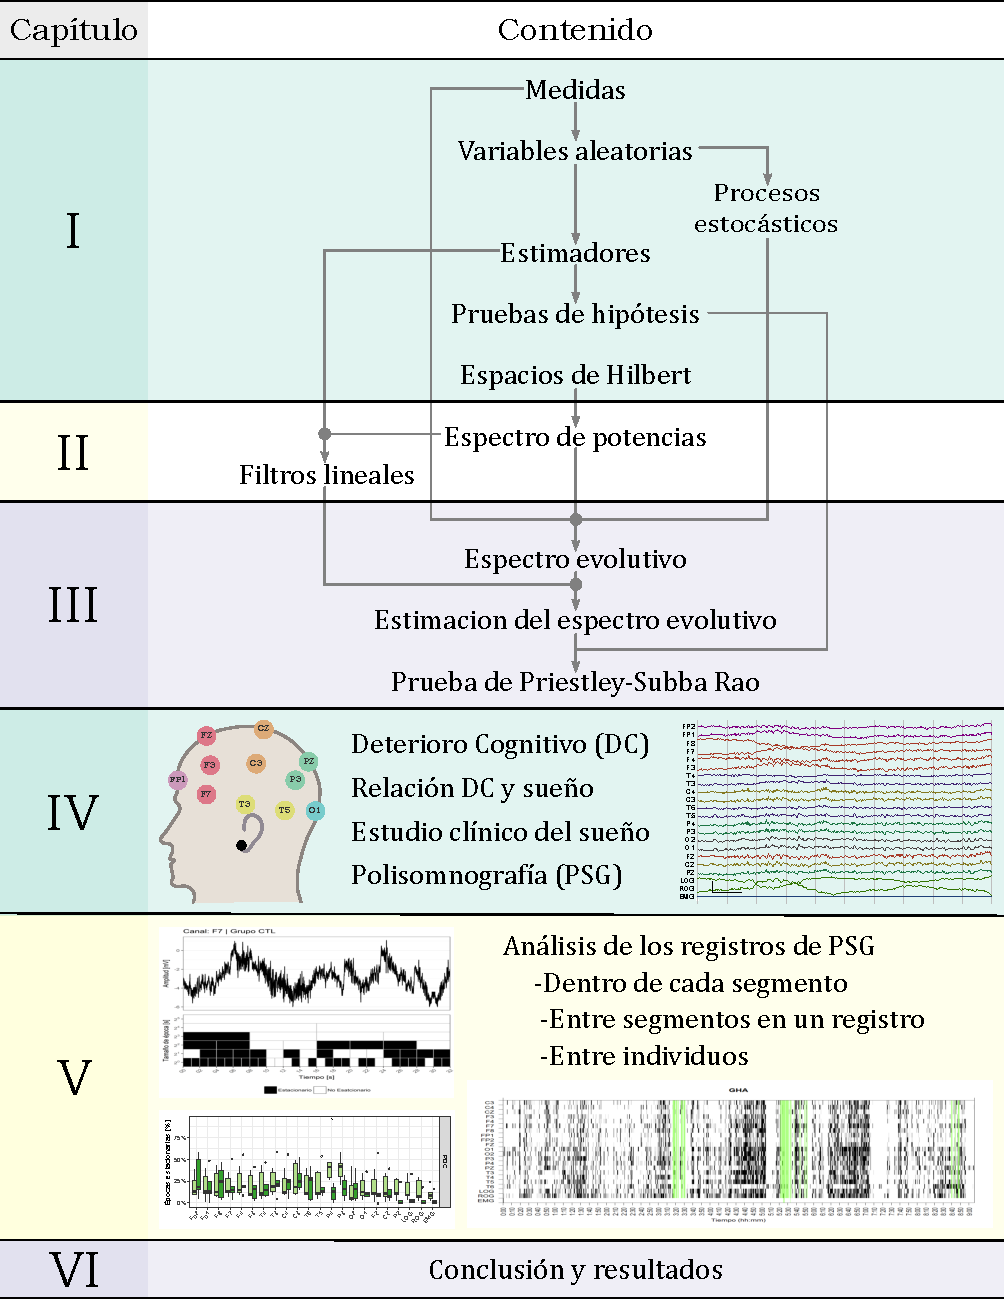
\includegraphics[width=.9\textwidth]{./estructura_texto_v2.pdf}
\caption[Estructura de la tesis]{Se ilustra gráficamente las \textit{dependencias} respecto a los tópicos de matemáticas, es decir, los temas que deben discutirse antes que otros. El resto del texto (incluyendo los tópicos de fisiología) son expuestos de forma más \textit{secuencial}, por lo que no se consideró necesario ilustrar sus dependencias.}
\label{intro:estructura}
\end{figure}

%%%%%%%%%%%%%%%%%%%%%%%%%%%%%%%%%%%%%%%%%%%%%%%%%%%%%%%%%%%%%%%%%%%%%%%%%%%%%%%%%%%%%%%%%%%%%%%%%%%
%%%%%%%%%%%%%%%%%%%%%%%%%%%%%%%%%%%%%%%%%%%%%%%%%%%%%%%%%%%%%%%%%%%%%%%%%%%%%%%%%%%%%%%%%%%%%%%%%%%
%%%%%%%%%%%%%%%%%%%%%%%%%%%%%%%%%%%%%%%%%%%%%%%%%%%%%%%%%%%%%%%%%%%%%%%%%%%%%%%%%%%%%%%%%%%%%%%%%%%
%%%%%%%%%%%%%%%%%%%%%%%%%%%%%%%%%%%%%%%%%%%%%%%%%%%%%%%%%%%%%%%%%%%%%%%%%%%%%%%%%%%%%%%%%%%%%%%%%%%

%%%%%%%%%%%%%%%%%%%%%%%%%%%%%%%%%%%%%%%%%%%%%%%%%%%%%%%%%%%%%%%%%%%%%%%%%%%%%%%%%%%%%%%%%%%%%%%%%%%
%%%%%%%%%%%%%%%%%%%%%%%%%%%%%%%%%%%%%%%%%%%%%%%%%%%%%%%%%%%%%%%%%%%%%%%%%%%%%%%%%%%%%%%%%%%%%%%%%%%
%%%%%%%%%%%%%%%%%%%%%%%%%%%%%%%%%%%%%%%%%%%%%%%%%%%%%%%%%%%%%%%%%%%%%%%%%%%%%%%%%%%%%%%%%%%%%%%%%%%

\chapter{Preliminares}

Este capítulo se incluye con el objetivo de lograr un texto autocontenido y accesible, para lo cual se expone una serie de temas que en lo posterior serán considerados como \textit{conocidos}.
%
Dentro del contexto del presente trabajo, la lectura de este capítulo es opcional, para lo cual se recomienda revisar el diagrama de relaciones entre temas (cuadro \ref{intro:estructura}) como guía de lectura.
%
La secuencia de lectura sugerida por el autor es, naturalmente, según se ha ordenado el texto de principio a fin.

Con la intención de no hacer el presente texto innecesariamente extenso, los temas del presente capítulo se exponen sin muchos detalles; se omiten comentarios importantes y demostraciones de teoremas fuertes, pero sólo en caso de que no \textit{impacten} de manera directa a los resultados centrales del presente trabajo.
%
Esta falla planificada es \textit{compensada} citando material donde el lector puede encontrar dichos faltantes.
%
Cabe destacar que los temas \textit{centrales} en el presente texto se distribuyen entre los capítulos 2 y 3.

De manera general, el lector interesado en mayores detalles sobre teoría de la medida, probabilidad y estadística puede referirse a los libros \textit{``Probability for Statisticians"} por Galen R. Shorack \cite{probabilidad_shorack}, y \textit{``Statistical Theory"} por Bernard W. Lindgren \cite{estadistica_lindgren}.
%
Así mismo, en el contexto de procesos estocásticos, es recomendable la exposición sobre espacios de Hilbert en el libro \textit{``Stationary Stochastic Processes: Theory and Applications"} por Georg Lindgren \cite{estacionariedad_lindgren}.

%%%%%%%%%%%%%%%%%%%%%%%%%%%%%%%%%%%%%%%%%%%%%%%%%%%%%%%%%%%%%%%%%%%%%%%%%%%%%%%%%%%%%%%%%%%%%%%%%%%
%%%%%%%%%%%%%%%%%%%%%%%%%%%%%%%%%%%%%%%%%%%%%%%%%%%%%%%%%%%%%%%%%%%%%%%%%%%%%%%%%%%%%%%%%%%%%%%%%%%

\section{Medidas}

\begin{definicion}%[$\boldsymbol{\sigma}$-álgebra]
Sea $\Omega$ un conjunto y sea $\mathcal{U}$ una familia de subconjuntos de $\Omega$. Se dice que $\mathcal{U}$ es una \textbf{$\boldsymbol{\sigma}$-álgebra} si cumple
\begin{itemize}
\item $\Omega \in \mathcal{U}$
\item $A \in \mathcal{U} \Rightarrow A^{C} \in \mathcal{U}$
\item 
$ \displaystyle \{ A_n \}_{n\in \mathbb{N}} \subseteq \mathcal{U} 
\Rightarrow \cup_{n\in \mathbb{N}} A_n \in \mathcal{U}$
\end{itemize}
Donde $A^{C}$ es el complemento de $A$ en $U$. Los elementos de $\mathcal{U}$ se denominan \textbf{conjuntos medibles}. 
\end{definicion}

\begin{definicion}
Sea $\Omega$ un conjunto y $\mathcal{A} \subseteq \Omega$ una familia de subconjuntos. Se define a $\sigma(\mathcal{A})$, la $\sigma$-álgebra generada por $\mathcal{A}$, como la intersección de todas las $\sigma$-álgebras que contienen a $\mathcal{A}$.
\end{definicion}

\begin{ejemplo}
En el contexto de la probabilidad, es particularmente importante la \underline{$\sigma$-álgebra de Borel}, $\mathcal{B}$, definida como
\begin{equation}
\mathcal{B} := \sigma\left( \left\{ \left( -\infty , a \right] \subset \R \talque a\in \R \right\} \right)
\end{equation}

En general pueden definirse $\sigma$-álgebras similares de forma sencilla para algún subconjunto arbitrario $A \subset \R$, como
\begin{equation}
\mathcal{B}_A := \sigma\left( \left\{ \left( -\infty , a \right] \cap A \subset \R \talque a\in \R \right\} \right)
\end{equation}
\end{ejemplo}

\begin{definicion}
Sea $\Omega$ un conjunto y $\mathcal{U}$ una $\sigma$-álgebra definida en $\Omega$. El par $(\Omega,\mathcal{U})$ será referido como \textbf{espacio de medida}. Por nomenclatura, $\Omega$ es referido como \textit{espacio muestral} y $\mathcal{U}$ como \textit{$\sigma$-álgebra de sucesos}.
\end{definicion}

\begin{definicion}%[Medida]
Sea $(\Omega, \mathcal{U})$ un espacio de medida. Se dice que una función $\mu : \mathcal{U} \rightarrow \R_+$ es una \textbf{medida} si cumple que
\begin{itemize}
\item $\mu(\emptyset) = 0$
\item Si $\{ A_n \}_{n\in \mathbb{N}} \subseteq \mathcal{U}$ son tales que $A_n \cap A_m = \emptyset \Leftrightarrow m\neq n$, entonces 
\begin{equation}
\mu\left( \bigcup_{n\in \mathbb{N}} A_n \right) = \sum_{n\in \mathbb{N}} \mu(A_n)
\end{equation}
\end{itemize}
Donde $\R_+ = \left\{ x\in \R \talque 0 \leq x \right\} \cup \{ \infty \}$ y $\emptyset$ es el conjunto vacío. La terna $(\Omega,\mathcal{U},\mu)$ será referida como \textbf{espacio de medida}.
\label{medida}
\end{definicion}

%\begin{definicion}%[Medida $\boldsymbol{\sigma}$-finita]
%Sea $(\Omega,\mathcal{U},\mu)$ un espacio de medida. Se dice que $\mu$ es \textbf{$\boldsymbol{\sigma}$-finita} si existen una familia de conjuntos medibles $\{ A_n \}_{n\in \mathbb{N}}$ tales que
%\begin{itemize}
%\item $\mu\left( A_n \right) < \infty$
%\item $ \bigcup_{n\in \mathbb{N}} A_n = \Omega$
%\end{itemize}
%\end{definicion}

\begin{ejemplo}
Considérese el espacio medible $(\R, \mathcal{B})$, con $\mathcal{B}$ la $\sigma$-álgebra de Borel. Se define la \ul{medida de Lebesgue}, $\mu_L$, la medida en el espacio mencionado que satisface 
\begin{equation}
\mu_L([a,b]) = b-a
\end{equation}
para cualesquiera $a,b \in \R$ con $a<b$. Por simplicidad, en lo posterior se dará por entendido que el espacio de medida $(\R, \mathcal{B},\mu_L)$ es \textit{usual} siempre que se hable de medidas en $\R$ o alguno de sus subconjuntos.
\end{ejemplo}

\begin{ejemplo}
Considérese el espacio medible $(\R, \mathcal{B})$, con $\mathcal{B}$ la $\sigma$-álgebra de Borel. Se define la \ul{medida discreta}, $\mu_D$, como
\begin{equation}
\mu_D(A) = \sigma_{n \in A \cup \N} 1
\end{equation}
\end{ejemplo}

%%%%%%%%%%%%%%%%%%%%%%%%%%%%%%%%%%%%%%%%%%%%%%%%%%%%%%%%%%%%%%%%%%%%%%%%%%%%%%%%%%%%%%%%%%%%%%%%%%%

\subsection{Integración en espacios medibles}

\begin{definicion}
Sea $(\Omega_1, \mathcal{U}_1)$ y $(\Omega_2, \mathcal{U}_2)$ dos espacios de medida. Se dice que una función $f:\Omega_1\rightarrow\Omega_2$ es una \textbf{función medible} si cumple que
\begin{equation}
U \in \mathcal{U}_2 \Rightarrow f^{-1}(U) \in \mathcal{U}_1 
\end{equation}
donde $f^{-1}(U) = \left\{ u\in \Omega_1 \talque f(u) \in U \right\}$.
\end{definicion}

\begin{definicion}
Sea $(\Omega, \mathcal{U})$ un espacio de medida, sea $C \in \mathcal{U}$ un conjunto medible arbitrario, sea $n\in \N$. Una \textbf{partición} de $C$ es una familia de conjuntos $\{E_1, E_2, \dots, E_n\} \subseteq\mathcal{U}$ que satisface las siguientes condiciones:
\begin{itemize}
\item $E_i \cap E_j = \emptyset \Leftarrow i\neq j $
\item $\cup_{i=1}^{N}  E_i = C $
\end{itemize}
\end{definicion}

\begin{definicion}
Sea $(\Omega, \mathcal{U}, \mu)$ un espacio de medida y sea $f:\Omega \rightarrow \R_+$ una función medible. Sea $A\in \mathcal{U}$ un conjunto arbitrario, y sea $\mathcal{C}_A \subset \mathcal{U}$ el conjunto de las particiones de $A$.
Se define la \textbf{integral de $\boldsymbol{f}$ respecto a $\boldsymbol{\mu}$ en $\boldsymbol{A}$} como
\begin{equation}
\int_A f(x) \mu(x) := \sup_{\mathcal{C}_A} \left[ \sum_{i=1}^{N} f_i f(\lambda) \mu(E_i) \right]
\end{equation}
donde $\{ E_1, E_2, \dots, E_N \}$ es una partición arbitraria de $A$ y $f_i = \inf_{t \in E_i} f(t)$.
\label{def:lazy1}
\end{definicion}

\begin{definicion}
Sea $(\Omega, \mathcal{U}, \mu)$ un espacio de medida y sea $f:\Omega \rightarrow \R_+$ una función medible. Se definen las funciones $f^{+}$ y $f^{-}$ como
\begin{align*}
f^{+}(x) &= \max (f(x), 0 ) \\
f^{-}(x) &= -\min (f(x), 0 )
\end{align*}
Se dice que $f$ es \textbf{integrable en $\boldsymbol{A}$ respecto a $\boldsymbol{\mu}$} si cumple que $\int_A f^{+}(\lambda) d\mu(\lambda) < \infty$ y $\int_A f^{-}(\lambda) d\mu(\lambda) < \infty$; si así fuere, se define
\begin{equation}
\int_A f(\lambda) d\mu(\lambda) := \int_A f^{+}(\lambda) d\mu(\lambda) - \int_A f^{-}(\lambda) d\mu(\lambda)
\end{equation}
\label{def:lazy2}
\end{definicion}

\begin{proposicion}
Sea $(\Omega, \mathcal{U}, \mu)$ un espacio de medida, sean $f,g:\Omega \rightarrow \R_+$ funciones integrables en $A$ con respecto a $\mu$, y sean $\alpha, \beta \in \R$ arbitrarios. 
%
Se cumple que la función $[\alpha f + \beta g]$ es integrable en $A$ con respecto a $\mu$, y
\begin{equation}
\int_A \left[ \alpha f + \beta g \right] (\lambda) \mu(\lambda) = \alpha \int_A f(\lambda) \mu(\lambda) + \beta \int_A g(\lambda) \mu(\lambda)
\end{equation}
\end{proposicion}

\begin{proposicion}
Sea $(\Omega, \mathcal{U}, \mu)$ un espacio de medida y sea $f:\Omega \rightarrow \R_+$ una función medible. La función $\mu_f:\mathcal{U}\rightarrow\R_+$, definida como
\begin{equation}
\mu_f(A) := \int_A f(\lambda) \mu(\lambda)
\end{equation}
es una medida para el espacio medible $(\Omega, \mathcal{U})$. En tal caso, se dice que $\mu_f$ es la \textbf{medida inducida} por $f$.
\end{proposicion}
%\begin{proof}
%[?] Si se necesita, en la pagina 39 el manual
%\end{proof}

%\begin{proposicion}
%Sea $(\Omega, \mathcal{U}, \mu)$ un espacio de medida y sea $A\in \mathcal{U}$ arbitrario. Sean $f,g:\Omega \rightarrow \R_+$ una ???? función medible, y $\mu_f$ su medida inducida. Una función medible $g:$ es integrable en $A \in \mathcal{U}_2$ respecto a $\mu_f$ si y sólo si $g \circ f$ es integrable en $f^{-1}(A)$ respecto a $\mu$. En dado caso, se satisface que
%\begin{equation}
%\int_A g(\lambda) d\mu_f(\lambda) = \int_{f^{-1}(A)} g \circ f (\lambda) d\mu(\lambda)
%\end{equation}
%\end{proposicion}
%\begin{proof}
%asdasd [?] pagina 47 del manual
%\end{proof}

\begin{proposicion}
Sea $(\Omega, \mathcal{U}, \mu)$ un espacio de medida, sea $f:\Omega \rightarrow \R_+$ una función medible con $\mu_f$ su medida inducida, y sea $A\in \mathcal{U}$ arbitrario.
%
Si una función $g:\Omega \rightarrow \R_+$ es integrable en $A$ respecto a $\mu_f$, entonces se cumple que 
\begin{equation}
\int_A g(\lambda) d\mu_f(\lambda) = \int_{f^{-1}(A)} g(\lambda) f(\lambda) d\mu(\lambda)
\end{equation}

Como notación, este hecho será escrito como
\begin{equation}
d\mu_f(\bullet) = f(\bullet) d\mu(\bullet) 
\end{equation}
\label{lazy3}
\end{proposicion}
%\begin{proof}
%asdasd [?] pagina 47 del manual
%\end{proof}

%La notación anterior pude extenderse será usada para funciones reales.

%%%%%%%%%%%%%%%%%%%%%%%%%%%%%%%%%%%%%%%%%%%%%%%%%%%%%%%%%%%%%%%%%%%%%%%%%%%%%%%%%%%%%%%%%%%%%%%%%%%

\section{Variables aleatorias}

Si una medida $\mu$ es acotada en todo el espacio de eventos se dice que es una \textbf{medida finita}.% (no confundir con $\sigma$-finita). 
%
Una medida de probabilidad puede entenderse como un caso particular de medida finita sobre $\R$.

\begin{definicion}
El espacio de medida $(\Omega,\mathcal{U},P)$ se dice un \textbf{espacio de probabilidad} si satisface que $P(\Omega) = 1$.
\end{definicion}

%\begin{definicion}
%Sean $(\Omega_1,\mathcal{U}_1)$ y $(\Omega_2,\mathcal{U}_2)$ dos espacios medibles. Se dice que una función $f: \omega_1 \rightarrow \Omega_2$ es \textbf{medible} si para todo $A\in \mathcal{U}_2$
%$f^{-1}(A)\in\mathcal{U}$
%\end{definicion}

\begin{definicion}
Sea $(\Omega,\mathcal{U})$ un espacio medible y $(I,\mathcal{B}_I,P)$ un espacio de probabilidad. Una \textbf{variable aleatoria} es una función medible $X: \Omega \rightarrow \mathcal{B}_I$.
\label{lazy4}
\end{definicion}

\begin{definicion}
Una \textbf{variable aleatoria real} es un caso particular de variable aleatoria entre el espacio de medida $(\R,\mathcal{B},\mu_L)$ consigo mismo.
\end{definicion}

%Siendo $X$ una variable aleatoria, intuitivamente se puede definir la función de densidad de probabilidad de un conjunto medible $A \in \mathcal{B}$ como
%\begin{equation}
%P_X(A) = P\left( X^{-1} \left( A \right) \right)
%\end{equation}

\begin{definicion}%[Función de Probabilidad Acumulada]
Sea $X$ una variable aleatoria real. Su \textbf{función de probabilidad acumulada}, $F_X : \R \rightarrow [0,1]$, se define como
\begin{equation*}
F_X (x) := P\left( \left(-\infty,x \right] \right)
\end{equation*}
Como notación alternativa, puede escribirse como
\begin{equation}
Prob(X\leq x) := F_X(x) 
\end{equation}
\end{definicion}

\begin{proposicion}
Sea $X$ una variable aleatoria real y $F$ su función de probabilidad acumulada. $F$ satisface las siguientes propiedades:
\begin{itemize}
\item Para cualesquiera $x,y\in \R$, $x < y \Rightarrow F(x) < F(y)$
\item Para cualquier $x\in\R$, $F(x) = \lim_{x\rightarrow x^{-}} F(x) + P(\{x\})$
\item $\lim_{x\rightarrow +\infty} F(x) = 1$
\item $\lim_{x\rightarrow -\infty} F(x) = 0$
\end{itemize}
\end{proposicion}

\begin{definicion}
Sea $X$ una variable aleatoria real y $F$ su función de probabilidad acumulada. Si existe una función $f$  tal que puede escribirse
\begin{equation}
P(x\in A) = \int_A f_X(\lambda) d\lambda 
\end{equation}
entonces se dice que $f$ es la \textbf{función de densidad de probabilidad} de $X$.
\end{definicion}

Conviene destacar a las funciones que satisface las propiedades de una función de distribución pero que no necesariamente están asociadas a ninguna variable aleatoria real.
%
Este tipo de funciones, referidas como \textbf{funciones de distribución}, merecen especial atención porque pueden inducir variables aleatorias.

\begin{proposicion}
Sea $F:\R \rightarrow \R$ una función de distribución; se puede construir una medida $\mu_F$ sobre el espacio medible $(\R, \mathcal{B})$ tal que la función de probabilidad acumulada asociada al espacio de probabilidad $(\R, \mathcal{B}, \mu_F)$ es exactamente $F$.
%
La medida $\mu_F$ será referida como la \textbf{medida inducida} por $F$.
\end{proposicion}
%\begin{proof}
%Para cualesquiera $a, b \in \R$, puede escribirse
%\begin{equation}
%\mu((a,b]) := F(b) - F(a)
%\end{equation}
%[? pag 18, 25 del libro de teorei ade la medida],
%se necesita teorema de extension de caratheodory
%\end{proof}

Así entonces, es perfectamente posible definir variables aleatorias especificando su respectiva función de probabilidad acumulada, o su función de densidad de probabilidad cuando ello sea posible.
%
Para dicho fin conviene introducir la notación $X \sim Y$ para dos variables aleatorias que tienen la misma función de probabilidad acumulada.

%\begin{ejemplo}
%Se dice que una variable aleatoria real $X$ sigue una \ul{distribuci\'on de Bernaulli} con parámetro $p\in (0,1)$, lo cual se denota por $X\sim \text{B}(p)$, si su función de probabilidad acumulada es de la forma
%\begin{equation}
%F(x) = \begin{cases}
%0 &, x < 0 \\
%p &, 0 \leq x < 1 \\
%1 &, 1 \leq x
%\end{cases}
%\end{equation}
%\end{ejemplo}

\begin{ejemplo}
Se dice que una variable aleatoria real $X$ es \ul{degenerada} en $z\in \R$, lo cual se denota por $X\sim D(z)$, si su función de probabilidad acumulada es de la forma
\begin{equation}
F(x) = \begin{cases}
0 &, x < 0 \\
1 &, z \leq x
\end{cases}
\end{equation}
\end{ejemplo}

\begin{ejemplo}
Se dice que una variable aleatoria real $X$ sigue una \ul{distribuci\'on uniforme} con parámetros $a, b \in \R$, lo cual se denota por $X\sim \text{unif}(a,b)$ si su función de densidad de probabilidad es de la forma
\begin{equation}
f(x) = 
\begin{cases}
\frac{1}{b-a} &, a\leq x \leq b \\
0 &, \text{otro caso}
\end{cases}
\end{equation}
\end{ejemplo}

\begin{ejemplo}
Se dice que una variable aleatoria real $X$ sigue una \ul{distribuci\'on normal} con parámetros $\mu, \sigma \in \R$, lo cual se denota por $X\sim \text{N}(\mu,\sigma^{2})$ si su función de probabilidad acumulada es de la forma
\begin{equation}
F(x) = \frac{1}{\sqrt{2 \pi \sigma^{2}}} \int_{-\infty}^{x} e^{-\frac{(x-\mu)^{2}}{2}} dx
\end{equation}
\end{ejemplo}

\begin{ejemplo}
Se dice que una variable aleatoria real $X$ sigue una \ul{distribuci\'on $\chi^2$} con parámetro $\nu\in \R_+$, lo cual se denota por $X\sim \chi^2(\nu)$, si su función de distribución de probabilidad es de la forma
\begin{equation}
f(x) = \begin{cases}
\left[ 2^{\nicefrac{\nu}{2}} \Gamma(\nicefrac{\nu}{2}) \right]^{-1} x^{\nicefrac{\nu}{2}-1} e^{-\nicefrac{x}{2}} &, 0 < x \\
0 &, \text{otro caso}
\end{cases}
\end{equation}
donde $\Gamma: \R_+ \rightarrow \R$ es la \underline{función gamma}, definida como
\begin{equation}
\Gamma(x) := \int_{0}^{\infty} t^{x-1} e^{-t} dt
\end{equation}
\end{ejemplo}

\begin{ejemplo}
Se dice que una variable aleatoria real $X$ sigue una \ul{distribuci\'on F de Fisher} con parámetros $m, n \in \N$, lo cual se denota por $X\sim \text{F}(m,n)$, si su función de densidad de probabilidad es de la forma
\begin{equation}
f(x) = \frac{1}{B(\nicefrac{m}{2},\nicefrac{n}{2})} \left[ \frac{m x}{m x + n} \right]^{\nicefrac{m}{2}} \left[ 1- \frac{m x}{m x + n} \right]^{\nicefrac{n}{2}} x^{-1}
\end{equation}
donde $B: \R_+^2 \rightarrow \R$ es la \underline{función beta}, definida como
\begin{equation}
B(m,n) := 2 \int_0^{\nicefrac{\pi}{2}} \left[\COS{\theta} \right]^{2x-1} \left[\SEN{\theta} \right]^{2y-1} d\theta
\end{equation}
\end{ejemplo}


Antes de pasar a otro tema, y con vista al teorema \ref{lazy3}, conviene extender a la notación descrita para funciones de distribución.

\begin{definicion}
Sea $F: \R\rightarrow\R$ una función de distribución y sea $\mu_F$ su medida inducida.
%
Sea $A \in \mathcal{B}$ arbitrario y sea $g: \R\rightarrow\R$ una función integrable respecto a $\mu_F$.
%
Se define, como notación
\begin{equation}
\int_A g(x) dF(x) := \int_A g(x) d\mu_F(x) 
\end{equation}

Así mismo, si existe una función $f: \R \rightarrow \R$ tal que $d\mu_F(\bullet) = f(\bullet) d\mu_L(\bullet) $, será escrito como
\begin{equation}
dF(\bullet) = f(\bullet) 
\end{equation}
\end{definicion}

La notación anterior puede extenderse sin problemas para funciones más generales, y será usada de forma extensa en los capítulos 2 y 3.

%%%%%%%%%%%%%%%%%%%%%%%%%%%%%%%%%%%%%%%%%%%%%%%%%%%%%%%%%%%%%%%%%%%%%%%%%%%%%%%%%%%%%%%%%%%%%%%%%%%

%\subsection{Convergencia de variables aleatorias}
%
%\begin{definicion}
%Sea $\{ F_n \}_{n\in \N}$ una sucesión de funciones de probabilidad acumulada, correspondientes a la sucesión de variables aleatorias reales $\{ X_n \}_{n\in \N}$. Se dice que la sucesión $\{ X_n \}_{n\in \N}$ \textbf{converge en distribución} a una variable aleatoria $X$ si, para todo $x\in \R$, se cumple que
%\begin{equation}
%\lim_{n\rightarrow\infty} F_n(x) = F(x)
%\end{equation}
%donde $F$ es la función de probabilidad acumulada de $X$.
%\end{definicion}
%
%\begin{definicion}
%Sea $\{ F_n \}_{n\in \N}$ una sucesión de funciones de probabilidad acumulada, correspondientes a la sucesión de variables aleatorias reales $\{ X_n \}_{n\in \N}$. Se dice que la sucesión $\{ X_n \}_{n\in \N}$ \textbf{converge en probabilidad} a una variable aleatoria $X$ si, para todo $x\in \R$, se cumple que
%\begin{equation}
%\lim_{n\rightarrow\infty} P\left( \abso{X_n-X} < \varepsilon \right) = 1
%\end{equation}
%donde, para cada $n$, $P$ es la medida de probabilidad para el vector $[X_n, X]$.
%\end{definicion}

%%%%%%%%%%%%%%%%%%%%%%%%%%%%%%%%%%%%%%%%%%%%%%%%%%%%%%%%%%%%%%%%%%%%%%%%%%%%%%%%%%%%%%%%%%%%%%%%%%%

\subsection{Variables aleatorias continuas y discretas}

\begin{definicion}
Una función $F: \R \rightarrow \R$ se dice \textbf{absolutamente continua} si para cualquier $\varepsilon>0$ arbitrario existe un $\delta_\varepsilon>0$ y una familia de intervalos, $\{ [a_n, b_n]\}_{n\in \N}$, tal que
\begin{equation}
\sum_{n\in \N} \abso{b_n - a_n} < \delta_\varepsilon
\end{equation}
\begin{equation}
\sum_{n\in \N} \abso{F(b_n) - F(a_n)} < \varepsilon 
\end{equation}
\end{definicion}

\begin{proposicion}
Sea $X$ una variable aleatoria real, y sea $F_X$ su función de densidad de probabilidad.
%
Si $F_X$ es absolutamente continua, entonces $X$ admite una función de densidad de probabilidad.
\end{proposicion}

\begin{definicion}
Sea $X$ una variable aleatoria real, y sea $F_X$ su función de densidad de probabilidad.
%
Se dice que $X$ es una \textbf{variable aleatoria real continua} si su $F_X$ es absolutamente continua; por simplicidad se dirá simplemente que $X$ es continua.
\end{definicion}

\begin{definicion}
Sea $X$ una variable aleatoria real, y sea $P_X$ su medida asociada.
%
Su \textbf{soporte} es el conjunto de puntos individuales con medida positiva, es decir
\begin{equation}
\mathcal{D}_X = \left\{ x\in \R \talque P\left( \left\{ x\right\} \right)>0 \right\}
\end{equation}

Si ocurre que $P(\mathcal{D}_X) = 1$, entonces se dice que $X$ es una \textbf{variable aleatoria real discreta}; por simplicidad se dirá simplemente que $X$ es discreta.
\end{definicion}

\begin{proposicion}
Sea $X$ una variable aleatoria discreta y $F_X$ su función de probabilidad acumulada.
%
Entonces $F_X$ es discontinua en el conjunto $Q_X=\{q_n\}_{n\in \N} \subset \R$; en consecuencia, $F_X$ puede escribirse como 
\begin{equation}
F_X(x) = \sum_{n\leq x} q_n F({q_n})
\end{equation}
Es posible construir una función de densidad de probabilidad para $F$ como
\begin{equation}
f(x) = \begin{cases}
F({x}) &, x\in Q_F \\
0 &, \text{otro caso}
\end{cases}
\end{equation}
\end{proposicion}

\begin{ejemplo}
Usando los ejemplos previos sobre variables aleatorias:
\begin{itemize}
\item $X\sim \text{B}(p)$ es una variable aleatoria discreta con $\mathcal{D}_X = \{0,1\}$
\item $X\sim D(z)$ es una variable aleatoria discreta con $\mathcal{D}_X = \{z\}$
\item $X\sim \text{N}(\mu,\sigma^{2})$ es una variable aleatoria continua
\end{itemize}
\end{ejemplo}

\begin{ejemplo}
Naturalmente, es posible que existan variables aleatorias que no son ni continuas ni discretas.
%
A continuación se construirá una variable aleatoria de este tipo usando a la función de Cantor, la cual es continua pero no es absolutamente continua.

La función de Cantor, $K$, puede construirse iterativamente definiendo a $K_0(x) = x$ y para $n>0$
\begin{equation}
K_{n+1}(x) =
\begin{cases}
0 &, x < 0 \\
\frac{1}{2} K_n(3 x) &, 0\leq x \leq \frac{1}{3} \\
\frac{1}{2} &, \frac{1}{3} \leq x \leq \frac{2}{3} \\
\frac{1}{2} K_n(3 x-2) + \frac{1}{2} &, \frac{2}{3}\leq x \leq 1 \\
1 &, 1 < x
\end{cases}
\end{equation}
finalmente, se define $K := \lim_{n\rightarrow \infty} K_n$. Este proceso se ilustra esquemáticamente en la figura \ref{img:cantor}, la cual da una idea intuitiva de las propiedades de esta función.
%[?] demostracion de que la funcion de cantor esta bien definida
% https://es.wikipedia.org/wiki/Funci%C3%B3n_de_Cantor

Para fines de este ejemplo, conviene notar que la función de Cantor cumple las condiciones de una función de distribución, de modo que puede construirse una variable aleatoria cuya función de probabilidad acumulada sea precisamente $K$.
%
Tal variable aleatoria no es discreta porque $K$ es continua (y en consecuencia su soporte es el conjunto vacío), y no es continua porque $K$ no es uniformemente continua.
\end{ejemplo}

Para fines del presente trabajo, siempre que se usen variables aleatorias para modelar algún fenómeno físico, se supondrá que son continuas o discretas; ésto bajo el argumento de que los comportamientos \textit{patológico} similares a los mostrados en el ejemplo anterior son poco probables en el mundo real.

\begin{figure}
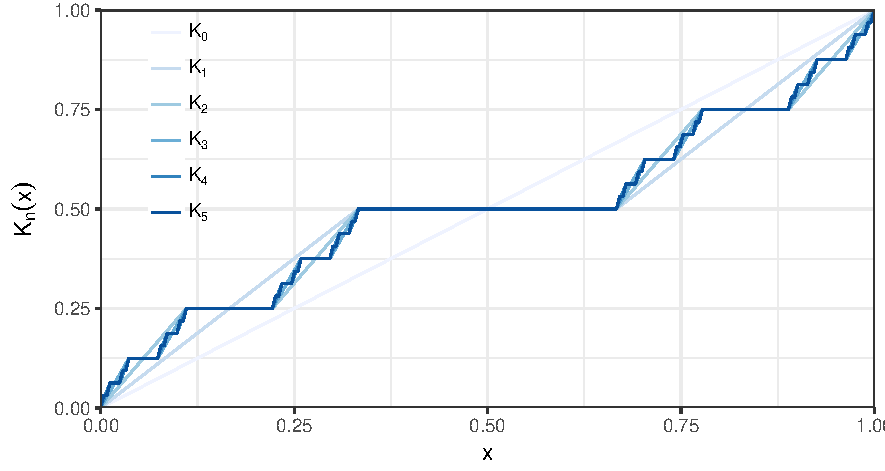
\includegraphics[width=\linewidth]{./img_mas_ejemplos/cantor.pdf}
\caption[Algunos pasos en la \textit{construcción iterativa} de la función de Cantor]{Algunos pasos en la \textit{construcción iterativa} de la función de Cantor, que es creciente, acotada y continua pero no absolutamente continua. En el texto, la función de Cantor es usado para construir medidas con propiedades patológicas.}
\label{img:cantor}
\end{figure}

%La distinción entre variables aleatorias continuas y discretas puede verse más notoria en virtud del teorema \ref{Lebesgue_decomp}.

%\begin{teorema}[Descomposición de Radon-Nikodym]
%Sea $\mu$ una medida definida sobre la $\sigma$-álgebra $\mathcal{B}$, y sea $\nu$ una medida 
%$\sigma$-finita definida sobre $\mathcal{B}$. Entonces $\mu$ puede descomponerse de manera única como
%$\mu = \mu_A + \mu_S$, donde
%\begin{itemize}
%\item $\mu_A$ es absolutamente continua respecto a $\nu$
%\item Existe un conjunto $A$ tal que $\nu(A)=0$, $\mu_S\left(A^{C}\right) = 0$
%\end{itemize}
%\label{Lebesgue_decomp}
%\end{teorema}

%? pagina 109 del manual

%Dado que la medida de Lebesgue es $\sigma$-finita, cualquier medida de probabilidad puede 
%\textit{descomponerse} como la suma de una medida continua, una medida discreta y un \textit{residuo}.

\subsection{Valor esperado}

\begin{definicion}
Sea $X$ una variable aleatoria real y sea $P$ su medida asociada. Se define el \textbf{valor esperado} de $X$ como
\begin{equation}
\E{X} := \int_\Omega X(\lambda) dP(\lambda)
\end{equation}
\end{definicion}

\begin{proposicion}
Sea $X$ una variable aleatoria real, y sea $g$ una función medible en el espacio medible $(\R,\mathcal{B},P_X)$. Entonces $g(X)$ es una variable aleatoria cuyo valor esperado es
\begin{equation}
\E{g(x)} = \int_\Omega [g(X)](\lambda) dP(\lambda) = \int_\R g(x) dP(x)
\end{equation}
\end{proposicion}

\begin{definicion}
Sea $X$ una variable aleatoria real. Si las siguientes cantidades están bien definidas
\begin{align}
\mu_X &{:=} \E{X} \\
\sigma_X^{2} &{:=} \E{(X-\mu_X)^{2}}
\end{align}
entonces se dice que $\mu_X$ es la \textbf{media}\footnote{La notación $\mu_X$ únicamente es usada cuando no hay confusión con la notación para medidas.} de $X$, y $\sigma^2$ es su \textbf{varianza}.
%Por definición, no hay garantía que una variable aleatoria arbitraria tenga media o varianza bien definidas.
\end{definicion}

\begin{ejemplo}
Usando los ejemplos previos sobre variables aleatorias:
\begin{itemize}
\item $X\sim \text{B}(p)$ $\Rightarrow$ $\mu_X = p$ y $\sigma^2_X = p(1-p)$
\item $X\sim D(z)$ $\Rightarrow$ $\mu_X = z$ y $\sigma^2_X = 0$
\item $X\sim \text{N}(\mu,\sigma^{2})$ $\Rightarrow$ $\mu_X = \mu$ y $\sigma^2_X = \sigma^2$
\end{itemize}
\end{ejemplo}

\begin{ejemplo}
Se dice entonces que una variable aleatoria real $X$ sigue una \ul{distribuci\'on de Cauchy} si su función de distribución de probabilidad es de la forma
\begin{equation}
F(x) = \frac{1}{\pi} \mathrm{arc tan}\left( x \right) + \frac{1}{2}
\end{equation}

Es relativamente fácil verificar que la cantidad $\intR x\, dF(x)$ no converge a un número real, y entonces se dice que la media de $X$ no está \textit{bien definida}.
\end{ejemplo}

%De manera más general, se define el $m$-momento de una variable aleatoria $X$ como
%\begin{equation}
%M
%\end{equation}

%\begin{definicion}
%Sea $X$ una varaible aleatoria. Se define su \textbf{función característica} como
%\begin{equation}
%\phi_X (\omega) := \E{e^{i \omega X}} = \int_\R e^{i \omega x} dF_X(x)
%\end{equation}
%donde, para todo $z\in \R$, $e^{i z} := \COS{z} + i \SEN{z}$
%\end{definicion}

\begin{definicion}
Sean $X$, $Y$ dos variables aleatorias, cuyas medidas asociadas son $P_X$ y $P_Y$, y sea $P_{[X,Y]}$ la medida asociada al vector $[X,Y]$. Se define la \textbf{covarianza} entre $X$ y $Y$ como
\begin{equation}
\Cov{X,Y} := \E{X Y} = \int_{\R^{2}} x y\, d P_{[X,Y]}(x,y)
\end{equation}
\end{definicion}

%\begin{proposicion}
%Si $X$, $Y$ son independientes, entonces $\Cov{X,Y} = 0$
%\end{proposicion}
%\begin{proof}
%en la pagina 65 del maual
%\end{proof}

%\begin{definicion}
%Sean $X$, $Y$ dos variables aleatorias. Se define su \textbf{coeficiente de correlación de Pearson} como
%\begin{equation}
%\rho (X,Y) := \sqrt{\frac{\Cov{X,Y}}{\Var{X} \Var{Y}}}
%\end{equation}
%\end{definicion}

\subsection{Vectores aleatorios}

El concepto de variable aleatoria real es sólo un caso particular de variable aleatoria (definición \ref{lazy4}), el cual puede puede usarse para otros conjuntos de interés.
% restringirse a conjuntos más generales \textit{basados} en $\R$, como $\R^{n}$ para algún $n\in \N$.
%
% dicha generalización puede formalizarse fácilmente como otro caso particular.
A continuación se presenta el caso de $\R^{n}$ para algún $n\in \N$.

\begin{definicion}
Se llama \textbf{vector aleatorio} a una variable aleatoria sobre el espacio de probabilidad $(\R^{n},\mathcal{B}^{n},P)$, para algún $n\in \N$. Se define a $\mathcal{B}^{n}$, la $\sigma$-álgebra de Borel $n$-dimensional, como
\begin{equation}
\mathcal{B}^{n} := \sigma\left(\left\{ \left(-\infty, a_1\right]\times \left(-\infty, a_2\right]\times \cdots \times \left(-\infty, a_n\right] \lvert a_1, \dots, a_n \in \R \right\}\right)
\end{equation}
\end{definicion}

Por notación, el vector aleatorio \textit{$n$-dimensional} $\boldsymbol{X}$ será referido como
\begin{equation}
\boldsymbol{X} = [X_1, X_2, \dots, X_n]
\end{equation}
esta notación de vectores con \textit{símbolos gruesos} será usada durante el texto, extendida igualmente para realizaciones y otros vectores similares.

\begin{ejemplo}
Se dice que un vector aleatorio $\boldsymbol{X} = [X_1, X_2, \cdots, X_d]$ sigue una \textbf{distribución multinormal} si su función de probabilidad acumulada conjunta tiene la forma
\begin{equation}
F_{\boldsymbol{X}}\left( \boldsymbol{x} \right) = \frac{1}{\sqrt{(2\pi)^{d}\abso{C}}} \exp\left( -\frac{\boldsymbol{x} C^{-1} \boldsymbol{x}^{\intercal} }{2} \right)
\end{equation}
donde $\boldsymbol{x} = (x_1, x_2, \cdots, x_d)$. El vector $\mu \in \R^{d}$ será referido como \textit{vector de medias}, y la matriz $C \in \R^{d\times d}$ como \textit{matriz de covarianza}.
\end{ejemplo}

% si se necesita, esta en la pagina 30 del manual

%%%%%%%%%%%%%%%%%%%%%%%%%%%%%%%%%%%%%%%%%%%%%%%%%%%%%%%%%%%%%%%%%%%%%%%%%%%%%%%%%%%%%%%%%%%%%%%%%%%

\section{Procesos estocásticos}

Los procesos estocásticos se definen formalmente como variables aleatorias cuyo espacio muestral es un espacio de funciones.
%
Intuitivamente es posible definir %(alternativamente) 
los procesos estocásticos como una \textit{concatenación} de variables aleatorias, es decir, un conjunto de variables aleatorias indexadas sobre algún conjunto arbitrario.
%
Sin embargo, indexar un conjunto infinito de variables aleatorias representa un problema técnico en el cuanto a definir al proceso estocástico como espacio de probabilidad, especialmente al definir la medida de probabilidad asociada.

Debido a las limitaciones del presente trabajo, el tema se expone de manera parcial bajo un enfoque formal; la exposición se basa en aquella presentada por Kolmogorov \cite{kolmogorov2018foundations},
 de modo que el lector interesado debe dirigirse a dicho texto.

Primeramente se define a $\R^{\mathcal{T}}$, el conjunto de funciones con dominio en $\mathcal{T}$ y codominio en $\R$, el cual será usado como espacio de eventos\footnote{Se puede definir análogamente a $\C^{\mathcal{T}}$, o espacios más generales}. 
%
A modo de \textit{intervalos generalizados} se definen los conjuntos de la forma
\begin{equation}
I\left( [t_1, a_1, b_1], \cdots, [t_N, a_N, b_N] \right) = 
\left\{ f \in \R^{\mathcal{T}} \talque f(t_i) \in (a_i, b_i] \, , \, i = 1, \cdots, N \right\}
\end{equation}

Es relativamente fácil extender la familia de estos intervalos por uniones e intersecciones finitas. Es un tanto más interesante definir una $\sigma$-álgebra generada por éstos conjuntos, pero tal parte se omite en el presente trabajo.
%
En el texto por Kolmogorov se explora con mayor detalle la existencia de dicha $\sigma$-álgebra --y por tanto, la existencia de procesos estocásticos.

\begin{definicion}
Un \textbf{proceso estocástico} \xt es una colección de variables aleatorias indexadas por el símbolo $t\in\mathcal{T}$.
\end{definicion}

\begin{definicion}
Se dice que un proceso estocástico \xt es un \textbf{proceso estocástico en $\R$} si cumple que $\mathcal{T} \subseteq \R$.
%
Por notación, el índice $t$ es referido como \textbf{tiempo}, mientras que $\mathcal{T}$ es el conjunto de \textbf{tiempos admisibles}.
\end{definicion}

Por simplicidad, durante el presente trabajo sólo se usarán dos familias de procesos estocásticos en $\R$: si $\mathcal{T}$ es un intervalo, o si es parte de una \textit{malla}. 
%
La primera familia se reserva para modelar las señales electrofisiológicas, mientras que la segunda se usará para modelar los registros de estas mismas señales.
%
La distinción consiste en que las señales electrofisiológicas sólo pueden ser registradas digitalmente en un conjunto finito de puntos en el tiempo; la atención del texto recae en ambos grupos de procesos, en espera que sus características sean similares de algún modo.

\begin{definicion}
Se dice que un proceso estocástico en $\R$ es \textbf{a tiempo continuo} si existen $a, b \in \R \cup \{ -\infty, \infty \}$ tales que
\begin{equation}
\mathcal{T} = (a,b)
\end{equation}
Así mismo, se dice que un proceso estocástico en $\R$ es \textbf{a tiempo discreto} si existen $t_0, \Delta_X \in \R \cup \{ -\infty, \infty \}$ tales que
\begin{equation}
\mathcal{T} = \left\{ t_0 + t \in \R \talque {t} \cdot {\Delta_X} \in \Z \right\}
\end{equation}
Por notación, $\Delta_X$ es referida como \textit{frecuencia de muestreo}.
\end{definicion}

Conviene destacar que el nombre \textit{frecuencia de muestreo} hace referencia al proceso de registro, que algunos textos es referido como \textit{muestreo}; esta terminología entra claramente en conflicto con las muestras de una variable aleatoria. En lo siguiente se evita llamar muestreo al proceso de registro, pero se conservará el término frecuencia de muestro.

Cabe mencionar que hay un conflicto similar con los términos \textit{tiempo continuo} y \textit{tiempo discreto}; estos términos \underline{no guardan ninguna analogía} con las variables aleatorias discretas y continuas, ni con los espectro de potencias puramente continuos o puramente discretos (ver el capítulo siguiente).
%
Estos términos se usan porque se encuentran muy extendidos en la literatura sobre análisis de señales.

Para facilitar la referencia de procesos estocásticos, los elementos que lo componen son denotados como:
\begin{description}
\item[\xt]        Todo el proceso.
\item[$X(t)$]     Variable aleatoria en el proceso, para el tiempo $t \in \mathcal{T}$.
\item[$x(t)$]     Una observación de $X(t)$, para el tiempo $t \in \mathcal{T}$.
\item[$F_{X(t)}$] Función de probabilidad acumulada para $X(t)$.
\end{description}
%\begin{tabular}{cl}
%\xt    & Todo el proceso \\
%$X(t)$ & Variable aleatoria en el proceso, para el tiempo $t$ \\
%$x(t)$ & Una realización de $X(t)$ \\
%$F_{X(t)}$ & Función de probabilidad acumulada para $X(t)$
%%$ {\Delta_t}$ & Frecuencia de muestreo (en tiempo discreto)
%\end{tabular}

\subsection{Estacionariedad débil}

De forma general, la estacionariedad significa que \textit{algunas} propiedades de un proceso sean \textit{invariantes} en el tiempo; la decisión sobre qué características deben ser invariantes, y en qué sentido, conlleva a diferentes definiciones.
%
Por ejemplo, en la definición \ref{est_fuerte} se pide que todas las variables que integra al proceso sigan una distribución común, así como todas variables conjuntas con algunas características.

\begin{definicion}%[Estacionariedad fuerte]
Un proceso \xt se dice \textbf{fuertemente estacionario} si para cualesquiera $t_1, t_2, \dots, t_n \in \mathcal{T}$ y cualquier $\tau$ tal que $t_i + \tau \in \mathcal{T}$, se cumple que
\begin{equation*}
F_{\left[ X(t_1), X(t_2), \dots, X(t_n) \right]} \equiv
F_{\left[ X(t_1 + \tau), X(t_2 + \tau), \dots, X(t_n + \tau) \right]}
\end{equation*}
con $F_{[v_1,v_2,\dots,v_N]}$ es la función de probabilidad acumulada para el vector $[v_1,v_2,\dots,v_N]$.
\label{est_fuerte}
\end{definicion}

En el contexto del presente trabajo la estacionariedad fuerte se considera \textit{innecesariamente fuerte}, en cuanto a que es difícil de verificar y porque se usarán hipótesis más débiles.
%
Se decidió conveniente una definición que garantice que los momentos puedan ser estimados, para lo cual deben ser constantes en el tiempo.
%
La motivación principal para ello es el siguiente: si se modela una señal como proceso estocástico, entonces los momentos están asociados con variables físicas relevantes. 
%
En particular, el segundo momento está asociado con la \textit{energía} (definición \ref{lazy5}).

\begin{definicion}%[Estacionariedad de orden $m$]
Un proceso \xt se dice \textbf{estacionario de orden $\boldsymbol{m}$} si, para cualesquiera $t_1, t_2, \dots, t_n \in \mathcal{T}$ y cualquier $\tau$ tal que $t_i + \tau \in \mathcal{T}$, se cumple que
\begin{equation*}
\E{X^{m_1}(t_1)X^{m_2}(t_2)\cdots X^{m_n}(t_n)} =
\E{X^{m_1}(t_1+\tau)X^{m_2}(t_2+\tau)\cdots X^{m_n}(t_n+\tau)}
\end{equation*}
para cualesquiera enteros $m_1, m_2, \dots, m_n$ tales que $m_1+m_2+\cdots+m_n \leq m$.
\label{est_m}
\end{definicion}

La definición \ref{est_m} es conveniente tomando en cuenta que para estudiar la energía de un proceso (asociada al segundo momento) requerirá poner condiciones adicionales; por ejemplo, para estimar la varianza de la energía en un proceso, a partir de observaciones, se requiere que el proceso sea estacionario de orden 4.
%
En el otro sentido, siempre que sea posible se usará la menor cantidad de hipótesis, para lo cual se presenta una definición más particular y \textit{débil} de estacionariedad.

\begin{definicion}%[Estacionariedad débil]
Un proceso \xt se dice \textbf{débilmente estacionario} si existen constantes $\mu, \sigma \in \R$ y una función $R : \mathcal{T} \rightarrow \R \cup \{ \pm \infty \} $ tales que, para cualesquiera $t, s \in T$ se 
cumple
\begin{itemize}
\item $\E{X(t)} = \mu$
\item $\Var{X(t)} = \sigma^{2}$
\item $\Cov{X(t),X(s)} = R(\abso{s-t})$
\end{itemize}
\end{definicion}

\begin{proposicion}
Para que un proceso estocástico \xt sea débilmente estacionario es suficiente y necesario que sea estacionario de orden 2.
\end{proposicion}

%\begin{proof}
%\ul{Para probar que la condición es necesaria} supóngase que \xt es débilmente estacionario.
%Para que sea estacionario de orden 2 debe cumplirse que, para cualesquiera $s, t, s+\tau, y+\tau \in \mathcal{T}$
%\begin{enumerate}
%\item $\E{X(t)} = \E{X(t+\tau)}$
%\item $\E{X^{2}(t)} = \E{X^{2}(t+\tau)}$
%\item $\E{X(t)X(s)} = \E{X(t+\tau)X(s+\tau)}$
%\end{enumerate}
%
%\ul{Para probar que la condición es necesaria} supóngase que \xt es estacionario de orden 2.
%%
%Se toma un $t_0\in \mathcal{T}$ arbitrario, y se define
%\begin{equation*}
%\mu = \E{X(t_0)} \qquad \sigma^{2} = \Var{X(t_0)}
%\end{equation*}
%\end{proof}

El que un proceso sea débilmente estacionario implica la existencia de una media y varianza características del proceso, es decir, que son comunes a todas las variables aleatorias que lo componen. 
%
Además, se implica la existencia de una función referida como \textit{autocovarianza}.

\begin{definicion}
Sea \xt un proceso estocástico sobre $\R$. Su \textbf{función de autocovarianza} es una función $R: \R^{2}\rightarrow \R$ tal que
\begin{equation}
R(t,s) = \E{\left(X(t) - \E{X(t)}\right)\overline{\left(X(s) - \E{X(s)}\right)}}
\end{equation} 
para cualesquiera tiempos admisibles $s, t \in \mathcal{T}$.
\end{definicion}

Como las señales electrofisiológicas son modeladas como procesos estocásticos, conviene traducir algunas de sus características en propiedades para los procesos estocásticos.
%
Por ejemplo, se sabe que las señales representan variaciones en campos eléctricos, y entonces se puede afirmar sin duda que dicha cantidad es finita en todo momento; lo mismo se puede afirmar sobre la energía.
%
En base a ello, los procesos estocásticos que modelan señales electrofisiológicas deben tener energía y varianza finitas en todo momento.
%
Más aún, la actividad eléctrica cerebral y muscular presentan durante el reposo una actividad característica, referida como \textit{actividad basal} o \textit{línea base}, que es relativamente cercana a una constante en todo momento (ver figura \ref{ejemplos_mor}).
%
El fenómeno de línea base entra en el modelado como el supuesto de que las señales son procesos estacionarias de orden 1; por simplicidad, se puede considerar que la media de estos procesos es 0.

Una segunda característica de las señales que se traduce es la continuidad: las señales representan fenómenos eléctricos que cambian de manera \textit{suave} en el tiempo.
%
El aspecto de los registros con \textit{picos} se explica porque el cambio es suave, pero es muy rápido respecto a la tasa de registro.

\begin{proposicion}
Sea \xt un proceso débilmente estacionario y $R$ su función de autocovarianza. Si $R$ es continua
en 0 entonces es continua en todo $\R$.
\end{proposicion}

\begin{proof}
Supóngase que $R$ es continua en 0. Tómese a $t_0 \in \mathcal{T}$ arbitrario para verificar que $R$ es continua en $t_0$, y tómense $s,h$ tales que $s,s+t,s+t+h \in\mathcal{T}$. Usando la desigualdad de Schwarz, puede escribirse que
\begin{align*}
\left[ R(t_0+h) -R(t_0) \right]^{2} 
&= \left( \E{X(s+t_0+h)X(s)} - \E{X(s+t_0)X(s)} \right)^{2}  \\
&= \left( \E{X(s)\left[ X(s+t_0+h) - X(s+t_0) \right]} \right)^{2} \\
&\leq \E{\left( X(s) \right)^{2}} \E{\left( X(s+t_0+h) - X(s+t_0) \right)^{2}} \\
&\leq 2 \sigma_X^{2} \left[ \sigma_X^{2} - R(h) \right]
\end{align*}
Entonces, puede afirmarse que
\begin{equation*}
\abso{R(t_0+h) -R(t_0)} \leq \sqrt{2 \sigma_X^{2}} \sqrt{R(0) - R(h)}
\end{equation*}
Como $R$ es continua en 0, entonces 
\begin{align*}
\lim_{h\rightarrow 0} (R(0)-R(h)) = 0 &\Rightarrow \lim_{h\rightarrow 0} (R(t_0+h)-R(t_0)) = 0
\end{align*}
de donde se concluye que $R$ es continua en $t_0$, para cualquier $t_0\in \mathcal{T}$.
\end{proof}    

\begin{definicion}%[Continuidad estocástica en media cuadrática]
Un proceso a tiempo continuo \xt se dice \textbf{estocásticamente continuo, en el sentido de media cuadrática}, en el tiempo $t_0\in \mathcal{T}$ si
\begin{equation*}
\lim_{t \rightarrow t_0} \E{\left( X(t) - X(t_0) \right)^{2}} = 0
\end{equation*}
\label{cont_est}
\end{definicion}

Por simplicidad, y porque es la única definición de su tipo usada en el presente trabajo, la continuidad estocástica en media cuadrática será referida simplemente como \textit{continuidad estocástica}.

\begin{proposicion}
Sea \xt un proceso a tiempo continuo, débilmente estacionario y de media cero, y sea $R$ su función de autocovarianza. El proceso es estocásticamente continuo en $t_0\in \mathcal{T}$ si y sólo si $R$ es continua en $0$.
\label{lazy:aaa}
\end{proposicion}

\begin{proof}
Para cualquier $t\in \mathcal{T}$, puede escribirse
\begin{align*}
\E{\left( X(t) - X(t_0) \right)^{2}} &= \Var{X(t)} + \Var{X(t_0)} - 2 \Cov{X(t),X(t_0)} \\
&= 2 \left( \sigma_X^{2} - R(t-t_0) \right) \\
&= 2 \left( R(0) - R(t-t_0) \right)
\end{align*}
Así entonces, la condición para continuidad estocástica puede reescribirse como
\begin{align*}
\lim_{t \rightarrow t_0} \E{\left( X(t) - X(t_0) \right)^{2}} = 0 
&\Leftrightarrow
\lim_{t \rightarrow t_0} \left( R(0) - R(t-t_0) \right) = 0 \\
&\Leftrightarrow
\lim_{\tau \rightarrow 0} R(\tau) = R(0)
\end{align*}
\end{proof}

\begin{definicion}
Se dice que una función $f: \R\rightarrow \R$ es \textbf{definida positiva} si para cualesquiera $x_1, _2, \cdots, x_N \in \R$, $z_1, z_2, \cdots, z_N \in \R$ se cumple que 
\begin{equation}
\sum_{n=1}^{N} \sum_{m=1}^{N} z_n z_m f(x_m-x_n) \leq 0
\end{equation}
\end{definicion}

\begin{proposicion}
Sea \xt un proceso débilmente estacionario y $R$ su función de autocorrelación. Se cumple que $R$ es una función positiva definida.
\label{lazy:meh}
\end{proposicion}

\begin{proof}
Sean $t_1, t_2, \cdots, t_N \in \mathcal{T}$, $z_1, z_2, \cdots, z_N \in \R$ arbitrarios. Se construye la variable aleatoria $W$ como
\begin{equation}
W = \sum_{n=1}^{N} z_n X(t_n)
\end{equation}

Ahora, nótese que
\begin{align*}
0 &\leq \Var{W} \\
&= \sum_{m=1}^{N} \sum_{n=1}^{N} z_m z_n \Cov{X(t_m),X(t_n)} \\
&= \sum_{m=1}^{N} \sum_{n=1}^{N} z_m z_n R(t_m-t_n)
\end{align*}
\end{proof}

\begin{ejemplo}
Un \underline{proceso oscilante} es un proceso estocástico $\{ S(t)\}_{t\in\R}$ definido como
\begin{equation}
S(t) = \COS{t + \phi}
\end{equation}
donde $\phi \sim \text{unif}(-\pi,\pi)$.
%, es decir
%
Es muy notable que el proceso esté \textit{caracterizado} por una única variable aleatoria y que sus realizaciones siempre son funciones \textit{suaves}, contrario al estereotipo para estas funciones.

Su valor esperado puede ser calculado fácilmente
\begin{align}
\E{S(t)} &= \E{\COS{t + \phi}} = \frac{1}{2 \pi} \int_{-\pi}^\pi \COS{t + \phi} d\phi = 0
\end{align}

Similarmente para la función de autocovarianza
\begin{align*}
\E{S(t)S(s)} &= 
\E{\COS{t + \phi}\COS{s + \phi}} \\
&=
\E{\frac{1}{2} \COS{t-s} + \frac{1}{2}\COS{t+s+2\phi}} \\
&=
\frac{1}{2} \COS{t-s} + \frac{1}{2} \E{\COS{t+s+2\phi}} \\
&= \frac{1}{2} \COS{t-s}
\end{align*}

Se concluye que $\{ S(t)\}_{t\in\R}$ es débilmente estacionario.
%
Un segundo aspecto notorio en este ejemplo es que la función de autocovarianza es periódica, contrario al estereotipo de que las funciones autocorrelación siempre decaen exponencialmente.
\end{ejemplo}

\begin{ejemplo}
Un \underline{proceso ruido blanco} es un proceso estocástico $\{ \varepsilon(t)\}_{t\in\R}$ tal que si $t, s\in \R$ son diferentes entonces $\varepsilon(t)$ y $\varepsilon(s)$ son indepentiendes.
%
Se dice que el proceso ruido blanco es `normal' si $\varepsilon(t) \sim N(0,1)$.
%$\varepsilon(t) \sim N(0,\sigma^2)$ para algún $\sigma\in\R$. 
%
Por simplicidad, el término ruido blanco será usado de forma general para procesos normales estándar, con el fin de garantizar que son débilmente estacionarios.

La función de autocovarianza de un proceso ruido blanco es
\begin{equation}
R(\tau) = \begin{cases}
\sigma^2 &, \tau = 0 \\
0 &, \text{otro caso}
\end{cases}
\end{equation}
Se concluye que el proceso ruido blanco es débilmente estacionario, pero no es estocásticamente continuo.
\end{ejemplo}

Antes de pasar a otro tema conviene mencionar enfáticamente que la covarianza es una medida de asociación lineal entre variables aleatorias, pero \textbf{no} puede usarse como medida de independencia.
%
Como se muestra en el siguiente ejemplo, es perfectamente posible generar variables cuya covarianza es cero pero que no son independientes.

\begin{ejemplo}
Sea $\{ \varepsilon(n)\}_{n\in\Z}$ un proceso ruido blanco normal estándar, a tiempo discreto. Se construye al proceso $\{ \nu(n)\}_{n\in\N}$ como
\begin{equation}
\nu(n) = \varepsilon(n)\varepsilon(n-1)
\end{equation}

Es relativamente fácil notar que el proceso es de media 0
%
La función de autocovarianza del proceso, $R$, admite tres casos relevantes
\begin{itemize}
\item Si $\tau=0$, para cualquier $n\in \Z$
\begin{equation}
\E{\nu(n)^2} = \E{\varepsilon(n)^2\varepsilon(n-1)^2} = \E{\varepsilon(n)^2}\E{\varepsilon(n-1)^2} = 
1
\end{equation}
\item Si $\abso{\tau}=1$, para cualquier $n\in \Z$
\begin{equation}
\E{\nu(n)\nu(n+1)} = \E{\varepsilon(n)^2\varepsilon(n-1)\varepsilon(n+1)} = \E{\varepsilon(n)^2}\E{\varepsilon(n-1)}\E{\varepsilon(n+1)} = 0
\end{equation}
\item Si $\abso{\tau}>1$, para cualquier $n\in \Z$
\begin{equation}
\E{\nu(n)\nu(n+\tau)} = \E{\nu(n)}\E{\nu(n+\tau)} = 0
\end{equation}
\end{itemize}

%%
Claramente $\{ \nu(n)\}_{n\in\N}$ no es un proceso ruido blanco, ya que se compone de variables aleatorias que no son independientes.
%
Sin embargo, su función de autocovarianza es la misma que para un proceso ruido blanco, mostrando que se compone de variables que no están asociadas linealmente. 
\end{ejemplo}

\begin{figure}
\centering
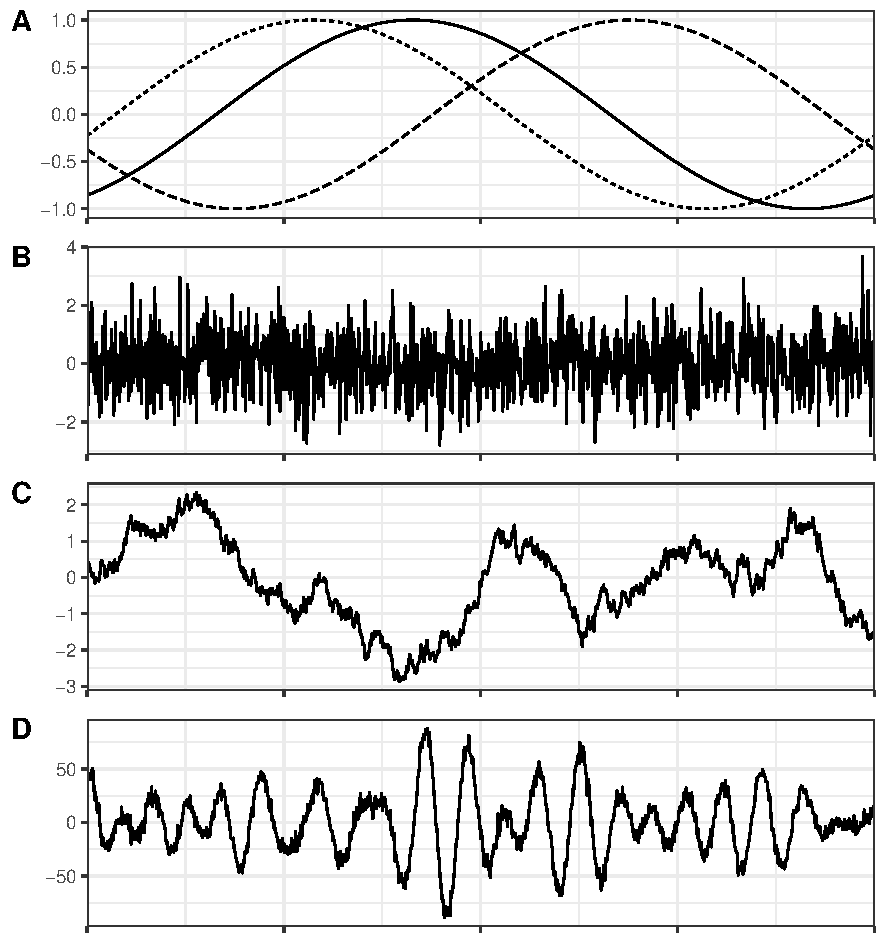
\includegraphics[width=\linewidth]{./img_mas_ejemplos/ruidos_ejemplos.pdf}
\caption[Ejemplos de procesos estocásticos.]{Ejemplos de realizaciones para algunos procesos estocásticos. \textbf{A.} Proceso oscilante, del cual se grafican tres realizaciones diferentes. \textbf{B.} Proceso Ruido Blanco. \textbf{C.} Proceso de Wiener. \textbf{D.} Proceso medias móviles a tiempo continuo con parámetro $A=\nicefrac{1}{4}$. 
%\textbf{D.} Proceso tipo alfa. 
}
\end{figure}

\subsection{Integración y procesos estocásticos}
\label{sec:int_proc_est}

La integral, según las definiciones \ref{def:lazy1} y \ref{def:lazy2}, puede extenderse intuitivamente respecto a un proceso estocástico.
%
Este tema no será explorado con mayor detalle en el presente texto, sino que sólo será usado para construir algunos ejemplos.
%
Para ello se define al proceso de Wiener, un proceso estocástico con algunas propiedades peculiares que serán de gran utilidad.

\begin{ejemplo}
Un \underline{proceso de Wiener} es un proceso estocástico $\{ W(t)\}_{t\in\R}$ que satisface las siguientes propiedades para cualesquiera $t, s, \in \R$
\begin{itemize}
\item $W(0) \sim \text{D}(0)$
\item $\left[W(t)-W(s)\right] \sim N(0, \abso{t-s})$
\item $\left[W(t)-W(s)\right]$ es independiente de $W(u)$ para $u < \min\{ t, s \}$
\end{itemize}

Es relativamente fácil notar que $\E{W(t)} = 0$ y $\E{\left(W(t)\right)^2}$, de donde se deduce que el proceso de Wiener no es débilmente estacionario.
\end{ejemplo}

Así entonces, sea $\{ W(t)\}_{t\in\R}$ un proceso de Wiener, $[a,b]\subseteq\R$ un intervalo arbitrario, y $f:[a,b]\longrightarrow\R_+$ una función medible.
%
Sean $t_1, t_2, \dots, t_N \in \R$ una partición arbitraria de $[a,b]$, es decir que satisfacen
\begin{equation}
a < t_1 < t_2 < \dots < t_N < b
\end{equation}
entonces se define la variable aleatoria
\begin{equation}
\sum_{i=2}^N \left[ \sup_{\lambda \in [t_{i-1},t_i]} f(\lambda) \right] \left[ W(t_i) - W(t_{i-1}] \right)
\end{equation}

\underline{Si} la colección de variables aleatorias converge en media cuadrática entonces se dice que
\begin{equation}
\int_a^b f(t) dW(t) :=
\lim_{N\rightarrow \infty} \left(
\sum_{i=2}^N \left[ \sup_{\lambda \in [t_{i-1},t_i]} f(\lambda) \right] \left[ W(t_i) - W(t_{i-1}] \right] \right)
\end{equation}

\begin{proposicion}
Sea $\{ W(t)\}_{t\in\R}$ un proceso de Wiener, $[a,b]\subseteq\R$ un intervalo arbitrario, y $f:[a,b]\longrightarrow\R_+$ una función medible. Entonces
\begin{equation}
\E{\int_a^b f(t) dW(t) } = 0
\end{equation}
\label{prop:lazy000}
\end{proposicion}
\begin{proof}
Sea $\Delta W_i = W(t_i) - W(t_{i-1})$, el cual satisface las siguientes propiedades
\begin{itemize}
\item $\E{\Delta W_i} = 0$
\item $\E{\left( \Delta W_i \right)^2} = t_{i} - t_{i-1}$
\item Si $i<j$ entonces $\Delta W_i$ y $\Delta W_j$ son independientes
\end{itemize} 

Entonces, nótese que
\begin{align*}
\E{\int_a^b f(t) dW(t) } &=
\E{ \lim_{N\rightarrow \infty} \left( \sum_{i=2}^N f_i \Delta W_i \right) } \\
&= 
\lim_{N\rightarrow \infty} \left( \sum_{i=2}^N f_i \E{ \Delta W_i } \right) \\
&= 0
\end{align*}
donde $f_i = \sup_{\lambda \in [t_{i-1},t_i]} f(\lambda)$.
\end{proof}

\begin{proposicion}
Sea $\{ W(t)\}_{t\in\R}$ un proceso de Wiener, $[a,b]\subseteq\R$ un intervalo arbitrario, y $f:[a,b]\longrightarrow\R_+$ una función medible. Entonces
\begin{equation}
\E{\left(\int_a^b f(t) dW(t) \right)^2 } = \int_a^b \left[ f(t) \right]^2 dt
\end{equation}
\label{prop:lazy100}
\end{proposicion}
\begin{proof}
Sea $\Delta W_i = W(t_i) - W(t_{i-1})$, como en la demostración anterior.
Nótese que
\begin{align*}
\E{\left(\int_a^b f(t) dW(t) \right)^2 } &=
\E{\left( \lim_{N\rightarrow \infty} \left(
\sum_{i=2}^N f_i \Delta W_i \right) \right)^2} \\
&= 
\lim_{N\rightarrow \infty} \E{ \left(
\sum_{i=2}^N f_i \Delta W_i \right)^2} \\
&=
\lim_{N\rightarrow \infty} \sum_{i=2}^N \sum_{j=2}^N
f_i f_j \E{  \Delta W_i \Delta W_j } \\
&=
\lim_{N\rightarrow \infty} \sum_{i=2}^N
f_i^2 \E{  \left( \Delta W_i \right)^2 } \\
&=
\lim_{N\rightarrow \infty} \sum_{i=2}^N
f_i^2 (t_i-t_{i-1}) \\
&=
\int_a^b \left[ f(t) \right]^2 dt
\end{align*}
donde $f_i = \sup_{\lambda \in [t_{i-1},t_i]} f(\lambda)$.
\end{proof}

\begin{ejemplo}
Sea $\{ W(t)\}_{t\in\R}$ un proceso de Wiener y sea $A\in\R_+$ arbitrario. Se define a $\{Y(t)\}_{t\in\R}$, un \underline{proceso medias m\'oviles tiempo continuo} con parámetro $A$, como
\begin{equation}
Y(t) = \frac{1}{A}\int_{t-\nicefrac{A}{2}}^{t+\nicefrac{A}{2}} dW(u)
\end{equation}

Con base a la proposición \ref{prop:lazy000}, se deduce que
\begin{equation}
\E{Y(t)} = 0
\end{equation}
Así mismo, usando la proposición \ref{prop:lazy100} se deduce la función de autocovarianza
%\begin{align*}
%\E{Y(t)Y(s)} &= 
%\E{ \left( \frac{1}{A}\int_{\Omega_t} dW(u) \right) \left( \frac{1}{A}\int_{\Omega_s} dW(v)\right) } \\
%&= 
%\frac{1}{A^2} 
%\E{ 
%\left( 
%\int_{\Omega_t \cap \Omega_s^C} dW(u) + \int_{\Omega_t \cap \Omega_s} dW(u) 
%\right)
%\left( 
%\int_{\Omega_s \cap \Omega_t^C} dW(v) + \int_{\Omega_t \cap \Omega_s} dW(v) 
%\right)  
%} \\
%&=
%\frac{1}{A^2} 
%\E{ 
%\left( 
%\int_{\Omega_t \cap \Omega_s^C} dW(u)  
%\right)
%\left( 
%\int_{\Omega_s \cap \Omega_t^C} dW(v) 
%\right)  
%} \\
%&\pheq
%+ \frac{1}{A^2} 
%\E{ 
%\left( 
%\int_{\Omega_t \cap \Omega_s^C} dW(u)  
%\right)
%\left( 
% \int_{\Omega_t \cap \Omega_s} dW(v) 
%\right)  
%} \\
%&\pheq
%+\frac{1}{A^2} 
%\E{ 
%\left( 
%\int_{\Omega_t \cap \Omega_s} dW(u) 
%\right)
%\left( 
%\int_{\Omega_s \cap \Omega_t^C} dW(v)
%\right)  
%} \\
%&\pheq
%+\frac{1}{A^2} 
%\E{ 
%\left( 
%\int_{\Omega_t \cap \Omega_s} dW(u) 
%\right)
%\left( 
%\int_{\Omega_s \cap \Omega_t^C} dW(v)
%\right)  
%} \\
%&=
%\frac{1}{A^2} 
%\E{  
%\int_{\Omega_t \cap \Omega_s^C} dW(u)  
%}
%\E{
%\int_{\Omega_s \cap \Omega_t^C} dW(v) 
%} \\
%&\pheq
%+ \frac{1}{A^2} 
%\E{ 
%\int_{\Omega_t \cap \Omega_s^C} dW(u)  
%}
%\E{
% \int_{\Omega_t \cap \Omega_s} dW(v) 
%} \\
%&\pheq
%+\frac{1}{A^2} 
%\E{ 
%\int_{\Omega_t \cap \Omega_s} dW(u) 
%}
%\E{
%\int_{\Omega_s \cap \Omega_t^C} dW(v)
%} \\
%&\pheq
%+\frac{1}{A^2} 
%\E{ 
%\left( 
%\int_{\Omega_t \cap \Omega_s} dW(u) 
%\right)^2
%} \\
%&= \frac{1}{A^2} \max \{ 1-\abso{t-s}, 0 \}
%\end{align*}
\begin{align*}
\E{Y(t)Y(s)} &= 
\E{ \left( \frac{1}{A}\int_{\Omega_t} dW(u) \right) \left( \frac{1}{A}\int_{\Omega_s} dW(v)\right) } \\
&= 
\frac{1}{A^2} 
\E{ 
\left( 
\int_{\Omega_t \cap \Omega_s^C} dW(u) + \int_{\Omega_t \cap \Omega_s} dW(u) 
\right)
\left( 
\int_{\Omega_s \cap \Omega_t^C} dW(v) + \int_{\Omega_t \cap \Omega_s} dW(v) 
\right)  
} \\
&=
\frac{1}{A^2} 
\E{  
\int_{\Omega_t \cap \Omega_s^C} dW(u)  
}
\E{
\int_{\Omega_s \cap \Omega_t^C} dW(v) 
} \\
&\pheq
+ \frac{1}{A^2} 
\E{ 
\int_{\Omega_t \cap \Omega_s^C} dW(u)  
}
\E{
 \int_{\Omega_t \cap \Omega_s} dW(v) 
} \\
&\pheq
+\frac{1}{A^2} 
\E{ 
\int_{\Omega_t \cap \Omega_s} dW(u) 
}
\E{
\int_{\Omega_s \cap \Omega_t^C} dW(v)
} \\
&\pheq
+\frac{1}{A^2} 
\E{ 
\left( 
\int_{\Omega_t \cap \Omega_s} dW(u) 
\right)^2
} \\
&= \frac{1}{A^2} \max \{ A-\abso{t-s}, 0 \}
\end{align*}
donde $\Omega_t = \left[ t - \nicefrac{A}{2}, t + \nicefrac{A}{2} \right]$ y similarmente para $\Omega_s$.
%
En particular, el proceso de medias móviles a tiempo continuo es débilmente estacionario.
%
Por simplicidad, este proceso será referido simplemente como \textit{proceso medias móviles}.
\end{ejemplo}

%%%%%%%%%%%%%%%%%%%%%%%%%%%%%%%%%%%%%%%%%%%%%%%%%%%%%%%%%%%%%%%%%%%%%%%%%%%%%%%%%%%%%%%%%%%%%%%%%%%

\section{Estimación de parámetros}

Hasta ahora se ha hablado de las variables aleatorias y procesos estocásticos únicamente como objetos definidos formalmente.
%
En el contexto del presente trabajo, dichos objetos son usados para modelar fenómenos físicos, es decir que se espera que ciertos fenómenos presenten comportamientos similares a cierto tipo de variables aleatorias.
%
%La selección de los modelos en sí no será discutida en este capítulo.
%
En esta sección se aborda el problema formal de \textit{recuperar} información sobre estos objetos en base a las observaciones obtenidas del fenómeno estudiado, las cuales son interpretadas como \textit{huellas} de estos objetos aleatorios.

%Es común que se conozca cierta información de estos fenómenos que permita suponer que se comportan como variables aleatorias con cierta forma. Por ejemplo, ?.%se suele suponer que entre la población, 
%%
%Conviene destacar el caso de fenómenos que son \textit{forzados} a seguir una distribución conocida; por ejemplo, la metodología para aplicar la prueba Neuropsi \cite{Ostrosky00} ha sido diseñada de tal forma que los puntajes siguen una distribución normal para cada segmento poblacional.

%\begin{definicion}
Considérese a $X$, una variable aleatoria entre los espacios medibles $(\Omega_1,\mathcal{U}_1)$ y $(\Omega_2,\mathcal{U}_2)$. 
%
Para poder \textit{conectar} a $X$ con el fenómeno estudiado, $\Omega_1$ debe incluir todas los estados posibles del sistema bajo las condiciones de estudio; mientras, $\Omega_2$ es típicamente un conjunto \textit{basado} en $\R$ suficientemente general para cuantificar \textit{adecuadamente} a las mediciones hechas sobre el sistema.
%
Con un conjunto basado en $\R$ se engloba informalmente al mismo $\R$, alguno de sus subconjuntos, a $\C$, a $\R^n$ para algún $n\in \N$, o incluso a $\R^\mathcal{T}$, entre otros.
%\end{definicion}

En concreto, se considera el problema en que la variable aleatoria modelo, $X$, admite una función de probabilidad acumulada $F(\bullet; \theta)$ que depende de un parámetro $\theta \in \Theta$, donde $\Theta$ es referido como \textbf{espacio de parámetros}.
%
El objetivo es deducir el valor de $\theta$ a partir de las observaciones recabadas.

\begin{definicion}
Sea $X$ una variable aleatoria real. Una \textbf{muestra de $\boldsymbol{X}$ de tamaño $\boldsymbol{N}$} es una colección de variables aleatorias $\{ X_1, X_2, \dots, X_N \}$ tales que son independientes y comparten la misma distribución que $X$.
%
Mientras no se indique lo contrario, las variables aleatorias en la muestra no están ordenadas.
\end{definicion}

\begin{proposicion}
Sea $X$ una variable aleatoria continua, sea $f_X$ su función de densidad de probabilidad, y sea $\{ X_1, \dots, X_N \}$ una muestra de tamaño $N$. 
%
La función de densidad de probabilidad conjunta para el vector $\boldsymbol{X}=[ X_1, X_2, \dots, X_N ]$ es
\begin{equation}
f_{\boldsymbol{X}}(x_1, \dots, x_N ) = \prod_{j=1}^{N} f(x_j)
\end{equation}
\label{oculto1}
\end{proposicion}

\begin{definicion}
Sea $X$ una variable aleatoria y sea $\{ X_1, \dots, X_N \}$ una muestra de tamaño $N$.
%
Un \textbf{estadístico} es una función $\widehat{\theta}: \R^{n}\rightarrow\R$ evaluada en la muestra.

Si se pretende que el valor del estadístico sea \textit{parecido} a un parámetro $\theta$, entonces se dice que el estadístico $\widehat{\theta}$ es un \textbf{estimador} de $\theta$.
\end{definicion}

%\begin{proposicion}
%Sea $X$ una variable aleatoria, $\{ X_1, X_2, \dots, X_N \}$ una muestra y $\{ x_1, x_2, \dots, x_N \}$ un conjunto de observaciones. Se define la \textbf{función de distribución muestral} como
%\begin{equation}
%F_{X; N} (x) := \frac{1}{N} \sum_{x_j \leq x } 1
%\end{equation}
%\end{proposicion}

%\begin{proposicion}
%Si el tamaño de una muestra de $X$ se vuelve arbitrariamente grande, la función de distribución muestral converge en probabilidad a $F$, la función de probabilidad acumulada de $X$
%\begin{equation}
%\lim_{N \rightarrow \infty} F_{X; N} = F_X
%\end{equation}
%\end{proposicion}

%\begin{proof}
%Ver seccion 5.2 C R Rao, Linear Statistic Inference and its applications 2 ed pag 42
%\end{proof}

%\begin{teorema}[Cramér-Rao]
%Sea $\widehat{\theta}$ un estimador insesgado de $\theta$. Si la función de verosimilitud asociada al estimador, $L$, es diferenciable, entonces
%\begin{equation}
%\Var{\widehat{\theta}} \geq \left( \E{\frac{\partial}{\partial\theta} L(X; \theta)} \right)^{-2}
%\end{equation}
%La igualdad se alcanza si y sólo si existe una función positiva $k$ tal que puede escribirse
%\begin{equation}
%\frac{\partial}{\partial\theta} L(X; \theta) = k(\theta) \left[ \widehat{\theta}(X) - \theta \right] 
%\end{equation}
%\end{teorema}

%\begin{definicion}
%Sea $X$ una variable aleatoria que depende de un parámetro $\theta$ y $X_1, \dots, X_N$ una muestra de tamaño $N$. Un estimador $\widehat{\theta}$ es \textbf{suficiente} si
%la distribución de la variable $X \lvert \widehat{\theta}$ no depende de $\theta$
%\end{definicion}

%\begin{teorema}
%Sea $X$ una variable aleatoria que depende del parámetro $\theta$. Un estadístico $\widehat{\theta}$ es suficiente si y sólo si existen funciones $g$ y $h$ tales que
%\begin{equation}
%f_X(\bullet; \theta ) = g(\widehat{\theta},\theta) h_X(\bullet)
%\end{equation}
%\end{teorema}
%\begin{proof}
%ver pagina 121 del libro de lindgren
%\end{proof}

%Usando la desigualdad de Chebyshev de puede deducir que
%\begin{equation}
%P\left( \abso{\widehat{\theta} - \theta} > \varepsilon \right) \leq 
%\frac{1}{\varepsilon^{2}} \E{\left( \widehat{\theta} - \theta \right)^{2}}
%\end{equation}

%\begin{definicion}
%El \textbf{error de media cuadrática} para el estimador $\widehat{\theta}$ se define como
%\begin{equation}
%\text{EMC}(\widehat{\theta}) := \E{\left( \widehat{\theta} - \theta \right)^{2}} =
%\Var{\widehat{\theta}} + \left( \E{\theta} - \theta^{2} \right)
%\end{equation}
%\end{definicion}

\begin{definicion}
Sea $X$ una variable aleatoria que depende de un parámetro $\theta$, y sea $\{ X_1, \dots, X_N \}$ una muestra de tamaño $N$. Se dice que un estimador $\widehat{\theta}$ es \textbf{insesgado} si cumple que
\begin{equation}
\E{\widehat{\theta}(X_1,X_2,\dots,X_N)} = \theta
\end{equation}

%Si $\widehat{\theta}$ no es insesgado, se puede definir el sesgo como
%\begin{equation}
%\text{sesgo}\left( \widehat{\theta} \right) := \E{\widehat{\theta}(X_1,X_2,\dots,X_N)} - \theta
%\end{equation}
\end{definicion}

\begin{definicion}
Sea $X$ una variable aleatoria que depende de un parámetro $\theta$, sea $\{ X_1, \dots\}$ una muestra de tamaño infinito.
%
Considérese a $\left\{ \widehat{\theta}_N \right\}_{N\in \N}$, una familia de estimadores definidos para muestras de tamaño arbitrario. 
%
Dicha familia de estimadores se dice \textbf{consistente} si para cualquier $\varepsilon > 0$ se cumple que
\begin{equation}
\lim_{n\rightarrow\infty} P\left( \abso{\widehat{\theta}_N(X_1,X_2,\dots,X_N)-\theta} > \varepsilon \right) = 0
\end{equation}
\end{definicion}

\begin{definicion}
Considérese a $\left\{ \widehat{\theta}_N \right\}_{N\in \N}$, una familia de estimadores como en la definición anterior.
%
Se dice que dicha familia de estimadores \textit{converge en media cuadrática} si cumplen que
\begin{equation}
\lim_{n\rightarrow\infty} \E{\left( \widehat{\theta}_N(X_1,X_2,\dots,X_N) - \theta \right)^{2}} = 0
\end{equation}
Si esto se cumple, se dice que la familia de estimadores es \textbf{consistente en media cuadrática} \end{definicion}

\begin{proposicion}
Si $\left\{ \widehat{\theta}_N \right\}_{N\in \N}$ es una familia de estimadores consistente en media cuadrática, entonces es consistente.
\end{proposicion}

\begin{corolario}
Una condición suficiente para para que una familia sea consistente en en media cuadrática es
\begin{align}
\lim_{N\rightarrow\infty} \E{\widehat{\theta}_N(X_1,X_2,\dots,X_N)} &= \theta \\
\lim_{N\rightarrow\infty} \Var{\widehat{\theta}_N(X_1,X_2,\dots,X_N)} &= 0
\end{align}
\end{corolario}
%\begin{proof}
%? pag 141 del libro de lindgren
%\end{proof}

\begin{ejemplo}
Sea $X\sim N(\mu,1)$, y sea $\{ X_1, X_2, \dots, X_N \}$ una muestra de tamaño $N$. El estadístico $\overline{X}_N$, definido como
\begin{equation}
\overline{X}_N (X_1,X_2,\dots,X_N) = \frac{1}{N} \sum_{i=1}^N X_i
\end{equation}
será usado como estimador para el parámetro $\mu$.
%
De forma relativamente fácil puede verificarse que
\begin{itemize}
\item $\E{\overline{X}_N (X_1,X_2,\dots,X_N)} = \mu$
\item $\Var{\overline{X}_N (X_1,X_2,\dots,X_N)} = \nicefrac{1}{N}$
\end{itemize}

Entonces $\overline{X}_N$ es un estimador insesgado que satisface $\lim_{N\rightarrow\infty} \Var{\overline{X}_N}=0$; se deduce que es consistente en media cuadrática.

En base a la proposición \ref{oculto1}, se puede deducir que $\overline{X}_N \sim N\left(\mu,\frac{1}{N}\right)$
\end{ejemplo}

\begin{teorema}[Límite central]
Sea $\{ X_1, \cdots, X_N\}$ una muestra de tamaño $N$ de una variable aleatoria con distribución normal, $X\sim N(\mu,\sigma^{2})$. Defínase la variable aleatoria $Y_N$ como
\begin{equation}
Y_N = \frac{\sum_{i=1}^{N}X_i - N \mu}{\sqrt{N \sigma^{2}}}
\end{equation}
Entonces $\{ Y_N \}_{N \in \N}$ converge en probabilidad a una distribución normal $N(0,1)$.
\end{teorema}


%%%%%%%%%%%%%%%%%%%%%%%%%%%%%%%%%%%%%%%%%%%%%%%%%%%%%%%%%%%%%%%%%%%%%%%%%%%%%%%%%%%%%%%%%%%%%%%%%%%

\section{Pruebas de hipótesis}

%? empieza en la pagina 156 del libro de lindgren

En el lenguaje coloquial, una hipótesis es una afirmación sobre algún aspecto desconocido.
%
Una tarea común en el análisis de datos es decidir si alguna hipótesis dada puede \textit{sostenerse} a partir de la información proporcionada por un conjunto de observaciones. 
%
%En la tabla ... se muestran los datos sobre una simulación de dicho escenario.
%
Una herramienta de uso común para producir estas decisiones es la \textbf{prueba de hipótesis}, la cual consiste en dos afirmaciones complementarias (es decir, tales que exactamente una de ellas es verdadera) y una \textit{regla} para decidir entre ambas a partir de las observaciones consideradas.

Dichas afirmaciones complementarias son referidas como \textit{hipótesis}; éstas deben elegirse de forma que el decidir entre una u otra hipótesis sea equivalente a la decisión que se busca tomar. 
%
Usualmente una hipótesis representa la afirmación más general o que se cree verdadera por omisión (hipótesis nula, $H_0$), mientras que la otra hipótesis se tomará como verdadera si existe suficiente información para rechazar la veracidad de la primera (hipótesis alternativa, $H_A$).

%Por ejemplo, considérese la --hipotética-- aplicación masiva de pruebas neuropsicológicas a un grupo de adultos mayores; puede preguntarse, por ejemplo, si hombres y mujeres tienden a obtener puntajes diferentes en las pruebas, o si la edad de los participantes está correlacionada con su desempeño en tareas de memoria.

Usualmente una regla de decisión involucra un \textbf{estadístico de prueba}, $\widehat{\theta}$; una vez que $\widehat{\theta}$ es calculado para las observaciones obtenidas, su valor se compara con el valor \textit{típico} que tendría si $H_0$ fuera cierta, y en base a ello se formula la decisión.
%
%El enfoque de prueba de significancia es  tomar un estadístico $\est{\theta}$ y evaluarlo sobre los datos, posteriormente se analiza qué tan diferente es el valor observado del típico cuando la hipótesis nula es verdadera.
%
Los estadísticos de prueba suelen construirse para tener una distribución conocida y preferiblemente sencilla, la cual es determinada por unos pocos parámetros fáciles de estimar usando las observaciones.

La interpretación usual es que, si $H_0$ es verdadera entonces $\est{\theta}$ puede no tener el valor predicho debido a factores ajenos al fenómeno estudiado, en consecuencia se suele hablar de una región de rechazo en el espacio de estados (ver más adelante).
%
Bajo esta interpretación, un valor de $\widehat{\theta}$ dentro de la región de rechazo significa que los datos representan evidencia para rechazar $H_0$; un no-rechazo no significa precisamente que $H_0$ sea verdadera, sino que las observaciones no representan evidencia suficiente para rechazar $H_0$.

\begin{definicion}
En una prueba de hipótesis, rechazar $H_0$ cuando es verdadero es un \textbf{error del tipo I}. Así mismo, aceptar $H_0$ cuando es falsa es un \textbf{error del tipo II}.
\end{definicion}

La naturaleza e interpretación de los estadísticos de prueba suelen ser muy particulares de las situaciones bajo las cuales son definidos.
%
Una forma típica de normalizar los diferentes estadísticos es a través del $p$-valor, definido como la probabilidad de que ocurra un valor extremo del estadístico de prueba; 
el $p$-valor suele interpretarse como la \textit{fuerza} de la evidencia contra $H_0$.

\begin{definicion}
Sea $\widehat{\theta}$ un estadístico de prueba. El \textbf{$\boldsymbol{p}$-valor} asociado al $\widehat{\theta}=\theta_0$ es la probabilidad $P\left(\widehat{\theta} \talque \theta_0\right)$
\end{definicion}

Una \textbf{prueba de significancia} se entiende como una pruebas de hipótesis para algunos $p$-valores predefinidos, usualmente 0.05, 0.01, 0.005, entre otros.
%
Un error común, pero muy extendido, es interpretar al $p$-valor como la probabilidad de obtener $H_0$.

\begin{definicion}
Dada una muestra poblacional y dos afirmaciones complementarias $H_0$ y $H_A$, una \textbf{prueba de hipótesis} es una regla de decisión que asigna a cada punto del espacio de estados una acción del conjunto Aceptar $H_0$, rechazar $H_A$, Rechazar $H_0$, aceptar $H_A$.

Al conjunto del espacio muestral sonde se rechaza $H_0$ se le denomina \textbf{región crítica}. 
\end{definicion}

Una propiedad deseable para un estadístico de prueba es poder acotar los errores de tipo I y de tipo II; para ello, para alguna región crítica arbitraria $\mathcal{C}$ se define el \textbf{nivel de significancia} de la prueba como
\begin{equation}
\alpha := \sup_{\theta \in H_0} p(\mathcal{C} \lvert \theta)
\end{equation}

%Ejemplo:
%Retomando los datos de la tabla ..., considérese la pregunta \textit{¿Los hombres y mujeres tienden
%a obtener puntajes diferentes en las pruebas neuropsicológicas?}. 
%%
%En este ejemplo se supone que los puntajes de los hombres en la prueba siguen una distribución normal con media $\mu_H$ y varianza 1, y similarmente para las mujeres con media $\mu_M$ y varianza 1.
%%
%Como hipótesis nula se elige la posibilidad de que en promedio ambos grupos (hombre y mujeres) obtengan el mismo puntaje en la prueba, es decir
%\begin{equation}
%H_0 : \mu_H = \mu_M
%\end{equation}
%y como hipótesis alternativa está la posibilidad de que los puntajes sean diferentes
%\begin{equation}
%H_A : \mu_H \neq \mu_M
%\end{equation}

Algunas pruebas que serán usadas en el presente trabajo:
\begin{itemize}
\item Prueba de correlación de Spearman.
\item Prueba de Wilcoxon-Mann-Whitney para diferencia de medias.
\item prueba de proporciones $\chi^2$ de Pearson.
\end{itemize}

\subsection{ANOVA de una vía}

Las ANOVA son un tipo de pruebas de hipótesis en las que se decide si varios grupos de observaciones tienen el mismo valor esperado.
%
Estas pruebas suelen usarse para decidir si un factor determinado \textit{afecta} a una cantidad de interés, interpretando el cambio en el valor esperado como una marca del \textit{efecto} debido a dicho factor.

%Con el objetivo de establecer conexiones entre causas y efectos, conviene considerar el procedimiento de dividir a las unidades de estudio en grupos y probar la hipótesis de que tienen propiedades estadísticas similares.
%
%Este tipo de pruebas puede usarse para decidir si un factor determinado \textit{afecta} a una cantidad de interés; de manera casi protocolaria, se clasifican las unidades de estudio en grupos según el factor estudiado, y posteriormente revisar si la cantidad de interés es estadísticamente similar en tales grupos.
%
%El cambio observado entre grupos es referido como el \textit{efecto} del factor.

El acrónimo ANOVA proviene de sus siglas en inglés, \textit{\underline{An}alysis \underline{O}f \underline{Va}riance} (análisis de varianza). 
%
Como su nombre indica, el procedimiento de un ANOVA consiste a grosso modo en los siguientes pasos:
\begin{enumerate}
\item Calcular la varianza muestral total, usando todas las observaciones.
\item Calcular las varianzas \textit{grupales}, es decir, separando las observaciones en grupos.
\item Comparar las cantidades obtenidas, y decidir qué porción de la varianza total puede \textit{explicarse} por la separación entre grupos.
\end{enumerate} 

La motivación para el procedimiento es que las medias grupales son desconocidas pero pueden ser estimadas a partir de los datos.
%
Sin embargo, las cantidades obtenidas son meras estimaciones, así que deben considerarse las varianzas de tales estimadores.
%
Intuitivamente, si la varianza es más grande que la diferencia --estimada-- para las medias, entonces la evidencia no es suficiente para afirmar que las medias son diferentes.
%
Es por esa razón que la varianza estimada ocupa un papel central.

%El término `unidad experimental' será usado para remarcar que lo que se van a comparar no son individuos.

%------

El tema de ANOVA's es explorado en una gran cantidad de libros de estadística, por ejemplo, \textit{``Análisis de varianza"} por Franciso Tejedor \cite{tejedor99}.
%
Por simplicidad, en este trabajo únicamente se expondrán algunos casos sencillos de ANOVA.

En el primer caso particular se consideran $J$ grupos, para cada uno de ellos se han obtenido $I$ observaciones; la $i$-ésima observación del $j$-ésimo grupo será denotada por $Y_{i,j}$.
%
Por simplicidad se supondrá que las observaciones son independientes y que siguen distribuciones normales de la forma 
\begin{equation}
Y_{i,j} \sim \text{N}(\mu+\mu_j, \sigma^2)
\end{equation}
con $\mu$ la media de todas las observaciones, $\mu_j$ la media grupal del grupo $j$ (las cuales satisfacen que $\sum_{j = 1}^J \mu_j = 0$), y $\sigma\in \R$.
%
%Por simplicidad, supóngase que hay $J$ grupos y $I$ observaciones por cada grupo; por notación, la variable $Y_{i,j}$ representa a la observación $i$ del grupo $j$, las cuales se supondrán independientes.
%
%Así mismo, supóngase que las observaciones siguen distribuciones normales, es decir $Y_{i,j} \sim N(\mu + a_j, \sigma^2)$, con $\mu + A_j$ las medias grupales.
%
Bajo estas condiciones, puede escribirse
\begin{equation}
Y_{i,j} = \mu + \mu_j + \varepsilon_{i,j}
\end{equation}
donde $\varepsilon_{i,j}\sim N(0,\sigma^2)$. 

A partir de las observaciones, se construyen los estimadores $\widehat{\mu}$ y $\widehat{\mu_j}$ para la media total y las medias grupales, respectivamente, como
\begin{align}
\widehat{\mu_j} &{:=}  \frac{1}{I} \sum_{i = 1}^{I} Y_{i,j} \\
\widehat{\mu}   &{:=}  \frac{1}{I J} \sum_{i = 1}^{I} \sum_{j = 1}^{J} Y_{i,j}
\end{align}

%Es importante notar que $\overline{Y}$ es un estimador insesgado de $\mu$; similarmente, para cada $j$, $\overline{Y}_j - \overline{Y}$ es un estimador insesgado de $A_j$.

Así mismo, se construyen los estimadores $S_{\text{T}}$, $S_{\text{I}}$ --para la varianza total y las grupales, respectivamente-- y el residuo $S_{\text{F}}$, como
\begin{align}
S_{\text{T}}  &{:=} \sum_{i = 1}^{I} \sum_{j = 1}^{J} \left( Y_{i,j} - \widehat{\mu} \right)^2 \\
S_{\text{I}} &{:=} \sum_{i = 1}^{I} \sum_{j = 1}^{J} \left( Y_{i,j} - \widehat{\mu_j} \right)^2 \\
S_{\text{F}} &{:=} I \sum_{j = 1}^{J} \left( \widehat{\mu_j} - \widehat{\mu} \right)^2
\end{align}
los cuales cumplen que $S_{\text{T}} = S_{\text{I}} + S_{\text{F}}$.
%\begin{equation}
%S_{\text{T}} = S_{\text{I}} + S_{\text{F}}
%\end{equation}

Los estimadores $S_{\text{T}}$, $S_{\text{I}}$ y $S_{\text{F}}$ son referidos como \textbf{sumas de cuadrados}. 
%
Bajo la interpretación de $\mu_j$ como \textit{efectos grupales}, el residuo $S_{\text{F}}$ puede entenderse como la porción de la varianza total que no es \textit{explicada} por la agrupación de las observaciones; en otras palabras, es la varianza adicional que aparece por juntar observaciones de grupos que, en principio, tienen medias diferentes.

% terminar
%https://es.wikipedia.org/wiki/An%C3%A1lisis_de_la_varianza

Antes de formular la prueba de hipótesis, conviene destacar que las sumas de cuadrados siguen las siguientes distribuciones 
%$\chi^2$: $\nicefrac{S_{\text{T}}}{\sigma^2} \sim \chi^2(I J - 1)$, $\nicefrac{S_{\text{I}}}{\sigma^2} \sim \chi^2(I J - J)$, $\nicefrac{S_{\text{F}}}{\sigma^2} \sim \chi^2(J - 1)$.
\begin{itemize}
\item $\nicefrac{S_{\text{T}}}{(I J - 1)} \sim \chi^2(I J - 1)$
\item $\nicefrac{S_{\text{I}}}{(I J - J)} \sim \chi^2(I J - J)$
\item $\nicefrac{S_{\text{F}}}{(J - 1)} \sim \chi^2(J - 1)$
\end{itemize}

Ahora bien, se pueden formular formalmente las siguientes hipótesis
\begin{align}
H_0 &: \mu_1 = \mu_2 = \cdots = \mu_J = 0 \\
H_A &: \mu_k \neq 0 \quad \text{ para algún } k \in \{ 1, 2, \dots, J \}
\end{align}

Con base a las distribuciones de las sumas de cuadrados, se construye el siguiente estadístico de prueba
\begin{equation}
\widehat{F} = \frac{\nicefrac{S_{\text{F}}}{(J - 1)}}{\nicefrac{S_{\text{I}}}{(I J - J)}}
\sim F(I J -J, J-1)
\end{equation}
el cual sigue una distribución F de Fisher con parámetros $I J -J, J-1$.

\subsection{ANOVA de dos vías}
\label{sec:ANOVA2}

El procedimiento de una ANOVA puede extenderse para condiciones más generales, como que las varianzas grupales sean diferentes o que los diferentes grupos tengan cantidades diferentes de observaciones.
%
Otro tipo de generalización ocurre cuando se usan dos clasificaciones simultáneas para las observaciones, lo cual implica el efecto simultáneo de dos factores sobre la misma variable de interés.
%
En el presente trabajo, este tipo de clasificaciones serán usadas con diversos fines.

En esta clasificación se consideran $I$ grupos en el primer factor y $J$ grupos en el segundo factor; por comodidad, los factores serán referidos como $A$ y $B$.
%


%Como una generalización del ANOVA de una vía presentado en la subsección anterior, se denotará por $Y_{i,j,k}$ a la $k$-ésima observación en el 

El modelo general entonces tiene la forma
\begin{equation}
Y_{i,j} = \mu + \alpha_i + \beta_j + \gamma_{i,j}  + \varepsilon_{i,j}
\end{equation}
donde $\alpha$ contiene las media grupales según el factor $A$, similarmente $\beta$ para el factor $B$; $\gamma$ contiene las medias para las intersecciones de los grupos según ambos factores.

De forma similar al ANOVA de una vía, los \textit{efectos grupales} deben ser tales que 
\begin{equation}
\sum_{i=1}^I \alpha_i = \sum_{j=1}^J \beta_j = \sum_{i=1}^I \sum_{j=1}^J \gamma_{i,j} = 0
\end{equation}

Así mismo, se definen sumas de cuadrados
\begin{align}
S_A &:= J \sum_{i=1}^I \left( \alpha_i - \mu \right)^2 \\
S_B &:= I \sum_{j=1}^J \left( \beta_j  - \mu \right)^2 \\
S_I &:= \sum_{i=1}^I \sum_{j=1}^J \left( Y_{i,j} - \alpha_i - \beta_j + \mu \right)^2 \\
S_T &:= \sum_{i=1}^I \sum_{j=1}^J \left( Y_{i,j}  - \mu \right)^2 
\end{align}

%%%%%%%%%%%%%%%%%%%%%%%%%%%%%%%%%%%%%%%%%%%%%%%%%%%%%%%%%%%%%%%%%%%%%%%%%%%%%%%%%%%%%%%%%%%%%%%%%%%
%%%%%%%%%%%%%%%%%%%%%%%%%%%%%%%%%%%%%%%%%%%%%%%%%%%%%%%%%%%%%%%%%%%%%%%%%%%%%%%%%%%%%%%%%%%%%%%%%%%

\section{Espacios de Hilbert}

A grosso modo, un espacio de Hilbert es un conjunto de \textit{vectores} en donde se ha definido un producto de vectores, el cual induce una métrica según la cual todas las sucesiones de vectores convergen.
%
Es una estructura tan general que puede ser \textit{inducida} sobre una gran variedad de conjuntos, tal como se hace en el siguiente capítulo.

Para poder definir adecuadamente estos objetos hay que definir, en ese orden, los siguientes conceptos: campo, espacio vectorial, producto interno, norma, métrica.
%
Debido a los fines de este trabajo, se da una clara preferencia a algunos casos particulares en detrimento de una exploración completa del tema.

\begin{definicion}
Sea un conjunto $\mathcal{R}$, y sean $\boldsymbol{+} : \mathcal{R}^{2} \rightarrow \mathcal{R}$, $\boldsymbol{\times} : \mathcal{R}^{2} \rightarrow \mathcal{R}$ dos operaciones binarias. 
%
Se dice que la tupla $(\mathcal{R},\boldsymbol{+},\boldsymbol{\times})$ un \textbf{campo} si cumple la siguientes propiedades:
\begin{itemize}
\item Las operaciones son \ul{conmutativas}: para cualesquiera $x, y \in \mathcal{R}$ se cumple que 
\begin{equation*}
\boldsymbol{+}(x,y) = \boldsymbol{+}(y,x) \qquad \boldsymbol{\times}(x,y) = \boldsymbol{\times}(y,x)
\end{equation*}
\item Las operaciones son \ul{asociativas}: para cualesquiera $x, y, z \in \mathcal{R}$ se cumple que 
\begin{equation*}
\boldsymbol{+}(x,\boldsymbol{+}(y,z)) = \boldsymbol{+}(\boldsymbol{+}(x,y),z) \qquad \boldsymbol{\times}(x,\boldsymbol{\times}(y,z)) = \boldsymbol{\times}(\boldsymbol{\times}(x,y),z)
\end{equation*}
\item Existen $\boldsymbol{0}, \boldsymbol{1} \in \mathcal{R}$ tales que, para cualquier $x \in \mathcal{R}$, se cumple que
\begin{equation*}
\boldsymbol{+}(x,\boldsymbol{0}) = x \qquad \boldsymbol{\times}(x,\boldsymbol{1}) = x
\end{equation*}
\item Para cualesquiera $x, y \in \mathcal{R}$, $y \neq \boldsymbol{0}$, existen $-x, \nicefrac{1}{y} \in \mathcal{R}$ tales que
\begin{equation*}
\boldsymbol{+}(x,-x)=\boldsymbol{0}) \qquad \boldsymbol{\times}(y,\nicefrac{1}{y}) = \boldsymbol{1}
\end{equation*}
\item Para cualesquiera $x, y, z \in \mathcal{R}$ se cumple que 
\begin{equation*}
\boldsymbol{\times}(x, \boldsymbol{+}(y,z)) = \boldsymbol{+}( \boldsymbol{\times}(x,y), \boldsymbol{+}(x,z) )
\end{equation*}
\end{itemize}
Por comodidad, se procede a escribir $x+y := \boldsymbol{+}(x,y)$, y análogamente para $\boldsymbol{\times}$.
\end{definicion}

Naturalmente las tuplas $(\R,+,\cdot)$ y $(\C,+,\cdot)$, usando la suma y multiplicación usuales, son campos; en el presente trabajo, estos serán los únicos campos considerados.

\begin{definicion}
Sean un conjunto $\mathcal{V}$, un campo $(\mathcal{R},\boldsymbol{+}_\mathcal{R},\boldsymbol{\times}_\mathcal{R})$, y dos operaciones $\boldsymbol{+}_\mathcal{V} : \mathcal{V}^{2} \rightarrow \mathcal{V}$, $\boldsymbol{\times}_\mathcal{V} : \mathcal{R}\times\mathcal{V} \rightarrow \mathcal{V}$. Se dice que la tupla $(\mathcal{V},\mathcal{R},\mathcal{\cdot})$ es un \textbf{espacio vectorial} si cumple las siguientes características:
\begin{itemize}
\item La operación $\boldsymbol{+}_\mathcal{V}$ es conmutativa y asociativa: para cualesquiera $u, v, w \in \mathcal{V}$ se cumple que
\begin{equation*}
u +_\mathcal{V} v = v +_\mathcal{V} u \qquad u +_\mathcal{V} (v +_\mathcal{V} w) = (u +_\mathcal{V} v) +_\mathcal{V} w
\end{equation*}
\item Existe $\boldsymbol{e} \in \mathcal{V}$ tal que, para cualquier $u \in \mathcal{V}$ se cumple que
\begin{equation*}
 u +_\mathcal{V} \boldsymbol{e} = u
\end{equation*}
\item Para cualquier $u \in \mathcal{V}$ existe un $-u \in \mathcal{V}$ tal que
\begin{equation*}
 u +_\mathcal{V} -u =  \boldsymbol{e}
\end{equation*}
\item La operación $\boldsymbol{\times}_\mathcal{R}$ es asociativa con $\boldsymbol{\times}_\mathcal{V}$: para cualesquiera $x, y \in \mathcal{R}$, $u \in \mathcal{V}$ se cumple que
\begin{equation*}
x \boldsymbol{\times}_\mathcal{V} (y \boldsymbol{\times}_\mathcal{V} u ) = (x \boldsymbol{\times}_\mathcal{R} y) \boldsymbol{\times}_\mathcal{V} u
\end{equation*}
\item El neutro de $\boldsymbol{\times}_\mathcal{R}$, $\boldsymbol{1}$, también es neutro para $\boldsymbol{\times}_\mathcal{V}$: para cualquier $u \in \mathcal{V}$ se cumple que
\begin{equation*}
\boldsymbol{1} \boldsymbol{\times}_\mathcal{V} u = u
\end{equation*}
\item Las operaciones $\boldsymbol{\times}_\mathcal{R}$, $\boldsymbol{\times}_\mathcal{V}$ son mutuamente distributivas: para cualesquiera $x, y \in \mathcal{R}$, $u, v \in \mathcal{V}$ se cumple que
\begin{align*}
x \boldsymbol{\times}_\mathcal{V} (u \boldsymbol{+}_\mathcal{V} v) &= (x \boldsymbol{\times}_\mathcal{V} v ) \boldsymbol{+}_\mathcal{V} (x \boldsymbol{\times}_\mathcal{V} v) \\
(x \boldsymbol{+}_\mathcal{R} y) \boldsymbol{\times}_\mathcal{V} u &= (x \boldsymbol{\times}_\mathcal{V} u ) \boldsymbol{+}_\mathcal{V} ( y \boldsymbol{+}_\mathcal{R} u)
\end{align*}
\end{itemize}
\end{definicion}

Por simplicidad de notación, de aquí en adelante se omitirán los subíndices en las operaciones cuando se hable de espacios vectoriales;
bajo esta línea de pensamiento, se usará un mismo símbolo para sumas y multiplicaciones definidas en diferentes conjuntos, pero sólo si se sobreentiende que las operaciones están correctamente definidas.

\begin{ejemplo}
Primeramente se define a $L^2$, el conjunto de las funciones cuadrado-integrables, como
\begin{equation}
L^2 := \left\{ S: \R\rightarrow\C \talque \intR \abso{S(t)}^2 dt < \infty \right\}
\end{equation}

El conjunto $L^2$ admite una suma y producto por escalar definidas como
\begin{align}
[S+Z](t) &= S(t) + Z(t) \\
[x\cdot S](t) &= x S(t)
\end{align}
para cualesquiera $S, Z \in L^{2}, \, x\in \C, \, t\in \R$. 
%
Entonces la tupla $(L^{2}, \C,+,\cdot)$ es un espacio vectorial.

Para verificarlo, conviene notar que la suma y producto por escalar definidos para $L^{2}$ comparten propiedades con la suma y multiplicación de $\C$; sin embargo, hay que verificar que efectivamente son operaciones bien definidas en $L^{2}$.
%
Con ese fin, sean $S, Z \in L^{2}, \, x \in \C$ arbitrarios, entonces
\begin{align*}
\intR \abso{\left[x S + Z\right]\left(t\right)}^2 dt 
&= 
\intR \abso{ xS(t) + Z(z)}^2 dt \\
&\leq
\intR \left[ \abso{ xS(t)} + \abso{ Z(z)} \right]^2 dt \\
&\leq
\abso{x}^{2} \intR \abso{ S(t)}^{2} dt + \intR \abso{ Z(t)}^{2} dt \\
&\pheq
+ 2\intR \abso{ \max\{ S(t), Z(t) \} }^{2} dt < \infty
\end{align*}

Es fácil verificar que puede definirse un neutro aditivo para $L^{2}$ como $\boldsymbol{0}(t) = 0$.
\end{ejemplo}

\begin{definicion}
Sea $(\mathcal{V},\R,+,\times)$ un espacio vectorial. Una función $\norma{\bullet}: \mathcal{V}\rightarrow\R_+$ se dice una \textbf{norma} si satisface las siguientes condiciones:
\begin{itemize}
\item $\norma{u} = 0 \Leftrightarrow u = \boldsymbol{e}$
\item $\norma{x u} = \abso{x} \norma{u}$ para cualesquiera $x \in \R$, $u \in \mathcal{V}$
\item $\norma{u+v} \leq \norma{u} + \norma{v}$ para cualesquiera $u, v \in \mathcal{V}$
\end{itemize}
Si así fuere, se dice que la tupla $(\mathcal{V},\R,+,\times, \norma{\bullet})$ es un \textbf{espacio normado}.
\end{definicion}

\begin{ejemplo}
Se puede definir una norma para $L^{2}$, el conjunto de las funciones cuadrado-integrables, de la siguiente manera:
\begin{equation}
\norma{S} = \intR \abso{S(t)}^{2} dt
\end{equation} 
para cualquier $S \in L^{2}$. Entonces la tupla $(L^{2},\C,+,\cdot,\norma{\bullet})$ es un espacio normado.
\label{ejemplo:norma_L2}
\end{ejemplo}

Para fines del trabajo, conviene destacar que una norma puede ser utilizada para definir una métrica en un espacio normado.

\begin{definicion}
Sea $\mathcal{X}$ un conjunto arbitrario. Se dice que una función $d: \mathcal{X}^{2}\rightarrow \R_+$ es una \textbf{métrica} si satisface las siguientes condiciones:
\begin{itemize}
\item $d(x,y) = d(y,x)$ para cualesquiera $x,y \in \mathcal{X}$
\item $d(x,y)=0 \Leftrightarrow x=y$
\item $d(x,y) \leq d(x,z) + d(z,y)$ para cualesquiera $x,y,z \in \mathcal{X}$
\end{itemize}
Si así fuere, se dice que la tupla $(\mathcal{X},d)$ es un \textbf{espacio métrico}.
\end{definicion}

\begin{proposicion}
Sea $(\mathcal{V},\R,+,\times, \norma{\bullet})$ un espacio normado. Defínase la función $d: \mathcal{V}^{2} \rightarrow \R$ como
\begin{equation}
d(u,v) = \norma{u-v}
\end{equation}
Entonces $d$ es una métrica, que será referida como la \textbf{métrica inducida}.
\end{proposicion}

\begin{ejemplo}
La norma exhibida en el ejemplo \ref{ejemplo:norma_L2} induce una siguiente métrica para $L^{2}$ de la siguiente manera:
\begin{equation}
d(S,Z) = \intR \abso{S(t) - Z(z)}^{2} dt
\end{equation}

Como ejemplo, puede definirse una métrica alternativa para $L^{2}$ como
\begin{equation}
d_A(S,Z) = \max_{t \in \R} \abso{S(t) - Z(z)}
\end{equation}
\end{ejemplo}

\begin{definicion}
Sea $(\mathcal{V},\C,+,\times)$ un espacio vectorial. Una función $\producto{\bullet,\bullet} : \mathcal{V}^{2}\rightarrow \C$ se dice un \textbf{producto interno} si satisface las siguientes propiedades:
\begin{itemize}
\item $\producto{u,v} = \overline{\producto{v,u}}$ para cualesquiera $u,v \in \mathcal{V}$
\item $\producto{x u + v, w} = x \producto{u,w} + \producto{v,w}$ para cualesquiera $u,v,w \in \mathcal{V}$
\item $\producto{u,u} \in \R_+$ para cualquier $u \in \mathcal{V}$
\item $\producto{u,u} = 0 \Leftrightarrow u = \boldsymbol{e}$
\end{itemize}
Si así fuere, se dice que la tupla $(\mathcal{V},\R,+,\times, \producto{\bullet,\bullet})$ es un \textbf{espacio con producto interno}.
\end{definicion}

\begin{proposicion}
Sea $(\mathcal{V},\R,+,\times, \producto{\bullet,\bullet})$ un espacio con producto interno. Defínase la función $\norma{\bullet}: \mathcal{V} \rightarrow \R$ como
\begin{equation}
\norma{u} = \sqrt{\producto{u,u}}
\end{equation}
Entonces $\norma{\bullet}$ es una norma, que será referida como la \textbf{norma inducida}.
\end{proposicion}

\begin{ejemplo}
La norma exhibida en el ejemplo \ref{ejemplo:norma_L2} es inducida por el producto interno para $L^{2}$ definido de la siguiente manera:
\begin{equation}
\producto{S,Z} = \intR S(t) \overline{Z(t)} dt
\end{equation}

como ejemplo, un segundo producto interno puede ser definido como
\begin{equation}
\producto{S,Z}_A = \intR e^{-\abso{t}} S(t) \overline{Z(t)} dt
\end{equation}
\end{ejemplo}

Puede notarse inmediatamente que si en un espacio con producto interno se induce una norma, entonces esa misma norma puede usarse para inducir una métrica.
%
Tal concatenación de construcciones es favorable para algunos fines, ya que la métrica resultante tiene una \textit{buena conexión} con el producto interno.

Como se dijo, el objetivo de definir métricas es poder hablar de convergencia en espacios vectoriales, motivo por el cual se define un tipo de convergencia.

\begin{definicion}
Sea $(\mathcal{X},d)$ un espacio métrico. Se dice que una sucesión $\{x_n\}_{n\in \N} \subseteq \mathcal{X}$ es una \textbf{sucesión de Cauchy} si para cada $\varepsilon > 0$ existe un $N \in \N$ tal que
\begin{equation}
m, n > N \Rightarrow d(x_m, x_n) < \varepsilon
\end{equation}
\end{definicion}

\begin{definicion}
Se dice que el espacio con producto interno $(\mathcal{V},\R,+,\times, \producto{\bullet,\bullet})$ es un \textbf{espacio de Hilbert} si, para cualquier sucesión de Cauchy $\{u_n\}_{n\in \N} \subseteq \mathcal{V}$, se cumple que
\begin{equation}
\lim_{n\rightarrow\infty} u_n \in \mathcal{V}
\end{equation}
Las sucesiones de Cauchy se definen respecto a la métrica inducida por el producto interno.
\end{definicion}

%%%%%%%%%%%%%%%%%%%%%%%%%%%%%%%%%%%%%%%%%%%%%%%%%%%%%%%%%%%%%%%%%%%%%%%%%%%%%%%%%%%%%%%%%%%%%%%%%%%

\subsection{Transformada de Fourier}
\label{sec:fourier1}

En los ejemplos anteriores se definió a $L^{2}$, el conjunto de las funciones cuadrado-integrables, y se le definió un producto interno para \textit{darle estructura} como espacio de Hilbert.
%
De manera completamente análoga, a continuación se definen al conjuntos $\ell^{2}$ de las series cuadrado-sumables:
\begin{equation}
\ell^{p} := \left\{ s: \Z\rightarrow\C \talque \sum_{n=-\infty}^{\infty} \abso{s(n)}^{2} < \infty \right\}
\end{equation}
el cual admite el producto interno definido como
\begin{equation}
\left\langle s,z \right\rangle = \sum_{n=-\infty}^{\infty} s(n) \overline{z(n)}\\
\end{equation}

De manera similar se define al conjunto $L^{2}_T$ de las funciones cuadrado-integrables y periódicas con periodo $2T$:
\begin{equation}
L^{p}_T := \left\{ S: [-T,T]\rightarrow\C \talque \forall t\in \R, S(t) = S(t+2T) ;  \int_{-T}^{T} \abso{S(t)}^{2} dt < \infty \right\}
\end{equation}
el cual admite el producto interno definido como
\begin{equation}
\left\langle S,Z \right\rangle = \int_I S(t) \overline{Z(t)} dt
\end{equation}

Una vez definidos estos espacios, es perfectamente posible definir la transformada de Fourier (en su \textit{versión clásica}). 
%
La interpretación asociada y su contexto serán descritos posteriormente.

\begin{definicion}
La \textbf{transformada de Fourier} es una función $\mathcal{F}_T : L^{2}_T \rightarrow \ell^{2}$ tal que, para cualesquiera $S\in L^{2}_T, n\in \Z$, satisface
\begin{equation}
\mathcal{F}_T[S](n) = \frac{1}{2 T} \simint{T} S(t) e^{-\nicefrac{ i \abso{n} t}{2T}} dt
\end{equation}

La serie $\mathcal{F}_T[S]$ es referida como los \textbf{coeficientes de Fourier} para $S$.
\end{definicion}

De la definición anterior puede decirse que claramente $\mathcal{F}_T$ depende de $T$, lo cual se discutirá posteriormente.
%
También destaca que es una \textbf{función lineal}, es decir, para cualesquiera $S, Z \in L^{2}_T$, $x\in \C$ se cumple que
\begin{equation}
\mathcal{F}_T[xS + Z] = x\mathcal{F}_T[S] + \mathcal{F}_T[Z]
\end{equation}
además de que la función idénticamente cero es mapeada a la sucesión idénticamente cero ($\mathcal{F}_T[\boldsymbol{0}]=\boldsymbol{0}$).
%
A la luz del comentario anterior, conviene investigar al \textbf{núcleo} de $\mathcal{F}_T$, el conjunto de elementos que son mapeados a la sucesión idénticamente cero.
%
\begin{align}
\text{núcleo}(\mathcal{F}_T) &= \left\{ N\in L^{2}_T \talque \mathcal{F}_T[N] = \boldsymbol{0}  \right\} \\
&= \left\{ N\in L^{2}_T \talque \simint{T} \abso{N(t)}^{2} dt = 0 \right\}
\end{align}

Así entonces, es evidente que el operador $\mathcal{F}_T$ no es invertible.
%
Se puede definir, sin embargo, al operador pseudo-inverso $\mathcal{F}_{T}^{\text{inv}} : \ell^{2} \rightarrow L^{2}_T$ como
\begin{equation}
\mathcal{F}_{T}^{\text{inv}}(t) = \sum_{n -\infty}^{\infty} A(n) e^{\nicefrac{i \abso{n} t}{2 T}}
\end{equation}

Una vez descrito el núcleo de $\mathcal{F}_{T}$ es perfectamente posible buscar subconjuntos de $L^{2}_T$ donde la restricción de $\mathcal{F}_{T}$ sí sea invertible.
%
%Para los fines del presente texto, sólo se aborda un caso muy particular: cuando hay una cantidad finita de coeficientes de Fourier diferentes de cero.

%El arquetipo para una función en $L^{2}_T$ son las funciones de la forma
%\begin{equation}
%\phi_n(t) = A_n \SEN{\nicefrac{\pi n t }{2T}} + B_n \COS{\nicefrac{\pi n t }{2T}}
%= \sqrt{A^{2}+B^{2}} 
%\end{equation}
%[completar??]

Se puede interpretar a $\mathcal{F}_{T}[f]$, los coeficientes de Fourier para $f$, como las \textit{instrucciones} para \textit{armar} a $f$ a partir de funciones senoidales con periodo $2T$.
%
En otras palabras, se ha usado al conjunto de funciones $\left\{ e^{\nicefrac{i {n} t}{2 T}} \right\}_{n\in \N}$, referido como la \textbf{base de Fourier}, como una base para $L^{2}_T$.
%
En el presente trabajo no se hablará más sobre el tema en un sentido formal, de forma que el lector interesado debe dirigirse a \cite{estacionariedad_lindgren}.%[??Friedman].~~~

En un sentido más laxo, lo descrito anteriormente suele interpretarse como que las funciones periódicas (señales) pueden obtenerse como confluencia de señales cosenoidales.
%
Escribir una señal dada como una suma de \textit{componentes de frecuencia} ayuda a estudiar cómo se distribuye su \textit{energía}.

\begin{definicion}
Sean $a,b \in \R$ arbitrarios con $a<b$, y sea $f: \R \rightarrow \R$ una función integrable en $[a,b]$. La \textbf{energía disipada} por la función $f$ en el intervalo de tiempo $[a,b]$ es
\begin{equation}
\text{energía}_{[a,b]}[f] = \int_a^{b} \abso{f(t)}^{2} dt
\end{equation}
Similarmente, la \textbf{potencia} de la función $f$ en el intervalo de tiempo $[a,b]$ es
\begin{equation}
\text{potencia}_{[a,b]}[f] = \frac{1}{b-a} \int_a^{b} \abso{f(t)}^{2} dt
\end{equation}
\label{lazy5}
\end{definicion}

Como \textit{corolario} de la definición anterior, para cualquier $s\in L^{2}$ puede escribirse $\text{energía}_{[-T,T]}[S] = \norma{S}$.
%
Esta \textit{conexión} puede usarse para \textit{caracterizar} a la energía disipada de un función usando su transformada de Fourier.

\begin{teorema}[Parseval]
Sea $S \in L^{2}_T$, y sea $A = \mathcal{F}_T[S]$. Se cumple que
\begin{equation*}
\int_{-T}^{T} \abso{S(t)}^{2} dt = \sum_{n=-\infty}^{\infty} \abso{A(n)}^{2}
\end{equation*}
\label{parseval}
\end{teorema}

El teorema de Parseval puede interpretarse como que $\norma{S} = \norma{\mathcal{F}_T[S]}$.
%
Se puede construir una interpretación más \textit{atrayente} entendiendo a las funciones como señales:
la energía disipada por una señal es la suma de la energía disipada por cada uno de sus \textit{componentes de frecuencia}, es decir, los elementos de la base de Fourier en los que puede ser descompuesta la señal.
%
Dentro de esta interpretación, tiene sentido preguntarse si algunos componentes de frecuencia son más importantes que otros, en el sentido que tengan asociada una mayor energía disipada.

Antes de pasar a otro tema conviene hablar sobre la convolución (representada como $\ast$), una tercera operación binaria definida en $L^{2}_T$ como
\begin{equation}
[S \ast Z] (\tau) = \int_{-T}^{T} S(t) \overline{Z(\tau-t)} d\tau
\end{equation}
esta misma construcción puede repetirse\footnote{Más aún, la convolución puede construirse de manera \textit{parecida} para muchos otros conjuntos de funciones, razón por la cual no se le encuadra formalmente como una única definición.} para $\ell^{2}$ como
\begin{equation}
[s \ast z] (\tau) = \sum_{n=-\infty}^{\infty} s(n) \overline{z(\tau-n)}
\end{equation}
La convolución toma interés en este contexto por su interesante relación con $\mathcal{F}_T$.

\begin{teorema}
Sean $f, g \in L^{2}_T$. Entonces, se cumple que
\begin{equation}
\mathcal{F}_T[f \ast g] = \left( \mathcal{F}_T[f] \right) \overline{\left( \mathcal{F}_T[\overline{g}] \right)}
\end{equation}
%donde $k = f \ast g$.
\end{teorema}

\begin{proof}
Nótese que, para cualquier $n \in \Z$ puede escribirse
\begin{align*}
\mathcal{F}_T[f \ast g] (n)
&= \simint{T} [f\ast g](t) e^{-\nicefrac{ i \abso{n} t}{2T}} dt \\
&= \simint{T} \left[ \simint{T} f(u) g(u-t) du \right] e^{-\nicefrac{ i \abso{n} t}{2T}} dt \\
&= \simint{T} \simint{T} f(u) g(u-t) e^{-\nicefrac{ i \abso{n} t}{2T}} dt du \\
&= \simint{T} f(u) \left[ \simint{T} g(u-t) e^{\nicefrac{ i \abso{n} (u-t)}{2T}} dt \right] e^{-\nicefrac{ i \abso{n} u}{2T}} du \\
&= \simint{T} f(u) \overline{\left[ \simint{T} \overline{g(u-t)} e^{-\nicefrac{ i \abso{n} (u-t)}{2T}} dt \right]} e^{-\nicefrac{ i \abso{n} u}{2T}} du \\
&= \simint{T} f(u) \overline{\left[ \mathcal{F}_T[\overline{g}](n) \right]} e^{-\nicefrac{ i \abso{n} u}{2T}} du \\
&= \overline{\left[ \mathcal{F}_T[\overline{g}](n) \right]} \simint{T} f(u) e^{-\nicefrac{ i \abso{n} u}{2T}} du \\
&= \overline{\left[ \mathcal{F}_T[\overline{g}](n) \right]} \mathcal{F}_T[f] (n)
\end{align*}
\end{proof}

\begin{teorema}
Sean $f, g \in L^{2}_T$. Entonces, se cumple que
\begin{equation}
\mathcal{F}_T[ f\, \overline{g}] = \left( \mathcal{F}_T[f] \right) \ast \left( \mathcal{F}_T[g] \right)
\end{equation}
\end{teorema}

%\begin{proof}
%Nótese que, para cualquier $n \in \Z$ puede escribirse
%\begin{align*}
%\left[\left( \mathcal{F}_T[f] \right) \ast \left( \mathcal{F}_T[g] \right)\right](n)
%&=
%\sum_{k=-\infty}^{\infty} \mathcal{F}_T[f](k) \overline{\mathcal{F}_T[g](k-n)} \\
%&=
%\sum_{k=-\infty}^{\infty} \left[ \simint{T} f(u) e^{-\nicefrac{ i \abso{n} u}{2T}} du \right] \overline{\left[ \simint{T} g(u) e^{-\nicefrac{ i \abso{k-n} u}{2T}} du \right]} \\
%&= 5
%\end{align*}
%\end{proof}

\begin{corolario}
Sean $f, g \in L^{2}_T$. Entonces, se cumple que
\begin{align}
\abso{\mathcal{F}_T[f \ast g]}^{2} &= \abso{ \mathcal{F}_T[f] }^{2} \abso{ \mathcal{F}_T[\overline{g}] }^{2} \\
\abso{\mathcal{F}_T[ f\, \overline{g}]}^{2} &= \abso{ \left( \mathcal{F}_T[f] \right) \ast \left( \mathcal{F}_T[g] \right)}^{2}
\end{align}
\label{teo:convolucion}
\end{corolario}

El teorema \ref{teo:convolucion} es una motivación para teoremas parecidos, los cuales son usados extensamente en los capítulos siguientes para construir estimadores consistentes para el espectro de potencias; ver las secciones \ref{sec:estimadores} y \ref{sec:doble_ventana}.


\subsection{Transformada de Fourier-Stieltjes}
\label{lazy:fourier_stieltjes}

%El motivo principal para definir los espacios de Hilbert antes que la transformada de Fourier
Una vez descrita la terminología sobre espacios de Hilbert, y habiendo definido la transformada de Fourier dentro de este contexto, es relativamente sencillo definir algunos otros espacios de funciones que admiten generalizaciones de la transformada de Fourier.
%
Por ejemplo, retomando al conjunto $L^{2}$  (las funciones cuadrado-integrables sobre $\R$) puede definirse el operador $\mathcal{F}_\R$ como
\begin{equation}
\mathcal{F}_\R[S](\omega) = \intR S(t) e^{-{ i \omega t}} dt
\end{equation}
para cualesquiera $S \in L^{2}, \omega \in \R$. El operador $\mathcal{F}_\R$ será referido como la \textbf{transformada de Fourier generalizada}.

Como un segundo ejemplo puede considerarse al conjunto $\ell^{2}_T$ de las sucesiones periódicas con periodo $2T$ y cuadrado-sumables, definido como
\begin{equation}
\ell^{p}_T := \left\{ s: \Z\rightarrow\C \talque \forall t\in \Z, s(t) = s(t+2T) ; \sum_{n=-T}^{T} \abso{s(n)}^{2} < \infty \right\}
\end{equation}

El espacio $\ell^{2}_T$ admite como productos internos a aquél definido para $\ell^{2}$, si se restringe apropiadamente.
%
Para $\ell^{2}_T$ puede definirse al operador $\mathcal{F}_T^{\text{d}}$ como
\begin{equation}
\mathcal{F}_T^{\text{d}}[s](n) = \sum_{k=-T}^{T} s(k) e^{-\nicefrac{ i \abso{n} k}{2T}}
\end{equation}
para cualesquiera $s \in \ell^{2}_T, n \in \Z$. El operador $\mathcal{F}_T^{\text{d}}$ es referido como la \textbf{transformada discreta de Fourier}.

Como se dijo, es posible listar una gran cantidad de espacios con productos internos, que admiten la estructura de espacio de Hilbert y alguna generalización de la transformada de Fourier que satisfaga los teoremas descritos anteriormente.
%
Por fines de concretitud, sólo se expondrá a fondo una versión \textit{suficientemente general} para los fines del presente trabajo, y que es usada ampliamente en los siguientes capítulos: la transformada de Fourier-Stieltjes.

Primeramente se define a $L^{2}_\R$, el conjunto de las funciones que son periódicas o son cuadrado integrables, como
\begin{equation}
L^{2}_\R = L^{2} \cup \left[ \bigcup_{T\in \R_+} L^{2}_T \right]
\end{equation}

Por cómo se definió, para función en $f \in L^{2}_\R$ existe una función $F: \R \rightarrow \C$ tal que la siguiente igualdad se cumple casi en todas partes
\begin{equation}
f(t) = \intR e^{-i \omega t} dF(\omega)
\label{cansado11}
\end{equation}
con la integral definida en el sentido de Stieltjes.
%
Naturalmente, el par $f$ y $F$ cumplirá un papel similar a la transformada de Fourier, aunque falta decir algunos comentarios antes.
%
La expresión \ref{cansado11} es claramente cierta porque:
\begin{itemize}
\item si $f \in L^{2}$, entonces puede usarse 
\begin{equation*}
F(\omega)=\int_{0}^{\omega} \mathcal{F}_\R[f](\lambda) d\lambda
\end{equation*}
\item si $f \in L^{2}_T$ para algún $T$, entonces puede usarse $F$
\begin{equation*}
F(\omega) =  \text{sgn}(\omega) \sum_{n = 0}^{\entero{\nicefrac{\abso{\omega}}{2T}}} \mathcal{F}_T[f](n)
\end{equation*}
donde $\text{sgn}(\omega)$ es el signo de $\omega$: +1, -1, 0. 
\end{itemize}

Notablemente $L^{2}_\R$ no es un espacio de Hilbert pues no es \textit{cerrado ante sumas}, es decir, porque no hay garantía de que la suma de dos elementos arbitrarios de $L^{2}_\R$ sea un elemento de $L^{2}_\R$.
%
Además, hay que definirle un producto interno.

Respecto al primer objetivo, puede definirse a $S^2$ como el conjunto más pequeño que es cerrado ante sumas y que contiene a $L^{2}_\R$ --similar a las $\sigma$-álgebras generadas por conjuntos arbitrarios.
%
Su producto interno es más \textit{delicado}, ya que debería ser \textit{compatible} con cada uno de los $L^{2}_T$.
%
Con el fin de ser concreto, para cualesquiera $f, g \in S^2$ se define 
\begin{equation}
\producto{f,g} = \lim_{T\rightarrow\infty} \frac{1}{2T} \int_{-T}^T f(u) g(u) du
\end{equation}

\begin{definicion}
La \textbf{transformada de Fourier-Stieltjes} es un  operador $\mathcal{F}_S:S^2\rightarrow L^2$ tal que $F = \mathcal{F}_S[f]$ es una función que satisface
\begin{equation}
f(t) = \intR e^{-i \omega t} dF(\omega)
\end{equation}
\end{definicion}

\begin{proposicion}
Sea $f \in S^2$ arbitraria. Entonces se cumple que
\begin{equation}
\mathcal{F}_S[f] (\omega) = 
\lim_{T\rightarrow\infty} \frac{1}{2T} \int_{-T}^T f(t) e^{i \omega t} dt
\end{equation}
\end{proposicion}

%Este última afirmación es particularmente complicada de demostrar. 
%
%A diferencia de los otros teoremas importantes que se han presentado sin demostración, éste es relativamente poco conocido, de forma que se recomienda en específico

%%%%%%%%%%%%%%%%%%%%%%%%%%%%%%%%%%%%%%%%%%%%%%%%%%%%%%%%%%%%%%%%%%%%%%%%%%%%%%%%%%%%%%%%%%%%%%%%%%%
%%%%%%%%%%%%%%%%%%%%%%%%%%%%%%%%%%%%%%%%%%%%%%%%%%%%%%%%%%%%%%%%%%%%%%%%%%%%%%%%%%%%%%%%%%%%%%%%%%%
%%%%%%%%%%%%%%%%%%%%%%%%%%%%%%%%%%%%%%%%%%%%%%%%%%%%%%%%%%%%%%%%%%%%%%%%%%%%%%%%%%%%%%%%%%%%%%%%%%%
%%%%%%%%%%%%%%%%%%%%%%%%%%%%%%%%%%%%%%%%%%%%%%%%%%%%%%%%%%%%%%%%%%%%%%%%%%%%%%%%%%%%%%%%%%%%%%%%%%%

%%%%%%%%%%%%%%%%%%%%%%%%%%%%%%%%%%%%%%%%%%%%%%%%%%%%%%%%%%%%%%%%%%%%%%%%%%%%%%%%%%%%%%%%%%%%%%%%%%%
%%%%%%%%%%%%%%%%%%%%%%%%%%%%%%%%%%%%%%%%%%%%%%%%%%%%%%%%%%%%%%%%%%%%%%%%%%%%%%%%%%%%%%%%%%%%%%%%%%%
%%%%%%%%%%%%%%%%%%%%%%%%%%%%%%%%%%%%%%%%%%%%%%%%%%%%%%%%%%%%%%%%%%%%%%%%%%%%%%%%%%%%%%%%%%%%%%%%%%%
%%%%%%%%%%%%%%%%%%%%%%%%%%%%%%%%%%%%%%%%%%%%%%%%%%%%%%%%%%%%%%%%%%%%%%%%%%%%%%%%%%%%%%%%%%%%%%%%%%%

\chapter{Espectro de potencias}
\label{capitulo:espectro}

%Existe una larga tradición para entender y modelar las señales electrofisiológicas en términos de \textit{ondas y frecuencias}, ya que fundamentalmente son fenómenos eléctricos \cite{Kaiser00}.
%
%En este capítulo se expone el enfoque \textit{usual} en cuanto a modelar las señales electrofisiológicas como procesos estocásticos a los cuales se puede definir un \textit{espectro de potencias}.
%
%El espectro de potencias es entendido como una generalización para el módulo de la transformada de Fourier; conserva algunas de sus propiedades, como el ser una norma inducida por un producto interno, así como la interpretación asociada como distribución de \textit{energía}.

Con base a los comentarios del capítulo anterior, en este capítulo se define una generalización de la transformada de Fourier
%, y su correspondiente módulo (referido como \textit{espectro de potencias}.
para procesos estocásticos.
%
Por simplicidad expositiva, en este capítulo se expone únicamente el caso de procesos débilmente estacionarios, mientras que el caso de procesos no-estacionarios se discute en el próximo capítulo.

De forma general, este capítulo se incluye por simplicidad expositiva: los temas son discutidos sin lujo de detalle, y los teoremas corresponden a casos particulares de aquellos expuestos en el capítulo siguiente.
%
Bajo esta línea de pensamiento, la lectura del capítulo es altamente recomendable porque se explican los siguientes hechos:
\begin{itemize}
\item El espectro de potencias existe siempre que la función de autocovarianza admita una representación de \textit{cierta forma} (teoremas \ref{t_wienerkhinchin} y \ref{t_wold}).
\item Bajo las mismas condiciones, estos procesos admiten una \textit{representación espectral} (teoremas \ref{rep_espectral} y \ref{rep_espectral2}), la cual será usada para demostrar algunos teoremas.
\item El \textit{efecto alias}, el cual \textit{conecta} al espectro de potencias de un espectro y el de cualquier versión discretizada del mismo.
\item La construcción de estimadores consistentes para el espectro de potencias usando \textit{funciones de ventana}.
\end{itemize}
%
%
%Este capítulo se expone sin gran lujo de detalles, y bien puede entenderse como una \textit{motivación} para las herramientas expuestas en el siguiente capítulo o como una versión simplificada de los mismos temas.
%% --el cual es central en el texto.

%Adicionalmente se define una forma de representar al proceso en términos de su espectro de potencias, la cual será ampliamente utilizada en las demostraciones.
%%
%Adicionalmente se presentan los filtros lineales, un tipo de operadores que guarda una {relación} relativamente simple con el espectro de potencias (\ref{eq:filtrado}). Dicha relación será explotada en este capítulo para construir estimadores consistentes para el espectro; más aún, la relación
%será conservada en la generalización para procesos no-estacionarios.

%En la sección \ref{sec:fde} se define el espectro de potencias para procesos estocásticos débilmente estacionarios y se establecen condiciones de existencia; la discusión sobre unicidad se ubica en la sección \ref{sec:representacion}, donde se define una forma de representar al proceso en términos de su espectro.
%
%Finalmente, la sección \ref{sec:estimadores} trata sobre la estimación del espectro de un proceso a partir de una realización del mismo; se aborda el enfoque de obtener una versión \textit{suavizada} del espectro en aras de que los estimadores sean consistentes.

%Un hecho que conviene reiterar es que todos los temas son expuestos dos veces: para procesos estocásticos a tiempo continuo y para aquellos a tiempo discreto; 
%%
%Cabe mencionar que en este capítulo se trata únicamente el caso de procesos estocásticos \textit{débilmente estacionarios}, mientras que en el siguiente se explora una familia más general de procesos estocásticos.
%
%Dentro del contexto global del presente trabajo, el capítulo entero pudiera etiquetarse como el estudio de un caso particular salvo por simplicidad expositiva.

%%%%%%%%%%%%%%%%%%%%%%%%%%%%%%%%%%%%%%%%%%%%%%%%%%%%%%%%%%%%%%%%%%%%%%%%%%%%%%%%%%%%%%%%%%%%%%%%%%%
%%%%%%%%%%%%%%%%%%%%%%%%%%%%%%%%%%%%%%%%%%%%%%%%%%%%%%%%%%%%%%%%%%%%%%%%%%%%%%%%%%%%%%%%%%%%%%%%%%%

\section{Espacios de variables aleatorias}

Como se comentó en la sección \ref{lazy:fourier_stieltjes}, existe una amplia gamma de espacios de Hilbert para los cuales se pueden definir operadores que generalizan a la transformada de Fourier.
%
En el contexto del presente trabajo es particularmente importante el \textit{espectro de potencias}, una de estas generalizaciones para procesos estocásticos.

Para definir formalmente el espectro de potencias de esa forma, primero conviene definir un espacio de Hilbert que contenga a los proceso estocásticos.

\begin{proposicion}
Sea $\mathcal{A}$ el conjunto de variables aleatorias con media cero y varianza finita. Se define un producto interno entre dos variables aleatorias arbitrarias, $U$ y $V$, como
\begin{equation}
\langle U , V \rangle := \E{U, \overline{V}}
\end{equation}
Usando la suma y productos usuales de variables aleatorias, junto al producto interno descrito, el espacio $\mathcal{A}$ tiene la estructura de espacio de Hilbert.
\end{proposicion}

\begin{proof}
Basta con interpretar algunas propiedades de las variables aleatorias:
\begin{itemize}
\item Es posible sumar variables aleatorias, aún si la variable resultante tiene una distribución degenerada.
\begin{itemize}
\item El neutro aditivo es la variable con distribución degenerada $D(0)$.
\end{itemize}
\item Si todas las variables tienen media cero, la covarianza es una función bilineal.
\end{itemize}
\end{proof}

Merece especial atención la métrica inducida en el espacio de las variables aleatorias de media cero y varianza finita, $\mathcal{A}$; el criterio de convergencia para variables aleatorias, según dicha métrica, es precisamente la convergencia en media cuadrática.

Es también muy interesante notar que los procesos estocásticos pueden interpretarse como \textit{curvas} en $\mathcal{A}$ indexadas por el tiempo.
%
La condición de continuidad estocástica se traduce en que tales curvas sean continuas.

Así mismo es muy notable la interpretación que adquiere la función de autocovarianza, tomando en cuenta que la covarianza es el producto interno del espacio;
%
ya antes se demostró que la función de autocovarianza es una función definida positiva (proposición \ref{lazy:meh}), así que es posible inducirle una representación al estilo de la transformada de Fourier usando el siguiente teorema.

\begin{teorema}[Bochner]
Sea $f$ una función real arbitraria. Una condición suficiente y necesaria para que $f$ sea definida positiva es que exista una función real $F$ monótonamente creciente, continua por la derecha y acotada tal que puede escribirse
\begin{equation}
f(t) = \intR e^{i \omega t} dF(\omega)
\end{equation}
\end{teorema}

%\begin{proof}
%Para demostrar que la condición es suficiente, supóngase que puede escribirse
%\begin{equation}
%f(t) = \intR e^{i \omega t} dF(\omega)
%\end{equation}
%Luego, sean $a_1, a_2, \cdot, a_N \in \C$ y $t_1, t_2, \cdots, t_N \in \R$ arbitrarios, entonces
%\begin{align*}
%\sum_{m = 1}^{N} \sum_{n = 1}^{N} f(t_m - t_n) a_m \overline{a_n} &=
%\sum_{m = 1}^{N} \sum_{n = 1}^{N} \left[ \intR e^{i \omega (t_m-t_n)} dF(\omega) \right] a_m \overline{a_n} \\
%&= \intR \left[ \sum_{m = 1}^{N} \sum_{n = 1}^{N} a_m e^{i \omega t_m} \overline{a_n e^{i \omega t_n}} \right] dF(\omega) \\
%&= \intR \abso{ \sum_{n = 1}^{N} a_n e^{i \omega t_n} }^{2} dF(\omega) \geq 0
%\end{align*}
%\end{proof}

La estructura del espacio $\mathcal{A}$ no será explorada de forma más profunda en el presente trabajo, sino que sólo es usada para exponer el contexto del teorema de Bochner; este último será usado para definir al espectro de potencias.

\begin{figure}
\centering
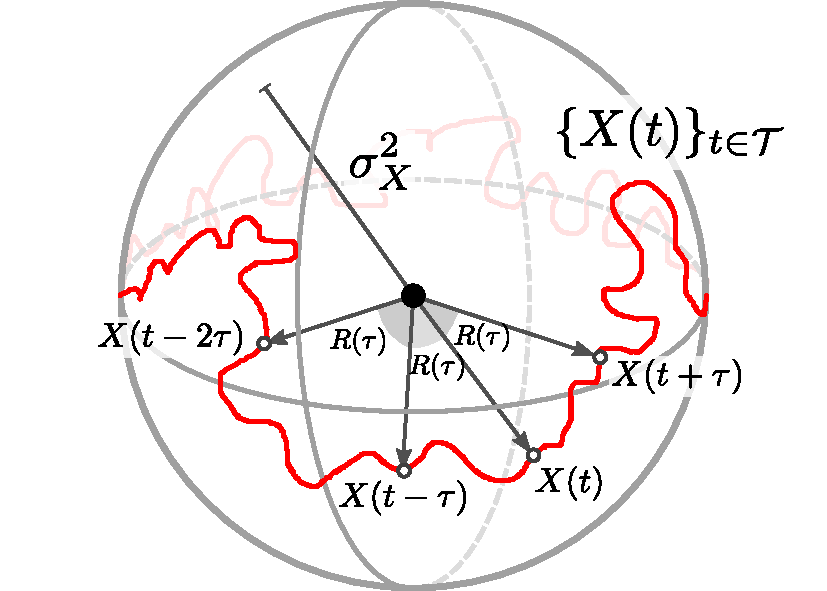
\includegraphics[width=.6\textwidth]{./img_diagramas/esfera_v1.pdf}
\caption[Topología esperada para un proceso estocástico débilmente estacionario y estocásticamente continuo \textit{dentro} del espacio de variables aleatorias con varianza finita.]{Topología esperada para un proceso estocástico débilmente estacionario y estocásticamente continuo, \xt , \textit{dentro} del conjunto de variables aleatorias con varianza finita, $\mathcal{A}$.
%
El objetivo de esta ilustración es visualizar algunos \textit{elementos} de \xt dentro del contexto de $\mathcal{A}$ como un espacio de Hilbert. Por ejemplo \xt está contenido en una esfera de radio $\sigma_X^2$ y centro en una variable aleatoria con distribución degenerada $D(0)$.}
\end{figure}

%%%%%%%%%%%%%%%%%%%%%%%%%%%%%%%%%%%%%%%%%%%%%%%%%%%%%%%%%%%%%%%%%%%%%%%%%%%%%%%%%%%%%%%%%%%%%%%%%%%
%%%%%%%%%%%%%%%%%%%%%%%%%%%%%%%%%%%%%%%%%%%%%%%%%%%%%%%%%%%%%%%%%%%%%%%%%%%%%%%%%%%%%%%%%%%%%%%%%%%

\section{Función de densidad espectral}
\label{sec:fde}

%Repitiendo el comentario expuesto en la sección \ref{lazy:fourier_stieltjes}, existe una gran cantidad de espacios para los cuales se puede definir una generalización de la transformada de Fourier.
%
%En este capítulo se considera al conjunto de procesos estocásticos estocásticamente continuos, débilmente estacionarios, de media cero y varianza finita; en concreto, se usará una forma similar a la transformada de Fourier-Stieltjes (definición \ref{lazy:fourier_stieltjes}).

Una vez definido el espacio $\mathcal{A}$ se procede a definir una primera versión del espectro de potencias; en concreto, se usará una forma similar a la transformada de Fourier-Stieltjes (definición \ref{lazy:fourier_stieltjes}).

%La forma más \textit{natural} de definir un espectro de potencias para un proceso estacionario es a través de la transformada de Fourier de sus realizaciones. 
%%
%Tal enfoque no funciona en general, pues no se puede garantizar que las realizaciones arbitrarias admitan una transformada de Fourier (ni aún de Fourier-Stieltjes).
%%
%Se define entonces el espectro en base a un límite de subcolecciones de la realización, de modo que éstas sí admitan una transformada de Fourier.

\begin{definicion}%[Función de densidad espectral, tiempo continuo]
Sea \xt un proceso estocástico en los reales, débilmente estacionario, con media 0 y varianza finita. Se define su \textbf{función de densidad espectral}, $h$, como
\begin{equation}
h(\omega) = \frac{1}{2 \pi} \lim_{T\rightarrow \infty} \E{ \abso{ \frac{1}{2T} \int_{-T}^{T} X(t) e^{-i \omega t} d\mu(t)}^{2} }
\end{equation}
con $\mu$ siendo la medida de Lebesgue si el proceso es a tiempo continuo, y la medida discreta si el proceso es a tiempo discreto.
\label{txt_FDE_cont}
\end{definicion}

%[? ejemplos: ruido rosa esta bien definido, proceso oscilatorio no esta definido, ruido blanco no esta definido]

%\begin{definicion}[Función de densidad espectral, tiempo discreto]
%Sea $\{X(t)\}_{\nicefrac{t}{\Delta_t}\in \Z}$ un proceso estacionario a tiempo discreto. Se define su {función de densidad espectral} como
%\begin{equation}
%h(\omega) = \frac{1}{2 \pi} \lim_{N\rightarrow \infty} \E{ \frac{1}{2N} 
%\abso{ \sum_{n=-N}^{N} X(n \Delta_t) e^{-i \omega n \Delta_t}}^{2} }
%\label{txt_FDE_disc}
%\end{equation}
%\end{definicion}

\begin{ejemplo}
Sea \xt el proceso oscilante descrito anteriormente.
\begin{align*}
\int_{-T}^{T} X(t) e^{-i \omega t} d\mu(t)
&= \int_{-T}^{T} \COS{t+\phi} e^{-i \omega t} dt \\
&= \int_{-T}^{T} \frac{1}{2} \left[ e^{i (t + \phi)} + e^{-i (t + \phi)} \right] e^{-i \omega t} dt \\
&= \frac{1}{2} e^{i \phi} \int_{-T}^{T} e^{-i(\omega-1)t} dt + \frac{1}{2} e^{-i \phi} \int_{-T}^{T} e^{-i(\omega+1)t} dt \\
&= \frac{1}{2} e^{i \phi} \frac{e^{-i(\omega-1)T} - e^{i(\omega-1)T}}{-i(\omega-1)} + \frac{1}{2} e^{-i \phi} \frac{e^{-i(\omega+1)T} - e^{i(\omega+1)T}}{-i(\omega+1)} \\
&= e^{i \phi} \frac{\SEN{(\omega-1)T}}{\omega-1} + e^{-i \phi} \frac{\SEN{(\omega+1)T}}{\omega+1}
\end{align*}

Luego entonces
\begin{align*}
\abso{ \frac{1}{2T} \int_{-T}^{T} X(t) e^{-i \omega t} d\mu(t)}^{2} 
&= 
\frac{1}{4}\abso{ e^{i \phi} \frac{\SEN{(\omega-1)T}}{(\omega-1)T} + e^{-i \phi} \frac{\SEN{(\omega+1)T}}{(\omega+1)T} }^2 \\
&=
\frac{1}{4}\left( \frac{\SEN{(\omega-1)T}}{(\omega-1)T} \right)^2 + \left( \frac{\SEN{(\omega+1)T}}{(\omega+1)T} \right)^2 \\
&\pheq + \frac{1}{2} \left( \frac{\SEN{(\omega-1)T}}{(\omega-1)T} \right) \left( \frac{\SEN{(\omega+1)T}}{(\omega+1)T} \right) \COS{2 \phi}
\end{align*}

De la forma relativamente simple de \xt, se deduce que
\begin{align*}
\E{ \abso{ \frac{1}{2T} \int_{-T}^{T} X(t) e^{-i \omega t} d\mu(t)}^{2} }
&=
\frac{1}{4} \left( \frac{\SEN{(\omega-1)T}}{\omega-1} \right)^2 + \frac{1}{4} \left( \frac{\SEN{(\omega+1)T}}{\omega+1} \right)^2 
\end{align*}

Si $\omega \notin \{-1,1\}$ entonces
\begin{equation}
\frac{1}{2\pi} \lim_{T\rightarrow \infty} \E{ \abso{ \frac{1}{2T} \int_{-T}^{T} X(t) e^{-i \omega t} d\mu(t)}^{2} } = 0
\end{equation}
en caso contrario vale 0, ya que $\lim_{x\rightarrow0} \frac{\SEN{x}}{x} = 1$. Entonces, la función de densidad espectral para el proceso oscilante es
\begin{equation}
h(\omega) = \begin{cases}
\nicefrac{1}{\pi} &, x \in \{ -1, 1 \} \\
0 &, \text{otro caso}
\end{cases}
\end{equation}
\end{ejemplo}

La definición \ref{txt_FDE_cont} produce información consistente con el comportamiento de los procesos, sin embargo tiene varios problemas con implicaciones prácticas.
%
Primeramente está que para calcularse requiere el valor esperado sobre todo el espacio de eventos de un proceso estocástico, lo cual en general puede ser complicado.

Con vista al ejemplo, puede decirse que la función de densidad espectral obtenida no es una función de `densidad' en el mismo sentido que una función de densidad de probabilidad.
%
Continuando con ejemplo, uno quisiera definir una función de espectro integrado, $H$, como
\begin{equation}
H(\omega_2) - H(\omega_1) = \frac{1}{2 \pi} \int_{\omega_1}^{\omega_2} h(\omega) d\omega
\end{equation}
una definición que falla con el ejemplo descrito. A continuación se presenta un teorema que establece formalmente la existencia de las funciones de espectro integrado, en concordancia con la definición \ref{txt_FDE_cont}.

%Usando que $h$ es una función simétrica tal que $\intR h(\omega) d\omega = \sigma_X^{2}$, entonces puede escribirse
%\begin{equation}
%H(\omega) = \frac{\sigma_X^{2}}{2} + \frac{1}{2 \pi} \intR \frac{e^{i \omega_1 \tau}-1}{i \tau} R(\tau) d\tau = \frac{\sigma_X^{2}}{2} + \frac{1}{2 \pi} \intR \frac{\SEN{\omega \tau}}{\tau} R(\tau) d\tau
%\end{equation}

%%%%%%%%%%%%%%%%%%%%%%%%%%%%%%%%%%%%%%%%%%%%%%%%%%%%%%%%%%%%%%%%%%%%%%%%%%%%%%%%%%%%%%%%%%%%%%%%%%%
%%%%%%%%%%%%%%%%%%%%%%%%%%%%%%%%%%%%%%%%%%%%%%%%%%%%%%%%%%%%%%%%%%%%%%%%%%%%%%%%%%%%%%%%%%%%%%%%%%%

%\section{Representación espectral}
%\label{sec:representacion}

%\begin{teorema}
%Sea \xt un proceso estocástico débilmente estacionario, de media cero y varianza finita.
%%
%Sea $h$ su función de densidad espectral y sea $R$ su función de autocovarianza. 
%%
%Entonces se cumple que
%\begin{equation}
%h(\omega) = \frac{1}{2\pi} \intR e^{i \omega \tau} R(\tau) d\tau
%\end{equation}
%\label{teo:corr_four}
%\end{teorema}
%\begin{proof}
%Usando que $h = \lim_{T\rightarrow\infty} G_T$, nótese que
%\begin{align*}
%\abso{G_T(\omega)}^{2} &= 
%\intR e^{i \omega t} \left[ \left(\frac{1}{\sqrt{2\pi}} \right)^{2} \intR X_T(u) X_T(u-\tau) du \right] d\tau \\
%&=
%\frac{1}{2\pi} \intR e^{i \omega t} \left[ \intR X_T(u) X_T(u-\tau) du \right] d\tau \\
%\end{align*}
%Esta integral puede verse como la transformada de Fourier de la función de autocorrelación de la serie truncada, $\widehat{R}_T$
%\begin{align*}
%\widehat{R}_T (\tau) &= \frac{1}{2T} \intR X_T(u) X_T(u-\tau) du \\
%&= \begin{cases}
%\frac{1}{2T} \int_{-T+\abso{\tau}}^{T} X(u) X(u-\abso{\tau}) du &, \abso{\tau} \leq T \\
%0 &, \text{otro caso}
%\end{cases}
%\end{align*}
%Así entonces
%\begin{align*}
%h(\omega) &=
%\lim_{T\rightarrow \infty} \E{\frac{1}{2T} \abso{G_T(\omega)}^{2}} \\
%&=
%\lim_{T\rightarrow \infty}
%\E{\frac{2T}{2\pi} \intR e^{i \omega t} \widehat{R}_T(\tau) d\tau }\\
%&=
%\frac{1}{2\pi}
%\lim_{T\rightarrow \infty}
%2T \intR e^{i \omega t} \E{\widehat{R}_T(\tau)} d\tau\\
%\end{align*}
%Para esto, si $\abso{\tau} \leq 2T$
%\begin{align*}
%\E{\widehat{R}_T(\tau)} &=
%\E{\frac{1}{2T} \intR X_T(u) X_T(u-\tau) du} \\
%&=
%\E{ \frac{1}{2T} \int_{-T+\abso{\tau}}^{T} X(u) X(u-\tau) du } \\
%&=
%\frac{1}{2T} \int_{-T+\abso{\tau}}^{T} \E{X(u) X(u-\tau)} du \\
%&=
%\frac{1}{2T} \int_{-T+\abso{\tau}}^{T} R(\tau) du \\
%&=
%\frac{1}{2T} \left( 1 - \frac{\abso{\tau}}{2T} \right) R(\tau)
%\end{align*}
%pero si $\abso{\tau}>2T$ entonces $\widehat{R}_T = 0$. Luego entonces
%\begin{align*}
%h(\omega) &=
%\frac{1}{2\pi} \lim_{T\rightarrow \infty}
%\int_{-T}^{T} e^{i \omega t} \left( 1 - \frac{\abso{\tau}}{2T} \right) R(\tau) d\tau\\
%&=
%\frac{1}{2\pi} \lim_{T\rightarrow \infty}
%\intR e^{i \omega t} g_T(t) R(\tau) d\tau
%\end{align*}
%con
%\begin{equation}
%g_T = \begin{cases}
%1 - \nicefrac{\abso{\tau}}{2T} &, \abso{\tau} \leq 2T \\
%0 &, \text{otro caso}
%\end{cases}
%\end{equation}
%
%Para establecer el límite anterior nótese que para cualesquiera $\tau, T$ se cumple que $0\leq g_\tau \leq 1$, entonces
%\begin{align*}
%\intR e^{i \omega t} g_T(t) R(\tau) d\tau
%&\leq
%\abso{\intR e^{i \omega t} g_T(t) R(\tau) d\tau } \\
%&\leq
%\intR \abso{g_T(\tau)} \abso{ R(\tau)} d\tau \\
%&\leq
%\intR \abso{ R(\tau)} d\tau 
%\end{align*}
%
%Para cada $\omega$, el módulo de $\int_{-T}^{T} e^{i \omega t} g_\tau(t) R(\tau) d\tau$ es monótonamente creciente y acotado, luego entonces, por el teorema de convergencia dominada de Lebesgue, se tiene que
%\begin{align*}
%h(\omega) &=
%\frac{1}{2\pi} \lim_{T\rightarrow \infty}
%\intR e^{i \omega t} g_T(t) R(\tau) d\tau\\
%&=
%\frac{1}{2\pi} 
%\intR e^{i \omega t} \left[ \lim_{T\rightarrow \infty} g_T(t) \right] R(\tau) d\tau\\
%&=
%\frac{1}{2\pi} 
%\intR e^{i \omega t} R(\tau) d\tau\\
%\end{align*}
%\end{proof}
%
%
%
%Conviene remarcar que el teorema \ref{teo:corr_four} sólo aplica si el proceso admite una función de densidad espectral, y en consecuencia no es claro si el espectro integrado queda bien definido para procesos que no admiten una densidad espectral. 
%%
%Por ejemplo, considérese el proceso $P$ definido como 
%
%El siguiente teorema permite establecer condiciones generales para las cuales se puede definir un espectro de potencias para un proceso estacionario.

\begin{teorema}[Wiener-Khintchine]
Una condición suficiente y necesaria para que $R$ sea una función de autocovarianza para algún proceso estocástico a tiempo continuo \xt débilmente estacionario y estocásticamente continuo, es que exista una función $H$ que tenga las siguientes propiedades
\begin{itemize}
\item Monótonamente creciente
\item $\lim_{\omega\rightarrow -\infty} H(\omega) = 0$
\item $\lim_{\omega\rightarrow +\infty} H(\omega) < \infty$
\end{itemize}
y tal que para todo $\tau \in \R$ se cumple que
\begin{equation*}
R(\tau) = \intR e^{i \omega \tau} dH(\omega)
\end{equation*}
Como notación, $H$ será referido como la \textbf{función de espectro integrado} para \xt.
%
Adicionalmente, si $H$ es absolutamente continua, se define a $h$, la \textbf{función de densidad espectral} como
\begin{equation}
h(\omega) d\omega := dH(\omega)
\end{equation}
\label{t_wienerkhinchin}
\end{teorema}

%Una vez definido y probada la existencia de la función de espectro integrado normalizado $dF$, se define la \textbf{función de espectro integrado} $dH$ (sin el adjetivo \textit{normalizado}) como
%$dH := \sigma_X^{2} dF$.

%%%%%%%%%%%%%%%%%%%%%%%%%%%%%%%%%%%%%%%%%%%%%%%%%%%%%%%%%%%%%%%%%%%%%%%%%%%%

\section{Representación espectral}

%Una vez establecidas las condiciones de existencia para el espectro de potencias de un proceso débilmente estacionario, una pregunta muy natural es sobre la unicidad.
%%
%Cuando se discutió la transformada de Fourier para funciones en $L^{2}$, se dejó en claro que es un operador invertible salvo por su núcleo (definición ?).

%Se mostró que la transformada de Fourier puede ser parameterizada en módulo y argumento, siendo el primero es equivalente (salvo una función invertible) al espectro.
%%
%El espectro de un proceso estacionario fue definido como
%\begin{align*}
%h(\omega) &= \lim_{T\rightarrow\infty} \E{\abso{ G_T(\omega)}^{2}} \\
%G_T(\omega) &= \int_{-T}^{T} e_{i \omega t} X(t) dt
%\end{align*}
%la componente $G_T$ cumple intuitivamente el papel de la transformada de Fourier, pero es omitida para demostrar más fácilmente la existencia del espectro $h$. Contemplando la parametrización de la transformada de Fourier, ¿puede definirse algo equivalente al argumento para un proceso estacionario?
%%
%%Un enfoque propuesto por Winer [citar, 1930, capitulo 1] es
%[? mejorar redacción]

En el teorema \ref{t_wienerkhinchin} se definió la función de densidad espectral en términos de la función de autocorrelación de un proceso.
%
Una pregunta natural es si se podría obtener la misma función en términos del proceso en sí.
%
Dicha interrogante se deriva de la pregunta sobre si el proceso puede \textit{reconstruirse} a partir de su espectro.

La respuesta, afirmativa salvo unicidad, conduce directamente a una forma de representar al proceso en base a su espectro, conocida como \textbf{representación de Wold-Cramér}.
%
Dicha representación será usada con fluidez durante el resto de este capítulo, y como una motivación fuerte para el siguiente capítulo.

\begin{teorema}
Sea \xt un proceso a tiempo continuo, débilmente estacionario, de media 0 y estocásticamente continuo en el sentido de media cuadrática. Existe un proceso ortogonal $\{Z(\omega)\}$ tal que, para todo tiempo $\omega$ admisible, se puede escribir
\begin{equation*}
X(t) = \intR e^{i t \omega} dZ(\omega)
\end{equation*}
Donde el proceso $\{Z(t)\}$ tiene las siguientes propiedades para todo $\omega$
\begin{itemize}
\item $\E{dZ(\omega)} = 0$
%\item $\E{\abso{dZ(\omega)}^{2}} = dH(\omega)$
\item $\Cov{dZ(\omega),dZ(\lambda)} = dH(\omega) \delta(\omega, \lambda)$
\end{itemize}
Donde $dH(\omega)$ el espectro integrado de \xt
\label{rep_espectral}
\end{teorema}

%\begin{proof}
%Se considera a \xt, un proceso que satisface las condiciones del teorema, y a $\{x(t)\}_{t\in \mathcal{T}}$, una realización. Se define $x_T$, una extensión periódica de la restricción de longitud $T$ para $x$, como
%%\begin{equation}
%%x_T(t) = x\left( 2T \entero{\frac{t+T}{2T}} -T \right)
%%\end{equation}
%\begin{equation}
%x_T(t) = \begin{cases}
%x(t) &, \abso{t} \leq T \\
%x(t_*+2pT) &, p \text{ tal que } \abso{t_*}\leq T
%\end{cases}
%\end{equation}
%Como $x_T$ es periódica, con periodo $2T$, puede escribirse como
%\begin{align*}
%x_T(t) &= \sum_{n=-\infty}^{\infty} A_n e^{i \nicefrac{2\pi n t }{T}} \\
%A_n &= \frac{1}{2T} \int_{-T}^{T} x_T(t) e^{-i \nicefrac{2\pi n t }{T}}
%\end{align*}
%Se define entonces una función $G_T$, análoga a la usada al definir el espectro, como
%\begin{equation}
%G_T(\omega) = \int_{-T}^{T} \frac{1}{\sqrt{2 \pi}} x_T(t) e^{i \omega t} dt = \int_{-T}^{T}     \frac{1}{\sqrt{2 \pi}} x_T(t) e^{i \omega t} dt
%\end{equation}
%Luego entonces, puede escribirse
%\begin{equation}
%asdasd
%\end{equation}
%\end{proof}

\begin{proof}
Se mostró anteriormente que $\mathcal{R}$, el conjunto de variables aleatorias con media cero y varianza finita, tiene la estructura de espacio de Hilbert con el producto interno
\begin{equation}
\langle U , V \rangle := \Cov{U,V} = \E{U, \overline{V}}
\end{equation}
Ahora bien, un proceso débilmente estacionario \xt puede verse como una \textit{curva} en $\mathcal{R}$ indexada por $t \in \mathcal{T}$.
%
Por el teorema de Wiener-Khintchine, existe un proceso ortogonal $dH$ tal que puede escribirse
\begin{equation}
\pint{X(t),X(s)} = R(t-s) = \intR e^{i \omega (t-s)} dH(\omega)
\end{equation} 
De manera más general, puede hablarse de una familia de funciones $\{ \phi_t \}_{t\in \mathcal{T}}$ (anteriormente se usó $\phi_t(\omega) = e^{i \omega t}$) y escribir
\begin{equation}
\pint{X(t),X(s)} = \intR \phi_t(\omega) \overline{\phi_s(\omega)} dH(\omega)
\end{equation} 
Usando la familia de funciones $\{ \phi_t \}_{t\in \mathcal{T}}$ puede construirse un segundo espacio de Hilbert, $\mathcal{H}_\phi$, como las combinaciones lineales de estas funciones.
A este segundo espacio se le define el producto interno
\begin{equation}
\pint{\phi_1,\phi_2}_H := \intR \phi_1(\omega) \overline{\phi_2(\omega)} dH(\omega)
\end{equation} 
Posteriormente se define un mapeo $M : \mathcal{H}_\phi \rightarrow \mathcal{R}$ como
\begin{equation}
M[\phi_t] := X(t)
\end{equation}
el cual se extiende linealmente para cualesquiera coeficientes $c_1, c_2, \cdots \in \R$ y tiempos admisibles $t_1, t_2, \cdots \in \mathcal{T}$
\begin{equation}
M\left[ \sum_i c_i \phi_{t_i} \right] = \sum_i c_i M\left[ \phi_{t_i} \right]
\end{equation}
Trivialmente, $M$ conserva productos internos; basta notar que
\begin{equation}
\pint{X(t),X(s)} = \intR \phi_1(\omega) \overline{\phi_2(\omega)} dH(\omega) = \pint{\phi_1,\phi_2}_H
\end{equation}
Ahora, para trabajar con las funciones $\phi$ conviene descomponerlas en una base más \textit{sencilla}, como límite de funciones simples. Para ello, se define una función indicadora
\begin{equation}
I(\omega; \omega_0, \omega_f) := \begin{cases}
1 &, \omega_0 \leq \omega < \omega_f \\
0 &, \text{otro caso}
\end{cases}
\end{equation}
Luego, sea $\{\omega_0, \omega_1, \cdots, \omega_N\}$ una partición del intervalo $[-n,n]$, con $n\gg N$. Entonces, en virtud del teorema de convergencia dominada de Lebesgue
\begin{equation}
\phi_t(\omega) = \lim_{n\rightarrow\infty} \sum_{i=1}^{N} I(\omega; \omega_{i-1}, \omega_i) \left[  \inf_{\omega \in [\omega_{i-1},\omega_i]} \phi_t(\omega_{i})\right]
\label{asd}
\end{equation}
Usando tal representación para las funciones $\phi$'s, se define a $Z$ como
\begin{equation}
Z(\omega_f) - Z(\omega_0) = M\left[ I(\omega; \omega_f, \omega_0) \right]
\end{equation}
Luego entonces, aplicando $M$ a ambos lados de la expresión \ref{asd} se obtiene
\begin{align*}
M\left[ \phi_t(\omega) \right] &= M\left[ \lim_{n\rightarrow\infty} \sum_{i=1}^{N} I(\omega; \omega_{i-1}, \omega_i) \left[  \inf_{\omega \in [\omega_{i-1},\omega_i]} \phi_t(\omega_{i})\right] \right] \\
&= \lim_{n\rightarrow\infty} \sum_{i=1}^{N} M\left[I(\omega; \omega_{i-1}, \omega_i) \right] \left[  \inf_{\omega \in [\omega_{i-1},\omega_i]} \phi_t(\omega_{i})\right] \\
&= \lim_{n\rightarrow\infty} \sum_{i=1}^{N} \left( Z(\omega_i) - Z(\omega_{i-1})\right) \left[  \inf_{\omega \in [\omega_{i-1},\omega_i]} \phi_t(\omega_{i})\right] \\
&= \intR \phi_t(\omega) dZ(\omega)
\end{align*}
El resultado que se busca queda establecido porque $M[\phi_t] = X(t)$
\begin{equation}
X(t) = \intR \phi_t(\omega) dZ(\omega)
\end{equation}
\end{proof}

%Es muy importante notar que en la demostración del teorema anterior se ha usado que el espacio de variables aleatorias con media cero y varianza finita, $\mathcal{A}$, se comporta como un espacio de Hilbert.
%
Cabe destacar que el uso de integrales respecto a un proceso estocástico
%; este tipo de integrales fueron 
es conforme 
%las cuales son como se usaron
%usadas 
a las usadas
en la sección \ref{sec:int_proc_est}.

Bajo el contexto de espacios de Hilbert, es muy importante notar el proceso $\{Z(t)\}_{t\in \R}$ es ortogonal, es decir que está compuesto por variables aleatorias no--correlacionadas.
%
Este hecho ayuda a interpretar de forma más \textit{natural} a $\abso{dZ}^2$ como un espectro de potencias.

\subsection{Representación de procesos a tiempo discreto}

La existencia de espectros para procesos a tiempo discreto es dada por el teorema

\begin{teorema}[Wold]
Una condición suficiente y necesaria para que $R$ sea una función de autocovarianza de 
algún proceso estocástico a tiempo discreto \xt débilmente estacionario es que exista 
una función $H$ con las siguientes propiedades
\begin{itemize}
\item Monótonamente creciente
\item $\lim_{\omega \longrightarrow -\pi} F(\omega) = 0$
\item $\lim_{\omega \longrightarrow +\pi} F(\omega) = 1$
\end{itemize}
y tal que para todo $\tau \in \R$ se cumple que
\begin{equation*}
R(\tau) = \intPI e^{i \omega \tau} dH(\omega)
\end{equation*}
\label{t_wold}
\end{teorema}

\begin{proof}
Por simplicidad, supóngase que $\Delta_X=1$. A tiempo discreto, la función de autocovarianza adquiere la forma de una secuencia $\{R(\tau)\}_{\tau\in \Z}$. Se define una función $R_C$ que es igual a $R$ pero cuyo dominio es $\R$, de la forma
\begin{equation}
R_C(\tau) = \left( 1 - \tau + \entero{\tau} \right) R\left( \entero{\tau} \right) +
\left( s - \entero{\tau} \right) R\left( \entero{\tau} +1 \right)
\end{equation}
Fue demostrado por Priestley \cite{Priestley81} que existe un proceso estacionario cuya función de autocovarianza es $R_C$, luego entonces por el teorema \ref{t_wienerkhinchin} existe una función de distribución $Q$ tal que 
\begin{equation}
R_C(\tau) = \intR e^{i \omega \tau} dQ(\omega)
\end{equation}
Dado que $R$ y $R_C$ son iguales cuando $\tau$ es entero, se puede considerar la siguiente manipulación con $\tau \in \Z$.
\begin{align*}
R(\tau) &= 
\intR e^{i \omega \tau} dQ(\omega) \\
&=
\sum_{s = -\infty}^{\infty} \int_{(2s-1)\pi}^{2s+1 \pi} e^{i \omega \tau} Q(\omega) \\
&=
\sum_{s = -\infty}^{\infty} \int_{-\pi}^{\pi} e^{i \left(\omega + 2\pi s \right) \tau} Q(\omega + 2 \pi s) \\
&=
\sum_{s = -\infty}^{\infty} \int_{-\pi}^{\pi} e^{i \omega \tau} Q(\omega + 2 \pi s) \\
&=
\int_{-\pi}^{\pi} e^{i \omega \tau} \left[ \sum_{s = -\infty}^{\infty} Q(\omega + 2 \pi s) \right] \\
\end{align*}
Finalmente se puede definir a $F$, la función de densidad descrita por el teorema, usando
\begin{equation}
dF(\omega) = \sum_{s = -\infty}^{\infty} Q(\omega + 2 \pi s)
\end{equation}
El que $F$ sea monótonamente se deduce de que $Q$ lo es. Como $dQ$ es simétrica, puede definirse convenientemente que $F(-\pi)=0$ y $F(\pi) = 1$ con base a que
\begin{equation}
F(\pi) = \intPI \left[ \sum_{s = -\infty}^{\infty} Q(\omega + 2 \pi s) \right] = \intR dQ(\omega) = 1
\end{equation}
\end{proof}

%En virtud del teorema de Wold, se puede obtener una variante del teorema \ref{rep_espectral} para procesos a tiempo discreto cambiando el intervalo de integración.

\begin{teorema}
Sea \xt un proceso a tiempo discreto, débilmente estacionario y de media 0. Existe un proceso ortogonal $\{Z(\omega)\}$ tal que, para todo tiempo $\omega$ admisible, se puede escribir
\begin{equation*}
X(t) = \intPI e^{i t \omega} dZ(\omega)
\end{equation*}
Donde el proceso $\{Z(t)\}$ tiene las siguientes propiedades para todo $\omega$
\begin{itemize}
\item $\E{dZ(\omega)} = 0$
%\item $\E{\abso{dZ(\omega)}^{2}} = dH(\omega)$
\item $\Cov{dZ(\omega),dZ(\lambda)} = dH(\omega) \delta(\omega, \lambda)$
\end{itemize}
Donde $dH(\omega)$ el espectro integrado de \xt
\label{rep_espectral2}
\end{teorema}

La demostración es completamente análoga a la del teorema \ref{rep_espectral}, reemplazando al teorema de Wiener-Khintchine por el de Wold. 
%Como notación, las representaciones en los teoremas \ref{rep_espectral} y \ref{rep_espectral2} son referidas como \textbf{representaciones de Wold-Cramér}.

%%%%%%%%%%%%%%%%%%%%%%%%%%%%%%%%%%%%%%%%%%%%%%%%%%%%%%%%%%%%%%%%%%%%%%%%%%%%%%%%%%%%%%%%%%%%%%%%%%%
%%%%%%%%%%%%%%%%%%%%%%%%%%%%%%%%%%%%%%%%%%%%%%%%%%%%%%%%%%%%%%%%%%%%%%%%%%%%%%%%%%%%%%%%%%%%%%%%%%%

\section{Efecto {alias}}

Hasta ahora se han tratado por separado los procesos a tiempo discreto y a tiempo continuo. 
%
Una vez expuestos algunos resultados importantes, se procede a explorar la familia de los procesos a tiempo discreto generados como subcolección de algún proceso a tiempo continuo. 
%
Dicha familia se vuelve importante porque se ha decidido modelar a las señales electrofisiológicas como procesos a tiempo continuo, pero sólo se pueden obtener registros de ellas a tiempo discreto.

Este tópico es relevante desde el punto de vista práctico, ya que existe una amplia variedad de condiciones técnicas bajo las cuales se suelen efectuar los registros. La AASM establece un mínimo de 128 puntos por segundo (\hz) para realizar las polisomnografías, pero la frecuencia de muestreo usualmente es decidida dependiendo del fenómeno a observar y las características del aparato de registro a usarse.
%
Siguiendo esta idea, conviene hablar del posible efecto de obtener registros con una mayor o menor cantidad de puntos por unidad de tiempo

Considérese un proceso a tiempo continuo y débilmente estacionario, \xt, y sea $\Delta_t \in \R$ arbitrario.
%
Se construye al proceso $\{Y(n)\}_{n\in \mathbb{N}}$ como
\begin{equation}
Y(n) = X(n \Delta_t)
\end{equation}

En virtud del teorema \ref{rep_espectral}, \xt admite una representación de la forma
\begin{equation}
X(t) = \intR e^{i \omega t }  dZ_X(\omega)
\end{equation}

Luego entonces puede reescribirse
\begin{align}
Y(n) &= \intR e^{i \omega n \Delta_t} dZ_X(\omega) \nonumber \\
&= \sum_{k \in \N} \int_{\nicefrac{(2k-1)\pi}{\Delta_t}}^{\nicefrac{(2k+1)\pi}{\Delta_t}}
e^{i \omega n \Delta_t} dZ_X(\omega) \nonumber \\
&= \sum_{k \in \N} \int_{-\nicefrac{\pi}{\Delta_t}}^{\nicefrac{\pi}{\Delta_t}}
e^{i \left( \omega + \frac{2 k \pi}{\Delta_t} \right) n \Delta_t}
dZ_X\left( \omega + \nicefrac{2 k \pi}{\Delta_t}\right) \nonumber \\
&= \sum_{k \in \N} \int_{-\nicefrac{\pi}{\Delta_t}}^{\nicefrac{\pi}{\Delta_t}}
e^{i \omega n \Delta_t}
dZ_X\left( \omega + \nicefrac{2 k \pi}{\Delta_t}\right)
\end{align}

Con base a lo anterior, puede definirse para 
$\omega \in \left[ -\nicefrac{\pi}{\Delta_t} , \nicefrac{\pi}{\Delta_t} \right]$
\begin{equation}
dZ_Y(\omega) := \sum_{k \in \N} dZ_X\left( \omega + \nicefrac{2 k \pi}{\Delta_t}\right)
\end{equation}

En base al teorema \ref{rep_espectral}, se define para 
$\abso{\omega} \leq \nicefrac{\pi}{\Delta_t}$
\begin{align}
dH_Y(\omega) &= \E{\abso{dZ_Y(\omega)}^{2}} \nonumber \\
&= \E{\abso{\sum_{k \in \N} dZ_X\left( \omega + \nicefrac{2 k \pi}{\Delta_t}\right)}^{2}}
\nonumber \\
&= \sum_{k \in \N} \E{\abso{dZ_X\left( \omega + \nicefrac{2 k \pi}{\Delta_t}\right)}^{2}}
\nonumber \\
&= \sum_{k \in \N} dH_X\left( \omega + \nicefrac{2 k \pi}{\Delta_t}\right)
\end{align}

En el segundo paso se usa que $\{ dZ_X \}$ es un proceso ortogonal de media cero. Antes de poder declara que $dH_Y$ es el espectro integrado del proceso discretizado,conviene hacer el cambio de variable $\wdd := \omega \Delta_t$
\begin{align*}
dH_Y(\wdd) &= dH_Y(\omega \Delta_t) \frac{d\wdd}{d\omega} \\
&= \frac{1}{\Delta_t} dH_Y(\omega \Delta_t)
\end{align*}
donde $\abso{\wdd} \leq \pi$.
%
Si \xt posee un espectro puramente continuo --de manera equivalentemente, si $dH_X$ es absolutamente continua-- entonces puede escribirse
\begin{equation}
h_Y(\wdd) = \frac{1}{\Delta_t} \sum_{k \in \N} h_X\left( \omega + \nicefrac{2 k \pi}{\Delta_t}\right)
\end{equation}
con $\abso{\omega} \leq \pi$. 
%
Así entonces $h_Y$ puede entenderse como una versión \textit{colapsada} de $h_X$, fenómeno conocido como \textbf{efecto alias}.

%%%%%%%%%%%%%%%%%%%%%%%%%%%%%%%%%%%%%%%%%%%%%%%%%%%%%%%%%%%%%%%%%%%%%%%%%%%%%%%%%%%%%%%%%%%%%%%%%%%

\section{Filtros lineales}
\label{sec:lazy_filtros}

\begin{definicion}
Se dice que un operador $\mathcal{L}_g : L^{2} \rightarrow L^{2}$ es un \textbf{filtro lineal} si puede escribirse de la forma
\begin{equation}
\mathcal{L}_g[f] = \intR g(u) f(t-u) du
\end{equation}
para alguna función $g\in L^{2}$ que es referida como \textbf{función de respuesta}.
\end{definicion}

Naturalmente, los filtros lineales son funciones lineales. 
%
Son continuos en la identidad aditiva de $L^{2}$, y por tanto son continuos en todo $L^{2}$. 
%
Como los filtros lineales son funciones lineales y continuas, entonces son funciones medibles bajo la medida de Lebesgue. 
%
Se puede hablar de la composición de un filtro lineal $\mathcal{L}_g$ con un proceso estocástico \xt, es decir, definir un proceso de la forma
\begin{equation}
Y(t) = \mathcal{L}_g[X](t) =  \intR g(u) X(t-u) du
\label{eq:filtrado}
\end{equation}

Los procesos generados como en \ref{eq:filtrado}, usualmente referidos como \textit{procesos filtrados}, son comunes en el análisis de señales. 
%
En este trabajo serán usados para construir estimadores consistentes para el espectro de potencias.
%
Para ello, conviene describir la relación entre el espectro de un proceso y el de su \textit{versión filtrada}.

\begin{teorema}
Sea \xt un proceso a tiempo continuo, estocásticamente continuo, débilmente estacionario, de media cero y varianza finita; sea $H_X$ su función de espectro integrado.
%
Sea $\mathcal{L}_g$ un filtro lineal, con $g$ su función de respuesta.
%
Defínase al proceso $\{Y(t)\}_{t\in \mathcal{T}}$ como
\begin{equation}
Y(t) = \mathcal{L}_g[X](t) =  \intR g(u) X(t-u) du
\end{equation}

Entonces $H_Y$, la función de espectro integrado de $\{Y(t)\}_{t\in \mathcal{T}}$, satisface
\begin{equation}
dH_Y(\omega) = \abso{\Gamma(\omega)}^{2} dH_X(\omega)
\end{equation}
donde $\Gamma(\omega) := \intR g(u) e^{i (\omega -u) } du$ será referida como la \textbf{función de transferencia} asociada a $\mathcal{L}_g$. 
\label{lazy:rel_espectros}
\end{teorema}

\begin{proof}
Usando el teorema \ref{rep_espectral}, para \xt puede escribirse
\begin{equation}
X(t) = \intR e^{i \omega t }  dZ_X(\omega)
\end{equation}

Análogamente para $\{Y(t)\}_{n\in \mathbb{N}}$
\begin{align*}
Y(t) &= \intR g(u) X(t-u) du \\
&= \intR g(u) \left[ \intR e^{i \omega (t-u) }  dZ_X(\omega) \right] du \\
&= \intR e^{i \omega t } \left[ \intR g(u) e^{i \omega -u } du \right] dZ_X(\omega) \\
&= \intR e^{i \omega t } \Gamma(\omega) dZ_X(\omega)
\end{align*}
%donde $\Gamma(\omega) = \intR g(u) e^{i \omega -u } du$ será referida como la \textbf{función de transferencia} asociada al filtro. 
%
Luego entonces
\begin{align*}
dH_Y(\omega) &= \E{\abso{dZ_Y(\omega)}^{2}}  \\
&= \E{\abso{\Gamma(\omega) dZ_X(\omega)}^{2}}  \\
&= \abso{\Gamma(\omega)}^{2} dH_X(\omega)
\end{align*}

Más aún, si \xt admite una función de densidad espectral $h_X$, entonces $\{Y(t)\}_{t\in \mathcal{T}}$ también, y ambos satisfacen
%
%Se concluye que si ambos procesos tengan FDE bien definidas, se cumple que
\begin{equation}
h_Y(\omega) = \abso{\Gamma(\omega)}^{2} h_X(\omega)
\label{rel:espectros}
\end{equation}
\end{proof}

Conviene notar que el teorema anterior era de esperarse como una generalización del teorema \ref{teo:convolucion}; ésto considerando que la función de transferencia es la transformada generalizada de Fourier para la función de respuesta, y que $h_X, h_Y$ son --en cierto sentido-- los módulos de las transformadas de Fourier para los procesos.

\subsection{Filtros de banda}

Como se mencionó, los filtros lineales tienen múltiples aplicaciones en el análisis de señales, además de la estimación del espectro de potencias.
%
Conviene destacar, aún como comentario, la familia de filtros lineales cuya función de transferencia es de la forma
\begin{equation}
\Gamma_{\omega_0}^{\star} (\omega) = \begin{cases}
1 &, \abso{\omega} \leq \omega_0 \\
0 &, \text{otro caso}
\end{cases}
\end{equation}
este tipo de filtros son referidos como \textit{filtros pasa bajas}.
%
Análogamente, un \textit{filtro pasa altas} tiene una la misma forma cambiando la condición por $\abso{\omega} \geq \omega_0$.
%
Los \textit{filtros pasa bandas} combina un filtro pasa bajas con $\omega_f$ y un filtro pasa bajas en $\omega_0 < \omega_f$.

De manera concreta, en base al teorema \ref{lazy:rel_espectros} puede construirse un filtro lineal $\mathcal{L}$ cuya función de transferencia sea $\Gamma_{\omega_0}^{\star}$.
%
%La función de respuesta para $\mathcal{L}$, es
%\begin{equation}
%g(t) = \frac{\SEN{\omega_0 t}}{t}
%\end{equation}

\begin{ejemplo}
Sea $\mathcal{L}$ un filtro pasa bandas con $\omega_0 = 7, \omega_f = 10$. 
%
La función de respuesta para $\mathcal{L}$ es
\begin{equation}
g(t) = \frac{\SEN{10 \pi t}}{t} - \frac{\SEN{7 \pi t}}{t}
\end{equation}
y su función de transferencia es
\begin{equation}
\Gamma(\omega) = \begin{cases}
1 &, 7 \leq \omega \leq 10 \\
0 &, \text{otro caso}
\end{cases}
\end{equation}

Se construye al proceso $\{Y(t)\}_{t\in \mathcal{T}}$ en la expresión \ref{eq:filtrado}, aplicando el filtro $\mathcal{L}$ a un proceso ruido blanco.
%
En virtud del teorema \ref{rel:espectros} la función de densidad espectral para $\{Y(t)\}_{t\in \mathcal{T}}$ es $\Gamma$, y su función de autocovarianza es $g$.

Este proceso será usado en ejemplos posteriores, así que será denominado `proceso tipo alfa' para facilitar la referencia; el nombre se debe a la analogía con las ondas cerebrales alfa, como se describen en la sección \ref{sec:eeg}.
%
En la figura \ref{img:proceso_alfa} se ilustra la apariencia de este proceso, su función de covarianza y su función de densidad espectral.
\label{lazy:proceso_alfa}
\end{ejemplo}

\begin{figure}
\centering
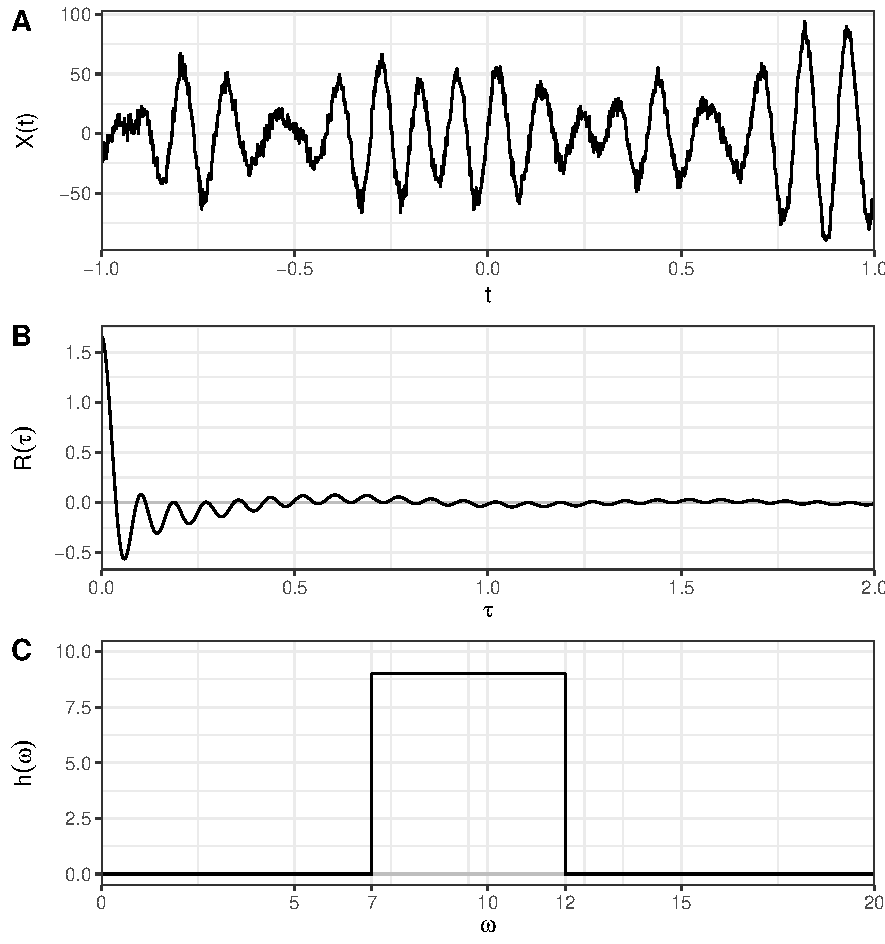
\includegraphics[width=\linewidth]{./img_mas_ejemplos/proceso_alfa.pdf}
\caption[Apariencia del proceso tipo alfa]{Apariencia del proceso tipo alfa, descrito en el ejemplo \ref{lazy:proceso_alfa}. \textbf{A.} Una realización del proceso, $H$, construida a partir de una realización del proceso ruido blanco. \textbf{B.} Función de autocorrelación, $R$, construida analíticamente. \textbf{C.} Función de densidad espectral, $h$, construida analíticamente.}
\label{img:proceso_alfa}
\end{figure}

El efecto de un filtro pasa bajas suele interpretarse como la \textit{eliminación} de los \textit{componentes de frecuencia} mayores a $\omega_0$. 
%
Tal efecto es deseable si, por ejemplo, se desea estudiar la eléctrica en el lóbulo frontal de la corteza cerebral, pero se espera interferencia por la actividad muscular en el rostro\footnote{Para una explicación completa ver la sección \ref{capitulo:psg}.}.
%
Para este fin, es conveniente usar un filtro pasa bajas con $\omega_0 = $ 100 \hz, que es la frecuencia típica de la actividad muscular.
%
%Este tipo de pre-procesamiento garantiza, por ejemplo, que en los registros no hay ruido inducido por la corriente eléctrica (120 \hz); 
%
En general, el uso de estos filtros garantiza heurísticamente la eliminación de una variedad de ruidos (señales que son registradas incidentalmente, pero no son de interés) como la corriente eléctrica o la actividad muscular.

En el presente texto no se exploran con más detalles este tipo de filtros y sus efectos; el lector interesado puede dirigirse al libro \textit{``Medical {I}nstrumentation. {A}pplications and {D}esign"} por John G. Webster \cite{Webster}.

%%%%%%%%%%%%%%%%%%%%%%%%%%%%%%%%%%%%%%%%%%%%%%%%%%%%%%%%%%%%%%%%%%%%%%%%%%%%%%%%%%%%%%%%%%%%%%%%%%%
%%%%%%%%%%%%%%%%%%%%%%%%%%%%%%%%%%%%%%%%%%%%%%%%%%%%%%%%%%%%%%%%%%%%%%%%%%%%%%%%%%%%%%%%%%%%%%%%%%%

\section{Estimadores}
\label{sec:estimadores}

%El objetivo de esta sección es calcular el espectro de potencias de un proceso a partir de una realización del mismo; en el contexto del presente trabajo, las palabras \textit{observación} y \textit{registro} serán usadas como sinónimos.
%
%Con vista en la expresión \ref{txt_FDE_cont}, un estimador \textit{natural} para el espectro sería el \textit{periodograma}.

\begin{definicion}
Sea \xt un proceso débilmente estacionario a tiempo discreto, que admite una función de densidad espectral y cuya frecuencia de muestreo es $\Delta_X=1$. Sea \xtd una realización de longitud $N$. 
%
El \textbf{periodograma}, $I_N$, es un estimador 
%para el espectro 
definido como
\begin{equation}
I_N(\omega) = \frac{1}{N} \abso{\sum_{t = 0}^{N} e^{i \omega t} x(t)}^{2}
\end{equation}
\label{txt_periodograma}
\end{definicion}

Con vista en la definición \ref{txt_FDE_cont}, el periodograma es un estimador muy \textit{natural} para dicha función.
% un estimador \textit{natural} para el espectro sería el \textit{periodograma}.
%
Conviene explorar su propiedades estadísticas que, lamentablemente, no son enteramente satisfactorias.

\begin{proposicion}
Sea \xt un proceso débilmente estacionario a tiempo discreto que admite una función de densidad espectral $h$.
%
El periodograma, $I_N$, es un estimador insesgado para $h$.
%\begin{equation}
%\E{I_N(\omega)} = h(\omega)
%\end{equation}
\end{proposicion}

\begin{proposicion}
La familia de estimadores $\{I_N\}_{N\in\N}$ satisface que
\begin{equation}
\lim_{N\rightarrow \infty} \Var{I_N(\omega)} = \left[ h(\omega) \right]^{2}
\end{equation}
\label{lazy-algo}
\end{proposicion}

%Para poder estudiar mejor al periodograma conviene escribirlo como
%\begin{align*}
%I_N(\omega) &= \frac{1}{N} \abso{\sum_{t = 0}^{N} e^{i \omega t} x(t)}^{2} \\
%&= \frac{1}{N} \left( \sum_{t = 0}^{N} e^{i \omega t} x(t) \right)
%\overline{ \left( \sum_{t = 0}^{N} e^{i \omega t} x(t) \right) } \\
%&= \frac{1}{N} \left( \sum_{t = 0}^{N} e^{i \omega t} x(t) \right)
%\left( \sum_{t = 0}^{N} e^{-i \omega t} x(t) \right) \\
%&= \frac{1}{N} \sum_{n = 0}^{N}
%x(n)^{2} \\
%&\phantom{=}
%+ \frac{1}{N} \sum_{\tau = -N}^{-1} \sum_{n = 0}^{N+\tau}
%x(n)x(n-\tau) e^{i \omega \tau} \\
%&\phantom{=}
%+ \frac{1}{N} \sum_{\tau = 1}^{N} \sum_{n = \tau}^{N}
%x(n)x(n-\tau) e^{i \omega \tau} \\
%\end{align*}

%Se puede demostrar que $\E{I_N(\omega)} = h(\omega)$, de modo que es un estimador 
%\textbf{insesgado}. Sin embargo, también se demuestra que
%\begin{equation*}
%\lim_{N\rightarrow \infty} \Var{I_N(\omega)} = \left( h(\omega) \right)^{2}
%\end{equation*}
%de modo que es un estimador \textbf{inconsistente}, lo cual lo descalifica para usarse en la 
%práctica.
%
Para entender por qué el periodograma es inconsistente, conviene escribirlo como
\begin{equation}
I_N(\omega) = 2 \sum_{\tau = -(N-1)}^{N-1} \widehat{R}^{\star}(\tau) \COS{\omega \tau}
\label{txt_periodograma2}
\end{equation}
%
donde $\widehat{R}^{\star}$ es un estimador para la función de autocovarianza, $R$, definido como
\begin{equation}
\widehat{R}^{\star} (\tau) = \frac{1}{N} \sum_{t = 1}^{N-\abso{\tau}} x(t) x(t+\abso{\tau})
\end{equation}

Así mismo, la misma expresión puede interpretarse como que el periodograma es una suma ponderada de 
los valores de $\widehat{R}^{\star}$; mientras más grande es $\tau$, menos parejas de puntos cuya 
distancia es $\tau$, y entonces $\widehat{R}^{\star}$ tiene mayor varianza cuanto mayor sea $\tau$. 

Dado que la inconsistencia del periodograma es porque el periodograma es construido usando 
estimadores con varianza elevada, la solución natural es evitar tales componentes. Para ello, 
escójase una función de pesos, $g: \R \rightarrow \R$, defínase
%
\begin{equation}
\widehat{h}(\omega) = \frac{1}{2 \pi} \sum_{\tau = -(N-1)}^{N-1} g(\tau) \widehat{R}^{\star}(\tau) 
e^{i \omega \tau} 
\label{txt_estimador}
\end{equation}

Resulta ilustrativo reescribir a $\widehat{h}$ en términos del periodograma
\begin{equation*}
\widehat{h}(\omega) = \frac{1}{2 \pi} \intPI I_N(\theta) \Gamma(\omega - \theta) d\theta
\end{equation*}
donde $\Gamma(\omega) = \intR g(u) e^{i \omega -u } du$.
%
Se puede demostrar que este tipo de estimadores son asintóticamente insesgado y consistentes.

\begin{table}
\caption{Ejemplos de funciones ventana (función de respuesta)}
\centering
\begin{small}
\begin{tabular}{lll}
\toprule
Nombre & $k(u), \abso{u} \leq \pi$ & Bosquejo \\
\midrule
Bartlett &
$\displaystyle 
1 
$
& 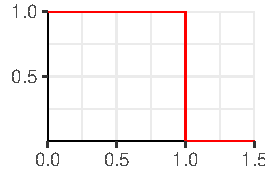
\includegraphics[scale=.4]{./img_ventanas/ventana_bartlett.pdf}\\
\rowcolor{gris}
Fejer &
$\displaystyle 
1-\abso{u}
$
& 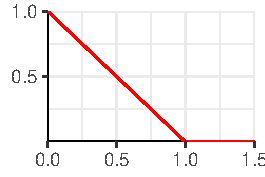
\includegraphics[scale=.4]{./img_ventanas/ventana_fejer.pdf} \\
Daniell &
$\displaystyle 
\frac{\SEN{\pi u}}{\pi u}
$
& 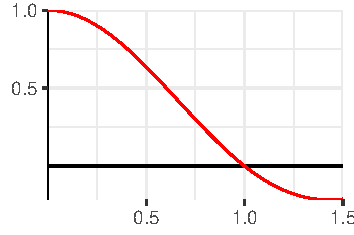
\includegraphics[scale=.4]{./img_ventanas/ventana_daniell.pdf} \\
\rowcolor{gris}
Bartlett-Priestley &
$\displaystyle 
\frac{3}{(\pi u)^{2}} \left[ \frac{\SEN{\pi u}}{\pi u} - \COS{\pi u} \right]
$
& 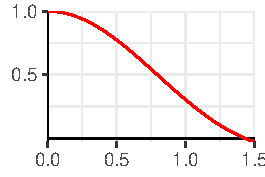
\includegraphics[scale=.4]{./img_ventanas/ventana_bartlet_priestley.pdf} \\
Cosenoidal &
$\displaystyle 
\COS{\pi u}
$
& 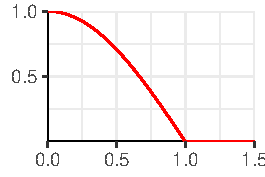
\includegraphics[scale=.4]{./img_ventanas/ventana_cosenoidal.pdf} \\
%\bottomrulec
\bottomrule
\end{tabular}
\end{small}
\label{ventanas}
\end{table}

\begin{table}
\caption{Ejemplos de funciones ventana (función de transferencia)}
\centering
\begin{small}
\begin{tabular}{lll}
\toprule
Nombre & $K(\theta)$ & Bosquejo \\
\midrule
Bartlett &
$\displaystyle 
\frac{1}{\pi} \frac{\SEN{\theta}}{\theta}
$
& 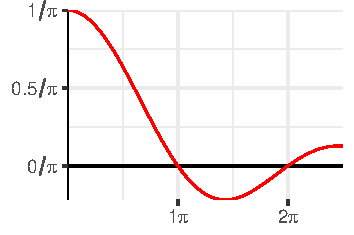
\includegraphics[scale=.4]{./img_ventanas/ventana_2_bartlett.pdf} \\
\rowcolor{gris}
Fejer &
$\displaystyle 
\frac{1}{2\pi} \left[ \frac{\SEN{\nicefrac{\theta}{2}}}{\nicefrac{\theta}{2}} \right]^{2}
$
& 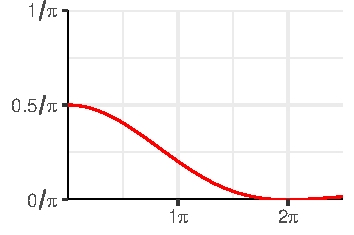
\includegraphics[scale=.4]{./img_ventanas/ventana_2_fejer.pdf} \\
Daniell &
$
\displaystyle 
\nicefrac{1}{2\pi} \text{, si } \abso{\theta}\leq \pi
$
& 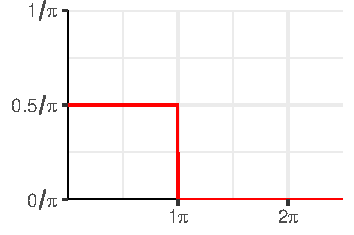
\includegraphics[scale=.4]{./img_ventanas/ventana_2_daniell.pdf} \\
\rowcolor{gris}
Bartlett-Priestley &
$\displaystyle 
\frac{3}{4 \pi} \left[ 1 - \left( \nicefrac{\theta}{\pi} \right) \right]
\text{, si } \abso{\theta}\leq \pi
$
& 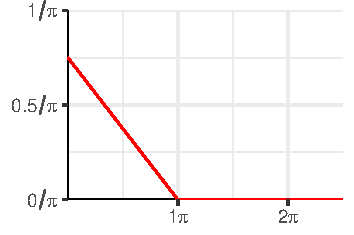
\includegraphics[scale=.4]{./img_ventanas/ventana_2_bartlet_priestley.pdf} \\
Cosenoidal &
$\displaystyle 
d
$
& 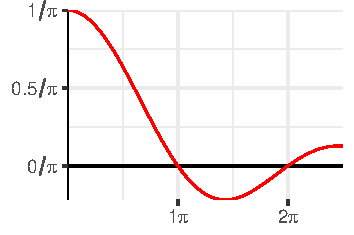
\includegraphics[scale=.4]{./img_ventanas/ventana_2_bartlett.pdf} \\
\bottomrule
\end{tabular}
\end{small}
\end{table}

%%%%%%%%%%%%%%%%%%%%%%%%%%%%%%%%%%%%%%%%%%%%%%%%%%%%%%%%%%%%%%%%%%%%%%%%%%%%%%%%%%%%%%%%%%%%%%%%%%%
%%%%%%%%%%%%%%%%%%%%%%%%%%%%%%%%%%%%%%%%%%%%%%%%%%%%%%%%%%%%%%%%%%%%%%%%%%%%%%%%%%%%%%%%%%%%%%%%%%%
%%%%%%%%%%%%%%%%%%%%%%%%%%%%%%%%%%%%%%%%%%%%%%%%%%%%%%%%%%%%%%%%%%%%%%%%%%%%%%%%%%%%%%%%%%%%%%%%%%%
%%%%%%%%%%%%%%%%%%%%%%%%%%%%%%%%%%%%%%%%%%%%%%%%%%%%%%%%%%%%%%%%%%%%%%%%%%%%%%%%%%%%%%%%%%%%%%%%%%%

%%%%%%%%%%%%%%%%%%%%%%%%%%%%%%%%%%%%%%%%%%%%%%%%%%%%%%%%%%%%%%%%%%%%%%%%%%%%%%%%%%%%%%%%%%%%%%%%%%%
%%%%%%%%%%%%%%%%%%%%%%%%%%%%%%%%%%%%%%%%%%%%%%%%%%%%%%%%%%%%%%%%%%%%%%%%%%%%%%%%%%%%%%%%%%%%%%%%%%%
%%%%%%%%%%%%%%%%%%%%%%%%%%%%%%%%%%%%%%%%%%%%%%%%%%%%%%%%%%%%%%%%%%%%%%%%%%%%%%%%%%%%%%%%%%%%%%%%%%%
%%%%%%%%%%%%%%%%%%%%%%%%%%%%%%%%%%%%%%%%%%%%%%%%%%%%%%%%%%%%%%%%%%%%%%%%%%%%%%%%%%%%%%%%%%%%%%%%%%%

\chapter{Espectro evolutivo}
\label{capitulo:espectro_evo}

El espectro evolutivo es una generalización para espectro de potencias (definido a detalle en el capítulo anterior) pero para procesos estocásticos que no son débilmente estacionarios.
% cabe destacar que la definición está influida fuertemente por el objetivo de estimación.
%
Se usa la definición tal cual fue presentada por Maurice B. Priestley en la década de 1960 \cite{Priestley65,Priestley66,Priestley69};
%
para el lector interesado en el tema es igualmente recomendable el libro \textit{``Spectral Analysis and Time Series"} del mismo autor \cite{Priestley81}, particularmente el capítulo 11.

En cuanto a estructura, este capítulo se compone de 3 secciones dedicadas únicamente al espectro evolutivo --definirlo, dar condiciones para estimarlo, construir estimadores consistentes-- y otras dos sobre las implicaciones de la estacionariedad sobre el espectro evolutivo.

Conviene destacar de manera especial que el espectro evolutivo de un proceso débilmente estacionario es equivalente a su espectro de potencias (teorema \ref{lazy:redux}). Este hecho es \textit{usado} en la sección \ref{sec:psr} para construir un \textit{detector} de estacionariedad débil: la prueba de estacionariedad débil de Priestley y Subba Rao.
%
La construcción de dicha prueba, así como su uso en registros electrofisiológicos, constituyen el punto central del presente trabajo.

%Es importante mencionar que la sección \ref{sec:espectro} representa la parte central de este capítulo, describiendo un objeto matemático bien definido que lidia con un problema que roza la vaguedad; es por ello que viene acompañado de una discusión que podría ser omitida dentro del contexto global del trabajo, pero que tiene repercusiones importantes en el uso práctico del espectro evolutivo.
%
%Por ejemplo, en la sección \ref{sec:estimacion} se discute sobre las condiciones bajo las cuales es \textit{posible} estimar el espectro evolutivo del proceso, mientras que la sección \ref{sec:doble_ventana} parte de tales condiciones para describir cómo efectuar la estimación.

%Finalmente, en la sección \ref{sec:psr} se describe una aplicación aparentemente menor del espectro evolutivo, pero que constituye una parte central en el presente trabajo: la detección de estacionariedad débil a partir del espectro evolutivo.

%%%%%%%%%%%%%%%%%%%%%%%%%%%%%%%%%%%%%%%%%%%%%%%%%%%%%%%%%%%%%%%%%%%%%%%%%%%%%%%%%%%%%%%%%%%%%%%%%%%
%%%%%%%%%%%%%%%%%%%%%%%%%%%%%%%%%%%%%%%%%%%%%%%%%%%%%%%%%%%%%%%%%%%%%%%%%%%%%%%%%%%%%%%%%%%%%%%%%%%

\section{Definición de espectro evolutivo}
\label{sec:espectro}

La idea de un espectro de potencias que cambia en el tiempo, lo que sea que eso signifique, implica una gran cantidad de problemas teóricos con implicaciones prácticas.
%
Como motivación, lo mínimo que se espera de un espectro cambiante en el tiempo, es que posea las características importantes del espectro de potencias.

La existencia del espectro de potencias es garantizada por los teoremas de Wiener-Khintchine y de Wold (teoremas \ref{t_wienerkhinchin} y \ref{t_wold}) para los procesos estocásticos débilmente estacionarios, estocásticamente continuos, con media 0 y varianza finita.
%
En ambos teoremas se establece que el espectro integrado, $H$, cumple la ecuación
\begin{equation}
R(\tau) = \int_\Omega e^{i \omega \tau} dH(\omega)
\label{lazy1}
\end{equation}
donde $R$ es la función de autocorrelación del proceso, y $\Omega$ es $\R$ o $[-\pi,\pi]$ dependiendo si el proceso es a tiempo continuo o a tiempo discreto.

Con vista a ambos teoremas, de aquí en adelante únicamente serán considerados los procesos estocásticos de media 0, varianza finita y estocásticamente continuos --aunque no necesariamente sean débilmente estacionarios.

\begin{definicion}
Sea \xt un proceso estocástico en los reales. Su \textbf{núcleo de covarianza} se define, para cualesquiera tiempos admisibles $t,s\in\mathcal{T}$, como
\begin{equation}
R(s,t) := \E{\overline{\left( X(t)-\E{X(t)} \right)}\left( X(s)-\E{X(s)} \right)}
\end{equation}
\label{s6:kernel}
\end{definicion}

La letra $R$ será usada para denotar al núcleo de covarianza siempre y cuando no haya confusión con la función de autocovarianza. 
%
Bajo esta línea de pensamiento, 
%una condición necesaria para que un proceso estocástico sea débilmente estacionario es que su función de autocovarianza $\R_A$ pueda escribirse como
%\begin{equation}
%R_A(\tau) = R(t,t\pm\tau)
%\end{equation}
%para cualquier tiempo admisible $t\in \mathcal{T}$.
%
la ecuación \ref{lazy1} puede escribirse como
\begin{equation}
R(s,t) = \intR \overline{\phi(\omega;s)}\phi(\omega;t) d\mu(\omega)
\label{s6:erre}
\end{equation}
donde se ha usado $\phi(\omega; t) = e^{i \omega t}$ y $\mu = H$, por generalidad.
%
La motivación para usar funciones $\phi$'s diferentes a las exponenciales complejas, es en principio por incertidumbre y generalidad.
%
Conviene mencionar que en la demostración del teorema de Wiener-Khintchine quedó claro que el espectro puede ser definido usando otras familias de funciones.

Con vista en la expresión \ref{s6:erre}, parece conveniente pensar en los proceso estocásticos que admitan una representación similar para alguna familia de funciones $\ef = \left\{ \phi: \R \times \mathcal{T} \rightarrow \C \right\}$. 
%
Dado que únicamente se están considerando procesos estocásticos de varianza finita, 
%en base al teorema ??,  
%por lo que 
se
pondrá como condición que cada $\phi(\bullet;t) \in \ef$ satisfaga
\begin{equation}
\intR \phi^{2}(\omega;t) d\mu(\omega) < \infty
\end{equation}

\begin{ejemplo}
Sea \xtin{\R} un proceso de Wiener, el cual se sabe que no es débilmente estacionario.
%
Como se mostró anteriormente, su núcleo de covarianza es de la forma
\begin{equation}
R(t,s) = \min \{ t , s \}
\end{equation}

Considérese a la familia de funciones $\ef = \left\{ \phi: \R \times \mathcal{T} \rightarrow \C \right\}$, definidas como
\begin{equation}
\phi(\omega; t) = \begin{cases}
1 &, 0 \leq \omega \leq t \\
0 &, \text{otro caso}
\end{cases}
\end{equation}

No es difícil verificar que $R(s,t) = \intR \overline{\phi(\omega;s)}\phi(\omega;t) d\mu_L(\omega)$, con $\mu_L$ la medida de Lebesgue.
%
Intuitivamente, la familia $\ef$ no tiene las mismas propiedades que la base de Fourier; este comentario será formalizado a continuación.
\end{ejemplo}

%Se pondrán condiciones a $\ef$ para que la expresión \ref{s6:erre} sea un tipo de espectro.

%\begin{equation}
%R(s,t) = \intR e^{i \omega (t-s)} dH(\omega)
%
%\end{equation}
%%
%donde $H$ es el espectro integrado del proceso y tiene las propiedades de una función de distribución sobre $\R$.
%%
%Como consecuencia, \xtin{\R} admite una representación de la forma
%\begin{equation}
%X(t) = \intR e^{i\omega t} dZ(\omega)
%\end{equation}
%%
%donde $Z$ es un proceso estocástico que satisface
%\begin{equation}
%\Cov{dZ(\omega_1),dZ(\omega_2)} = dH(\omega_1) \delta(\omega_1, \omega_2)
%\end{equation}

%En general, se espera tener una generalización que conserve las propiedades anteriores. Con vista a la ecuación \ref{s6:kernel}, puede restringirse la atención a procesos no-estacionarios que acepten una representación de la forma
%\begin{equation}
%R(s,t) = \intR \overline{\phi(\omega;s)}\phi(\omega;t) d\mu(\omega)
%\label{s6:erre}
%\end{equation}
%
%Para alguna medida $\mu$ definida en $\R$ y alguna familia de funciones 
%$\ef = \left\{ \phi: \R \times \mathcal{T} \rightarrow \C \right\}$; debido a la interpretación que 
%se le va a dar a este tipo de funciones, la variable $t\in \ef$ será referida como un índice.
%%
%Una condición a satisfacer es que $\Var{X^{2}(t)} = R(t,t) < \infty$, para lo cual cada 
%$\phi \in \ef$ debe ser cuadrado integrable con respecto a $\mu$, es decir
%\begin{equation}
%\intR \phi^{2}(\omega;t) d\mu(\omega) < \infty
%\end{equation}

%Se puede demostrar t(4.11.12) que bajo estas condiciones el proceso \xt acepta una representación de la forma 
%\begin{equation}
%X(t) = \intR \phi(\omega;t) dZ(\omega)
%\label{s6:representacion}
%\end{equation}
%donde el proceso $Z$ satisface que
%\begin{equation}
%\Cov{dZ(\omega_1),dZ(\omega_2)} = \mu(\omega_1) \delta(\omega_1, \omega_2)
%\end{equation}

%Se puede demostrar p(parzen 1959) que si un proceso admite una representación de la forma \ref{s6:representacion} para alguna familia de funciones $\ef$, entonces tiene admite múltiples representaciones usando diferentes familias de funciones.

%Para dar a estas representaciones la interpretación de espectro, conviene usar una familia de funciones que conserve algunas propiedades de los senos y cosenos; por ejemplo, las funciones oscilatorias

\begin{definicion}
Una función $\phi: \R \rightarrow \C$ se dice \textbf{oscilatoria} si admite una representación de la forma
\begin{equation}
\phi(t) = A(t) e^{i \omega t} 
\end{equation}
donde $A$ es de la forma
\begin{equation}
A(t) = \intR e^{i \omega t} dK(\omega)
\label{lazy2}
\end{equation}
y donde $\abso{dK(\omega)}$ tiene un único máximo global en $\omega = 0$.
\label{oscilatorio}
\end{definicion}

\begin{ejemplo}
La función $\phi(t) = e^{i \omega t}$ es oscilatoria. 
%
Basta considerar $A \equiv 1$, la cual puede expresarse como en la expresión \ref{lazy2} usando \begin{equation}
K(\omega) = \begin{cases}
1 &, 0 \leq \omega \\
0 &, \text{otro caso}
\end{cases}
\end{equation}
donde $\abso{dK}$ tiene un máximo en 0. Conviene notar que, en principio, puede expresarse a $\phi$ de forma alternativa como
\begin{equation}
\phi(t) = e^{i \lambda t} e^{i (\omega-\lambda) t}
\end{equation} 
en este caso $A_2(t) = e^{i \lambda t}$, la cual tiene una representación de la forma \ref{lazy2} usando
\begin{equation}
K_2(\omega) = \begin{cases}
1 &, \lambda \leq \omega \\
0 &, \text{otro caso}
\end{cases}
\end{equation}
la cual no tiene un máximo global en $\omega=0$.
%
La condición del máximo global indica que $A$ no es \textit{predominantemente} una función cosenoidal, sino que sólo \textit{`modula'} a $\phi$.
\label{ejemplo:sen_cos_oscilatorios}
\end{ejemplo}

\begin{ejemplo}
La función $\phi(t) = e^{i \omega t} e^{-\abso{t}}$ es oscilatoria, usando $A(t) = e^{-\abso{t}}$.
% 
Para ello, $A$ puede escribirse en la forma \ref{lazy2} con 
\begin{equation}
K(\omega) = \frac{1}{\pi} \int_{-\infty}^{\omega}  \frac{1}{1+\lambda^2} d\lambda
\end{equation}
Como $\abso{dK(\omega)} = \frac{1}{\pi} \left( 1 + \omega^2 \right)^{-1}$ tiene un máximo absoluto en 0, se concluye la prueba. 
%
Este ejemplo es más ilustrativo del papel modulador de $A$.
\label{ejemplo:oscilatorios1}
\end{ejemplo}

\begin{ejemplo}
La función $\phi(t) = e^{i \omega t} e^{-\nicefrac{t^2}{2}}$ es oscilatoria, usando $A(t) = e^{-\nicefrac{t^2}{2}}$.
% 
Para ello, $A$ puede escribirse en la forma \ref{lazy2} con 
\begin{equation}
K(\omega) = \int_{-\infty}^{\omega}  e^{-\nicefrac{\lambda^2}{2}} d\lambda
\end{equation}
Como $\abso{dK(\omega)} = e^{-\nicefrac{\lambda^2}{2}}$ tiene un máximo absoluto en 0, se concluye la prueba. 
\label{ejemplo:oscilatorios2}
\end{ejemplo}

%Si una función $\phi$ es oscilatoria, entonces puede entenderse como una función senoidal \textit{modulada} por una función $A$; no se permite que la función $A$ sea predominantemente periódica.

%Como se mencionó, las expresiones \ref{s6:erre} y \ref{s6:representacion} pueden ser interpretadas como espectro si se usa una familia $\ef$ de funciones oscilatorias.

%\begin{align}
%R(s,t) &= \intR \overline{A(\omega; s)} A(\omega; t) e^{i\omega (t-s)} d\mu(\omega) \\
%X(t) &= \intR A(\omega; t) e^{i \omega t} dZ(\omega)
%\end{align}

\begin{definicion}
Un proceso estocástico \xt se dice \textbf{oscilatorio} si su núcleo de covarianza acepta una representación de la forma
\begin{equation}
R(s,t) = \intR \overline{\phi(\omega;s)}\phi(\omega;t) d\mu(\omega)
\end{equation}
para alguna familia de funciones oscilatorias $\ef = \left\{ \phi: \R \times \mathcal{T} \rightarrow \C \right\}$ y alguna función $\mu$.
%
Como referencia, si un proceso es oscilatorio para alguna familia $\ef$, se dirá que dicha familia está \textit{`asociada'} al proceso.
\label{def:proc_oscilatorio}
\end{definicion}

\begin{definicion}
Sea \xt un proceso oscilatorio, y sea $\ef = \left\{ \phi: \R \times \mathcal{T} \rightarrow \C \right\}$ una familia de funciones oscilatorias asociadas al proceso.
%
Por simplicidad, las funciones en $\ef$ serán escritas de la forma $\phi(\omega;t) = A(\omega;t) e^{i \omega t}$.
% 
%Sea $\mu$ tal que satisface las condiciones anteriores.
Se define a $H$, el \textbf{espectro evolutivo integrado respecto a la familia $\ef$} como
\begin{equation}
dH(\omega; t) := \abso{A(\omega;t)}^{2} d\mu(\omega)
\end{equation}
donde $\mu$ es como en la definición \ref{def:proc_oscilatorio}.
%
Si $H$ es absolutamente continua se define $h$, el \textbf{espectro evolutivo respecto a la familia $\ef$}, como
\begin{equation}
h(\omega; t) = dH(\omega; t)
\end{equation}
\label{def:espectro}
\end{definicion}

\begin{figure}
\centering
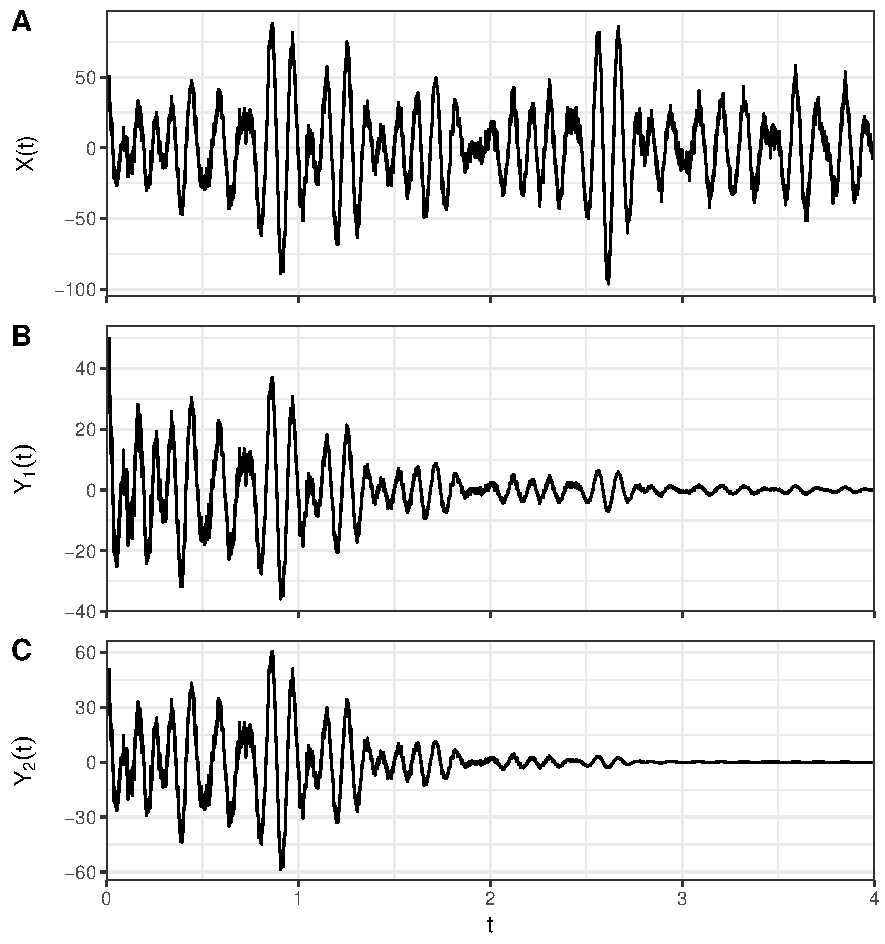
\includegraphics[width=\linewidth]{./img_mas_ejemplos/proceso_alfa_varios.pdf}
\caption[Proceso tipo alfa con algunas modificaciones]{Proceso tipo alfa, con algunas modificaciones descritas en los ejemplos \ref{ejemplo:lazy1} y \ref{ejemplo:lazy2}. \textbf{A.} Una realización del proceso tipo alfa, \xt. \textbf{B.} Una realización del proceso $Y_1(t) = X(t) e^{-\abso{t}}$. \textbf{C.} Una realización del proceso $Y_2(t) = e^{-\frac{t^2}{2}}$.}
\label{img:proceso_alfa_varios}
\end{figure}

\begin{ejemplo}
Sea \xtin{\R} un proceso tipo alfa, como se definió en el ejemplo \ref{lazy:proceso_alfa}. 
%
Ahora, se construye al proceso $\{Y_1(t)\}_{\R}$ como
\begin{equation}
Y_1(t) = X(t) e^{-\abso{t}}
\end{equation}
%
El núcleo de covarianza para $\{Y_1(t)\}_{\R}$ es
\begin{equation}
R_1(t,s) = \left[ \frac{\SEN{10 \pi (t-s)}}{(t-s)} - \frac{\SEN{7 \pi (t-s)}}{(t-s)} \right] e^{-\abso{t} } e^{-\abso{s}}
\end{equation}

Como se probó en el ejemplo \ref{ejemplo:oscilatorios1} las funciones $\phi(\omega; t) = e^{i \omega t} e^{-\abso{t}}$ son oscilatorias. $R_1$ admite una representación en términos de dichas funciones, ya que
\begin{align*}
R_1(t,s) &= R^\star(t-s) \left[e^{-\abso{t}}\right] \left[ e^{-\abso{s}} \right] \\
&= \left[e^{-\abso{t}}\right] \left[ e^{-\abso{s}} \right] \intR e^{i \omega (t-s)} dH_\star(\omega) \\
&= \intR \left[e^{-\abso{t}} e^{i \omega t} \right] \overline{\left[ e^{-\abso{s}} e^{i \omega s} \right]}  dH_\star(\omega)
\end{align*}
donde $H_\star$ es la función de espectro integrado para $X$. Entonces, el espectro evolutivo para $Y_1$, con respecto a la familia, es
\begin{equation}
dH_1(\omega;t) = e^{- 2 \abso{t}} dH_\star(\omega)
\end{equation}
%\begin{align*}
%\intR \overline{\left[ e^{i \omega s} e^{-\abso{s}} \right]} \left[ e^{i \omega t} e^{-\abso{t}} \right] dH(\omega) &= 
%\end{align*}
\label{ejemplo:lazy1}
\end{ejemplo}

\begin{ejemplo}
Sea \xtin{\R} un proceso tipo alfa, como se definió en el ejemplo \ref{lazy:proceso_alfa}. 
%
Ahora, se construye al proceso $\{Y_2(t)\}_{\R}$ como
\begin{equation}
Y_2(t) = X(t) e^{-\nicefrac{t^2}{2}}
\end{equation}
%
El núcleo de covarianza para $\{Y_2(t)\}_{\R}$ es
\begin{equation}
R_2(t,s) = \left[ \frac{\SEN{10 \pi (t-s)}}{(t-s)} - \frac{\SEN{7 \pi (t-s)}}{(t-s)} \right] e^{-\nicefrac{t^2}{2}} e^{-\nicefrac{s^2}{2}}
\end{equation}

De forma análoga al ejemplo anterior, el ejemplo \ref{ejemplo:oscilatorios2} se demostró que las funciones de la forma $\phi(\omega; t) = e^{i \omega t} e^{-\nicefrac{t^2}{2}}$ son oscilatorias. $R_2$ admite una representación en términos de dichas funciones como
\begin{equation}
R_2(t,s) = \left[e^{-\nicefrac{t^2}{2}} \right] \overline{\left[ e^{-\nicefrac{s^2}{2}} \right]}  dH_\star(\omega)
\end{equation}
donde $H_\star$ es la función de espectro integrado para $X$. Entonces, el espectro evolutivo para $Y_2$, con respecto a la familia, es
\begin{equation}
dH_2(\omega;t) = e^{-{t^2}} dH_\star(\omega)
\end{equation}
%\begin{align*}
%\intR \overline{\left[ e^{i \omega s} e^{-\abso{s}} \right]} \left[ e^{i \omega t} e^{-\abso{t}} \right] dH(\omega) &= 
%\end{align*}
\label{ejemplo:lazy2}
\end{ejemplo}

\begin{proposicion}
Sea \xt un proceso estocástico a tiempo continuo, débilmente estacionario, estocásticamente continuo, de media cero y varianza finita.
%
Entonces \xt es un proceso oscilatorio.
%
Más aún, la función de espectro integrado para \xt, $H_\star$, y su espectro evolutivo integrado con respecto a la familia $\{ e^{i \omega t} \}$, $H$, cumplen que
\begin{equation}
dH(\omega; t) = dH_\star(\omega)
\end{equation}
\label{lazy:redux}
\label{lazy11}
\end{proposicion}

\begin{proof}
Sea $R$ el núcleo de covarianza para \xt y sea $R^\star$ su función de autocorrelación. 
%$R^\star$ cumplen que
%es débilmente estacionario
%\begin{equation}
%R(s,t) = R^\star(\abso{t-s})
%\end{equation}
En virtud del teorema \ref{t_wienerkhinchin}, y porque el proceso es débilmente estacionario
%, se sabe que $R$ admite una representación de la forma
puede escribirse
\begin{equation}
R(s,t) = R^\star({t-s}) 
= \intR  \overline{\left[e^{i \omega {s}}\right]} \left[e^{i \omega {t}}\right]  dH_\star(\omega)
\end{equation}
%\begin{align*}
%R(s,t) &= R^\star({t-s}) \\
%&= \intR e^{i \omega (t-s)} dH(\omega) \\
%&= \intR  \overline{\left[e^{i \omega {s}}\right]} \left[e^{i \omega {t}}\right]  dH(\omega)
%\end{align*}
Previamente se mostró que las funciones de la forma $\phi(t) = e^{i \omega t}$ son oscilatorias, de donde se obtiene que \xt es un proceso oscilatorio.
%
De manera similar a los ejemplos anteriores, se deduce que el espectro evolutivo de \xt es
\begin{equation}
dH(\omega; t) = dH_\star(\omega)
\end{equation}
con lo cual se termina de demostrar la proposición.
\end{proof}

Antes de pasar al siguiente tema, conviene mostrar dos resultados que generalizan resultados presentados en capítulos anteriores: sobre la continuidad estocástica y sobre la representación espectral.

\begin{proposicion}
Sea \xt un proceso estocástico a tiempo continuo y $R$ su núcleo de covarianza.
%
Si $R$ es continuo en el conjunto $\left\{ (t,t) \in \R^2 \talque t\in \R \right\}$ entonces \xt es estocásticamente continuo.
\end{proposicion}

\begin{proposicion}
Sea \xt un proceso estocástico a tiempo continuo, estocásticamente continuo,  y sea $R$ su núcleo de covarianza.
%
Si $R$ admite una representación de la forma
\begin{equation}
R(s,t) = \intR \overline{\phi(\omega;s)}\phi(\omega;t) d\mu(\omega)
\end{equation}
entonces \xt acepta una representación de la forma
\begin{equation}
X(t) = \intR \phi(\omega; t) dZ(\omega)
\end{equation}
donde $\{ Z(t) \}_{t\in \R}$ es un proceso estocástico tal que
\begin{equation}
\Cov{Z(t),Z(s)} = \delta(t,z) \mu(\omega)
\end{equation}
con $\delta$ la función delta de Kronecker.
\end{proposicion}

La primera proposición se demuestra de forma similar a la proposición \ref{lazy:aaa}, aunque en este caso la implicación sólo es en una dirección.
%
La segunda proposición se demuestra de forma análoga al teorema \ref{rep_espectral}, reemplazando la participación del teorema de Wiener-Khintchine por el supuesto de que el núcleo de covarianza admite la representación descrita.

%%%%%%%%%%%%%%%%%%%%%%%%%%%%%%%%%%%%%%%%%%%%%%%%%%%%%%%%%%%%%%%%%%%%%%%%%%%%%%%%%%%%%%%%%%%%%%%%%%%
%%%%%%%%%%%%%%%%%%%%%%%%%%%%%%%%%%%%%%%%%%%%%%%%%%%%%%%%%%%%%%%%%%%%%%%%%%%%%%%%%%%%%%%%%%%%%%%%%%%

\section{Estimación del espectro evolutivo}
\label{sec:estimacion}

En el capítulo anterior --específicamente en la sección \ref{sec:estimadores}-- se exhibió un estimador consistente para la función de densidad espectral en procesos débilmente estacionarios, referido como \textit{estimador de ventana}.
% 
Dicho estimador se construye multiplicado al periodograma por una función con ciertas características, referida como \textit{ventana de retrasos}; se demostró que el estimador es insesgado para una \textit{versión suavizada} de la función de densidad espectral, siendo para ello un factor determinante la forma de la ventana de retrasos.
% \textit{suavizada} por un filtro lineal (también referido como función ventana).
%
En esta sección se exhibe una estimador similar para el espectro evolutivo; se presentan algunos teoremas sobre las propiedades de estos estimadores, así como algunas restricciones sobre los procesos para los cuales el estimador es \textit{útil}.
% exhiben algunos teoremas que permitan usar una técnica similar, la cual requiere imponer algunas condiciones más fuertes que ser oscilatorios.

\subsection{Filtros lineales sobre procesos oscilatorios}

Sea \xt un proceso oscilatorio, y sea $\mathcal{L}$ un filtro lineal cuya función de respuesta es $g\in \lldos$.
Se construye al proceso $\{Y(t)\}_{t\in \mathcal{T}}$ como\footnote{En el texto de Priestley se considera un filtro de la forma $Y(t) = \intR g(u) X(t-u) e^{-i \omega_0 (t-u)} du$ para algún $\omega_0$ constante. 
%
Por simplicidad se considera únicamente el caso $\omega_0=0$}
\begin{equation}
Y(t) = \intR g(u) X(t-u) du
\end{equation}

Entonces puede escribirse 
\begin{equation}
Y(t) = \intR \Gamma_t(\omega) e^{i \omega t} dZ(\omega) 
\label{se6:filtrado}
\end{equation}
donde $\Gamma_\bullet$ es la \textbf{función de transferencia generalizada} para $g$ con respecto a la familia $\ef$, y que es definida como
\begin{equation}
\Gamma_t (\omega) := \intR g(u) A(\omega; t-u) e^{i \omega u} du
\label{se6:trans_general}
\end{equation}

Conviene destacar el caso particular cuando $A$, como función de $\omega$, varía \textit{lentamente} en comparación de $g$; en tal caso podría decirse que $\Gamma_\bullet \approx \Gamma$ (un resultado similar al teorema \ref{lazy:rel_espectros}), con lo cual las consideraciones de la sección \ref{sec:estimadores} serían aproximadamente válidas incluso para procesos no-estacionarios.

\begin{definicion}
Una familia de funciones $\ef = \left\{ \phi: \R \times \mathcal{T} \rightarrow \C \right\}$ se dice \textbf{semi-estacionaria} si, para todo $t \in \mathcal{T}$, se cumple que
\begin{equation}
\intR \abso{\omega} \abso{dK_t(\omega)} < \infty
\end{equation}
donde $\phi(\omega; t) = \intR e^{i \omega t} dK_t(\omega)$. Si así fuere, se define el \textbf{ancho de banda característico} de $\ef$ como
\begin{equation}
B_\ef := \left[ \sup_\omega \intR \abso{\omega} \abso{dK(\omega)} \right]^{-1}
\end{equation}
\end{definicion}

\begin{ejemplo}
La familia de funciones $\{ \phi(t) = e^{i \omega t} \}$ es semi-estacionaria. Usando a $K$ como en el ejemplo \ref{ejemplo:sen_cos_oscilatorios}, se tiene que
\begin{equation}
\intR \abso{\omega} \abso{dK_t(\omega)} = 0
\end{equation}
El ancho de banda característico de la familia no está bien definido como un número real, pero si se usa a $\R\cup \{ \pm \infty \}$, su ancho de banda es $\infty$.
\label{lazy12}
\end{ejemplo}

\begin{ejemplo}
La familia de funciones $\{ \phi(t) = e^{i \omega t} e^{-\abso{t}} \}$ \textbf{no} es semi-estacionaria. Usando a $K_1$ como en el ejemplo \ref{ejemplo:oscilatorios1}, se tiene que
\begin{equation}
\intR \abso{\omega} \abso{dK_t(\omega)} = \frac{1}{\pi} \intR \frac{\omega}{1 + \omega^2} d\omega \nless \infty
\end{equation}
\end{ejemplo}

\begin{ejemplo}
La familia de funciones $\{ \phi(t) = e^{i \omega t} e^{-\nicefrac{t^2}{2}} \}$ es semi-estacionaria. Usando a $K_2$ como en el ejemplo \ref{ejemplo:oscilatorios2}, se tiene que
\begin{equation}
\intR \abso{\omega} \abso{dK_t(\omega)} = \intR e^{-\nicefrac{\omega^2}{2}} d\omega = \frac{1}{2}
\end{equation}
El ancho de banda característico para esta familia de funciones es 2.
\end{ejemplo}

\begin{definicion}
Un proceso \xt se dice \textbf{semi-estacionario} si su núcleo de covarianza, $R$, admite una representación de la forma 
\begin{equation}
R(s,t) = \intR \overline{\phi(\omega;s)}\phi(\omega;t) d\mu(\omega)
\label{lazy10}
\end{equation}
para alguna familia de funciones $\ef = \left\{ \phi: \R \times \mathcal{T} \rightarrow \C \right\}$ que es semi-estacionaria, y alguna función $\mu$.

Sea $\mathcal{C}_X$ la clase de las familias semi-estacionarias para las cuales el núcleo de covarianza de \xt admite una representación de la forma \ref{lazy10}. Se define a $B_X$, el \textbf{ancho de banda característico para} \xt, como
\begin{equation}
B_X := \sup_{\ef \in \mathcal{C}_X} B_\ef
\end{equation}
\label{def:semi_estacionario}
\end{definicion}

\begin{proposicion}
Sea \xt un proceso estocástico a tiempo continuo, débilmente estacionario, estocásticamente continuo, de media cero y varianza finita.
%
Entonces \xt es un proceso semi-estacionario, cuyo ancho de banda característico es $B_X = \infty$.
\end{proposicion}

\begin{proof}
En el ejemplo \ref{lazy11} se demostró que todos los procesos con las características descritas son oscilatorios, y que tienen asociada a la familia de funciones $\ef = \{ \phi(t) = e^{i \omega t} \}$.
%
En el ejemplo \ref{lazy12} se demostró que esa familia tiene un ancho de banda característico $B_\ef = \infty$.
%
Entonces es inmediato que el ancho de banda característico para \xt es $B_X=\infty$.
\end{proof}

%\begin{definicion}
%Sea \xt un proceso semi-estacioario, y sea $\mathcal{C}$ la clase de las familias semi-estacionarias con las cuales el proceso admite una representación de la forma [?].
%Se define el \textbf{ancho de banda característico} de \xt como 
%\begin{equation}
%B_X := \sup_{\ef \in \mathcal{C}} B_\ef
%\end{equation}
%\end{definicion}

\begin{definicion}
Sea $\mathcal{L}$ un filtro lineal, con $g$ su función de respuesta y $\Gamma$ su función de transferencia. Su \textbf{ancho de banda}, $B_g$, es
\begin{equation}
B_g := \intR \abso{u} \abso{g(u)} du
\end{equation}

Por simplicidad de referencia, en lo siguiente se dirá que $\mathcal{L}$ está normalizada si cumple que
%Supóngase que $g$ está normalizada de modo que
\begin{equation}
2 \pi \intR \abso{g(u)}^{2} du = \intR \abso{\Gamma(\omega)} d\omega = 1
\label{s6:norm_g}
\end{equation}
%con $\Gamma$ la función de respuesta para $g$.
\end{definicion}
%De manera similar, se define el \textbf{ancho de banda} para $g$ como 

\begin{definicion}
Se dice que una función $u : \R \rightarrow \C$ es \textbf{pseudo-$\boldsymbol{\delta}$ de orden $\boldsymbol{\varepsilon}$} con respecto a la función $v : \R \rightarrow \C$ si, para cualquier $k\in \R$ existe un $\varepsilon \ll 1$ tal que 
\begin{equation}
\abso{\intR u(x) v(x+k) dx  -  v(k)\intR u(x)} < \varepsilon
\end{equation}
\end{definicion}

\begin{teorema}
Sea $\ef$ una familia semi-estacionaria con ancho de banda característico $B_\ef$, y sea $g$ una función normalizada como en \ref{s6:norm_g} y cuyo ancho de banda es $B_g$. Entonces, para cualesquiera $t, \omega \in \R$ se cumple que $e^{i \omega t} dK(\omega)$ es una función pseudo-$\delta$ de orden $\nicefrac{B_g}{B_\ef}$ con respecto a $g$
\label{teo:s6:lema}
\end{teorema}
\begin{proof}
Suponiendo que $\Gamma$ sea una vez derivable, su expansión de Taylor alrededor de $k$ es
\begin{equation*}
\intR e^{i\theta t} \Gamma(\theta + k) dK(\omega)
= \Gamma(k) \intR e^{i \theta t} dK(\omega) + 
\intR e^{i \theta t} \theta \Gamma\prima(k + \nu) dK(\omega)
\end{equation*}
para algún $\nu \in (0,\theta)$. Respecto al segundo sumando, puede observarse que
\begin{align*}
\intR e^{i \theta t} \theta \Gamma\prima(k + \nu) dK(\omega)
&\leq
\abso{ \intR e^{i \theta t} \theta \Gamma\prima(k + \nu) dK(\omega)} \\
&\leq
\intR \abso{ \theta} \abso{ \Gamma\prima(k + \nu)} \abso{ dK(\omega)} \\
&\leq
\intR \abso{ \theta} \left[ \sup_\omega \abso{ \Gamma\prima(\omega)} \right] \abso{ dK(\omega)} \\
&\leq
\left[ \sup_\omega \abso{ \Gamma\prima(\omega)} \right]
\left[ \sup_\omega
\intR \abso{ \theta} \abso{ dK(\omega)} \right]
\end{align*}
Usando la conexión entre $g$ y $\Gamma$
\begin{align*}
\Gamma\prima(\omega) 
&= \frac{d}{d\omega} \left( \intR e^{i \omega u} g(u) du \right) \\
&= \intR \left( \frac{d}{d\omega} e^{i \omega u} g(u) \right) du \\
&= i \intR u e^{i \omega u} g(u) du \\
\end{align*}
Luego entonces
\begin{align*}
\intR e^{i \theta t} \theta \Gamma\prima(k + \nu) dK(\omega)
&\leq
\left[ \sup_\omega \abso{ \Gamma\prima(\omega)} \right] 
\left[ \sup_\omega
\intR \abso{ \theta} \abso{ dK(\omega)} \right] \\
&\leq 
\left[ \sup_\omega \abso{ \intR i u e^{i \omega u} g(u) du } \right] 
B_\ef^{-1} \\
&\leq 
B_\ef^{-1}
\left[ \sup_\omega \intR \abso{ u } \abso{ g(u)} du \right] \\
&\leq
B_\ef^{-1} B_g
\end{align*}
\end{proof}

Con el teorema anterior a la mano se puede declarar formalmente la idea de que $A$ varía más lentamente que $g$.

\begin{teorema}
Sea $\ef$ una familia semi-estacionaria con ancho de banda característico $B_\ef$, sea $\varepsilon >0$ arbitrario, y sea $g$ un filtro normalizado como en \ref{s6:norm_g} y cuya función de transferencia generalizada con respecto a $\ef$ es $\Gamma_\bullet$. 
%
Si $g$ es elegida de tal modo que $\nicefrac{B_g}{B_\ef} < \varepsilon$, entonces para cualesquiera $t, \omega$ se cumple que
\begin{equation}
\abso{\Gamma_t(\omega)- A(\omega; t)\Gamma(\omega)} < \varepsilon
\end{equation}
\label{teo:aprox_gamma} 
\end{teorema}

\begin{proof}
Por la mera definición de $\Gamma_\bullet$ (expresión \ref{se6:trans_general}) se sabe que
\begin{equation*}
\Gamma_t (\omega) = \intR g(u) A(\omega; t-u) e^{i \omega u} du
\end{equation*}
Si se sustituye a $A$ en términos de $dK$ (ver la definición de función oscilatoria)
\begin{align*}
\Gamma_t (\omega) &= \intR g(u) A(\omega; t-u) e^{i \omega u} du \\
&= 
\intR g(u) \left[ \intR e^{i \theta (t-u)} dK(\theta) \right] e^{i \omega u} du \\
&=
\intR \intR g(u) e^{i \theta t} e^{i (\omega- \theta) u} dK(\theta) du \\
&=
\intR e^{i \theta t} \left[ \intR g(u) e^{i (\omega- \theta) u} du \right] dK(\theta) \\
&=
\intR e^{i \theta t} \Gamma(\omega - \theta) dK(\theta) \\
\end{align*}
Usando el lema \ref{teo:s6:lema} junto al hecho que $\nicefrac{B_g}{B_\ef} < \varepsilon$, se puede escribir que
\begin{align*}
\varepsilon 
&> 
\abso{\intR e^{i \theta t} \Gamma(\omega - \theta) dK(\theta) - 
\Gamma(\omega) \intR e^{i \theta t} dK(\theta) } \\
&=
\abso{\Gamma_t (\omega) - 
\Gamma(\omega) \intR e^{i \theta t} dK(\theta) } \\
&=
\abso{\Gamma_t (\omega) - 
\Gamma(\omega) A(\omega; t) }
\end{align*}
En el último renglón se ha reemplazado nuevamente a $A$ en términos de $dK	$
\end{proof}

\begin{teorema}
Sea \xt un proceso semi-estacionario con ancho de banda característico $B_X$, sea $g$ un filtro normalizado como en \ref{s6:norm_g} y cuyo ancho de banda es $B_g$ y cuya función de respuesta es $\Gamma$. 
%
Sea $\{Y(t)\}_{t\in \mathcal{T}}$ un proceso definido como \ref{se6:filtrado}.
%
Sea $\efstar$ una familia semi-estacionaria cuyo ancho de banda característico es $B_X$ o es muy parecido a $B_X$ (lo cual es posible por cómo se definió $B_X$).
%
Se cumple que
\begin{equation}
\E{\abso{Y(t)}^{2}} = \intR \abso{\Gamma(\omega)}^{2} dH^{*}(\omega; t) + \orden{\varepsilon}
\end{equation}
donde $H^{*}$ es el espectro integrado respecto a la familia $\efstar$ y $\orden{\varepsilon}$ es un término que puede hacerse arbitrariamente pequeño si $B_g$ es pequeño respecto a $B_X$.
\label{teo:aprox_orden}
\end{teorema}

\begin{proof}
Usando la expresión \ref{se6:filtrado} para este caso particular, puede escribirse
\begin{equation}
Y(t) = \intR \Gamma_t^{*} (\omega; t) A^{*}(\omega; t) e^{i \omega t} dZ^{*}(\omega)
\end{equation}
donde $\omega_\bullet^{*}$, $A^{*}$ y $Z^{*}$ están definidos respecto a la familia $\efstar$.
Nótese que, debido a que los $dZ$'s son ortogonales
%\begin{align*}
%\E{\abso{Y(t)}^{2}} 
%&= 
%\E{
%\overline{\intR \Gamma_t^{*} (\omega; t) e^{i \omega t} dZ^{*}(\omega)}
%\intR \Gamma_t^{*} (\omega; t) e^{i \omega t} dZ^{*}(\omega) }\\
%&= ... \\
%&= \intR \abso{\Gamma_t^{*} (\omega; t)}^{2} d\mu^{*}(\omega)
%\end{align*}
\begin{align*}
\E{\abso{Y(t)}^{2}} 
&= \intR \abso{\Gamma_t^{*} (\omega; t)}^{2} d\mu^{*}(\omega)
\end{align*}

Si se elige a $g$ de modo que $\frac{B_g}{B_X} < \varepsilon$, en virtud del teorema \ref{teo:aprox_gamma} puede escribirse
\begin{equation}
\Gamma_t^{*}(\omega; t) = A^{*}(\omega; t) \Gamma(\omega) + R(\omega; t)
\end{equation}
con $\abso{R(\omega,t)} < \varepsilon$. Luego entonces
\begin{align*}
\E{\abso{Y(t)}^{2}} 
&= 
\intR \abso{\Gamma_t^{*} (\omega; t)}^{2} d\mu^{*}(\omega) \\
&= 
\intR \abso{A^{*}(\omega; t) \Gamma(\omega) + R(\omega; t)}^{2} d\mu^{*}(\omega) \\
&= 
\intR \abso{A^{*}(\omega; t) \Gamma(\omega)}^{2} d\mu^{*}(\omega) +\\
&\pheq
\intR \overline{A^{*}(\omega; t) \Gamma(\omega)} R(\omega; t) d\mu^{*}(\omega) +\\
&\pheq
\intR A^{*}(\omega; t) \Gamma(\omega) \overline{ R(\omega; t)} d\mu^{*}(\omega) +\\
&\pheq
\intR \abso{R(\omega; t)}^{2} d\mu^{*}(\omega) 
\end{align*}

El cuarto sumando satisface claramente que
\begin{equation}
\intR \abso{R(\omega; t)}^{2} d\mu^{*}(\omega)  < \varepsilon^{2} \intR d\mu^{*}(\omega) 
= \orden{\varepsilon^{2}}
\end{equation}

Respecto al segundo sumando, nótese que 
\begin{align*}
\intR \overline{A^{*}(\omega; t) \Gamma(\omega)} R(\omega; t) d\mu^{*}(\omega)
&< \intR \abso{A^{*}(\omega; t)} \abso{ \Gamma(\omega)} \abso{R(\omega; t)} d\mu^{*}(\omega) \\
&< \varepsilon \intR \abso{A^{*}(\omega; t)}\abso{ \Gamma(\omega)} d\mu^{*}(\omega)
\end{align*}
Una cota similar puede hallarse para el tercer sumando.
Falta demostrar que la cota permanece finita cuando $B_g \rightarrow 0$, lo cual debería lograrse definiendo el conjunto
\begin{equation}
\Omega = \left\{ \omega \in \R \talque \abso{\Gamma(\omega)} \abso{A^{*}(\omega; t)} \leq 1 \right\} 
\end{equation}
y luego, claramente
\begin{equation}
\intR \abso{A^{*}(\omega; t)}\abso{ \Gamma(\omega)} d\mu^{*}(\omega) = 
\int_\Omega \mu^{*}(\omega) + 
\int_{\Omega^{C}} \abso{A^{*}(\omega; t)}\abso{ \Gamma(\omega)} d\mu^{*}(\omega)
\end{equation}
el primer sumando es claramente finito y no depende de $g$, mientras que el segundo debería ser finito ya que $\Gamma$ está normalizada.
\end{proof}

%\begin{proposicion}
%Si un proceso \xt es débilmente estacionario, entonces su espectro de potencias $h$ y su espectro evolutivo $h^{\star}$ satisfacen, para todo $t\in \mathcal{T}$, que
%\begin{equation}
%h^{\star}(\omega, t) = h(\omega)
%\end{equation}
%
%\end{proposicion}

%%%%%%%%%%%%%%%%%%%%%%%%%%%%%%%%%%%%%%%%%%%%%%%%%%%%%%%%%%%%%%%%%%%%%%%%%%%%%%%%%%%%%%%%%%%%%%%%%%%
%%%%%%%%%%%%%%%%%%%%%%%%%%%%%%%%%%%%%%%%%%%%%%%%%%%%%%%%%%%%%%%%%%%%%%%%%%%%%%%%%%%%%%%%%%%%%%%%%%%

\section{Estimador de doble ventana}
\label{sec:doble_ventana}

Para esta sección se considera un proceso a tiempo continuo \xtin{\R} y una muestra del mismo de longitud $T$ (o equivalentemente un proceso \xtin{[0,T]}), suficientemente larga. El objetivo en esta sección es construir un estimador para el espectro evolutivo $dH(\omega; t)$.
%
Por simplicidad, se supondrá que la medida $\mu$ es absolutamente continua respecto a la medida de Lebesgue, y entonces puede escribirse
\begin{equation}
h(\omega,t) := dH(\omega; t)
\end{equation}

Para efectuar la estimación del espectro se hará uso del teorema \ref{teo:aprox_gamma}, para lo cual se necesita un filtro $g$ normalizado según \ref{s6:norm_g} y cuyo ancho de banda, $B_g$, satisface
\begin{equation}
B_g \ll B_X \ll T
\label{s6:anchos_banda}
\end{equation}

Bajo estas condiciones se construye $U$ aplicando a $X$ un filtro lineal cuya función de respuesta es $g$
%Se construye entonces a $U$, una versión filtrada de $X$ usando a $g$
\begin{equation}
U(t) = \int_{t-T}^{t} g(u) X(t-u) du
\end{equation}

Bajo la condición \ref{s6:anchos_banda}, la integral que define a $U$ puede extenderse a todo $\R$ sin cambiar mucho su valor (excepto cerca de 0 y $T$), e incluso se llega a ser exacta si $g$ es 0 fuera de un intervalo pequeño alrededor de 0. Entonces, en virtud del teorema \ref{teo:aprox_orden}
aplica de manera aproximada, y entonces se cumple que
\begin{equation}
\E{\abso{U(\omega; t)}^{2}} = \intR \abso{\Gamma(\omega)}^{2} h(\omega, t)d\omega + \orden{\nicefrac{B_g}{B_X}}
\end{equation}


El teorema de Isserlis es una identidad relativamente poco conocida sobre los cuartos momentos de una distribución multinormal; el caso particular de cuatro variables será usado para calcular la covarianza de algunos estimadores del espectro de potencias.

\begin{teorema}[Isserlis]
Sea $[X_1, X_2, X_3, X_4]$ un vector aleatorio siguiendo una distribución multinormal con media cero y matriz de covarianza finita. Se cumple que
\begin{equation}
\E{X_1 X_2 X_3 X_4} = \E{X_1 X_2} \E{X_3 X_4} + \E{X_1 X_3} \E{X_2 X_4} + \E{X_1 X_4} \E{X_2 X_3}
\end{equation}
\label{teo:isserlis}
\end{teorema}

%\begin{proof}
%Si $\phi$ es la función característica de $(X_1, X_2, X_3, X_4)$, entonces puede escribirse
%\begin{equation}
%\E{X_1 X_2 X_3 X_4} = \frac{\partial^{2}}{\partial s_1 \partial s_2 \partial s_3 \partial s_4} \phi(s_1, s_2, s_3, s_4) \vert_{s_i = 0}
%\end{equation}
%
%[?] completar, no es dificil
%\end{proof}

\begin{proposicion}
Dadas las condiciones, y si \xt es un proceso normal que admite un espectro evolutivo uniformemente continuo, se tiene que
\begin{equation}
\Var{\abso{U(\omega;t)}^{2}} = \left[ \intR \abso{\Gamma(\omega)}^{2} h(\omega, t)d\omega \right]^{2} + \orden{\nicefrac{B_g}{B_X}}
\end{equation}
\end{proposicion}

%La demostración al teorema anterior puede ahllarse en el artículo de Maurice Priestley \textit{Design Relations for Non-Stationary Processes} \cite{Priestley66}, sección 3.

\begin{proof}
Por conveniencia se obtendrá una expresión aproximada para la covarianza de $U$, a partir de la cual se deducirá su varianza. 
%
Para ello, por definición puede escribirse para $t,s \in \mathcal{T}$ y $\omega, \lambda \in \R$
\begin{align*}
\Cov{\abso{U(\omega;t)}^{2},\abso{U(\lambda;s)}^{2}} =
\E{\abso{U(\omega;t)}^{2} \abso{U(\lambda;s)}^{2}} - 
\E{\abso{U(\omega;t)}^{2}} \E{\abso{U(\lambda;s)}^{2}}
\end{align*}
\begin{multline}
\E{\abso{U(\omega;t)}^{2} \abso{U(\lambda;s)}^{2}}
=
\iiiint_{\R^{4}} g(u) g(v) g(w) g(z) e^{i u \omega} e^{i v \omega} e^{i w \lambda} e^{i z \lambda} \\
 \times
\E{{X(t-u)} {X(t-v)} {X(s-w)} {X(s-z)}}
du dv dw dz 
\end{multline}
Si para cada $t$ $X(t)$ sigue una distribución normal, entonces en virtud del teorema \ref{teo:isserlis} puede escribirse
\begin{align*}
\E{X(t-u) {X(t-v)} {X(t-w)} X(t-z)} 
&=       R(t-u,t-v)R(s-w,s-z) \\
&\pheq + R(t-u,s-z)R(t-v,s-w) \\
&\pheq + R(t-u,s-w)R(t-v,s-z)
\end{align*}
Reemplazando sobre la expresión anterior, puede escribirse
\begin{equation}
\E{\abso{U(\omega;t)}^{2} \abso{U(\lambda;s)}^{2}} = \E{\abso{U(\omega;t)}^{2}} \E{\abso{U(\lambda;s)}^{2}}+ S_1 + S_2
\end{equation}
donde
\begin{multline*}
S_1 = \iiiint_{\R^{4}} g(u) g(v) g(w) g(z) e^{i u \omega} e^{i v \omega} e^{i w \lambda} e^{i z \lambda} \\
\times
R(t-u,s-z)R(t-v,s-w)
du dv dw dz 
\end{multline*}
Se define a $S_2$ de manera similar, intercambiando $w$ y $z$. 
%
Estas expresiones, de apariencia innecesariamente complicada, pueden interpretarse como las \textit{interferencias} de la covarianza entre los puntos $(\omega, t)$ y $(\lambda,s)$.
%
Para ello, nótese que
\begin{equation}
\Cov{\abso{U(\omega;t)}^{2},\abso{U(\lambda;s)}^{2}} = S_1 + S_2 + \orden{\nicefrac{B_g}{B_X}}
\end{equation}
%
Cabe mencionar que es conveniente que las cantidades $S_1$ y $S_2$ sean pequeñas.

Sea ha elegido a $g$ de forma que $B_g \ll B_X$ con el objetivo de que $U$ tenga un sesgo pequeño, en virtud del teorema \ref{teo:aprox_orden}. Este teorema puede ser usado nuevamente si $S_1$ y $S_2$ son reescritas en cierta forma \textit{adecuada}, para lo cual la autocovarianza debe ser vista como
\begin{equation}
R(p,q) = \intR e^{i \omega (p-q)} A(\omega; p)\overline{A(\omega; q)} d\mu(\omega) 
\end{equation}
Así pues, reemplazando esta expresión sobre (?) se obtiene
\begin{align*}
S_1 &=
\iiiint_{\R^{4}} g(u) g(v) g(w) g(z) e^{i u \omega} e^{i v \omega} e^{i w \lambda} e^{i z \lambda} \\
&\pheq \times R(t-u,s-z)R(t-v,s-w) du dv dw dz \\
&= 
\iiiint_{\R^{4}} g(u) g(v) g(w) g(z) e^{i u \omega} e^{i v \omega} e^{i w \lambda} e^{i z \lambda} \\
&\pheq \times \left( 
\iint_{\R^{2}} 
\left[ 
e^{-i \theta (s-z-t+u)} A(\theta; t-u) \overline{A(\theta; s-z)} 
\right] 
\right. \\
&\pheq 
\left. \vphantom{\int} \phantom{times}
\left[ e^{-i \phi (s-w-t+u)} A(\phi; t-v) \overline{A(\theta; s-w)} \right] d\theta d\phi
\right) du dv dw dz
\\
 &= \iint_{\R^{2}} \Gamma_*(\theta+ \omega; t, \theta) \overline{\Gamma_*(\phi + \omega; t, \phi)}
 \Gamma_*(\phi+ \lambda; s, \phi) \overline{\Gamma_*(\theta + \lambda; s, \theta)} \\
 &\pheq \times
 \left[
 A(\theta; t) \overline{A(\phi; t)} A(\phi; s) \overline{A(\theta; t)}
 \right] d\theta d\phi
\\
 &= \left[ \intR \overline{\Gamma_*(\phi + \omega; t, \phi)} \Gamma_*(\phi+ \lambda; s, \phi)
 \overline{A(\phi; t)} A(\phi; s) d\phi \right] \\
 &\pheq \times \left[ \int_{\R^{2}} \Gamma_*(\theta+ \omega; t, \theta) 
  \overline{\Gamma_*(\theta + \lambda; s, \theta)}  
 A(\theta; t)   \overline{A(\theta; t)} d\theta \right] 
\end{align*}
Donde $\Gamma_*$ es la función de transferencia generalizada
\begin{equation}
\Gamma_*(\kappa; t, \omega) = \intR g(u) \frac{A(\omega; t-u)}{A(\omega; t)} e^{-i u \kappa} du
\end{equation}
Usando el teorema \ref{teo:aprox_gamma}, se puede decir que $\abso{\Gamma(\bullet; t, \lambda) - \Gamma(\bullet)} \leq \nicefrac{B_g}{B_X}$. Así entonces
\begin{align*}
\abso{S_1} &=
 \abso{ \intR \overline{\Gamma_*(\phi + \omega; t, \phi)} \Gamma_*(\phi+ \lambda; s, \phi)
 \overline{A(\phi; t)} A(\phi; s) d\phi } \\
 &\pheq \times \abso{ \int_{\R^{2}} \Gamma_*(\theta+ \omega; t, \theta) 
  \overline{\Gamma_*(\theta + \lambda; s, \theta)}  
 A(\theta; t)   \overline{A(\theta; t)} d\theta } \\ 
 &\leq
 \left[ \intR \abso{\Gamma_*(\phi + \omega; t, \phi)} \abso{\Gamma_*(\phi+ \lambda; s, \phi)}
 \abso{A(\phi; t) A(\phi; s)} d\phi \right] \\
 &\pheq \times \left[ \int_{\R^{2}} \abso{\Gamma_*(\theta+ \omega; t, \theta)} 
  \abso{\Gamma_*(\theta + \lambda; s, \theta)}  
 \abso{A(\theta; t) A(\theta; t)} d\theta \right] \\ 
 &\leq
 \left[ \intR \abso{\Gamma(\phi + \omega)} \abso{\Gamma(\phi+ \lambda)}
 \abso{A(\phi; t) A(\phi; s)} d\phi \right]^{2} + \orden{\nicefrac{B_g}{B_X}}
\end{align*}
La misma cota puede hallarse para $S_2$. En lo inmediato, conviene analizar el caso $\omega = \lambda$ y $t = s$, de donde se obtiene
\begin{align*}
\Var{\abso{U(\omega; t)}^{2}} &= \Cov{\abso{U(\omega; t)}^{2}, \abso{U(\omega; t)}^{2}} = S_1 + S_2 + \orden{\nicefrac{B_g}{B_X}}
\end{align*}
pero en este caso particular, la cota obtenida puede reducirse a
\begin{align*}
\abso{S_1} & \leq
\left[ \intR \abso{\Gamma(\phi + \omega)}^{2} \abso{A(\phi; t)}^{2} d\phi \right]^{2} + \orden{\nicefrac{B_g}{B_X}} \\
&= 
\left[ \intR \abso{\Gamma(\phi + \omega)}^{2} h(\phi, t) d\phi \right]^{2} + \orden{\nicefrac{B_g}{B_X}}
\end{align*}
\end{proof}

En el teorema anterior puede interpretarse que $\intR \abso{\Gamma(\phi + \omega)}^{2} h(\phi, t) d\phi$ es una versión \textit{suavizada} de $h$.
%
Bajo este comentario, el resultado obtenido es muy análogo a la estimación del espectro en un proceso estacionario (teorema \ref{lazy-algo}).
%
Siguiendo dicha analogía, se sabe que $U$ puede \textit{modificarse} para generar estimadores consistentes; para lo cual se usa una segunda función de ventana $w_\tau$. 
%
Por estética y comodidad, las condiciones sobre $w_\tau$ serán presentadas junto a las propiedades de la ventana $g$; todas ellas en la definición

\begin{definicion}
El \textbf{estimador de doble ventana} es un estimador para $h$ definido como
\begin{equation}
\widehat{h}(\omega, t) = \int_{T-t}^{t} w_\tau (u) \abso{U(\omega,t-u)}^{2} du
\end{equation}
donde la función $g$ satisface
\begin{itemize}
\item $B_g \ll B_X \ll T$
\item $g(t) \rightarrow 0$ cuando $\abso{t} \rightarrow \infty$
\item $2\pi \intR \abso{g(u)}^{2} du = \intR \abso{\Gamma(\omega)}^{2} d\omega = 1$
\end{itemize}
con $\Gamma(\lambda) = \intR e^{-i \lambda t} g(t) d\lambda$. Así mismo, la función $w_\tau$ satisface
\begin{itemize}
\item $w_\tau(t) \geq 0$ para cualesquiera $t$, $\tau$
\item $w_\tau(t) \rightarrow 0$ cuando $\abso{t} \rightarrow \infty$, para todo $\tau$
\item $\displaystyle \intR w_\tau(t) dt = 1$ para todo $\tau$
\item $\displaystyle \intR \left( w_\tau(t) \right)^{2} dt < \infty$ para todo $\tau$
\item $\exists C \in \R$ tal que  
$\displaystyle \lim_{\tau\rightarrow\infty} \tau \intR \abso{ W_{\tau}(\lambda) }^{2} d\lambda = C$
\end{itemize}
donde $W_\tau(\lambda) = \intR e^{-i \lambda t} w_\tau(t) d\lambda$.
\label{estimador_doble_ventana}
\end{definicion}

El supuesto sobre que $w_\tau$ decaiga rápidamente lejos de 0 permite reemplazar el intervalo de integración que define a $\widehat{h}$ por $\R$ (excepto cerca de 0). 

\begin{proposicion}
El estimador de doble ventana satisface
\begin{equation}
\E{\widehat{h}(\omega, t)} = \intR \abso{\Gamma(\omega)}^{2} \overline{h}(\omega,t) d\omega du +
\orden{\nicefrac{B_g}{B_X}}
\end{equation}
donde
\begin{equation}
\overline{h}(\omega,t) = \intR w_\tau (u) h(\omega, t-u) du
\end{equation}
\label{lazy:med_dd}
\end{proposicion}

\begin{proof}
De manera relativamente sencilla puede verificarse que
\begin{align*}
\E{\widehat{h}(\omega,t)} &= 
\E{\intR w_\tau (u) \abso{U(t-u)}^{2} du} \\
&= 
\int_{T-t}^{t} w_\tau (u) \E{\abso{U(t-u)}^{2}} du \\
&=
\intR w_\tau (u) \left[
\intR \abso{\Gamma(\omega)}^{2} h(\omega, t-u)d\omega + \orden{\nicefrac{B_g}{B_X}} \right] du \\
&=
\intR \intR w_\tau (u) \abso{\Gamma(\omega)}^{2} h(\omega, t-u)d\omega du +
\orden{\nicefrac{B_g}{B_X}} \intR w_\tau (u) du \\
&=
\intR \abso{\Gamma(\omega)}^{2} \left[ \intR w_\tau (u) h(\omega, t-u) du \right] d\omega du +
\orden{\nicefrac{B_g}{B_X}} \\
&=
\intR \abso{\Gamma(\omega)}^{2} \overline{h}(\omega,t) d\omega du +
\orden{\nicefrac{B_g}{B_X}}
\end{align*}
\end{proof}

A diferencia de $U$, el estimador de doble ventana no es consistente salvo en caso que $\overline{h}$ sea parecido a $h$; como $\overline{h}$ es una versión suavizada, que el estimador sea sesgado depende de que $B_{w_\tau}$ sea pequeño en comparación a $B_X$.

\begin{proposicion}
El estimador de doble ventana satisface
\begin{equation}
\Var{V(t)} \approx \widetilde{h}^{2}(\omega_0,t) \left[ \intR \abso{W_\tau(\omega)}^{2} d\omega \right] \left[ \intR \abso{\Gamma(\omega)}^{4} \right] (1+\delta(0,\omega_0))
\end{equation}
donde
\begin{equation}
\widetilde{h}^{2} = \frac{\intR h^{2}(\omega_0,t) \left(w_\tau(u)\right)^{2}}{\intR \left(w_\tau(u)\right) du}
\end{equation}
\label{lazy:var_estdd}
\end{proposicion}

\begin{proof}
Como en el caso del estimador $U$, será conveniente calcular la covarianza de $\widehat{h}$ y posteriormente deducir la varianza. Se escribe para $t, s \in \mathcal{T}$ y $\omega, \lambda \in \R$
\begin{equation}
\Cov{\widehat{h}(\omega, t),\widehat{h}(\lambda, s)} = \E{\widehat{h}(\omega, t)\widehat{h}(\lambda, s)} - \E{\widehat{h}(\omega, t)}\E{\widehat{h}(\lambda, s)}
\end{equation}
Hecho el trabajo previo, es claro que
\begin{align*}
\Cov{\widehat{h}(\omega, t), \widehat{h}(\lambda, s)} &=
\iint_{\R^{2}} w_\tau(u) w_\tau(v) \Cov{\abso{U(\omega; t-u)}^{2},\abso{U(\lambda; s-v)}^{2}} du dv \\
&=
\iint_{\R^{2}} w_\tau(u) w_\tau(v) \left[ S_1 + S_2 \right] du dv + \orden{\nicefrac{B_g}{B_X}} \\
&= T_1 + T_2
\end{align*}
usando, por comodidad
\begin{equation}
T_1 = \iint_{\R^{2}} w_\tau(u) w_\tau(v) \left[ S_1 \right] du dv
\end{equation}
y similarmente para $T_2$; $S_1$ es como en la expresión (?), evaluado en los puntos $(t-u,\omega), (s-v, \lambda)$
\begin{align*}
S_1 &=
 \left[ \intR \overline{\Gamma_*(\phi + \omega; t-u, \phi)} \Gamma_*(\phi+ \lambda; s-v, \phi)
 \overline{A(\phi; t-u)} A(\phi; s-v) d\phi \right] \\
 &\pheq \times \left[ \intR \Gamma_*(\theta+ \omega; t-u, \theta) 
  \overline{\Gamma_*(\theta + \lambda; s-v, \theta)}  
 A(\theta; t-u)   \overline{A(\theta; s-v)} d\theta \right] 
\end{align*}
con $\Gamma_*$ es la función de transferencia generalizada; $S_2$ se define de manera similar.
Se usará el teorema * para acotar la covarianza, comenzando por el primer sumando
\begin{align*}
T_1 &= 
\iint_{\R^{2}} w_\tau(u) w_\tau(v) \left[ S_1 \right] du dv \\
&\leq
\iint_{\R^{2}} w_\tau(u) w_\tau(v) \abso{ S_1 } du dv \\
&\leq 
\iint_{\R^{2}} 
w_\tau(u) w_\tau(v) \\
&\pheq 
 \times \left[ \intR
 \abso{\Gamma(\phi + \omega)} \abso{\Gamma(\phi+ \lambda)}
 \abso{A(\phi; t-u) A(\phi; s-v)} d\phi \right]^{2}
 du dv + \orden{\nicefrac{B_g}{B_X}} \\
&\leq 
\iint_{\R^{2}} \abso{\Gamma(\phi + \omega)} \abso{\Gamma(\phi+ \lambda)}
\abso{\Gamma(\theta + \omega)} \abso{\Gamma(\theta+ \lambda)} \\
&\pheq 
 \times \left[ \iint_{\R^{2}}  w_\tau(u) w_\tau(v)
 \abso{A(\phi; t-u) A(\phi; s-v)} du dv \right]
 d\phi d\theta + \orden{\nicefrac{B_g}{B_X}} \\
\end{align*}
\end{proof}


Aún más, si se usa la propiedad en el límite de $\tau W_\tau$ se puede escribir
\begin{equation}
\Var{V(t)} \approx 
\widetilde{h}^{2}(\omega_0,t) \frac{C}{\tau} \left[ \intR \abso{\Gamma(\omega)}^{4} \right] (1+\delta(0,\omega_0))
\end{equation}

Una aproximación muy similar 
puede hacerse respecto al segundo término, de modo que $\widetilde{h}\approx h$ y 
$\overline{h}^{2}\approx h^{2}$.
Tales aproximaciones serán mejores en tanto las ventanas $w_{\tau}$ y $W_{\tau}$ sean más 
cercanas a funciones tipo \dirac.
Dicho esto, se pueden hacer las siguientes aproximaciones, un poco más arriesgadas:
\begin{itemize}
\item $\displaystyle \E{\est{h}(t,\omega)} \approx h(t,\omega)$
\item $\displaystyle \Var{\est{h}(t,\omega)} \approx 
\frac{C}{\tau} h^{2}(t,\omega) \intR \abso{\Gamma_\kappa (\theta)}^{4} d\theta$
\end{itemize}

%%%%%%%%%%%%%%%%%%%%%%%%%%%%%%%%%%%%%%%%%%%%%%%%%%%%%%%%%%%%%%%%%%%%%%%%%%%%%%%%%%%%%%%%%%%%%%%%%%%
%%%%%%%%%%%%%%%%%%%%%%%%%%%%%%%%%%%%%%%%%%%%%%%%%%%%%%%%%%%%%%%%%%%%%%%%%%%%%%%%%%%%%%%%%%%%%%%%%%%

\section{Prueba de Priestley-Subba Rao}
\label{sec:psr}

La prueba de estacionariedad usada en el presente trabajo, fue propuesta por Priestley y Subba Rao en la década de 1960 \cite{Priestley69}.
%
Dicha prueba consiste en probar estadísticamente si el espectro evolutivo de un proceso dado puede reducirse a un espectro de potencias, como en el teorema \ref{lazy:redux}, lo cual es equivalente a probar si el proceso es débilmente estacionario.
%; en otras palabras, se prueba la hipótesis de que el espectro evolutivo efectivamente cambia en el tiempo. 
%
%Naturalmente, la prueba debe construirse sobre una única realización del proceso.
%
El procedimiento consiste en los siguientes pasos:
\begin{enumerate}
\item Estimar el espectro evolutivo en algunos puntos en tiempo y frecuencia.
\item Calcular el logaritmo para \textit{estabilizar} al estimador.
\item Efectuar una ANOVA de dos vías para verificar si el espectro cambia en el tiempo.
\end{enumerate}

%El procedimiento consiste en estimar el espectro evolutivo del proceso para algunos tiempos y frecuencias, usando en particular el estimador de doble ventana; dichos puntos deben ser tales que los estimadores sean aproximadamente no-correlacionados.
%%
%Posteriormente se calcula el logaritmo de la estimación obtenida con el fin de \textit{estabilizar} la varianza.
%%
%Finalmente, como parte central, se efectúa un ANOVA de dos vías para verificar si se puede afirmar que el espectro estimado tiene --estadísticamente-- el mismo valor en los diferentes puntos a través del tiempo.
%%
%Cabe destacar que este último paso tiene una interpretación poco convencional, y es que los estimadores tienen (por diseño) ciertas propiedades

El primer paso, está sujeto a todas las restricciones descritas anteriormente en el presente capítulo.
%
Por notación, sea \xtd un proceso semi-estacionario a tiempo discreto, de media cero y varianza finita cuya frecuencia de muestreo es $\Delta_t=1$; y sea \xtd un conjunto de $N$ observaciones.
%
Usando esta información se calcula para estos datos el estimador de doble ventana, $\widehat{h}$; para ello se eligen las funciones ventana $g_\kappa$ y $w_\tau$ que, por simplicidad, son ventanas de escalamiento con parámetros $\kappa$ y $\tau$. 
%
Sus funciones de transferencia serán $\Gamma_\kappa$ y $W_\tau$, respectivamente.

\begin{proposicion}
Sea $g$ una función cuando menos dos veces derivable cuyo dominio es $\mathcal{D}_g$, y sea $X$ una variable aleatoria real tal que $P(X\notin \mathcal{D}) = 0$. 
%
Pueden usarse las siguientes aproximaciones
\begin{align}
\E{g(X)} &\approx g\left( \E{X} \right) \\
\Var{g(X)} &\approx \Var{X} \left[ g\prima \left( \E{X} \right) \right]^{2}
\end{align}
\end{proposicion}

\begin{proof}
Se construye para $g$ su polinomio de Taylor de grado 2
%Usando polinomio de Taylor de grado 2 para $g$, 
alrededor de $\E{X}$, y éste es evaluado en $X$
\begin{equation}
g(X) = g\left( \E{X} \right) + \left(X - \E{X} \right) g\prima \left( \E{X} \right) + \frac{\left( X - \E{X} \right)^{2}}{2} g^{\prime \prime}(\xi)
\label{detalle:aprox}
\end{equation}
donde la variable aleatoria $\xi$ satisface $\abso{X-\xi} \leq \abso{X - \E{X}}$.
%
La aproximación, con una obvia pérdida, consiste en considerar que $\frac{1}{2}\left( X - \E{X} \right)^{2} g^{\prime \prime}(\xi) \approx 0$.
\begin{equation}
g(X) \approx g\left( \E{X} \right) + \left(X - \E{X} \right) g\prima \left( \E{X} \right)
\end{equation}
Si se toma el valor esperado de ambos lados
\begin{align}
\E{g(X)} &\approx \E{g\left( \E{X} \right)} + \E{\left(X - \E{X} \right)} g\prima \left( \E{X} \right) = g\left( \E{X} \right)
\end{align}

Lo cual confirma la primera parte del resultado. Para verificar la segunda parte del mismo, se elevan ambos lados al cuadrado
\begin{align}
\left[g(X)\right]^{2} &\approx \left[g\left( \E{X} \right)\right]^{2} + 2 g\left( \E{X} \right) \left(X - \E{X} \right) g\prima \left( \E{X} \right) \nonumber \\
&\pheq + \left(X - \E{X} \right)^{2} \left[ g\prima \left( \E{X} \right] \right)^{2}
\end{align}

Posteriormente se toma el valor esperado de ambos lados
\begin{align*}
\E{\left[g(X)\right]^{2}} &\approx \E{\left[g\left( \E{X} \right)\right]^{2}} + 2 g\left( \E{X} \right) \E{X - \E{X} } g\prima \left( \E{X} \right) \nonumber \\
&\pheq + \E{\left(X - \E{X} \right)^{2}} \left[ g\prima \left( \E{X} \right] \right)^{2} \\
&= \left[g\left( \E{X} \right)\right]^{2} + \Var{X} \left[ g\prima \left( \E{X} \right] \right)^{2}
\end{align*}
entonces
\begin{equation}
\Var{g(X)} = \E{\left[g(X)\right]^{2}} - \left[g\left( \E{X} \right)\right]^{2} \approx \Var{X} \left[ g\prima \left( \E{X} \right] \right)^{2}
\end{equation}
de donde se obtiene la segunda parte del resultado. 

%Antes de concluir la demostración, conviene discutir bajo qué condiciones la aproximación es eficiente. La forma completa de la expresión \ref{detalle:aprox} contempla el término
%\begin{equation}
%\frac{\left( X - \E{X} \right)^{2}}{2} g^{\prime \prime}(\xi)
%\end{equation}
%Como $\abso{\xi} < $
\end{proof}

\begin{corolario}
Si se usa el teorema anterior con $g = \log$ se obtiene
\begin{align}
\E{\log(X)} &\approx \log\left( \E{X} \right) \\
\Var{\log(X)} &\approx \frac{\Var{X}}{\left( \E{X} \right)^{2}}
\end{align}
\end{corolario}

Considerando las propiedades de $\widehat{h}$ descritas en las proposiciones \ref{lazy:med_dd} y \ref{lazy:var_estdd}, y usando la aproximación del corolario \ref{detalle:aprox}, se define al estimador $Y$ como
\begin{equation}
Y(t,\omega) = \log\left(\widehat{h}(t,\omega)\right)
\end{equation}
el cual satisface las siguientes propiedades
\begin{align}
\E{Y(t,\omega)} &\approx \log\left(h(t,\omega)\right) \\
\Var{Y(t,\omega)} &\approx \frac{C}{T} \intR \abso{\Gamma_\kappa(\theta)}^{4} d\theta
\end{align}

%Bajo las condiciones descritas en la sección anterior, se satisface que
%%
%\begin{align*}
%\E{\widehat{h}(t,\omega)} &\approx h(t,\omega) \\
%\Var{\widehat{h}(t,\omega)} &\approx \frac{C}{N} h^{2}(t,\omega) \intR \abso{\Gamma^{4}(\theta)} d\theta
%\end{align*}
%%
%donde $C = \lim_{T\rightarrow \infty} \tau \intR \abso{W_\tau(\lambda)} d\lambda$.
%
%Como se mencionó, se propone la cantidad 
%\begin{equation}
%Y(t,\omega) = \log\left(\widehat{h}(t,\omega)\right)
%\end{equation}
%en virtud de la proposición (?), se cumple que
%\begin{align}
%\E{Y(t,\omega)} &\approx \log\left(h(t,\omega)\right) \\
%\Var{Y(t,\omega)} &\approx \frac{C}{T} \intR \abso{\Gamma_\kappa(\theta)}^{4} d\theta \\
%\end{align}

Cabe destacar que la varianza de $Y$ no es independiente de $h$, sino que sólo es \textit{aproximadamente independiente}; en otras palabras, la varianza de $Y$ es afectada de forma más notoria por la forma del estimador que por la forma de la cantidad a estimar.
% pues depende en mayor medida de la forma de $\widehat{h}$ que del mismo $h$.
%
%Esto era de esperarse, ya que el estimador de doble ventana fue diseñado para exagerar el \textit{peso} de la información local al grado de obtener versiones suavizadas del espectro evolutivo. 
%
%Adicionalmente, se suele decir intuitivamente que el logaritmo \textit{estabiliza} la varianza. 
%
La \textit{forma} que tiene la varianza de $Y$ --aproximadamente constante-- sugiere que puede escribirse como
\begin{equation}
Y(t,\omega) = \log\left(\widehat{h}(t,\omega) \right) + \varepsilon(t,\omega)
\label{ye}
\end{equation}

Debido a la naturaleza discreta de los datos, conviene construir una malla de puntos en el tiempo y las frecuencias, equiespaciado en el tiempo por $\Delta_t$ y en las frecuencias por $\Delta_\omega$.
%
Si dichas distancias son suficientemente grandes como para que se cumplan las condiciones en \ref{separacion}, entonces los valores de $Y$ sobre la cuadrícula serán aproximadamente no-correlacionados.
%
\begin{equation}
\left.
\begin{aligned}
\intR \abso{\Gamma_\kappa(\theta)}^{2}\abso{\Gamma_\kappa(\theta+\Delta_\omega)}^{2} d\theta 
&\approx 0 \\
\frac{1}{\Delta_t} \intR \abso{t} \abso{w_\tau (t)} dt &\approx 0
\end{aligned}
\right\rbrace
\Rightarrow
\Cov{Y(t,\omega),Y(t+\Delta_t,\omega+\Delta_\omega)} \approx 0
\label{separacion}
\end{equation}
%
Así entonces, sea
$\left\{ (t_i,\omega_j) \in \mathcal{T} \times [-\pi,\pi] | i = 1,\dots,I ; j=1,\dots,J \right\}$
la cuadrícula descrita, con $\abso{t_i - t_{i+1}}= \Delta_t$ y 
$\abso{\omega_j-\omega_{j+1}}= \Delta_\omega$. 
%
Se construye una versión discretizada del estimador $Y$ como
\begin{equation}
Y_{i,j} := \log\left(\widehat{h}(t_i,\omega_j)\right)
\end{equation}
%
la cual satisface la versión discretizada de la expresión \ref{ye} 
\begin{equation}
Y_{i,j} \approx \log\left(h(t_i,\omega_j)\right) + \varepsilon_{i,j}
\label{def:ye}
\end{equation}
donde
\begin{align}
\E{\varepsilon_{i,j}} &\approx 0 \\
\Cov{\varepsilon_{i,j}} &\approx
\frac{C}{T} \intR \abso{\Gamma_\kappa(\theta)}^{4} d\theta \left[ \delta(i,i_0)\delta(j,j_0) \right]
\end{align}

Una vez descrito formalmente el efecto del logaritmo como estabilizador de $\widehat{h}$,
%Una vez definido a $Y$, un estimador adecuado para detectar la estacionariedad débil, 
%conviene escribir explícitamente las condiciones para tal detección.
conviene describir el efecto de la estacionariedad débil sobre $Y$.
%
Con base en la proposición \ref{lazy:redux}, si el proceso \xt es débilmente estacionario \textbf{entonces}
%
\begin{equation}
h(t_1,\omega_j) = h(t_2,\omega_j) = \cdots = h(t_I,\omega_j) \text{ , para } j = 1, 2, \dots , J
\label{h1}
\end{equation}
condición que puede reescribirse en términos de $Y$ como
%
\begin{equation}
\E{Y_{1,j}} = \E{Y_{2,j}} = \cdots = \E{Y_{I,j}} \text{ , para } j = 1, 2, \dots , J
\label{h2}
\end{equation}
%
la cual, a su vez, puede reescribirse como
\begin{equation}
\E{\varepsilon_{1,j}} = \E{\varepsilon_{2,j}} = \cdots = \E{\varepsilon_{I,j}} \text{ , para } j = 1, 2, \dots , J
\label{h3}
\end{equation}

Sin embargo, la expresión en \ref{h3} puede deducirse directamente de las propiedades de $Y$ en caso de que la expresión en \ref{h2} es cierta. 
%
En consecuencia, rechazar \ref{h3} implica rechazar \ref{h2}, lo cual aporta evidencia para rechazar \ref{h1}; si se rechaza \ref{h1} entonces puede rechazarse que el proceso sea estacionario, pero un no-rechazo no garantiza que el proceso sea estacionario.

El objetivo de la prueba puede fijarse en decidir si puede rechazarse la condición en \ref{h3}, en cuyo caso se podrá concluir que el proceso \textbf{no} es débilmente estacionario.
%
Con base a la expresión en \ref{h2}, la prueba puede formularse en términos de un ANOVA de dos vías (ver sección \ref{sec:ANOVA2}); para ello, se propone como hipótesis nula que $Y$ sigue el modelo general
%
\begin{equation}
H_0 : Y_{i,j} = \mu + \alpha_i + \beta_j + \gamma_{i,j} + \varepsilon_{i,j}
\end{equation}
%
donde $\varepsilon$ es como en la expresión \ref{def:ye}; se consideran a los parámetros $\alpha$, $\beta$, $\gamma$ normalizados de forma que
\begin{equation}
\sum_{i=1}^I \alpha_i = \sum_{j=1}^J \beta_j = \sum_{i=1}^I \sum_{j=1}^J \gamma_{i,j} = 0
\end{equation}

%\begin{table}
%\caption{Sumas de cuadrados en la prueba PSR}
%\centering
%\bordes{1.1}
%\begin{tabular}{lll}
%\toprule
%Descripción & Estadístico & {Gr. de libertad} \\
%\midrule
%Efecto tiempo &
%$S_T =J \sum_{i=1}^{I} \left( \widehat{\alpha_i} - \widehat{\mu} \right)^{2}$ 
%& $I-1$ \\
%Efecto frecuencia &
%$S_F = I \sum_{j=1}^{J} \left( \widehat{\beta_j} - \widehat{\mu} \right)^{2}$ 
%& $J-1$ \\
%Interacción &
%$S_{I+R} = \sum_{i=1}^{I} \sum_{j=1}^{J} 
%\left( Y_{i,j} - \widehat{\alpha_i} - \widehat{\beta_j} + \widehat{\mu} \right)^{2}$ 
%& $(I-1)(J-1)$ \\
%%\midrule
%\rowcolor{gris}
%Total &
%$S_{0} = \sum_{i=1}^{I} \sum_{j=1}^{J} 
%\left( Y_{i,j} - \widehat{\mu} \right)^{2}$ 
%& $IJ -1$ \\
%\midrulec
%Prom. tiempo &
%$\widehat{\alpha_i} = \frac{1}{J} \sum_{j=1}^{J} Y_{i,j}$ & \\
%Prom. frecuencia &
%$\widehat{\beta_j} = \frac{1}{I} \sum_{i=1}^{I} Y_{i,j}$ & \\
%Prom. general &
%$\widehat{\mu} = \frac{1}{I J} \sum_{i=1}^{I} \sum_{j=1}^{J} Y_{i,j}$ & \\
%\bottomrule
%\end{tabular} \\
%\label{cantidades_psr}
%\end{table}
\begin{table}
\caption{Sumas de cuadrados en la prueba PSR}
\centering
\bordes{1.1}
\begin{tabular}{lll}
\toprule
Descripción & Estadístico & {Gr. de libertad} \\
\midrule
Efecto tiempo &
$S_T =J \sum_{i=1}^{I} \widehat{\alpha_i}^{2}$ 
& $I-1$ \\
Efecto frecuencia &
$S_F = I \sum_{j=1}^{J} \widehat{\beta_j}^{2}$ 
& $J-1$ \\
Interacción &
$S_{I+R} = \sum_{i=1}^{I} \sum_{j=1}^{J} 
\left( Y_{i,j} - \widehat{\alpha_i} - \widehat{\beta_j} - \widehat{\mu} \right)^{2}$ 
& $(I-1)(J-1)$ \\
%\midrule
\rowcolor{gris}
Total &
$S_{0} = \sum_{i=1}^{I} \sum_{j=1}^{J} 
\left( Y_{i,j} - \widehat{\mu} \right)^{2}$ 
& $IJ -1$ \\
\midrulec
Prom. general &
$\widehat{\mu} = \frac{1}{I J} \sum_{i=1}^{I} \sum_{j=1}^{J} Y_{i,j}$ & \\
Prom. tiempo &
$\widehat{\alpha_i} = \frac{1}{J} \sum_{j=1}^{J} Y_{i,j} - \widehat{\mu}$ & \\
Prom. frecuencia &
$\widehat{\beta_j} = \frac{1}{I} \sum_{i=1}^{I} Y_{i,j} - \widehat{\mu}$ & \\
\bottomrule
\end{tabular} \\
\label{cantidades_psr}
\end{table}

En la tabla \ref{cantidades_psr} se muestran las sumas de cuadrados asociadas al ANOVA.
%
Dentro del contexto de la estimación del espectro evolutivo, los parámetros involucradas pueden interpretarse como
\begin{description}
\item[$\mu$] Promedio de $Y$ sobre tiempo y frecuencia.
\item[$\alpha$] Efecto lineal sólo del tiempo, $\frac{\partial}{\partial t} Y - \frac{\partial^2}{\partial t \partial \omega} Y$.
\item[$\beta$] Efecto lineal sólo de la frecuencia, $\frac{\partial}{\partial \omega} Y - \frac{\partial^2}{\partial t \partial \omega} Y$.
\item[$\gamma$] Efecto lineal de tiempo y frecuencia, $\frac{\partial^2}{\partial t \partial \omega} Y$.
\end{description}
%
%La diferencia entre $\gamma$ y $\varepsilon$ consiste en que (por diseño) se conocen la media y varianza de $\varepsilon$; en contraparte, no se ha supuesto nada sobre $\gamma$.

Ahora bien, la expresión \ref{h2} puede formularse como hipótesis para contrastarse contra $H_0$, de la forma
%
\begin{equation}
H_A : \hspace{1em} Y_{i,j} = \mu + \alpha_i + \varepsilon_{i,j}
\end{equation}

Por simplicidad conviene considerar, como paso intermedio, una segunda prueba de hipótesis con una hipótesis \textit{intermedia} \textit{encadenada}
\begin{equation}
H_{A_0} : Y_{i,j} = \mu + \alpha_i + \beta_j + \varepsilon_{i,j}
\end{equation}

Para la prueba de hipótesis $H_0$ vs $H_{A_0}$ se usa el siguiente estadístico de prueba
%\begin{equation}
%\frac{S_{I+R}}{(I-1)(J-1)} \sim \sigma^{2} \chi^2\left(\left(I-1 \right)\left(J-1 \right) \right)
%\end{equation}
\begin{equation}
\frac{\nicefrac{S_{I+R}}{(I-1)(J-1)}}{\nicefrac{S_0}{(IJ-1)}}
\sim F \left(\left(I-1 \right)\left(J-1 \right) , IJ-1 \right)
\end{equation}

En caso de que se rechace a $H_0$, se procede a realizar la prueba de hipótesis $H_{A_0}$ vs $H_{A}$, para lo cual se usa el siguiente estadístico de prueba
% \frac{S_{T}}{(I-1)} \sim \sigma^{2} \chi^2\left(I-1 \right)
\begin{equation}
\frac{\nicefrac{S_{T}}{(I-1)}}{\nicefrac{S_0}{(IJ-1)}}
\sim F \left( I-1  , IJ-1 \right)
\end{equation}

%Como es usual con los ANOVA, se definen las sumas de cuadrados dentro de los grupos y entre los grupos (cuadro \ref{cantidades_psr}), las cuales siguen distribuciones $\chi^{2}$.
%%
%Al probar $H_0$ contra $H_{\text{inter}}$ se usa el estadístico de prueba $\nicefrac{S_{I+R}}{\sigma^{2}}$, mientras que al probar $H_{\text{inter}}$ contra $H_A$ se usa $\nicefrac{S_T}{\sigma^{2}}$.

Si se rechazan $H_0$ y $H_{A_0}$ (en ese orden), y se acepta $H_A$, entonces puede decirse que el registro corresponda a una observación de un proceso débilmente estacionario;
por simplicidad, se dirá simplemente que la observación \textit{es} estacionaria.

Es importante enfatizar que, en el contexto de la estimación del espectro evolutivo, los resultados de la ANOVA adquieren una interpretación un tanto diferente a la usual: 
cuando el estadístico de prueba 
%$\frac{\nicefrac{S_{I+R}}{(I-1)(J-1)}}{\nicefrac{S_0}{(IJ-1)}}$ 
ocurre en la región de rechazo 
%(es grande respecto a su distribución) 
entonces se acepta que el \textit{efecto} del tiempo es estadísticamente significativo, y en consecuencia se acepta $H_0$ y se rechaza $H_{A_0}$. 
%
En el contraste de $H_{A_0}$ contra $H_A$ ocurre lo mismo.

Lo más común es rechazar la hipótesis nula --típicamente interpretada como un efecto negligible para un factor de interés-- si el estadístico de prueba supera un cierto valor umbral; en el caso de la prueba de PSR tal situación se invierte porque su hipótesis nula es un modelo general 
del cual se desean \textit{eliminar} ciertas variables cuyo efecto es negligible.
%en el cual se espera probar que varios parámetros son negligibles.
%
Todo este asunto se resuelve sencillamente reportando, el lugar del $p$-valor para el estadístico de prueba, el complemento a 1 de dicho valor.

Cabe mencionar que en gran parte del trabajo se usará la implementación de la prueba de PSR hecha por Constantine y Percival para el lenguaje de programación R \cite{R_fractal}.
%
En la siguiente subsección se muestra el uso de la prueba de PSR sobre dos ejemplos, y se compara la implementación en R.

%Cabe mencionar, como comentario, que es posible usar a $S_F$ para probar la hipótesis
%\begin{equation}
%H_\text{FR} : \hspace{1em} Y_{i,j} = \mu + \beta_j + \varepsilon_{i,j}
%\end{equation}
%%
%en el contexto del presente trabajo

%\begin{algorithm}
%%\SetAlgoLined
%\DontPrintSemicolon
%\KwData{$X = \left(x_1, x_2, \cdots, x_N \right)$}
%\KwResult{p-valores para $S_{I+R}$, $S_T$, $S_F$}
%%initialization\;
%
%$ X \leftarrow \left(x_1, x_2, \cdots, x_N \right)$\;
%\For{$i = 1, \cdots$; $j=1, \cdots $}{
%    $ U[i,j] \leftarrow \sum_{u = t-T}^{T} g(u) X[t-u] \exp\left(-\boldsymbol{i} \omega_j i\right)$ \;
%}
%\For{$i = 1, \cdots$; $j=1, \cdots $}{
%    $ \widehat{h}[i,j] \leftarrow \sum_{u = t-T}^{T} w_\tau (u) \abso{U[i-u,j]}^{2}$ \;
%}
%$Y \leftarrow \log{\widehat{h}}$\;
%\For{$i=1,\cdots, I$}{
%    $\widehat{\alpha_i} = \frac{1}{J} \sum_{j=1}^{J} Y_{i,j}$\;
%}
%\For{$j=1,\cdots, J$}{
%    $\widehat{\beta_j} = \frac{1}{I} \sum_{i=1}^{I} Y_{i,j}$\;
%}
%$\widehat{\mu} = \frac{1}{I J} \sum_{i=1}^{I} \sum_{j=1}^{J} Y_{i,j}$ \;
%
%\If{$S_{I+R} > 0$}{Aceptar $H_0$\; 
%\Return
%}
%\If{$S_{T} > 0$}{Aceptar $H_1$\; 
%\Return
%}
%Aceptar $H_2$ \;
%%\displaystyle
%
%\caption{Prueba de Priestley-Subba Rao}
%\label{algoritmo_stationarity}
%\end{algorithm}

%\begin{figure}
%\centering
%\begin{lstlisting}[caption={}]
%Priestley-Subba Rao stationarity Test for datos
%-----------------------------------------------
%Samples used              : 3072 
%Samples available         : 3069 
%Sampling interval         : 1 
%SDF estimator             : Multitaper 
%  Number of (sine) tapers : 5 
%  Centered                : TRUE 
%  Recentered              : FALSE 
%Number of blocks          : 11 
%Block size                : 279 
%Number of blocks          : 11 
%p-value for T             : 0.4130131 
%p-value for I+R           : 0.1787949 
%p-value for T+I+R         : 0.1801353 
%\end{lstlisting}
%\caption[Resultado típico para la función \texttt{stationarity}]
%{Resultado típico para la función \texttt{stationarity}. La función de densidad espectral es
%referida como SDF, mientras que los p valores. El p-valor para \texttt{T+I+R} corresponde al 
%estadístico $S_{I+R}$, y el p-valor para \texttt{T} corresponde $S_T$
%}
%\label{res_psr}
%\end{figure}

%%%%%%%%%%%%%%%%%%%%%%%%%%%%%%%%%%%%%%%%%%%%%%%%%%%%%%%%%%%%%%%%%%%%%%%%%%%%%%%%%%%%%%%%%%%%%%%%%%%

\subsection{Ejemplos}

%El procedimiento de la prueba de PSR será aplicado primeramente a dos procesos estocásticos cuyas propiedades son conocidas --es decir, a una observación generada artificialmente para cada proceso-- y a un fragmento de registro de PSG.
%
%Estos ejemplos no son etiquetados como tales

El procedimiento de la prueba de PSR será usado primeramente en un proceso estocástico construido analíticamente para exhibir algunas características de interés (estacionariedad local); por fines ilustrativos se fingen desconocidas estas propiedades.
%cuyas propiedades son \textit{conocidas} (aunque realmente se usará una observación generada artificialmente), y posteriormente será usado en un fragmento de registro de PSG.
Posteriormente será usado un fragmento arbitrario de registro de PSG para una derivación arbitraria; esto con el fin de mostrar el método sobre un conjunto de datos con propiedades desconocidas.

%Como primer ejemplo se usará un proceso medias móviles (ver ejemplo ??) a tiempo continuo 

Como primer ejemplo se construye al proceso $\{Z(t)\}_{t\in\R}$ como
%\begin{equation}
%Z(t) = \int_{t-\nicefrac{\psi(t)}{2}}^{t+\nicefrac{\psi(t)}{2}} dW(t) = \int_{t-\nicefrac{\psi(t)}{2}}^{t+\nicefrac{\psi(t)}{2}} \varepsilon(t) dt
%\end{equation}
\begin{equation}
Z(t) = \frac{1}{\sqrt{\psi(t)}} \int_{t-\nicefrac{\psi(t)}{2}}^{t+\nicefrac{\psi(t)}{2}} dW(u) 
\label{lazy20}
\end{equation}
donde $\{W(t)\}_{t\in\R}$ es un proceso de Wiener y 
%$\{\varepsilon(t)\}_{t\in\R}$ es un proceso ruido blanco\footnote{En la sección \ref{sec:int_proc_est} se mostró que las dos integrales son equivalentes; la primera se muestra porque es como se definió la integración respecto a proceso estocásticos, mientras que la segunda es útil para la generación de ejemplos.};
%
la función $\psi:\R\rightarrow\R$ es como sigue
\begin{equation}
\psi(t) = \frac{1}{2} \left( \tanh(t) + 1 \right)
\end{equation}

%La construcción del proceso $\{Z(t)\}_{t\in\R}$ es muy similar al primer ejemplo, o de forma más general es como un proceso filtrado (ver sección \ref{sec:lazy_filtros}).
%%
%Si bien la integral en la expresión \ref{lazy20} es parecida a un filtro lineal, depende del tiempo y por tanto no admite tal nombre.

El que el proceso $\{Z(t)\}_{t\in\R}$ sea construido de forma parecida a un proceso medias móviles sugiere que tiene propiedades similares, con algunas \textit{complicaciones} debido a que depende del tiempo.
%
En particular se usarán las mismas técnicas para calcular su valor esperado y núcleo de covarianza; con respecto al valor esperado:
\begin{align*}
\E{Z(t)} &= 
\E{\frac{1}{\sqrt{\psi(t)}} \int_{t-\nicefrac{\psi(t)}{2}}^{t+\nicefrac{\psi(t)}{2}} dW(u)} \\
&=
\frac{1}{\sqrt{\psi(t)}} \int_{t-\nicefrac{\psi(t)}{2}}^{t+\nicefrac{\psi(t)}{2}} \E{dW(u)} = 0
\end{align*}
posteriormente, respecto al núcleo de covarianza:
\begin{align*}
R(t,s) &= \E{Z(t)Z(s)} \\
&=
\E{\frac{1}{\sqrt{\psi(t)}\sqrt{\psi(s)}}
\int_{t-\nicefrac{\psi(t)}{2}}^{t+\nicefrac{\psi(t)}{2}} dW(u)
\int_{s-\nicefrac{\psi(s)}{2}}^{s+\nicefrac{\psi(s)}{2}} dW(v)
} \\
&= 
\frac{1}{\sqrt{\psi(t) \psi(s)}}
\E{\int_{\Omega_t \cap \Omega_s} du} \\
&= \max{ \left\{ \frac{\psi(t) + \psi(s) - 2 \abso{t-s}}{2\sqrt{\psi(t)\psi(s)}}, 0 \right\} }
\end{align*}
% &= \mu_L \left( \Omega_t \cap \Omega_s \right) \\
donde $\Omega_t = \left[ t-\nicefrac{\psi(t)}{2} , t+\nicefrac{\psi(t)}{2} \right]$, y similarmente para $\Omega_s$.
%
Con base a lo anterior, se puede deducir trivialmente que $\Var{Z(t)} = R(t,t) = 1$.
%\begin{equation}
%\Var{Z(t)} = R(t,t) = 1
%\end{equation}

Se concluye que el proceso $\{Z(t)\}_{t\in\R}$ es de media 0 y varianza finita,
%--más aún, es de varianza constante--, 
pero no es débilmente estacionario porque no admite una función de autocorrelación.
%
%Por la forma en que se construyó, se supondrá que el proceso es estocásticamente continuo.
Como su núcleo de covarianza es continuo en la diagonal $t=s$, el proceso es estocásticamente continuo.
%
Por simplicidad expositiva, se supondrá \textit{sin más} que $\{Z(t)\}_{t\in\R}$ es un proceso semi-estacionario.

En la figura \ref{fig:lazy21} se muestra una realización de $\{Z(t)\}_{t\in\R}$; el proceso fue discretizado usando $\Delta_Z=\nicefrac{1}{1000}$ en el intervalo $[-3.5,3.5]$, y posteriormente se reescaló el tiempo para usar $\Delta_Z=1$.
%
Conviene mencionar que este proceso fue construido para exhibir un comportamiento muy particular, que es \textit{visible} en su realización y en su núcleo de covarianza: 
\begin{itemize}
\item Si $0 \ll t$, entonces 
%$\psi \approx 1$ y 
$\{Z(t)\}_{t\in\R}$ es aproximadamente un proceso medias móviles.
\item Si $0 \gg t$, entonces  
%$\psi \approx 0$ y 
$\{Z(t)\}_{t\in\R}$ es aproximadamente un proceso ruido blanco.
\end{itemize}

\begin{figure}
\centering
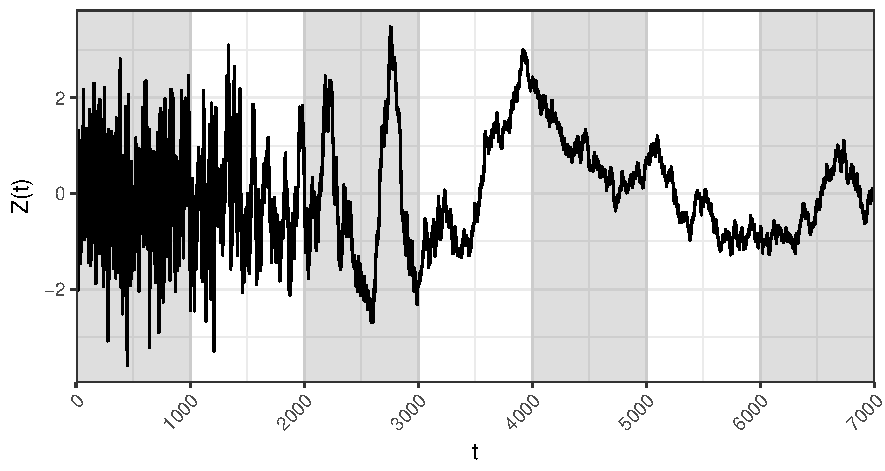
\includegraphics[width=0.9\linewidth]{./scripts_graf_res/proceso_Z.pdf}
\caption[Realización de un proceso estocástico, usado para ejemplificar la prueba de PSR.]{Realización del proceso estocástico $\{Z(t)\}_{t\in\R}$, usado para ejemplificar el procedimiento de la prueba de PSR.
Las regiones sombreadas indican la segmentación usada para dicha prueba.}
\label{fig:lazy21}
\end{figure}

Una vez expuestas las características del proceso $\{Z(t)\}_{t\in\R}$, pero no su espectro evolutivo, se procede a aplicarle la prueba de PSR.

\subsubsection{Primer ejemplo}

Como primer paso se calcula el estimador de doble ventana, $\widehat{h}$, según la definición \ref{estimador_doble_ventana}; este estimador será calculado en una malla de puntos en el tiempo y las frecuencias.
%
%De manera concreta se calcula a  dicho estimador es calculado
para una malla de puntos en el tiempo y las frecuencias.
%
De manera concreta en este ejemplo,
la malla es construida usando $\Delta_t = 1000$ y $\Delta_\omega=50$,
% --correspondientes a $\Delta_t = 1$ y $\Delta_\omega = \nicefrac{\pi}{200}$ .
con un total de 35 puntos.
%
%En la figura ???...
%
Por simplicidad, conviene escribir nuevamente la expresión para $\widehat{h}$
\begin{equation}
\widehat{h}(\omega, t) = \sum_{u=T-t}^t w_\tau (u) \abso{U(\omega,t-u)}^{2}
\end{equation}
donde
\begin{equation}
U(t) = \sum_{u=T-t}^t g(u) X(t-u)
\end{equation}
%
En este ejemplo particular, se usa la ventana de Bartlett-Priestley, $k_\text{BP}$, para cubrir el papel de $g$ y $w_\tau$; esta función es tomada del cuadro \ref{ventanas} y
%tomada de la tabla \ref{ventanas} y 
escalada adecuadamente.
\begin{equation}
g_\tau(u) = w_\kappa(u) = \frac{1}{G_{\text{BP}}} k_{\text{BP}}\left( \nicefrac{u}{500} \right)
\end{equation}
donde
%\begin{align}
%k_{\text{BP}} (u) &= \begin{cases}
%\frac{3}{\left( \pi u \right)^2} 
%\left[ 
%\frac{\SEN{\pi u}}{\pi u} - \COS{\pi u} \right] &, \abso{u} 
%\leq 1 \\
%0 &, \text{otro caso}
%\end{cases} \\
%G_{\text{BP} &= \intR k_{\text{BP}}\left( \nicefrac{u}{500} \right) du
%\end{align}

\begin{equation}
k_{\text{BP}} (u) = \begin{cases}
\frac{3}{\left( \pi u \right)^2} 
\left[ 
\frac{\SEN{\pi u}}{\pi u} - \COS{\pi u} \right] &, \abso{u} 
\leq 1 \\
0 &, \text{otro caso}
\end{cases}
\end{equation}
\begin{equation}
G_{\text{BP}} = \intR \left[ k_{\text{BP}}\left( \nicefrac{u}{500} \right) \right]^2 du
\end{equation}

Bajo estas instrucciones es claro cómo calcular los valores de
% hacer los cálculos para obtener 
$\widehat{h}$ y
%, y posteriormente 
$Y = \log\left( \widehat{h} \right)$; estos valores se muestran en el cuadro \ref{tab:valores_psr}.
%
Con fines de claridad, en la figura \ref{fig:proceso_psr} se enfatiza esquemáticamente la interpretación que tienen 
%el logaritmo del espectro evolutivo, calculado para algunos tiempos en el tiempo y las frecuencias (en ese orden).
dichas cantidades.
%En la figura \ref{fig:proceso_psr} se muestra un bosquejo de cómo 

\begin{table}
\caption{Promedios del estimador $Y$ para el primer ejemplo}
\centering
\begin{tabular}{lrrrrrrr}
\toprule
      & \multicolumn{6}{l}{Frecuencia $\omega_i$} \\
\cmidrule{2-7}
      & $j=1$  & $j=2$   & $j=3$   & $j=4$   & $j=5$   & $j=6$   & $\widehat{\alpha_i}$ \\ 
\midrule
$i=1$ & -4.504 & -5.328  & -8.623  & -6.393  & -8.953  & -9.340  & 2.155  \\
$i=2$ & -1.418 & -7.526  & -8.463  & -11.453 & -9.392  & -9.381  & 1.406  \\
$i=3$ & -1.315 & -9.812  & -10.681 & -11.370 & -12.126 & -11.837 & -0.179 \\
$i=4$ & 1.462  & -9.852  & -10.176 & -10.732 & -11.823 & -11.880 & 0.511  \\
$i=5$ & -1.159 & -11.056 & -12.269 & -14.145 & -12.297 & -12.965 & -1.304 \\
$i=6$ & 0.221  & -10.473 & -11.111 & -12.568 & -13.392 & -14.044 & -0.883 \\
$i=7$ & -2.713 & -11.255 & -12.739 & -13.670 & -13.560 & -12.373 & -1.707 \\
$\widehat{\beta_j}$
      & 7.998  & 0.016   & -1.235  & -2.131  & -2.304  & -2.344  & 
%      -9.345 
      \\ 
\bottomrule
\end{tabular}
\label{tab:valores_psr}
\end{table}

A partir de los datos del cuadro \ref{tab:valores_psr} efectúa el ANOVA de dos vías usando los estimadores descritos en el cuadro \ref{cantidades_psr}.
%
Primeramente se calcula el promedio global $\widehat{\mu} = -9.345$;
posteriormente se calculan $\widehat{\alpha_i}$ y $\beta_j$ para $i=1,\dots, 7$ y $j=1,\dots, 6$, respectivamente. 
%
Después se calculan las sumas de cuadrados, estas últimas reportadas en el cuadro \ref{tab:ejemplo_gl}.
%
Finalmente se calculan los estadísticos de prueba
\begin{align}
F_{I+R} &= \frac{\nicefrac{S_{I+R}}{(I-1)(J-1)}}{\nicefrac{S_0}{(IJ-1)}} = 0.589 \\
F_{T} &= \frac{\nicefrac{S_{T}}{(I-1)}}{\nicefrac{S_0}{(IJ-1)}} = 0.112
\end{align}

Se calcula el p-valor de los estadísticos de prueba comparándolos con las distribuciones de los estadísticos: $F$ de Fisher con $(6,34)$ y $(30,34)$ grados de libertad, respectivamente.
%
Como se mencionó, 
%para los fines de la prueba de PSR la decisión es \textit{opuesta} a los ANOVA usuales donde la hipótesis nula es igualdad de medias; 
la decisión de la prueba de PSR en base a los p-valores es \textit{opuesta} a los ANOVA usuales:
como hay
%los datos aportan 
suficiente información para afirmar que $F_{I+R} \neq 0$, entonces se acepta 
%--más bien, no se rechaza-- 
que el proceso es no-estacionario.
%
Cabe recalcar que la decisión sobre estacionariedad se hace aún sin consultar a $F_T$.
%, ya que éste último está sujeto a que se rechace la hipótesis intermedia.


\begin{table}
\centering
\caption{ANOVA de la prueba PSR para el primer ejemplo}
\begin{tabular}{llrrrrrr}
\toprule
\multicolumn{2}{l}{Efecto}
                        & GL & Total   & Promedio & $F$   & $p$     & $1-p$   \\
\midrule
$S_T$     & Tiempo      & 6  & 73.834  & 12.306   & 0.589 & 0.26290 & 0.73710 \\
$S_F$     & Frecuencia  & 5  & 565.891 & 113.178  & 5.420 & 0.99935 & 0.00065 \\
$S_{I+R}$ & Interacción & 30 & 70.247  & 2.342    & 0.112 & 0.00000 & 1.00000 \\
$S_0$     & Total       & 34 & 709.972 & 20.882   &       &         &         \\
\bottomrule
\multicolumn{5}{l}{GL = Grados de libertad}
\end{tabular}
\label{tab:ejemplo_gl}
\end{table}


\begin{figure}
\centering
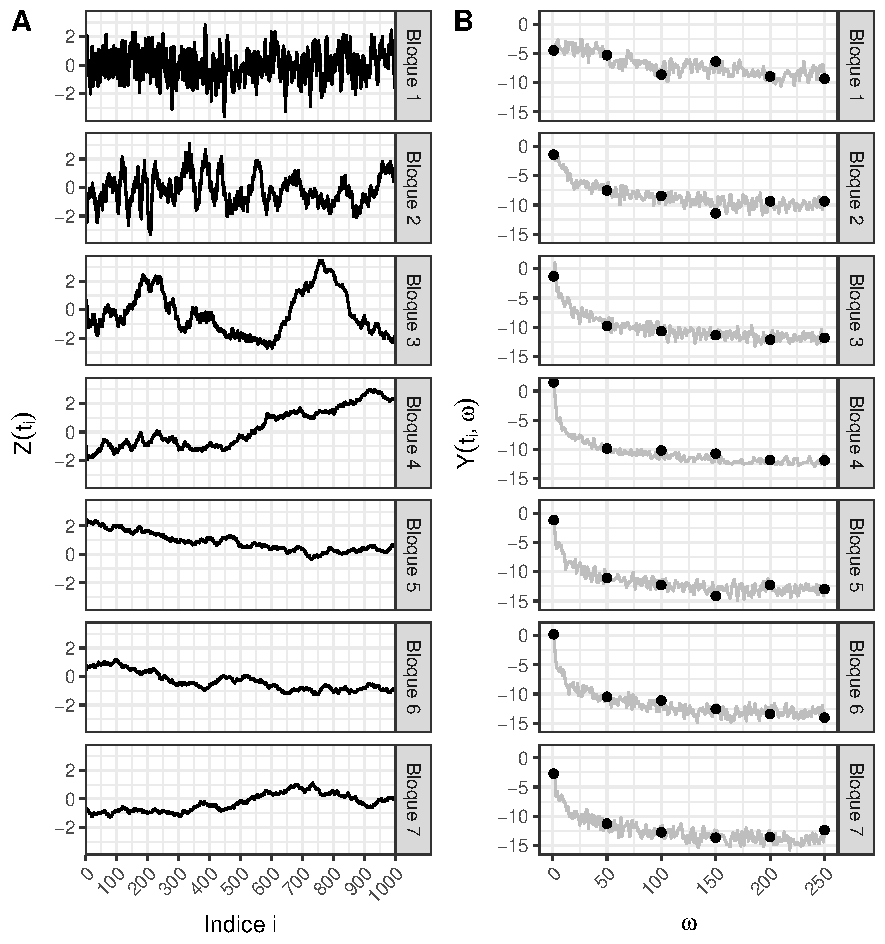
\includegraphics[width=\linewidth]{./scripts_graf_res/proceso_Z_fragmentado_doble.pdf}
\caption{Algunos pasos en el cálculo de $Y$, el logaritmo del estimador de doble ventana, sobre la malla de puntos $\{ t_1, t_2, \dots, t_I\} \times \{\omega_1, \omega_2, \dots, \omega_J\}$.
\textbf{A.}
Realización del proceso estocástico $\{Z(t)\}_{t\in\R}$, fragmentada en bloques de longitud $\Delta_t$. 
%
Los puntos en el $i$--ésimo bloque son usados para calcular $Y_{i,j}$
%el estimador de doble ventana 
en los puntos $\omega_1, \omega_2, \dots, \omega_J$.
% $(t_i,\omega_1), (t_i,\omega_2), \dots, (t_i,\omega_J)$.
\textbf{B.}
Estimador $Y$, calculado para los bloques definidos anteriormente.
% calculado sobre la malla de puntos $(t_i,\omega_j)$.
%
Por fines expositivos
%Para ser más explicativo 
se grafica a $Y(t_i,\bullet)$ para diferentes valores de $\omega$, y posteriormente se marcan con puntos los valores correspondientes a la malla.}
\label{fig:proceso_psr}
\end{figure}

Para el análisis anterior se usó una cantidad muy baja de puntos con el fin de ilustrar claramente cómo son procesados estos datos.
%
Una versión más realista requiere usar la mayor cantidad de puntos posibles en el tiempo y las frecuencias, pero que sean tales que se cumplan las aproximaciones usadas;
en principio no existen criterios para hallar estos parámetros de forma óptima, al menos no si las propiedades de los datos son desconocidas.

En la implementación del comando \texttt{stationarity} se sugiere que el número de bloques sea
$\entero{\log_2(N)}$, con $N$ el número total de puntos considerados y $\entero{\bullet}$ la función parte entera, y $\Delta_\omega=6$.

%Para comparar resultados con dicha implementación se repite el análisis usando 12 bloques, cada uno con 583 puntos ($\Delta_t=583$) e ignorando 4 observaciones.
%
%Estos resultados se muestran en el anexo 

%En la figura \ref{fig:farol} se muestran, con fines meramente ilustrativos, la realización $Z(t)$ y los estimadores $\log\left(\abso{U}^2\right)$ y $\log\left( \widehat{h} \right)$ calculados para todos los puntos posibles; en este ejemplo es claro que el segundo tiene menor varianza que el primero.
%%
%%En contraparte, en las figuras ?? ?? ?? se muestra, respectivamente, las observaciones fragmentadas para evaluar el espectro evolutivo y los estimadores calculados para tales fragmentos; se han mostrados los estimadores evaluados para una gran cantidad de puntos en las frecuencias, los puntos en la malla son los siguientes:

%\begin{figure}
%\centering
%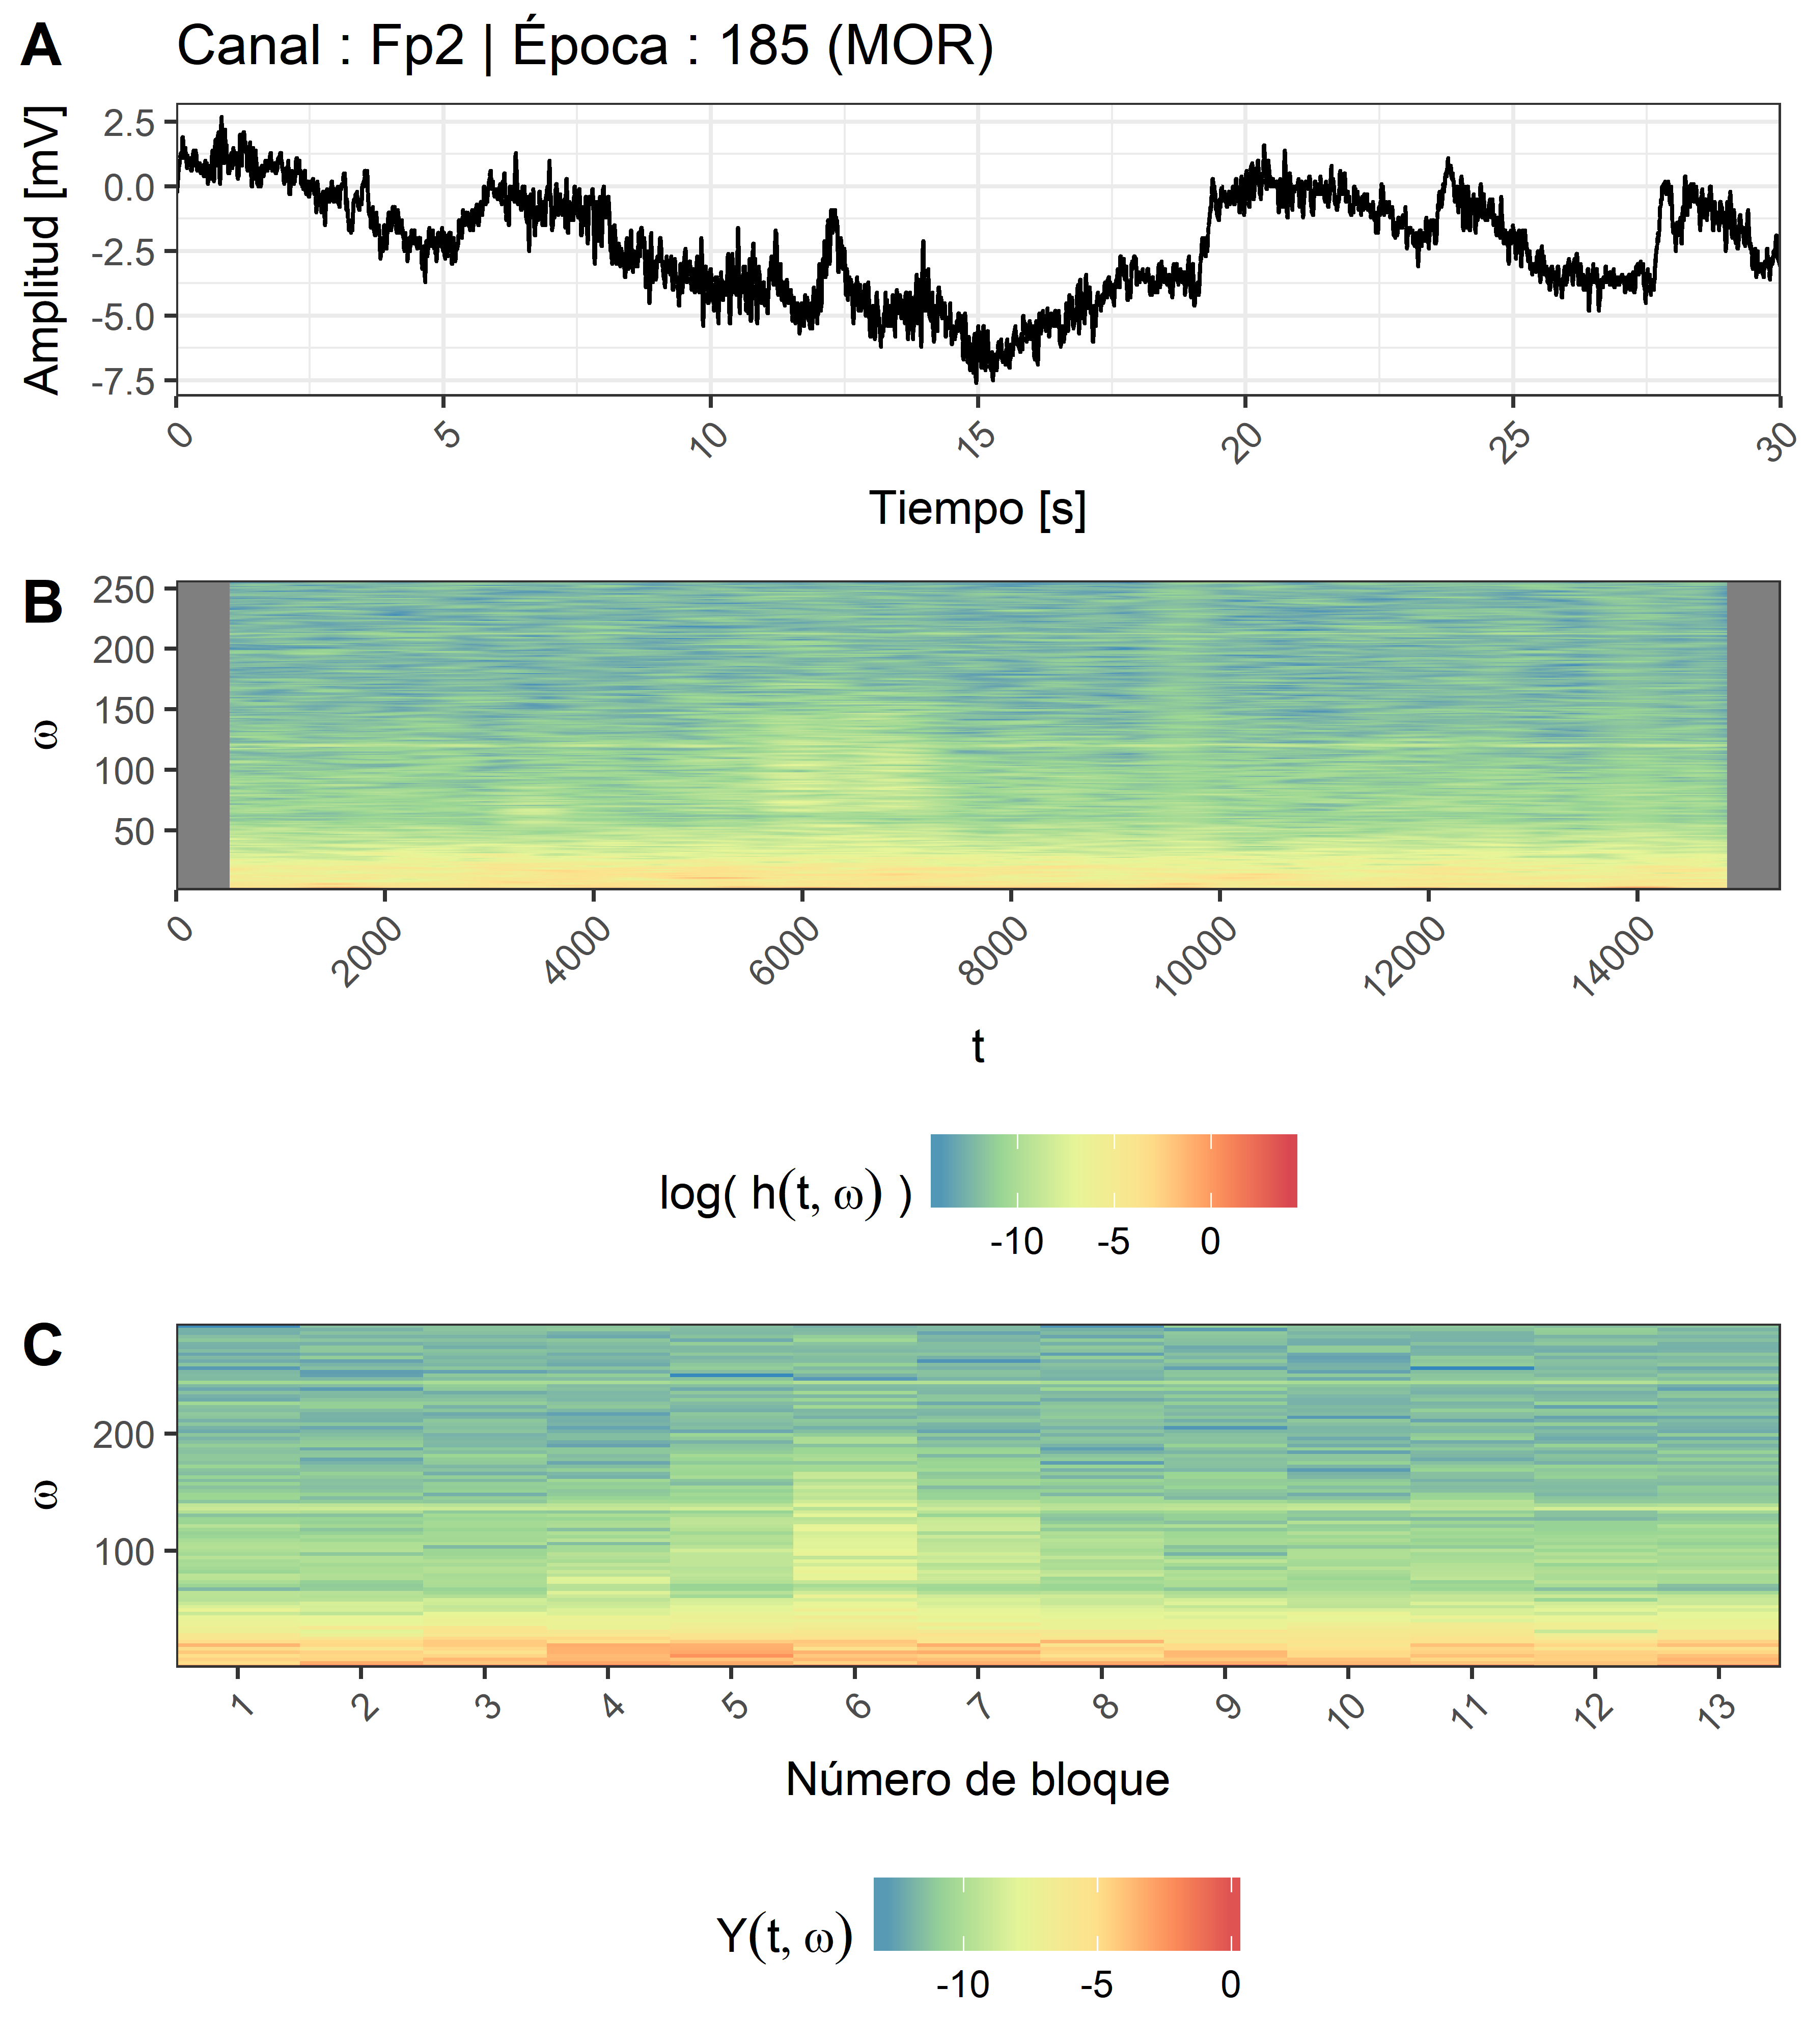
\includegraphics[width=\linewidth]{./scripts_graf_res/proceso_Z_varios_v2.png}
%\caption{Logaritmo del espectro evolutivo para el proceso $\{Z(t)\}_{t\in\R}$, calculado usando el estimador de doble ventana a partir de una realización. 
%\textbf{A.} Realización del proceso, $Z(t)$, generada en el intervalo $[-3.5,3.5]$ con frecuencia de muestreo $\Delta_Z=\nicefrac{1}{1000}$ y posteriormente reindexada para usar $\Delta_Z=1$.
%%\textbf{B.} Estimador de una ventana, $\abso{U}^2$, al cual se aplicó la función $\log$. 
%%Como se mostró en la sección ?, es un estimador aproximadamente insesgado e inconsistente. 
%\textbf{B.} Estimador de doble ventana, $h$, al cual se aplicó la función $\log$. 
%%Como se mostró en la sección ?, es un estimador aproximadamente insesgado y consistente.
%\textbf{C.} Logaritmo del estimador de doble ventana, $Y$, calculado usando la implementación de la prueba de PSR (comando \texttt{stationarity}) en el paquete \texttt{fractal} \cite{R_fractal}.
%}
%\label{fig:farol}
%\end{figure}

\subsubsection*{Segundo ejemplo}

Como segundo ejemplo se usa un fragmento arbitrario de registro de PSG; en particular se ha usado una época\footnote{La palabra `época' es usada como sinónimo de `fragmento de registro' por concordancia con la literatura sobre registros electrofisiológicos.} de 30 segundos de duración, correspondiente a la derivación Fp2 registrada en el participante MHJ durante sueño MOR; en la sección \ref{sec:eeg} se explica a detalle el significado de estos términos.
%
El registro fue efectuado usando una frecuencia de muestreo de 512 Hz ($\Delta_X =\nicefrac{1}{512}$), de modo que se contemplan 15,360 puntos; éstos mismos puntos son graficados en la figura \ref{fig:lazy22}.

Cabe destacar que este fragmento de registro no fue elegido para representar alguna característica en particular sino, 
%que, todo lo contrario, se presenta para ilustrar las características \textit{usuales} de un fragmento de registro de PSG durante el sueño MOR.
más bien, el comportamiento general de los registros de PSG durante sueño MOR.

\begin{figure}
\centering
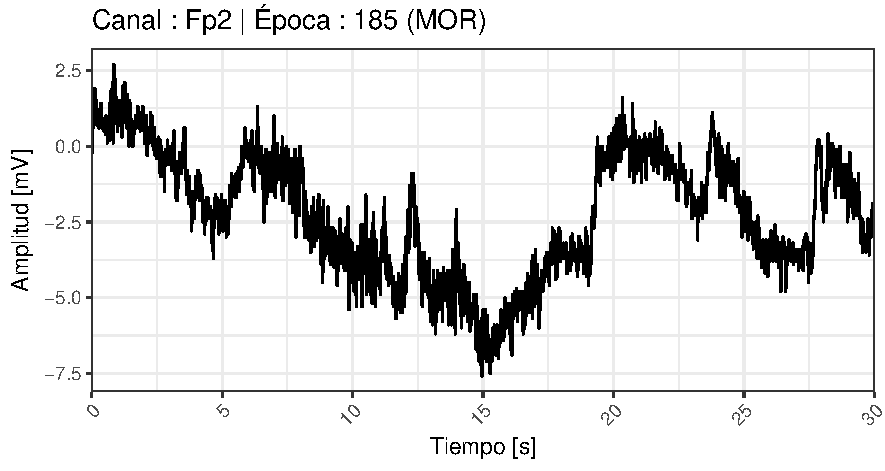
\includegraphics[width=.9\linewidth]{./scripts_graf_res/psg.pdf}
\caption[Fragmento de registro de PSG, usado para ejemplificar la prueba de PSR.]{Fragmento de registro de PSG, usado para ejemplificar el procedimiento de la prueba de PSR.
El fragmento, referido como época, corresponde a 30 segundos registradas con una frecuencia de muestreo de 512 Hz; posteriormente fue reindexado.}
\label{fig:lazy22}
\end{figure}

El estimador $Y$ es calculado de la misma forma que en el ejemplo anterior; en esta ocasión simplemente se reportan los resultados en las tablas \ref{tab:valores_psr_2} y \ref{tab:ejemplo_gl_2}.
%
Para estos datos se calcula que $\widehat{\mu} = -9.265$; aunque este dato no se reporta en las tablas, efectivamente es importante. 

Tras revisar los estadísticos de prueba se decide, como se esperaba intuitivamente, que el fragmento de registro es no-estacionario.
%
%Conviene comentar, con base a la figura \ref{fig:lazy21}, que el registro tiene una apariencia similar a 

\begin{table}
\caption{Promedios del estimador $Y$ para el segundo ejemplo}
\centering
\begin{tabular}{lrrrrrrr}
\toprule
      & \multicolumn{6}{l}{Frecuencia $\omega_i$} \\
\cmidrule{2-7}
      & $j=1$  & $j=2$   & $j=3$   & $j=4$   & $j=5$   & $j=6$   & $\widehat{\alpha_i}$ \\ 
\midrule
$i=1$ & -0.858 & -9.903  & -11.987 & -12.942 & -11.632 & -11.962 & -0.616 \\
$i=2$ & 1.709  & -10.475 & -11.567 & -12.401 & -12.267 & -13.068 & -0.413 \\
$i=3$ & 3.701  & -8.860  & -9.321  & -10.844 & -11.392 & -12.501 & 1.062  \\
$i=4$ & 3.236  & -9.175  & -10.387 & -12.345 & -14.106 & -12.106 & 0.118  \\
$i=5$ & 1.474  & -10.461 & -11.116 & -12.332 & -12.835 & -13.399 & -0.513 \\
$i=6$ & 1.442  & -9.301  & -10.257 & -10.947 & -12.500 & -11.852 & 0.362  \\
$\widehat{\beta_j}$
     & 11.049 & -0.431  & -1.508  & -2.704  & -3.190  & -3.216  &         \\
\bottomrule
\end{tabular}
\label{tab:valores_psr_2}
\end{table}

\begin{table}
\centering
\caption{ANOVA de la prueba PSR para el segundo ejemplo}
\begin{tabular}{llrrrrrr}
\toprule
\multicolumn{2}{l}{Efecto}
                        & GL & Total   & Promedio & $F$   & $p$     & $1-p$   \\
\midrule
$S_T$     & Tiempo      & 5  & 12.520  & 2.504   & 0.093 & 0.00721 & 0.99279 \\
$S_F$     & Frecuencia  & 5  & 914.235 & 182.847 & 6.774 & 0.99984 & 0.00016 \\
$S_{I+R}$ & Interacción & 25 & 17.998  & 0.720   & 0.027 & 0.00000 & 1.00000 \\
$S_0$     & Total       & 35 & 944.753 & 26.993  &       &         &         \\
\bottomrule
\multicolumn{5}{l}{GL = Grados de libertad}
\end{tabular}
\label{tab:ejemplo_gl_2}
\end{table}

%\subsubsection*{Comentarios sobre la implementación}

%%%%%%%%%%%%%%%%%%%%%%%%%%%%%%%%%%%%%%%%%%%%%%%%%%%%%%%%%%%%%%%%%%%%%%%%%%%%%%%%%%%%%%%%%%%%%%%%%%%
%%%%%%%%%%%%%%%%%%%%%%%%%%%%%%%%%%%%%%%%%%%%%%%%%%%%%%%%%%%%%%%%%%%%%%%%%%%%%%%%%%%%%%%%%%%%%%%%%%%

\section{Estacionariedad local}
\label{sec:est_local}

%Se considera que la técnica de EEG fue inventada en la década de 1920 por el fisiólogo Hans Berger, quien descubrió que ésta es \textit{sensible} a cambios en la actividad mental como la atención sostenida o el parpadeo voluntario.
%%
%Desde entonces se estableció que hay una \textit{conexión} entre el funcionamiento de la mente y los fenómenos eléctricos en el cerebro.

Conviene destacar que el objetivo central del presente trabajo es utilizar las herramientas descritas anteriormente (en especial la prueba de PSR) sobre registros de PSG en adultos mayores.
%
Para que los análisis sean significativos, desde el punto de vista fisiológico, deben resaltarse algunos \textit{comportamientos} esperados; en otras palabras, algunas propiedades de estas señales  se deben considerar conocidas a priori, con base a lo que se ha reportado en la literatura.
%
De forma particular, se ha propuesto que el cerebro es un mecanismo con una gran \textit{complejidad} asociada \cite{Werner09}.

Bajo este contexto se entiende a la complejidad como la presencia de características propias de un conjunto de elementos, 
%que afectan de forma diferente al conjunto de elementos y a los elementos por separado.
que inducen {estados} independientes de los elementos individuales, pero que dependen \textit{críticamente} de parámetros macroscópicos.
%
Un ejemplo sencillo es la solidificación del agua, que depende principalmente de la temperatura y permite múltiples estados de equilibrio macroscópicos (la forma del hielo) que no están determinados por las partículas de agua; cerca de la temperatura de congelamiento el agua pasa de líquido a sólido, sin permitir estados intermedios.

La complejidad del cerebro se deduce de la existencia de múltiples niveles de organización, que corresponden a comportamientos cualitativamente diferentes --los cuales deben ser modelado usando herramientas que respeten tales diferencias.
%
Como ejemplo pueden mencionarse los campos eléctricos inducidos por neuronas individuales y por grandes conjuntos de neuronas; estos dos fenómenos están estrechamente relacionados de manera intuitiva, pero cualitativamente son abismalmente diferentes.
%
En el libro \textit{``Mathematical Foundations of Neuroscience"}, por G. Bard Ermentrout \cite{Ermentrout10}, se describe a detalle cómo los potenciales para neuronas pueden modelarse satisfactoriamente mediante el sistema de ecuaciones diferenciales de Hodgkin--Huxley; en contraparte, los \textit{potenciales de campo} responden mejor al sistema de ecuaciones diferenciales estocásticas Wilson--Cowan.

Para el caso muy concreto del EEG, se ha propuesto la complejidad de la actividad eléctrica cerebral se traduce en la {orquestación} de múltiples estados de actividad a lo largo del tiempo \cite{kaplan2000application}. 
%
En otras palabras, el EEG es una señal compleja que está formada por una gran variedad de fragmentos \textit{simples}; en concreto, se espera que estos fragmentos sean débilmente estacionarios.
%
Concordando con la definición formal hecha sobre el tema por Rainer Dahlhaus \cite{Dahlhaus97}, este fenómeno será referido como \underline{estacionariedad local}.

Bajo el supuesto de la estacionariedad local el EEG es un fenómeno globalmente heterogéneo pero localmente homogéneo; en consecuencia el EEG es globalmente no-estacionario, pero es posible segmentarlo en fragmentos que son débilmente estacionarios.
%
Dentro de esta línea de pensamiento se espera que los fragmentos de EEG débilmente estacionarios --o que clasifiquen como estacionarios según la prueba de PSR, en concreto-- se \textit{agrupen} replicando algún nivel de organización.

\begin{figure}
\centering
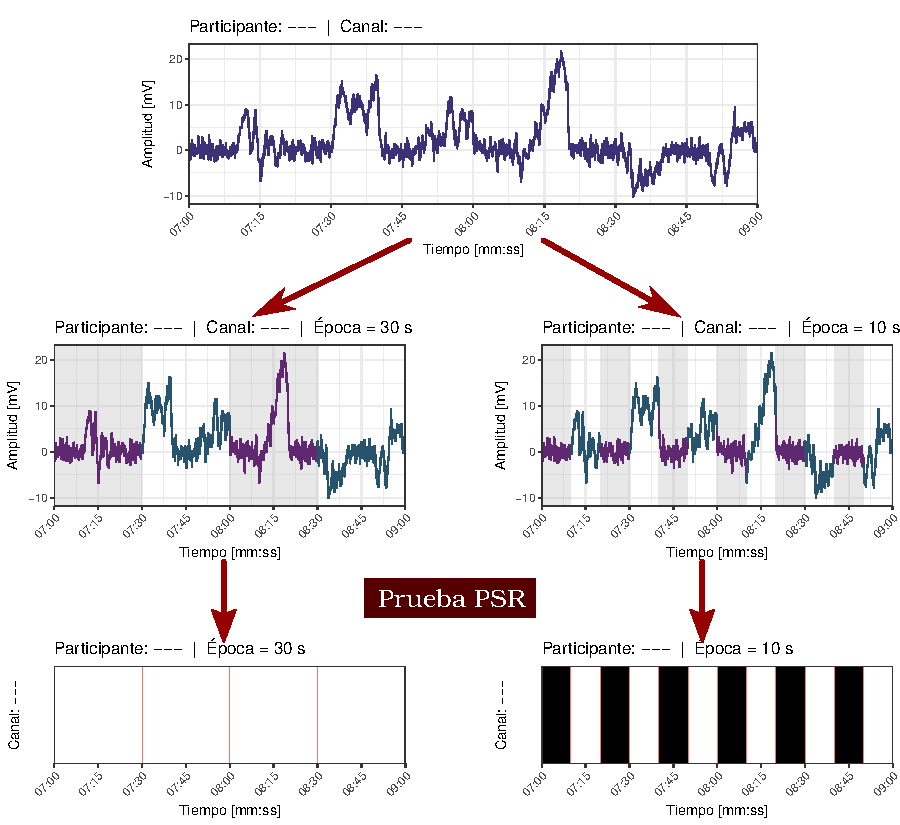
\includegraphics[width=\linewidth]{./img_diagramas/epocas_diferentes_v3.pdf}
\caption[Efecto esperado del tamaño de ventana sobre la clasificación de estacionariedad, bajo el supuesto de estacionariedad local]{Efecto esperado del tamaño de ventana sobre la clasificación de estacionariedad, bajo el supuesto de estacionariedad local.
%
Suponiendo que la señal es heterogénea, pero que está \textit{compuesta} por múltimples fragmentos homogéneo de duración corta, entonces al disminuir el tamaño de ventana se espera \textit{hallar} con mayor frecuencia estos fragmentos homogéneos.
%
Adaptado de \cite{FRONTIERS}.
}
\label{epocas_diferentes}
\end{figure}

De manera pragmática y de acuerdo a los protocolos (ver más adelante), los registros de PSG son segmentados en ventanas sin traslape con una duración fija decidida a priori.
%
Así entonces, se espera que el efecto de la estacionariedad local se más notorio al cambiar el tamaño de tales segmentos; este procedimiento se ilustra en la figura \ref{epocas_diferentes}, así como el efecto esperado sobre la clasificación de estacionariedad.


Cabe destacar que bajo este supuesto, surge la pregunta sobre hasta qué punto es posible es posible modelar efectivamente al EEG como señales aleatorias con propiedades \textit{simples}.
%
En varios trabajos pioneros \cite{Cohen77,Kawabata73,McEwen75,Sugimoto78} se demuestra experimentalmente que el EEG puede considerarse estacionario si se usan segmentos de hasta 20 segundos, e incluso se sugiere que esta cantidad puede cambiar para personas con daños neuronales.
%
Esta pregunta es explorada en el presente trabajo repitiendo la prueba de PSR para diferentes tamaños de ventana.
%
Es importante considerar, debido a la --posible-- variabilidad en el tiempo, el efecto de tomar una cantidad menor de puntos es cualitativamente diferente al efecto de, por ejemplo, considerar una frecuencia de muestreo menor.

Por ejemplo, considérese al primer ejemplo de la sección anterior, el proceso $\{Z(t)\}$, que es aproximadamente un proceso ruido blanco para $t\ll 0$ y aproximadamente un proceso medias móviles para $t \gg 0$; este proceso es localmente estacionario por diseño.
%
En la figura \ref{lazy_fin} se efectúa esta clasificación repetida para diversos tamaños de ventana, revelando que los fragmentos pequeños son clasificados como estacionarios.
%
Este efecto era de esperarse por la descripción de estacionariedad local: un fenómeno que es globalmente heterogéneo pero que está \textit{compuesto} por fragmentos homogéneos.

\begin{figure}
\centering
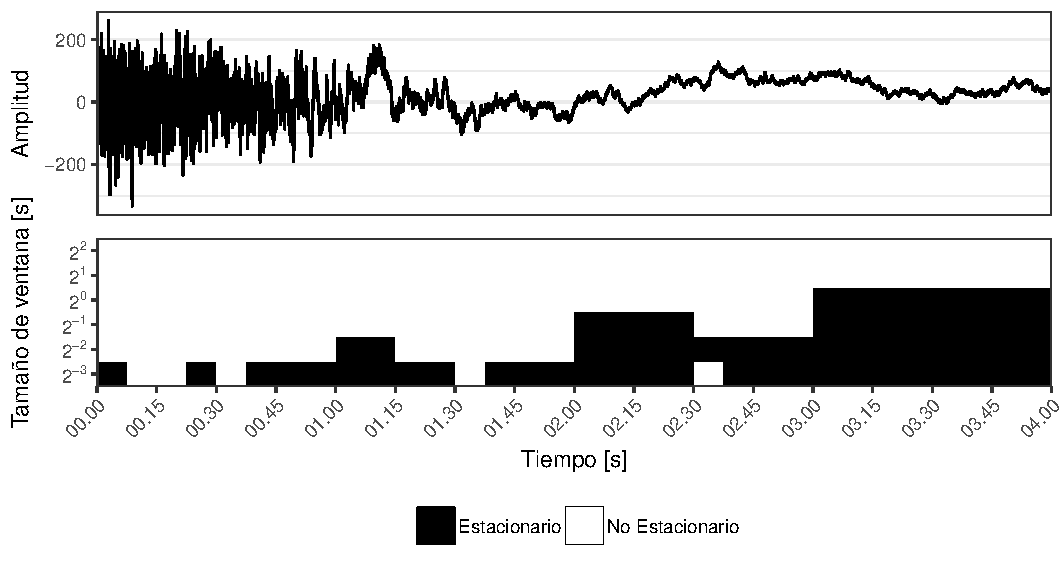
\includegraphics[width=\linewidth]{./scripts_graf_res/stat_local_artificial.pdf}
\caption[Efecto de la estacionariedad local sobre la clasificación repetida de estacionariedad, según la prueba de Priesltey-Subba Rao, usando diferentes tamaños de ventana.]{Efecto de la estacionariedad local sobre la clasificación repetida de estacionariedad, según la prueba de Priesltey-Subba Rao, usando diferentes tamaños de ventana.
%
En la parte superior se muestra a la señal usada ejemplo, una realización para un proceso estocástico localmente estacionario cuyas propiedades se describen en el texto.
%
En la parte inferior se muestran las ventanas usadas para segmentar la señal, las cuales fueron coloreadas según si tal fragmento de señal fue clasificado como estacionario.
%
Puede notarse cómo la señal es efectivamente estacionaria, pero algunos fragmentos pequeños son clasificados como estacionarios.
}
\label{lazy_fin}
\end{figure}

Posteriormente se replica este análisis para los registros de PSG en el total de su duración.
%
Los tamaños de ventana se tomaron de la forma $30 \times 2^{n}$ segundos, por compatibilidad con las ventanas de 30 segundos (recomendación protocolaria de la AASM); para más detalles sobre el procedimiento, ver la sección \ref{sec:analisis_registro}. 
%
Conviene mencionar que esta metodología es similar a aquella usada por McEwen en 1975 \cite{McEwen75}.
%, para lo cual la clasificación de estacionariedad se repite usando ventanas de diferente tamaño; 
%%
%P.

%%%%%%%%%%%%%%%%%%%%%%%%%%%%%%%%%%%%%%%%%%%%%%%%%%%%%%%%%%%%%%%%%%%%%%%%%%%%%%%%%%%%%%%%%%%%%%%%%%%
%%%%%%%%%%%%%%%%%%%%%%%%%%%%%%%%%%%%%%%%%%%%%%%%%%%%%%%%%%%%%%%%%%%%%%%%%%%%%%%%%%%%%%%%%%%%%%%%%%%
%%%%%%%%%%%%%%%%%%%%%%%%%%%%%%%%%%%%%%%%%%%%%%%%%%%%%%%%%%%%%%%%%%%%%%%%%%%%%%%%%%%%%%%%%%%%%%%%%%%
%%%%%%%%%%%%%%%%%%%%%%%%%%%%%%%%%%%%%%%%%%%%%%%%%%%%%%%%%%%%%%%%%%%%%%%%%%%%%%%%%%%%%%%%%%%%%%%%%%%

%%%%%%%%%%%%%%%%%%%%%%%%%%%%%%%%%%%%%%%%%%%%%%%%%%%%%%%%%%%%%%%%%%%%%%%%%%%%%%%%%%%%%%%%%%%%%%%%%%%
%%%%%%%%%%%%%%%%%%%%%%%%%%%%%%%%%%%%%%%%%%%%%%%%%%%%%%%%%%%%%%%%%%%%%%%%%%%%%%%%%%%%%%%%%%%%%%%%%%%
%%%%%%%%%%%%%%%%%%%%%%%%%%%%%%%%%%%%%%%%%%%%%%%%%%%%%%%%%%%%%%%%%%%%%%%%%%%%%%%%%%%%%%%%%%%%%%%%%%%
%%%%%%%%%%%%%%%%%%%%%%%%%%%%%%%%%%%%%%%%%%%%%%%%%%%%%%%%%%%%%%%%%%%%%%%%%%%%%%%%%%%%%%%%%%%%%%%%%%%

\chapter{Deterioro cognitivo y sueño}

En este capítulo se exponen varios temas para poder entender adecuadamente al sujeto de estudio (registros de PSG en adultos mayores), así como el contexto y la motivación para su estudio (el Posible Deterioro Cognitivo Leve, PDCL, en adultos mayores).
%
Se responden, de manera muy breve, las siguientes preguntas:
\begin{itemize}
\item ¿Qué es el Deterioro Cognitivo Leve y cómo se diagnostica?
\item Clínicamente, ¿qué es el sueño y cómo se estudia?
\item ¿Cómo se relacionan el Deterioro Cognitivo Leve y el sueño?
\end{itemize}

Para simplificar la exposición, se considera a la Electroencefalografía como a la técnica principal para el estudio de la actividad cerebral;
%
con la misma intención, se describe primero al sueño (desde el punto de vista clínico) y posteriormente su posible utilidad como marcador para el DCL.

El lector interesado en una exposición amplia sobre técnicas para el estudio del cerebro, puede referirse al libro \textit{``Medical Instrumentation. Applications and Design"} por John Webster \cite{Webster}; en contraparte, para obtener más información sobre el EEG es recomendable el libro \textit{``Electroencephalography: Basic Principles, Clinical Applications, and Related Fields"} por Ernst Niedermeyer \cite{niedermeyer}.
%
Para indagar más sobre las pruebas neuropsicológicas y su uso diagnóstico, se recomienda el libro \textit{``Guía para el diagnóstico neuropsicológico"} por Ardila y Ostrosky \cite{Ardila12}.
%
Si se desean revisar a detalle los protocolos para registrar la PSG, o aquellos para clasificar las etapas de sueño, debe consultarse el Manual de la AASM \cite{AASM07}.
%
Para aprender más sobre el sueño, así como los procesos fisiológicos y psicológicos asociados, puede consultarse el libro \textit{``Psicofisiología del sueño"} de Corsi-Cabrera \cite{Corsi1983}.

%%%%%%%%%%%%%%%%%%%%%%%%%%%%%%%%%%%%%%%%%%%%%%%%%%%%%%%%%%%%%%%%%%%%%%%%%%%%%%%%%%%%%%%%%%%%%%%%%%%
%%%%%%%%%%%%%%%%%%%%%%%%%%%%%%%%%%%%%%%%%%%%%%%%%%%%%%%%%%%%%%%%%%%%%%%%%%%%%%%%%%%%%%%%%%%%%%%%%%%

\section{Deterioro Cognitivo Leve}
\label{seccion:dcl}

El envejecimiento es determinado por una serie de procesos moleculares, celulares, fisiológicos y psicológicos que conducen directamente al deterioro de funciones cognitivas, específicamente atención y memoria \cite{Park09}.
%
Como consecuencia, los \textbf{adultos mayores} son especialmente propensos al deterioro cognitivo; por precisión, en lo siguiente se usará el término \textit{adulto mayor} para referirse a individuos con 60 o más de edad años.
%
Cabe destacar que la funcionalidad del adulto mayor no depende meramente de la edad, sino que está relacionada con el estilo de vida, los factores de riesgo, el acceso a la educación y las acciones para el cuidado de la salud realizadas en edades más tempranas \cite{Sanhueza14}.
 
La \textbf{demencia}, considerada como el estado más grave del deterioro cognitivo, es definida en el Manual Diagnóstico y Estadístico de Trastornos Mentales (DSM-V, por sus siglas en inglés y la versión consultada) como sigue:
\begin{quote}
``Un síndrome que consiste en el desarrollo de déficits cognoscitivos suficientemente graves como para interferir significativamente en las actividades laborales y sociales, respecto al nivel de actividad previo.\\
%
Los sujetos con demencia tienen una baja capacidad para aprender información nueva y suelen olvidar lo aprendido anteriormente, siendo éste el síntoma más prominente."  \cite{DCM5}
\end{quote}

Hasta el momento se considera que la demencia es irreversible, y no se han identificado curas \cite{PlanAlzheimer04}. 
%
Debido a ello, ha surgido un gran interés en definir y diagnosticar sus etapas tempranas. 
%
El diagnóstico temprano es importante para un tratamiento adecuado que revierta o desacelere el avance de este síndrome \cite{Knopman01}.

Bajo esta línea de pensamiento se considera al \textbf{Deterioro Cognitivo Leve} (DCL) como una etapa precursora de la demencia, y que es definida como sigue: 
\begin{quote}
``Una alteración adquirida y prolongada de una o varias funciones cognitivas, que no corresponde a un síndrome focal y no cumple criterios suficientes de gravedad para ser calificada como demencia." \cite{Robles02}
\end{quote}

Para fines de la definición anterior, se entiende por \textit{síndrome focal} al daño en una estructura nerviosa específica, cuya causa es conocida (como una hemorragia o una embolia) y cuyo inicio sea inmediato y evidente. 

El DCL puede detectarse por medio de diversos métodos, que pueden ser complementarios entre sí. 
%
La forma de detección más simple es la percepción de fallas en la memoria por parte del individuo o de otro. 
%
La percepción subjetiva del deterioro cognitivo \textit{esperado} por el envejecimiento provoca que esta forma de detección sea poco fiable.
%
Una alternativa más {formal} consiste en la entrevista clínica de un especialista, la aplicación de cuestionarios sobre dificultades en la memoria, o incluso el uso de pruebas neuropsicológicas. 

En psicología, los instrumentos de medición comunes son las \textbf{pruebas neuropsicológicas}, 
entendidas como muestras de alguna conducta de interés a las que se asignan puntajes para comparar 
cuantitativamente a los sujetos \cite{Ardila12}.
%
Se considera que a través de estas herramientas es posible declarar objetivamente las deficiencias cognitivas o conductuales de los individuos, así como su severidad y características.

De forma auxiliar para el diagnóstico del DCL, se pueden efectuar análisis genéticos, químicos, de imágenes cerebral, entre otros que estudien el sistema nervioso central.
%
Se espera que dichas técnicas, en combinación con las pruebas neuropsicológicas, permitan diagnosticar más acertadamente el DCL y desentrañar los fenómenos neurobiológicos subyacentes.

Un referente ampliamente usado para el diagnóstico del DCL son los criterios para Alzheimer de la NINCDS--ADRDA, propuestos %en 1984 
por el \textit{National Institute of Neurological and Communicative Disorders and Stroke} y la \textit{Alzheimer's Disease and Related Disorders Association} 
%\cite{McKhann,Dubois07}. 
\cite{Dubois07}. 
%
Dichos criterios proporcionan protocolos para diagnosticar el Alzheimer y algunas enfermedades relacionadas (entre ellas el DCL), así como afecciones que generan síntomas similares. 
%
Desafortunadamente, las pruebas neuropsicológicas contempladas por los criterios de la NINCDS--ADRDA todavía no han sido \textit{validadas} en México, es decir que su efectividad para generar diagnósticos acertados no ha sido verificada para la población mexicana. 

Otra prueba neuropsicológica ampliamente extendida es el Mini-Mental State Examination (MMSE), propuesta por Folstein en 1975 \cite{folstein75}. %[citar mas, quiza??].
%
Sin embargo se ha reportado que, en la población mexicana, la prueba MMSE tiene baja sensibilidad para el diagnóstico de DCL en general, y baja especificidad para individuos con escolaridad muy baja o muy alta \cite{Ostrosky00}.
%
Para fines del comentario anterior, se entiende por \textit{sensibilidad} a la probabilidad de obtener verdaderos positivos, y por \textit{especificidad} a la probabilidad de obtener verdaderos negativos.

%En cambio, en estudios epidemiológicos, el Examen Cognitivo Transcultural (CCCE) y otras pruebas se han utilizado \cite{Rosales-Lagarde2016}. 
%%
%El CCCE muestra una prevalencia del 28.7 \% de deterioro cognitivo sin demencia (DCSD) que aumenta con la edad y disminuye con un nivel educativo más alto \cite{Mejia-Arango2011}. 

Una tercera opción, a la cual se ha dado gran peso en el presente trabajo, es la prueba neuropsicológica Neuropsi, desarrollada por Ostrosky y colaboradores en la Universidad Autónoma de México (UNAM) \cite{Ostrosky1999}.
%
La prueba Neuropsi ha sido validada para diversos grupos poblacionales en México, y se ha confirmado su utilidad para distinguir individuos con diverso grado de deterioro cognitivo.

En el contexto de la detección del DCL, es muy importante realizar un diagnóstico diferencial con respecto a la \textbf{pseudodemencia depresiva}, una afección que puede confundirse con el deterioro cognitivo.
%
De acuerdo al manual DSM-V, pseudodemencia depresiva se define como \textit{``un trastorno del afecto y que produce un aparente deterioro cognitivo"} \cite{DCM5}.
%
Bajo esta línea de pensamiento resulta conveniente decir que, como parte del diseño experimental, se han omitido participantes con síndromes focales, retraso mental, bipolaridad, esquizofrenia, entre otros trastornos de atención y memoria ajenos al deterioro cognitivo. 
%
Con base a lo anterior, se omite una discusión más extensa de dicho tipo de afecciones; el lector interesado puede referirse al Manual DSM-V \cite{DCM5}.

\subsection{Probable Deterioro Cognitivo Leve}

En el presente trabajo se delimita al DCL por fines de precisión, usando para ello las pruebas neuropsicológicas. 
%
Se define operativamente al \textbf{Posible Deterioro Cognitivo Leve} (PDCL) como sigue:
\begin{quote}
``Una disminución significativa de las funciones cognitivas del sujeto con respecto las típicas de su edad y nivel de educación."
\end{quote}

Para fines de la definición anterior, el desempeño de las funciones cognoscitivas en un individuo es medido usando la prueba Neuropsi \cite{Ostrosky1999}; se considera que hay un déficit cognoscitivo \textit{significativo} si la puntuación obtenida es menor al umbral predefinido para su grupo de edad y nivel de escolaridad.
%
El umbral recomendado para la prueba Neuropsi debe calcularse como la media menos 3 desviaciones estándar de los puntajes típicos para individuos de cada grupo de edad y nivel de escolaridad; estos parámetros fueron estimados para la población mexicana por Ostrosky-Solís y colaboradores \cite{Ostrosky1999}.
%
En el cuadro \ref{anexo:neuropsi}, bajo la etiqueta \textit{Deterioro cognitivo} se recaban los \textit{puntajes de corte} usados para declarar el PDCL.

La palabra \textit{`probable'} en el PDCL hace alusión a que no constituye un diagnóstico \textit{irrefutable} del DCL.
%
En este sentido, el PDCL puede interpretarse como una condición \textit{necesaria pero no suficiente} para el DCL.

%%%%%%%%%%%%%%%%%%%%%%%%%%%%%%%%%%%%%%%%%%%%%%%%%%%%%%%%%%%%%%%%%%%%%%%%%%%%%%%%%%%%%%%%%%%%%%%%%%%
%%%%%%%%%%%%%%%%%%%%%%%%%%%%%%%%%%%%%%%%%%%%%%%%%%%%%%%%%%%%%%%%%%%%%%%%%%%%%%%%%%%%%%%%%%%%%%%%%%%

\subsection{Pruebas neuropsicológicas utilizadas}
\label{seccion:pruebas}

Dentro del contexto del presente trabajo, conviene describir las pruebas que fueron usadas para detectar el PDCL en adultos mayores.
%
Según la descripción que se dio del DCL, para efectuar su diagnóstico debe verificarse que el individuo cumpla las siguientes características:
\begin{enumerate}
\item Que presente un déficit en una o varias funciones cognitivas, pero que éste no cumpla los criterios suficientes para demencia.
\item Que los déficits cognoscitivos detectados no correspondan a síndromes focales,
\item Que el individuo no presente una afección que, sin estar relacionada con el deterioro cognitivo, genere síntomas similares.
\end{enumerate}
%
Para explorar y en su caso excluir a los sujetos de la investigación, las condiciones 2 y 3 fueron investigadas mediante entrevistas con los participantes y con los resultados de las pruebas que se mencionarán a continuación.
%
%Debido a la ausencia de excepciones, la condición 3 se limitó únicamente a detectar la pseudodemencia depresiva.
%
\begin{itemize}
\item {Short Anxiety Screening Test (SAST)}\\ 
Evaluación corta para detectar trastornos depresivos y ansiosos. \cite{sinoff99}
%\cite{Vargas11}

\item {Geriatric Depression Scale (GDS)}\\
Evaluación corta para detectar cuadros depresivos en adultos mayores. \cite{Yesavage82}

\item {Mini--Mental State Examination (MMSE)}\\
Evaluación escrita relativamente rápida. Permite detectar el deterioro cognitivo, pero no proporciona \textit{muchos} detalles al respecto \cite{folstein75}. %\cite{Velasco15}

\item {Evaluación Neuropsicológica (Neuropsi)}\\
Evaluación extensiva sobre múltiples dominios. \cite{Solis03}

\item {Escala sobre las actividades cotidianas de la vida diaria (KATZ)}\\
Evaluación de la independencia del individuo para realizar tareas básicas de la vida diaria.   \cite{katz70} %\cite{Roumec14}
\end{itemize}

%%%%%%%%%%%%%%%%%%%%%%%%%%%%%%%%%%%%%%%%%%%%%%%%%%%%%%%%%%%%%%%%%%%%%%%%%%%%%%%%%%%%%%%%%%%%%%%%%%%
%%%%%%%%%%%%%%%%%%%%%%%%%%%%%%%%%%%%%%%%%%%%%%%%%%%%%%%%%%%%%%%%%%%%%%%%%%%%%%%%%%%%%%%%%%%%%%%%%%%

\section{Estudio clínico del sueño}
\label{capitulo:psg}

El sueño en el ser humano se considera como un estado de actividad, con propiedades características, y que influye de manera importante en la vigilia.
%
%Se suele definir al sueño en el ser humano como ``un proceso vital, con una estructura característica, y que presenta las siguientes propiedades" \cite{CarrilloMora}:
De manera operativa, puede caracterizarse según la siguientes propiedades:
%\cite{CarrilloMora}:
\begin{enumerate}
\item Disminución de conciencia y reactividad a estímulos externos.
\item Fácilmente reversible, a diferencia de estados patológicos como estupor y coma.
\item Inmovilidad y relajación muscular.
\item Periodicidad típica circadiana (diaria).
\item Los individuos adquieren una postura estereotipada.
\item La privación induce alteraciones conductuales y fisiológicas, las cuales se \textit{acumulan} en tanto persista la privación de sueño.
\end{enumerate}

La duración del sueño es determinada en gran parte por la edad; el recién nacido duerme entre 14 y 
18 horas, el lactante entre 12 y 14 horas, el niño en etapa escolar entre 11 y 12 horas y en la 
edad adulta, la mayoría duerme entre 7 y 8 horas.% \cite{Contreras13}.
%%
%%Paralelamente el sueño no es un proceso homogéneo, sino que tiene una estructura por etapas con 
%%rasgos fisiológicos distintivos.

En 1953 Asierinsky y Kleitman reportaron que existen patrones de actividad cerebral marcadamente diferentes durante el sueño, para lo cual usaron la técnica de electroencefalografía (EEG).
% \cite{Aserinsky}.
%
Con base a dichos estudios, el sueño se divide tradicionalmente en las etapas N y R, también referidas como NMOR y MOR; dichas etapas se distinguen en cuanto cómo se ve el EEG registrado en dichas etapas, así como los procesos fisiológicos que se llevan a cabo en el cerebro.
%
%En la siguiente sección se describe qué es el EEG y cómo se registra.
Por simplicidad expositiva, se describen primeramente las características de las fases de sueño según criterios del EEG, y posteriormente se describe la técnica del EEG y sus protocolos. 
%
Las características descritas corresponden, a los criterios establecidos por la \textit{American Society of Sleep Medicine} (AASM) \cite{AASM07}; en el cuadro \ref{cuadro:aasm} puede encontrarse una exposición más concreta y apegada al Manual de la AASM.

Durante la \textbf{fase R} el tono muscular disminuye, excepto para los músculos respiratorios y 
los esfínteres;
%
por \textit{tono muscular} se entiende a la contracción pasiva de los músculos durante el reposo, la cual permite una respuesta voluntaria rápida.
%
En esta fase de sueño las frecuencias cardíaca y respiratoria se vuelven irregulares. 
%
El individuo exhibe Movimientos Oculares Rápidos (MOR), razón por la cual la fase R es conocida como \textbf{sueño MOR}.
%
En el EEG, aparecen ondas rápidas de bajo voltaje, irregulares, y que recuerdan la actividad durante al estado de alerta. 
%
Estos patrones de actividad cerebral no interrumpen el sueño sino que incrementan el umbral para estímulos externos (qué tan fuerte debe ser un estímulo para afectar al individuo), motivo por el cual esta fase también es referida como \textbf{sueño paradójico}.
%
Cabe mencionar que durante la fase R se produce la mayoría de las ensoñaciones (referidas coloquialmente como \textit{sueños}), y que la mayoría de los pacientes que despiertan durante esta fase suelen recordar vívidamente el contenido de sus ensoñaciones \cite{Rosales14}.

%Para su estudio, el sueño se divide en dos etapas: N y R.
%
La \textbf{fase N}, se caracteriza por movimientos oculares lentos, tono muscular que decrece 
constantemente, actividad cerebral que recuerda al reposo, y la presencia de husos de sueño y 
complejos K. 
%
Con base en la mayor o menor presencia de estas características, se definen las sub-fases N1, N2, N3.
%
Tradicionalmente se le refiere como \textbf{sueño no-MOR} (o NMOR).

\begin{table}
\caption[Criterios para la clasificación de etapas de sueño]
{Criterios para la clasificación de etapas de sueño según la AASM}
\centering
{\small
\begin{tabular}{lllll}
\toprule
&&   & Movimientos & Tono \\
\multicolumn{2}{l}{Etapa de sueño}& Características del EEG & oculares & muscular \\
\midrule
 W  & Vigilia & {Ritmo alfa} en $>50$\% de la época en   & No & Alto \\
    &         & la región occipital                &    &      \\
 N1 & NMOR 1  & Cambio de alfa por AABFM, atenuación & Lentos & $<$W     \\
    &         & del ritmo dominante. Ondas agudas   &    &      \\
 N2 & NMOR 2  & Husos de sueño y complejos K en la    & No & $<$W, $>$R     \\
    &         & primera mitad de la época. AABFM &    &     \\
 N3 & NMOR 3  & {Ondas lentas} (0.5--2 \hz, $>75$ \mv) en& No & $<$N2, $\approx$R \\
    &         & $>20$\% de la época. Husos de sueño       &&      \\
 R  & MOR     & Actividad baja amplitud y frecuencias & Rápidos & Bajo  \\
    &         & mixtas. Ondas agudas             &       &       \\
\bottomrule
\multicolumn{4}{l}{AABFM=Actividad de Amplitud Baja y Frecuencias Mixtas.}
\end{tabular}\\
}
\label{cuadro:aasm}
\end{table}

%%%%%%%%%%%%%%%%%%%%%%%%%%%%%%%%%%%%%%%%%%%%%%%%%%%%%%%%%%%%%%%%%%%%%%%%%%%%%%%%%%%%%%%%%%%%%%%%%%%

\subsection{Electroencefalografía}
\label{sec:eeg}

%\section{Fisiología}
%
%El registro de la actividad eléctrica en el cerebro, referido como \textbf{electroencefalograma} 
%(EEG), está tradicionalmente relacionado con la exploración de procesos mentales y sus trastornos; 
%como ejemplo se puede citar que Hans Berger, reconocido como el inventor del EEG, reportó usar 
%dicha técnica en 1932 para estudiar posibles cambios en un paciente con Alzheimer 
%\cite{historia_eeg}.
%
%El mecanismo base para la propagación de campos eléctricos en las neuronas, depende de la 
%capacidad de la membrana celular para mantener un equilibrio estable de iones con el medio 
%extracelular.
%%
%Dicho fenómeno fue ampliamente estudiado por Hodgkin y Huxley y puede describirse brevemente de la 
%siguiente manera: cuando existe un desequilibrio puntual y súbito en la concentración extracelular 
%de iones, se bombean iones a través de la membrana para restablecer el equilibrio en tal punto; 
%esta acción genera desequilibrios secundarios en regiones vecinas de la membrana, que a su vez 
%activan mecanismos similares. 
%%
%Como consecuencia, la perturbación en el potencial de membrana se propaga a lo largo de ésta y se 
%genera la transmisión de impulsos nerviosos en neuronas.
%%
%Un excelente referente sobre el tema es el libro por Ermentrout \cite{Ermentrout10}.
%

La técnica de electroencefalografía consiste en medir la actividad postsináptica (transmisión de impulsos) entre neuronas en la corteza cerebral, lo cual se logra mediante electrodos colocados en el cuero cabelludo.
%
La corteza cerebral es la capa más exterior del cerebro, y está formada por una fina capa de neuronas piramidales (denominadas así por su forma) altamente conectadas entre sí.
%
Típicamente se asocia a la corteza cerebral con las funciones cognitivas superiores \cite{niedermeyer}.
%
Conviene enfatizar que el término EEG usualmente se usa para referirse a registros hechos mientras el paciente realiza alguna actividad o se encuentra despierto y en reposo; el registro del EEG durante el sueño, adicional al registro de otras señales, es referido como polisomnografía.

%%, de modo que constituye una medida del la \textit{cantidad} de actividad cerebral. 
%%
%La actividad registrada en el EEG consta principalmente de la actividad postsináptica de las 
%neuronas piramidales en la corteza cerebral; éstas se encuentran altamente conectadas entre sí y
%forman capas densas.

Usualmente los registros de EEG muestran una actividad oscilatoria continua y cambiante, su frecuencia se considera entre 0.5 y 100 \hz. 
%
Su composición está fuertemente relacionada con el grado de actividad mental, mostrando diferencias claras durante vigilia y sueño, o durante quietud y concentración. %\cite{Clark98_2}.
%
Aunque el EEG es irregular la mayor parte del tiempo, suele mostrar patrones relativamente 
organizados, conocidos como \textbf{ondas cerebrales}; de forma tradicional, éstos se dividen en cinco grupos (referidos como \textbf{bandas}) según su\textit{frecuencia}:
\begin{itemize}
\item Delta, 0.5--3.5 \hz
\item Theta, 3.5--7 \hz
\item Alfa, 7--12 \hz
\item Beta, 12--30 \hz
\item Gamma, 30--100 \hz
\end{itemize}

Conviene destacar que diferentes autores han usado límites ligeramente diferentes para las bandas; de la misma forma algunos autores han incluido o excluido bandas, así como subdivisiones de éstas.

Adicionalmente a las ondas cerebrales, en el EEG pueden encontrarse \textit{eventos} visiblemente diferentes de su entorno, con 
%, referidos bien como  \textbf{paroxisomas}. 
%
%Los paroxisomas tienen 
una duración corta ($<1$ s) y \textit{formas} características.
%
Dos ejemplos importantes son los \textbf{husos de sueño} y los \textbf{complejos K}, definidos de manera visual y por su contexto fisiológico \cite{AASM07}; ambos tipos de ondas son típicas de la etapa N2 y son usadas para distinguirlo, aunque no se consideran ritmos ni pertenecen a las \textit{bandas} descritas anteriormente.
%
En la figura \ref{ritmos} se representa un arquetipo visual de cada una de las etapas, incluyendo los husos de sueño y complejos K.

\begin{figure}
\centering
\includegraphics[width=0.95\linewidth]{./img_diagramas/ondas_full.png} 
\caption[Ejemplos de ondas cerebrales encontradas en el EEG]
{Ejemplos arquetípicos de ondas cerebrales encontradas en registros de EEG durante el sueño. Imagen tomada del libro \textit{``Biological psychology: An introduction to behavioral, cognitive, and clinical neuroscience"} por Rosenzweig y colaboradores \cite{rosenzweig02}.}
\label{ritmos}
\end{figure}

%\begin{table}
%\centering
%\caption{Generalidades sobre ondas cerebrales}
%{\small
%\begin{tabular}{lclll}
%\toprule
%Tipo de onda & Frecuencia [\hz] & {Ubicación usual} & {Condiciones usuales} \\
%\midrule
%Delta & 0.5 -- 3.5 &         & Síndromes focales. Sueño \\
%      &            &         & profundo en infantes \\
%Theta & 3.5 -- 7   & P, T    & Durante estrés emocional \\
%      &            &         & En infantes \\
%Alfa  & 7 -- 12    & F, P, O & Vigilia en reposo con \\
%      &            &         & ojos cerrados \\
%Beta  & 12 -- 30   & P, F    &      Actividad mental en\\
%      &            &         & adultos \\
%Gamma & 30 -- 100  &         &\\
%      &            &         & \\
%\midrule
%{Husos de} &&&\\
%sueño &&& \\
%{Complejo K} &&&\\
%&&& \\
%\bottomrule
%\end{tabular}\\
%Se abrevian los lóbulos cerebrales: F=frontal, P=parietal, T=temporal, O=occipital.
%}
%\label{tabla_ondas}
%\end{table}

Para realizar el registro del EEG en una forma estandarizada y comparable, deben indicarse los lugares donde se colocan los electrodos y la forma en que éstos están conectados.
%
En el contexto del presente trabajo, los electrodos fueron ubicados usado las coordenadas del \textbf{Sistema 10--20} \cite{Klem99}.
%\cite{Jasper58,Klem99}.
%
En dicho sistema los sitios se ubican en una \textit{cuadrícula} de distancias relativas (medidas en porcentajes), construida respecto a varios puntos del cráneo cuyas posiciones son aproximadamente \textit{constantes} entre individuos:
\begin{itemize}
\item El \textit{inion}, un abultamiento en la región posterior del cráneo.
\item El \textit{nasión}, la unión del hueso frontal y los huesos nasales del cráneo.
\item El \textit{punto preauricular}, arriba del cartílago \textit{tragus} que protege el canal auditivo.
\end{itemize}

Aunque es perfectamente posible describir textualmente la construcción de las coordenadas en el sistema 10--20, se consideró que es más sencillo mostrarlos gráficamente en la figura \ref{img1020}.
%
En la misma imagen se muestran, de forma esquemática, los lóbulos de la corteza cerebral que dan nombre a las locaciones en el sistema: \underline{F}ronto\underline{p}olar, \underline{F}rontal, \underline{T}emporal, \underline{P}arietal, \underline{O}ccipital.
%
Si bien no existe un lóbulo central, los electrodos `C' se suelen asociar al surco central; de forma similar, los electrodos `A' corresponden a los lóbulos auriculares (de las orejas), los cuales no presentan una actividad eléctrica importante y son usados como referencia neutra.
%
Los electrodos se etiquetan con números pares en el lado izquierdo, números pares en el derecho y `Z' o punto `zero' en el eje central.

\begin{figure}
\centering
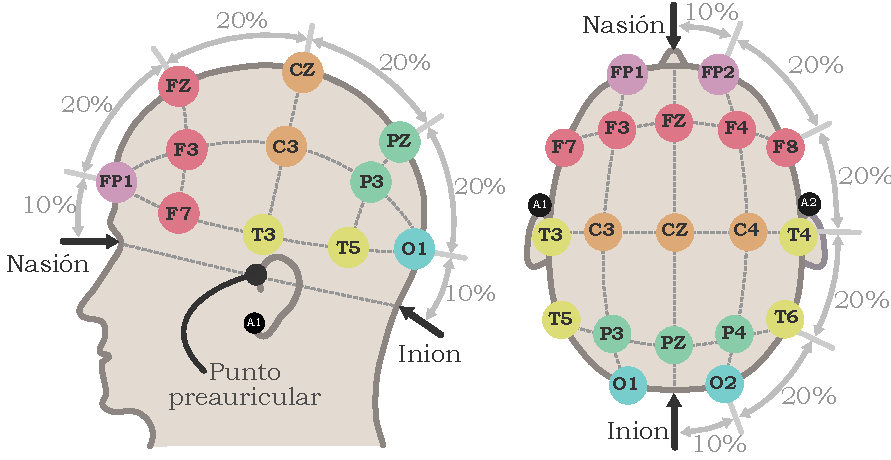
\includegraphics[width=\linewidth]{./img_diagramas/cabeza_proporcionada_color_v4.pdf} 
%\vspace{2em}
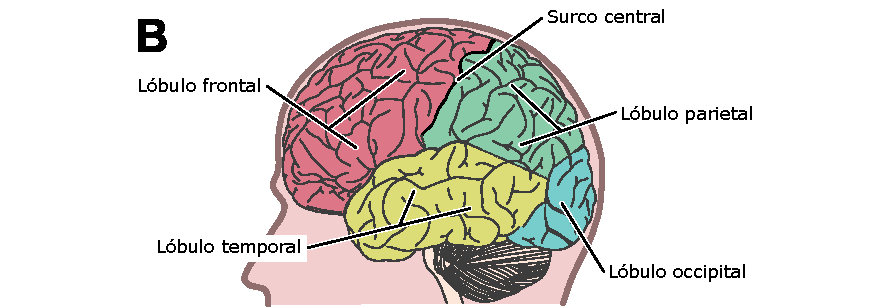
\includegraphics[width=\linewidth]{./img_diagramas/cerebro_1020_v5.pdf} 
\caption[Colocación de electrodos según el sistema 10--20]{Colocación de electrodos según el sistema 10--20. \textbf{A.} Los electrodos se colocan en una malla de longitudes relativas (medidas en porcentajes) respecto a tres puntos de referencia: inion, nasion, punto preauricular.
%; los números impares se ubican a la izquierda, los pares a la derecha y se usa la Z para el eje central. 
%En el montaje ilustrado se usan como referencia neutral a los lóbulos de las orejas, electrodos cortocircuitados A1 y A2. 
\textbf{B.} División de la corteza cerebral en lóbulos, mostrando a grosso modo qué regiones son registradas usando el EEG. Los electrodos del sistema son referidos según los lóbulos cerebrales que \textit{representan}: \underline{F}rontal, \underline{F}ronto\underline{p}olar, \underline{T}emporal, \underline{P}arietal, \underline{O}ccipital. Adicionalmente se registra cerca del surco \underline{C}entral, y los lóbulos \underline{A}uriculares; estos últimos son usados como puntos con actividad eléctrica negligible.
%\textbf{C.} Representación esquemática de los electrodos en el sistema 10--20, añadiendo los electrodos para actividad ocular y muscular. Se usarán diagramas en base a éste para reportar resultados.
}
\label{img1020}
\end{figure}

Para hablar sobre la forma en que se conectan lo electrodos entre sí, se denota a un par de electrodos como una \textbf{derivación} (también referida como \textit{canal}), mientras que el conjunto de derivaciones es un \textbf{montaje}.
%
En el contexto del presente trabajo se utilizó un montaje \textit{monopolar} (o también llamado \textit{referencial}) en cual se forman las derivaciones conectando en paralelo a cada electrodo con sus respectivos electrodos auriculares cortocircuitados y se usó como tierra a un electrodo colocado en la parte frontal media.

Es importante mencionar que las neuronas en la corteza cerebral tienen orientaciones muy diversas y que disparan de manera asíncrona, de modo que un periodo de gran actividad cerebral bien puede ser visto en el EEG como una actividad desorganizada y de baja amplitud.
%
En otra perspectiva, el cerebro se encuentra cubierto por las capas meninges, por el líquido encefalorraquídeo, el cráneo y el cuero cabelludo; en suma, los campos eléctricos generados en la corteza cerebral son \textit{víctimas} de una gran difusión espacial.
%
Es por ello que las señales captadas por los electrodos deben ser amplificadas analógicamente antes de ser registradas digitalmente.
%%
%A ello hay que añadir la difusión generada por las meninges, el líquido encefalorraquídeo y el 
%cráneo.

Un efecto colateral de amplificar la señal es la inclusión de \textbf{ruido}, entendiendo con ello a las señales que son registradas de manera no deseada.

Por ejemplo, los músculos faciales generan campos eléctricos con una frecuencia aproximada de 100 \hz; este tipo de ruidos \textit{persistentes} (referido como \textit{ruido de fondo}) son eliminados usando filtros de banda.
%
En contraparte, los ruidos esporádicos de corta duración, típicamente son señalados \textit{a mano} y provocan que el segmento de registro sea invalidado; por ejemplo, el deslizamiento de un electrodo sobre el cuero cabelludo.

%; como ejemplo, pestañear 
%voluntariamente durante un episodio de quietud mental interrumpe las ondas alfa por cerca de dos 
%segundos. 

Como comentario, cabe mencionar que el
%es posible usar electrodos colocados en otras zonas del cerebro, lo cual conlleva a técnicas similares con nombres diferentes; por ejemplo el electrocorticograma obtenido directamente de la corteza cerebral.
%
%Así mismo, se menciona que el 
término EEG suele usarse independientemente de la cantidad y posición de electrodos usados para el registro: se pueden usar sólo algunas derivaciones del sistema 10--20, se pueden hacer cambios como el uso de la nariz como referencia neutral, o se pueden añadir más electrodos como en el sistema 10--10 \cite{Klem99}. 

%%%%%%%%%%%%%%%%%%%%%%%%%%%%%%%%%%%%%%%%%%%%%%%%%%%%%%%%%%%%%%%%%%%%%%%%%%%%%%%%%%%%%%%%%%%%%%%%%%%

\subsection{Polisomnografía}
\label{sec:emg_eog}

La técnica de PSG consiste en el registro simultáneo durante el sueño de múltiples variables \textit{variables fisiológicas} como respiración, ritmo cardíaco, temperatura, entre otros.
%
La decisión sobre las señales que componen la PSG depende del problema específico que será estudiado.
%
%En el contexto del presente trabajo conviene destacar 
%
Para ayudar en la clasificación de etapas de sueño, en el contexto del presente trabajo se usó una PSG con registros de actividad ocular, tono muscular y actividad cerebral (EEG).

%En el estudio por Vázquez Tagle y colaboradores, el registro de PSG incluyó registros de actividad 
%ocular (\textbf{electrooculograma}, EOG) y tono muscular (\textbf{electromiograma}, EMG), según las 
%recomendaciones de la AASM para clasificar las etapas de sueños. La ubicación estos últimos 
%electrodos es ilustrada en la figura \ref{emg_eog}.

La actividad ocular es registrada usando la electrooculografía (EOG), una técnica que explota el comportamiento del ojo como un dipolo cuyos polos son la retina y la pupila; los movimientos del ojo inducen variaciones en el campo eléctricos generados por los electrodos de registro.
%
El registro del EOG incluye una derivación para cada ojo, LOG y ROG, conectado con el electrodo auricular cortocircuitado.
%
Así como con el EEG, la ubicación de los electrodos para EOG se indican en la figura \ref{emg_eog}.
%
%El electrodo derecho se ubica 1 cm arriba y 1 cm a la derecha del rabillo derecho de ese ojo, mientras que el izquierdo tiene una posición similar pero debajo del ojo izquierdo; para una mejor explicación ver la figura \ref{emg_eog}.
%
Cabe mencionar que el registro de EOG debe ser interpretado como el movimiento del ojo, proyectado sobre el eje formado por los electrodos de registro.

El tono muscular es vigilado usando la técnica de electromiografía (EMG), la cual \textit{observa} la actividad eléctrica producida por las fibras musculares.
%
Su registro contempla 
%una derivación diferente al resto del PSG, pues contempla 
una derivación (EMG) con tres electrodos que actúan eléctricamente como tierra, fase y neutro;
%
la ubicación de estos electrodos se indica en la figura \ref{emg_eog}. De forma parecida a esta figura, aunque en los músculos del mentón, en el presente trabajo se colocaron dos electrodos referenciados bipolarmente.  
%
En el contexto del presente trabajo, se espera observar la \textit{casi desaparición} del tono muscular para la detección del sueño MOR.
%
% el tono muscular corresponde a la contracción constante y pasiva (sin movimiento) de los músculos, siendo característica su \textit{desaparición} durante el sueño MOR.
%
%Los registros de EMG (canal EMG) admiten una interpretación más \textit{sencilla}, ya que los
%músculos son activados directamente por señales eléctricas: el tono muscular es la actividad 
%muscular basal, y se relaciona con la velocidad con que los músculos pueden \textit{salir} del 
%reposo.

A modo de comentario, en la figura \ref{ejemplos_mor} se muestra parte de un registro de PSG durante sueño MOR exhibiendo las características descritas previamente.
%, mostrando las características descritas previamente.

\begin{figure}
\centering
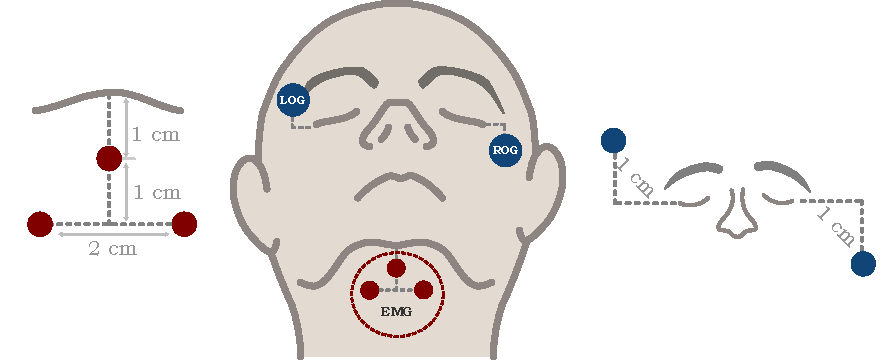
\includegraphics[width=\linewidth]
{./img_diagramas/emg_eog_v4.pdf}
\caption[Colocación de electrodos para el registro de electrooculograma y electromiograma]{Colocación de electrodos para el registro de electrooculografía en ambos ojos (LOG, ROG) y electromiografía (EMG). Las líneas punteadas son paralelas al eje medial, y las líneas discontinuas son perpendiculares al mismo. La línea de referencia para EMG inicia en el punto medial en la barbilla.}
\label{emg_eog}
\end{figure}



\begin{figure}
\centering
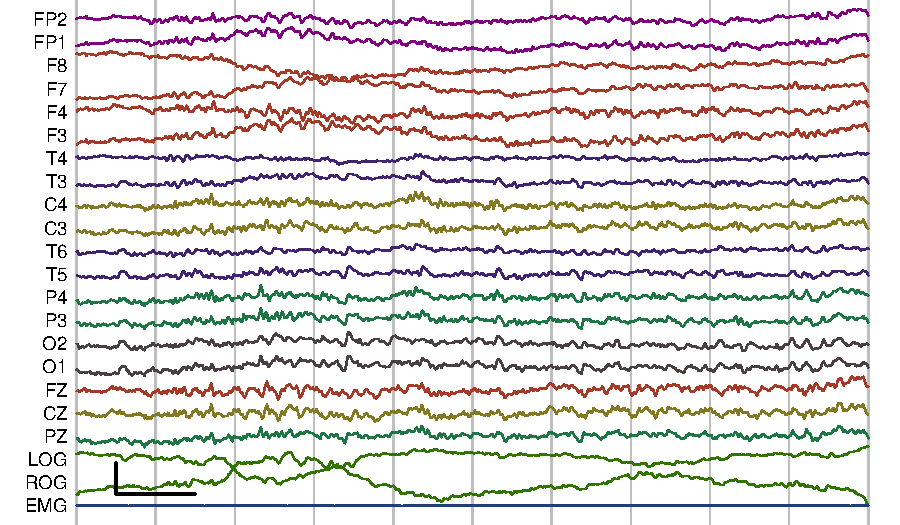
\includegraphics[width=\linewidth]
{./img_ejemplos/MJNN_epoca_stam.pdf}
\caption[Registro de polisomnograma durante sueño MOR]
{Registro de PSG durante sueño MOR. En el margen izquierdo se indica la derivación representada; aunque la mayoría corresponden al EEG, en la porción inferior se contempla al EOG y EMG.
Para más detalles sobre la ubicación de las derivaciones, ver el texto y la figura \ref{emg_eog}. Marca de calibración: vertical, 10 \mv, horizontal, 1 segundo.}
\label{ejemplos_mor}
\end{figure}

%%%%%%%%%%%%%%%%%%%%%%%%%%%%%%%%%%%%%%%%%%%%%%%%%%%%%%%%%%%%%%%%%%%%%%%%%%%%%%%%%%%%%%%%%%%%%%%%%%%
%%%%%%%%%%%%%%%%%%%%%%%%%%%%%%%%%%%%%%%%%%%%%%%%%%%%%%%%%%%%%%%%%%%%%%%%%%%%%%%%%%%%%%%%%%%%%%%%%%%

%\section{Relación entre deterioro cognitivo y sueño}
%
%Varios autores han reportado correlaciones, a nivel poblacional, entre el DCL y trastornos del sueño en adultos mayores \cite{Amer13,Miyata13,Reid06,Potvin12}.
%%
%%De forma enfática, la fase de sueño denominada MOR ha sido ampliamente relacionada con la consolidación de la memoria, así como con otras funciones cognitivas 
%%\cite{Fishbein1971,Fishbein1977,Lucero1970,Pearlman1971,Pearlman1974,Smith1991,corsi15}.
%
%El sueño MOR se ha asociado durante mucho tiempo con las funciones cognitivas \cite{Corsi1983}. 
%%
%El sueño MOR desempeña un papel en la consolidación de la memoria 
%\cite{Lucero1970, Fishbein1971, Fishbein1977, Pearlman1971, Pearlman1973, Pearlman1974, Smith1991,corsi15}.
%%
%Después de tareas complejas, hay reactivaciones de circuitos neuronales durante el sueño MOR \cite{Louie}. 
%%
%%La Potenciación a Largo Plazo (LTP) solo ocurre durante la vigilia y el sueño MOR, y, dependiendo de su fase theta del hipocampo, la LTP puede mejorarse o inhibirse \cite{Pavlides1988}.
%%
%El sueño MOR mejora la memoria y los procesos de atención mediante las entradas colinérgicas \cite{Braun1997} a través de la vía pontina \cite{Datta2004} y las estructuras del basales del cerebro anterior \cite{Blake}. 
%%
%Durante el envejecimiento normal y especialmente durante el envejecimiento patológico, los procesos de atención y memoria se vuelven más vulnerables, y las neuronas colinérgicas son las más afectadas \cite{Schliebs11}. 
%%
%%El envejecimiento afecta a varias estructuras anatómicas que resultan en la pérdida de un eje dendrítico en las neuronas corticales que muestran una degradación en su complejidad fractal estructural \cite{Lipsitz}.
%
%Se ha encontrado, por ejemplo, correlaciones entre el DCL en adultos mayores con la \textit{presencia} de ciertos tipos de ondas cerebrales \cite{babiloni13,prichep94,prichep06}.
%%
%%Sin embargo, otros estudios sugieren que el EEG durante el sueño es un mejor predictor del DCL [buscar y citar Baryet ??].
%%
%%El sueño MOR mejora la memoria y los procesos de atención mediante las entradas colinérgicas \cite{Braun} a través de pontine \cite{Datta2004} y las estructuras del basales del cerebro anterior \cite{Blake}. 
%%
%%Durante el envejecimiento normal y especialmente durante el envejecimiento patológico, los procesos de atención y memoria se vuelven más vulnerables, y las neuronas colinérgicas son las más afectadas \cite{Schliebs11}. 
%%
%%El envejecimiento afecta a varias estructuras anatómicas que resultan en la pérdida de un eje dendrítico en las neuronas corticales que muestran una degradación en su complejidad fractal estructural \cite{Lipsitz}.
%
%%Las causas inmediatas del DCL pueden rastrearse al deterioro en varias estructuras cerebrales.
%%
%Los procesos de atención y memoria dependen de circuitos colinérgicos (grupos de neuronas cuyo principal transmisor es la acetilcolina); estos circuitos son propensos a degradación estructural durante el envejecimiento, y en mayor medida si es un envejecimiento patológico \cite{Schliebs11}.
%%
%Cabe destacar que los circuitos colinérgicos son activados de forma importante durante el sueño, particularmente en la fase deniminada MOR \cite{Braun1997}.
%
%%El EEG durante el sueño MOR ha demostrado ser un indicador del DCL en adultos mayores. 
%%
%Se ha reportado una mayor potencia absoluta y relativa en frecuencias lentas para regiones laterales \cite{Brayet16} y una menor atonía muscular \cite{Chen} para adultos mayores con DCL, respecto a individuos sanos.
%
%Los estudios anteriores han incluido análisis del EEG o del EMG, pero el EOG no se ha considerado como un posible marcador del DCL. 
%%Los tres indicadores de sueño MOR aparecen generalmente en orden consecutivo. Al ingresar a esta etapa, los husos y las ondas lentas de alta amplitud están ausentes, el EEG tiene abundantes frecuencias beta y gamma \cite{SteriadeIntracortical1996,Llinas}, hay una abrupta pérdida de voltaje que ocurre en un intervalo menos de 2 segundos \cite{Rosales-Lagarde2009}, y, luego, aparcen los movimientos oculares (MOR) característicos \cite{AASM07}.
%%\cite{Aserinsky,AASM07,Rechtshaffen1968}.
%
%%En concreto se utilizarán registros de varias señales electrofisiológicas --electroencefalograma (EEG), electrooculograma (EOG) y electromiograma (EMG)--, técnica conocida como polisomnografía (PSG)\footnote{La 
%%PSG puede contener otro tipo de señales como electrocardiograma, niveles de oxígeno en la sangre, 
%%esfuerzo respiratorio, movimiento de las piernas, entre otras}, obtenidas durante 
%%etapas específicas en el sueño del paciente.
%%%ANADÏ ESTO, checar para qué figura queda, porque debe especificarse que comunmente en la PSG se registran 2 electrodos, C3 y C4, emg y ojos. Sin embargo, como el objetivo es conocer la actividad eléctrica cerebral de más regiones, se colocaron 19 electrodos en la cabeza de cada paciente, dispuestos según el sistema 10/20. ESTO DEBE ESTAR EN EL PIE DE FIGURA CORRESPONDIENTE. NO ME ACUERDO SI ESTÁ O NO, PERO FUE QUE NOS PIDIERON QUE EXPLICARAS MÁS...Y LO DE LAS OREJAS CORTOCIRCUITADAS. CITA AL MANUAL DE NIEDERMEYER

%%%%%%%%%%%%%%%%%%%%%%%%%%%%%%%%%%%%%%%%%%%%%%%%%%%%%%%%%%%%%%%%%%%%%%%%%%%%%%%%%%%%%%%%%%%%%%%%%%%
%%%%%%%%%%%%%%%%%%%%%%%%%%%%%%%%%%%%%%%%%%%%%%%%%%%%%%%%%%%%%%%%%%%%%%%%%%%%%%%%%%%%%%%%%%%%%%%%%%%

\section{Relación entre deterioro cognitivo y sueño}
\label{sec:pdcl_sueno}

Durante el envejecimiento ocurren diversos cambios fisiológicos y psicológicos que conllevan a modificaciones en el estilo de vida, y particularmente en la rutina de sueño.
%
%Es un estereotipo común que dichos cambios están íntimamente relacionados con las enfermedades no-transmisibles relacionadas con la edad
%
Hay una vasta cantidad de estudios que han explorado la posible relación entre trastornos del sueño y marcadores \textit{biológicos} de daño neuronal (como la presencia de proteína $\beta$-amiloide, marcador de la enfermedad de Alzheimer) o marcadores de actividad cerebral anómala; la tendencia es considerar que los trastornos del sueño contribuyen en el proceso de deterioro cognitivo, o bien que pueden predecirlo con cierto grado de exactitud \cite{porter15}.
%
%Pese a que son muchos los estudios que exploran la relación, 

%se han criticado los resultados obtenidos y las conclusiones obtenidas de ellos; de manera generalizada enfrentan el problema de usar grupos muestrales muy reducidos

%Cabe comentar, como experiencia personal, que el uso de grupos muestrales pequeños responde principalmente a la situación social y económica en que se encuentran los adultos mayores, especialmente ante los estereotipos asociados al deterioro cognitivo --cuando menos en el caso particular de Hidalgo.


%%%Varios autores han reportado correlaciones, a nivel poblacional, entre el DCL y trastornos del sueño en adultos mayores \cite{Amer13,Miyata13,Potvin12,Reid06}.
%Varios autores han reportado correlaciones, a nivel poblacional, entre el DCL y trastornos del sueño en adultos mayores \cite{Potvin12,Reid06}.

%Así mismo, es necesario mencionar que el presente trabajo presenta efectivamente una de las deficiencias mencionadas, ya que se ha considerado un total de 9 participantes divididos en dos grupos.
%
%Con base en lo anterior, se ha decidido enfatizar el estudio del sueño como unidad de estudio (en lugar del individuo).
%
%Adicionalmente, el estudio del

Tradicionalmente se considera que el sueño MOR desempeña un papel importante en la cognición, particularmente en la consolidación de la memoria \cite{Corsi1983}.
%
Se ha reportado que los periodos de aprendizaje inducen una mayor duración del sueño MOR y densidad de movimientos oculares rápidos, y también que la privación del sueño MOR se asocia con deficiencias en tareas de memoria \cite{smith96,smith01}.

%-------

Se ha propuesto que el mecanismo neurológico asociado a la consolidación de la memoria no es exclusivo del sueño MOR, sino que el conjunto de procesos involucrados se \textit{distribuyen} durante las diferentes etapas del sueño;
%bajo esta hipótesis, la porción del proceso ocurrida en MOR corresponde a la fijación de 
la porción del proceso ocurrida en sueño MOR corresponde a la \textit{asimilación} de información \cite{diekelmann10}.
%
%De manera más concreta, se ha sugerido que este mecanismo es \textit{inicializado} por algunas neuronas específicas en el tallo cerebral\footnote{El tallo cerebral es una porción de la médula espinal fuera de la columna vertebral, que conecta con el cerebro. En la figura \ref{img1020}.B, el tallo cerebral aparece como una estructura cilíndrica debajo del cerebro.}, referidos como vía pontina \cite{datta06}.

Anatómicamente, la consolidación de la memoria está relacionada con el sistema colinérgico\footnote{Circuitos neuronales que usan la acetilcolina como neurotransmisor principal.} en la parte anterior del cerebro 
%(lóbulos parietal y occipital) 
\cite{Blake}.
%
%En el contexto del presente trabajo este 
%%es particularmente 
%dato es muy importante
%importante, ya que los
Esto es destacable ya que los 
%Este dato es particularmente importante en el contexto del presente trabajo
circuitos colinérgicos son particularmente vulnerables a degradación estructural durante el envejecimiento y sobre todo en presencia de patologías \cite{Schliebs11}.

%xxxxx 

%El sueño MOR desempeña un papel en la consolidación de la memoria 
%%\cite{Lucero1970, Fishbein1971, Fishbein1977, Pearlman1971, Pearlman1973, Pearlman1974, Smith1991,corsi15}.
%\cite{corsi15}.
%
%Después de tareas complejas, hay reactivaciones de circuitos neuronales durante el sueño MOR \cite{Louie}. 
%
%El sueño MOR mejora la memoria y los procesos de atención mediante las entradas colinérgicas \cite{Braun1997} a través de la vía pontina \cite{Datta2004} y las estructuras del basales del cerebro anterior \cite{Blake}. 
%El sueño MOR mejora la memoria y los procesos de atención mediante las entradas colinérgicas a través de la vía pontina \cite{Datta2004} y las estructuras del basales del cerebro anterior \cite{Blake}. 

%Durante el envejecimiento normal y especialmente durante el envejecimiento patológico, los procesos de atención y memoria se vuelven más vulnerables, y las neuronas colinérgicas son las más afectadas \cite{Schliebs11}. 
%%
%Los procesos de atención y memoria dependen de circuitos colinérgicos (grupos de neuronas cuyo principal transmisor es la acetilcolina); estos circuitos son propensos a degradación estructural durante el envejecimiento, y en mayor medida si es un envejecimiento patológico \cite{Schliebs11}.



%-------------------------------------------------------------------------------
%-------------------------------------------------------------------------------
%Se ha encontrado, por ejemplo, correlaciones entre el DCL en adultos mayores con la \textit{presencia} de ciertos tipos de ondas cerebrales \cite{babiloni13,prichep94,prichep06}.
%
%Se ha reportado una mayor potencia absoluta y relativa en frecuencias lentas para regiones laterales \cite{Brayet16} y una menor atonía muscular \cite{Chen} para adultos mayores con DCL, respecto a individuos sanos.
%-------------------------------------------------------------------------------
%-------------------------------------------------------------------------------


%Cabe destacar que los circuitos colinérgicos son activados de forma importante durante el sueño, particularmente en la fase deniminada MOR \cite{Braun1997}.



%-------------
%
%Se ha encontrado, por ejemplo, correlaciones entre el DCL en adultos mayores con la \textit{presencia} de algunos tipos de ondas cerebrales \cite{babiloni13,prichep06,prichep94}.
%%
%Conviene destacar se algunos reportes sugieren que la PSG (incluso sólo el EEG durante el sueño) es un mejor predictor del DCL \cite{Brayet16}.

%%%%%%%%%%%%%%%%%%%%%%%%%%%%%%%%%%%%%%%%%%%%%%%%%%%%%%%%%%%%%%%%%%%%%%%%%%%%%%%%%%%%%%%%%%%%%%%%%%%
%%%%%%%%%%%%%%%%%%%%%%%%%%%%%%%%%%%%%%%%%%%%%%%%%%%%%%%%%%%%%%%%%%%%%%%%%%%%%%%%%%%%%%%%%%%%%%%%%%%
%%%%%%%%%%%%%%%%%%%%%%%%%%%%%%%%%%%%%%%%%%%%%%%%%%%%%%%%%%%%%%%%%%%%%%%%%%%%%%%%%%%%%%%%%%%%%%%%%%%
%%%%%%%%%%%%%%%%%%%%%%%%%%%%%%%%%%%%%%%%%%%%%%%%%%%%%%%%%%%%%%%%%%%%%%%%%%%%%%%%%%%%%%%%%%%%%%%%%%%

%%%%%%%%%%%%%%%%%%%%%%%%%%%%%%%%%%%%%%%%%%%%%%%%%%%%%%%%%%%%%%%%%%%%%%%%%%%%%%%%%%%%%%%%%%%%%%%%%%%
%%%%%%%%%%%%%%%%%%%%%%%%%%%%%%%%%%%%%%%%%%%%%%%%%%%%%%%%%%%%%%%%%%%%%%%%%%%%%%%%%%%%%%%%%%%%%%%%%%%
%%%%%%%%%%%%%%%%%%%%%%%%%%%%%%%%%%%%%%%%%%%%%%%%%%%%%%%%%%%%%%%%%%%%%%%%%%%%%%%%%%%%%%%%%%%%%%%%%%%
%%%%%%%%%%%%%%%%%%%%%%%%%%%%%%%%%%%%%%%%%%%%%%%%%%%%%%%%%%%%%%%%%%%%%%%%%%%%%%%%%%%%%%%%%%%%%%%%%%%

\chapter{Metodología y resultados}
\label{ch:metodologia}

El presente trabajo surge a partir de una colaboración con el Laboratorio de Sueño, Emoción y Cognición, del Instituto de Ciencias de la Salud de la UAEH a cargo de la Dra. Alejandra Rosales Lagarde.
%
Esta colaboración permitió el acceso a los registros obtenidos en un estudio comenzado por la Dra. Rosales y por Vázquez-Tagle durante los años de 2014 a 2017 \cite{VazquezTagle16}. 
%
Dicha investigación se centró en el estudio del deterioro cognitivo en adultos mayores del estado de Hidalgo, y consideró registros de PSG para evaluar parámetros relacionados al sueño y en especial al sueño MOR.
%
El presente trabajo tiene como objetivo particular analizar con mayor detalle dichos registros.

En este capítulo se describe primeramente la metodología seguida para obtener los registros de PSG.
%
Posteriormente se describe la metodología usada para analizar los registros de PSG, usando las herramientas descritas en el capítulo \ref{capitulo:espectro_evo}.

Los registros de PSG fueron segmentados en ventanas de 30 segundos, referidas como \textbf{épocas}.
%
El análisis de los registros de PSG se llevó a cabo a tres niveles:
\begin{itemize}
\item Dentro de cada época.
\item Entre las diferentes épocas en un registro.
\item Entre los diferentes participantes.
\end{itemize}

El análisis a nivel de época contempla su clasificación según etapa de sueño (limitada a MOR y NMOR), y su clasificación como estacionarias o no estacionarias (usando la prueba de PSR).
%
El uso de épocas como unidades de estudio se justifica por la gran heterogeneidad del sueño nocturno; paralelamente, destaca el supuesto fisiológico de que las etapas de sueño son \textit{parecidas} entre los humanos.
%
En suma, los registros de PSG para un sólo individuo pueden interpretarse como una población de épocas.

El análisis a nivel de registro surge de considerar la heterogeneidad del sueño pero usando al registro entero como unidad de estudio.
%
El tomar las épocas junto con su estructura temporal reveló algunos patrones interesantes de actividad.

Para el análisis entre participantes (divididos en grupos), varias de las características descritas fueron \textit{colapsadas} para constituir características \textit{simples}. 
%
Debido a las características de la muestra (ver más adelante), los resultados obtenidos no pueden extrapolarse a la población en general.
%
Los resultados obtenidos, entonces, se presentan como \textit{indicios}.

%Cabe mencionar que, por mera precaución, 
Los resultados en los tres tipos de análisis fueron repetidos usando la clasificación de estacionariedad obtenida para diferentes tamaños de ventana.
%
Bajo el supuesto de estacionariedad local es, en principio, posible que la estimación de varias características se vea afectada por el tamaño de ventana utilizado; este efecto es cualitativamente diferente que el de la cantidad de puntos considerados.
%
Para mayor información sobre el efecto esperado por la estacionariedad local, ver sección \ref{sec:est_local}.

%%%%%%%%%%%%%%%%%%%%%%%%%%%%%%%%%%%%%%%%%%%%%%%%%%%%%%%%%%%%%%%%%%%%%%%%%%%%%%%%%%%%%%%%%%%%%%%%%%%

\section{Características de los participantes}

Los participantes fueron elegidos usando un muestreo \textit{no probabilístico por conveniencia} bajo los siguientes criterios de inclusión:
\begin{itemize}
\item Edad entre 60 y 85 años.
\item Diestros (mano derecha dominante).
\item Sin ansiedad, depresión ni síndromes focales.
\item No usar medicamentos o sustancias para dormir.
\item Firma de consentimiento informado.
\item Terminar el estudio de forma voluntaria en lo que corresponde a la aplicación de pruebas y el registro de la PSG.
\end{itemize}

Un total de 16 adultos mayores cumplieron los criterios de inclusión. 
%
Con el fin de detectar el DCL en estos pacientes, éstos fueron sometidos a una batería de pruebas neuropsicológicas para determinar su estado cognoscitivo general (Neuropsi, MMSE), detectar cambios en su vida cotidiana (KATZ) y descartar cuadros ansiosos y depresivos (SAST, GDS); para más detalles ver capítulo anterior, sección \ref{seccion:pruebas}.
%
En la tabla \ref{tab_sujetos} se reportan los puntajes obtenidos por los participantes en dichas pruebas; estos datos deben ser interpretados según los \textit{puntajes de corte} de cada prueba, que se incluyen en el apéndice \ref{apendice_pruebas}.
%reportados en las tablas \refrange{anexo:sast_gds,anexo:mmse,anexo:neuropsi,anexo:katz}.
% \crefrange{anexo:sast_gds,anexo:mmse,anexo:neuropsi,anexo:katz}.
%
Se determinó que 11 de los voluntarios no padecen depresión o ansiedad, ni presentan afectaciones significativas en la vida diaria; el participante MGG presenta un cuadro depresivo, pero fue incluido en ausencia de afecciones cognitivas objetivas y porque el sueño presentó una arquitectura de sueño normal, de acuerdo a una experta en neurofisiología quien analizó todos los registros. Cabe señalar que los pacientes con depresión suelen tener una latencia al sueño MOR más corta y en esta paciente fue normal.
%
Debido a motivos técnicos, sólo 9 participantes fueron considerados para el presente trabajo; se reportan únicamente los datos relativos a esos participantes.

Con base en el diagnóstico de PDCL, los 9 participantes fueron divididos en dos grupos: PDCL y CTRL. 
%
Es importante mencionar que, bajo las condiciones muestrales, el grupo CTRL no puede fungir satisfactoriamente como grupo control; una descripción más adecuada sería \textit{grupo sin PDCL}.

%Para esta clasificación se dio mayor atención al puntaje de Neuropsi, estandarizado según edad y 
%escolaridad (cuadro \ref{puntajes}). 
%
%Cabe mencionar que intencionalmente se dio menor importancia a los puntajes de la prueba MMSE en cuanto al diagnóstico del PDCL; ésto porque se ha reportado que, en la población mexicana, esa prueba tiene baja sensibilidad para el diagnóstico de DCL en general, y baja especificidad para individuos con escolaridad muy baja o muy alta \cite{Ostrosky00}.
%%
%Para fines del comentario anterior, se entiende por \textit{sensibilidad} a la probabilidad de obtener verdaderos positivos, y por \textit{especificidad} a la probabilidad de obtener verdaderos negativos.

\begin{table}
\caption{Datos generales de los participantes}
\centering
\bordes{1.1}
{\small
\begin{tabular}{llcrrrrrrr}
\toprule
 \phantom{mmm}&
 & {Sexo} & {Edad} & {Escol.} & {Neuropsi} & {MMSE} & {SAST} & {KATZ} & {GDS} \\
\midrule
\multicolumn{2}{l}{\textbf{Grupo CTRL}}\\
&MJH    & F    & 72\pz & 9\pz  & 113\pz & 30\pz & 18\pz & 0\pz & 0\pz  \\
&JAE    & F    & 78\pz & 5\pz  & 102\pz & 28\pz & 19\pz & 0\pz & 5\pz  \\
&MGG    & F    & 61\pz & 9\pz  & 114\pz & 28\pz & 29\pz & 1\pz & 14\pz \\
&EMT    & F    & 50\pz & 22\pz & 117\pz & 30\pz & 15\pz & 0\pz & 4\pz  \\
\rowcolor{gris}
&\multicolumn{1}{c}{$\widehat{\mu}$} & 
               & 65.3  & 11.3  & 111.5  & 29.0  & 20.3  & 0.3  & 5.8  \\
\rowcolor{gris}
&\multicolumn{1}{c}{$\widehat{\sigma}$} & 
               & 12.4  & 7.4   & 6.6    & 1.2   & 6.1   & 0.5  & 5.9  \\
\midrulec
%\hline
\multicolumn{2}{l}{\textbf{Grupo PDCL}}\\
& CLO   & F    & 68\pz &  5\pz &  81\pz & 28\pz & 22\pz & 1\pz &  6\pz \\
& RLO   & F    & 63\pz &  9\pz &  90\pz & 29\pz & 20\pz & 0\pz &  3\pz \\
& JGZ   & M    & 65\pz & 11\pz &  87\pz & 25\pz & 20\pz & 0\pz &  1\pz \\
& AEFP  & M    & 73\pz &  8\pz &  96\pz & 29\pz &   \pz & 0\pz &  2\pz \\
& PCM   & M    & 71\pz &  9\pz & 111\pz & 28\pz & 20\pz & 0\pz & 10\pz \\
\rowcolor{gris}
&\multicolumn{1}{c}{$\widehat{\mu}$} & 
              &  68.0  & 8.4   & 93.0   & 27.8  & 20.5  & 0.2  & 4.4  \\
\rowcolor{gris}
&\multicolumn{1}{c}{$\widehat{\sigma}$} & 
              & 4.1    & 2.2   & 11.4   & 1.6   & 1.0   & 0.4  & 3.6 \\
\bottomrulec
\end{tabular} 
}
\label{tab_sujetos}
\end{table}

%%%%%%%%%%%%%%%%%%%%%%%%%%%%%%%%%%%%%%%%%%%%%%%%%%%%%%%%%%%%%%%%%%%%%%%%%%%%%%%%%%%%%%%%%%%%%%%%%%%
%%%%%%%%%%%%%%%%%%%%%%%%%%%%%%%%%%%%%%%%%%%%%%%%%%%%%%%%%%%%%%%%%%%%%%%%%%%%%%%%%%%%%%%%%%%%%%%%%%%

\subsection{Registro del polisomnograma}

Para efectuar el registro de la PSG, los participantes acudieron a las instalaciones del Laboratorio de Sueño, Emoción y Cognición. 
%
Los participantes recibieron instrucciones de realizar una rutina normal de actividades durante la semana que precedió al estudio, y se les recomendó no ingerir bebidas alcohólicas o energizantes (como café o refresco) durante las 24 horas previas al experimento, y que no durmieran siesta ese día.
%
Bajo estas condiciones experimentales se garantiza que los registros son representativos del sueño nocturno de cada participante.

El registro per se fue efectuado usando un polisomnógrafo Medicid 5 (Neuronic Mexicana). El montaje de la PSG incluyó los siguientes electrodos\footnote{Para más detalles ver el capítulo anterior, particularmente la sección \ref{capitulo:psg}}:
\begin{itemize}
\item 19 electrodos de EEG colocadas según el Sistema Internacional 10--20.
\item 2 electrodos de EOG para movimientos oculares.
\item 2 electrodos de EMG para medir el tono muscular en los músculos del mentón.
\end{itemize}

Los electrodos para EEG fueron conectados en paralelo usando como referencias los lóbulos de las orejas cortocircuitadas; la impedancia se mantuvo por debajo de \SI{50}{\micro\ohm}.
%
Las señales fueron amplificadas analógicamente usando amplificadores de alta ganancia en cadena, 
y adicionalmente fueron \textit{pasado} filtros analógicos pasa bandas: 0.1--100 Hz 
para EEG, 3--20 Hz para EOG. 
%
Los registros fueron digitalizados con una frecuencia de muestreo de 512 puntos por segundos (Hz), y posteriormente almacenados en formato de texto.

Como se mencionó anteriormente, los registros fueron segmentados en segmentos de 30 segundos, referidas como \textbf{épocas}; en lo posterior se usará la palabra `época' como un caso particular de la ventana.
%
Cada una de las épocas fue clasificada como MOR o NMOR; la clasificación fue llevada a cabo por dos expertos de ICSA y una neurofisióloga de la UNAM, y bajo los estándares de la AASM.

Por simplicidad técnica, los registros fueron truncados para poder considerar épocas completas; algunos datos al final de cada registro fueron omitidos, aunque representan una cantidad negligible de tiempo.
%
Cabe mencionar que cada época de 30 segundos, a una frecuencia de 512 Hz, representa un total de 15,360 puntos.

En la tabla \ref{tab:psg} se describe la duración de los registros, así como la cantidad de tiempo del registro clasificado como sueño MOR.
%
La cantidad de tiempo en vigilia registrado es negligible ($<5$ minutos por cada participante), de modo que ésta no es reportada; con una pérdida mínima de generalidad, se puede afirmar que los registros fuera del sueño MOR corresponden a sueño NMOR.

\begin{table}
\centering
\caption{Datos generales sobre los registros de PSG}
\bordes{1.2}
\begin{tabular}{lllrclrr}
\toprule
    \phantom{mmm}&
    & \multicolumn{2}{l}{TTS} & \phantom{l}   & \multicolumn{3}{l}{MOR*}\\
    \cmidrule{3-4}  \cmidrule{6-8}
    &          &Épocas  &  Min.   &&Épocas  &  Min.   &  \% \\
\midrule
\multicolumn{2}{l}{\textbf{Grupo CTL}}\\
&MJH &    1032   &  516\pz && 127    & 63.5  &12.31 \\
&JAE &\ppu 904   &  452\pz && 171    & 85.5  &18.92 \\
&MGG &    1024   &  512\pz && 166    & 83\pz &16.21 \\
&EMT &\ppu 552   &  276\pz &&  47    & 23.5  & 8.51 \\
 
\rowcolor{gris}
&\multicolumn{1}{c}{$\widehat{\mu}$}  
     &\ppu 878.0 &  439.0  && 128.0  & 63.9  &13.99 \\
\rowcolor{gris}
&\multicolumn{1}{c}{$\widehat{\sigma}$} 
     &\ppu 225.1 &  112.5  &&  57.3  & 28.7  &4.55 \\ 
\midrulec

\multicolumn{2}{l}{\textbf{Grupo PDC}}\\
&CLO  &\ppu 944   & 472\pz && 132\pz & 66\pz & 13.98 \\
&RLO  &\ppu 840   & 420\pz &&  99\pz & 49.5  & 11.79 \\
&JGZ  &    1200   & 600\pz &&  34\pz & 17\pz &  2.83 \\
&AEFP &\ppu 952   & 476\pz &&  41\pz & 20.5  &  4.31 \\
&PCM  &\ppu 752   & 376\pz &&  59\pz & 29.5  &  7.85 \\
 
\rowcolor{gris}
&\multicolumn{1}{c}{$\widehat{\mu}$}  
      &\ppu 937.6 & 468.8 &&   73.0  & 36.5  & 8.15 \\
\rowcolor{gris}
&\multicolumn{1}{c}{$\widehat{\sigma}$} 
      &\ppu 168.1 &  84.1 &&   41.5  & 20.8  & 4.75 \\
\bottomrulec
%\multicolumn{8}{l}{*El sueño MOR aparece fragmentado, se reporta la suma de tales tiempos.}\\
%\multicolumn{8}{l}{TTS= Tiempo Total de sueño.}\\
\end{tabular} \\
\begin{small}
\begin{tabular}{l}
{*El sueño MOR aparece fragmentado, se reporta la suma de tales tiempos.}\\
{TTS= Tiempo Total de sueño.} {El porcentaje de sueño MOR se calcula respecto al TTS.}
\end{tabular}
\end{small}
\label{tab:psg}
\end{table}

%%%%%%%%%%%%%%%%%%%%%%%%%%%%%%%%%%%%%%%%%%%%%%%%%%%%%%%%%%%%%%%%%%%%%%%%%%%%%%%%%%%%%%%%%%%%%%%%%%%
%%%%%%%%%%%%%%%%%%%%%%%%%%%%%%%%%%%%%%%%%%%%%%%%%%%%%%%%%%%%%%%%%%%%%%%%%%%%%%%%%%%%%%%%%%%%%%%%%%%

\section{Características muestrales}

Previo a los análisis de los registros de PSG, se corroboró si los dos grupos de participantes efectivamente se \textit{comportan} como grupos estadísticamente diferentes.
%
Con dicho objetivo, se aplicaron pruebas $U$ de Wilcoxon-Mann-Whithney (WMW) entre los dos grupos, para todas las variables consideradas. 
%
De lo anterior se exceptúa al puntaje de la prueba KATZ, ya que es un parámetro cualitativo. 
%
Se concluye que las mediciones son parecidas en ambos grupos para todas las variables observadas, excepto para el puntaje en la prueba Neuropsi; ello era de esperarse ya que el puntaje en Neuropsi fue usado para designar a los participantes en los grupos.
%
Los resultados de estas pruebas se reportan en la tabla \ref{tab:var_wilcox}.

\begin{table}
\centering
\caption{Variables independientes entre grupos}
\begin{tabular}{lrlcrlccr}
\toprule
 & \multicolumn{2}{l}{Grupo CTRL} & \phantom{.} & \multicolumn{2}{l}{Grupo PDCL} 
 & \phantom{.} & \multicolumn{2}{l}{WMW}
 \\
\cmidrule{2-3} \cmidrule{5-6} \cmidrule{8-9}
            & Media & (DE)  & & Media & (DE) & & $p$ & $W$ \\
\midrule
Edad        &  65.3 &  12.4 & &  68.0 &  4.1 & &    0.905 &  9.0  \\
Escolaridad &  11.3 &   7.4 & &   8.4 &  2.2 & &    0.797 & 11.5 \\
Neuropsi    & 111.5 &   6.6 & &  93.0 & 11.4 & &\bf 0.032 & 19.0 \\
MMSE        &  29.0 &   1.2 & &  27.8 &  1.6 & &    0.366 & 14.0 \\
SATS        &  20.3 &   6.1 & &  20.5 &  1.0 & &    0.301 &  4.0  \\
GDS         &   5.8 &   5.9 & &   4.4 &  3.6 & &    0.905 & 11.0 \\
TTS [min]   & 439.0 & 112.5 & & 468.8 & 84.2 & &    1.000 & 10.0 \\
MOR [min]   &  63.9 &  28.7 & &  36.5 & 20.8 & &    0.190 & 16.0 \\
MOR [\%]    &  14.0 &   4.5 & &   8.2 &  4.8 & &    0.111 & 17.0 \\
\bottomrule 
\multicolumn{9}{l}{WMW=Prueba de Wilcoxon--Mann--Whitney, DE=Desviación}\\
\multicolumn{9}{l}{Estándar, TTS=Tiempo Total de Sueño.}
\end{tabular} 
\label{tab:var_wilcox}
\end{table}

Se verificó si hay correlaciones entre las variables consideradas, lo cual podría afectar la interpretación de los resultados posteriores.
%
Para ello se aplicó la prueba de correlación de Spearman a cada par de variables; la prueba de Spearman estima la correlación entre variables, y se prueba la hipótesis de que la correlación es diferente de cero.
%
Estos resultados se reportan en el cuadro \ref{tab:correlacion}.

\begin{table}
\centering
\caption{Prueba de correlación de Spearman (estimación y p-valor)}
\begin{tabular}{lcccccccc}
\toprule
             & \rotatebox{80}{Escolaridad} & \rotatebox{80}{Neuropsi} & \rotatebox{80}{MMSE} & \rotatebox{80}{SAST} & \rotatebox{80}{GDS} & \rotatebox{80}{Sueño [min]} & \rotatebox{80}{MOR [min]} & \rotatebox{80}{MOR [\%]} \\
\midrule
Edad        & -0.699 & -0.267 & -0.079 & -0.171 & -0.233 & 0.200  & 0.183  & 0.100   \\
            & (\textbf{0.04}) & (0.49) & (0.84) & (0.69) & (0.55) & (0.61) & (0.64) & (0.81)  \\
\rowcolor{gris}
Escol.      &        & 0.437  & 0.194  & -0.366 & -0.254 & -0.044 & -0.586 & -0.525  \\
\rowcolor{gris}
            &        & (0.24) & (0.62) & (0.37) & (0.51) & (0.91) & (0.10) & (0.15)  \\

Neuropsi    &        &        & 0.501  & -0.415 & 0.200  & -0.267 & 0.150  & 0.200   \\
            &        &        & (0.17) & (0.31) & (0.61) & (0.49) & (0.71) & (0.61)  \\

\rowcolor{gris}
MMSE        &        &        &        & -0.628 & -0.378 & -0.316 & -0.070 & 0.018   \\
\rowcolor{gris}
            &        &        &        & (0.09) & (0.32) & (0.41) & (0.86) & (0.96)  \\

SATS        &        &        &        &        & 0.610  & 0.317  & 0.293  & 0.195   \\
            &        &        &        &        & (0.11) & (0.44) & (0.48) & (0.64)  \\

\rowcolor{gris}
GDS         &        &        &        &        &        & -0.433 & 0.517  & 0.467   \\
\rowcolor{gris}
            &        &        &        &        &        & (0.25) & (0.16) & (0.21)  \\

Sueño [min] &        &        &        &        &        &        & -0.050 & -0.067  \\
            &        &        &        &        &        &        & (0.91) & (0.88)  \\

\rowcolor{gris}
MOR [min]   &        &        &        &        &        &        &        & 0.983   \\
\rowcolor{gris}
            &        &        &        &        &        &        &        & (\textbf{0.00})  \\
%\bottomrule
\bottomrulec
%\multicolumn{7}{l}{Niveles de significancia: *$<$.05 , **$<$.01 , ***$<$.005 , ****$<$.001}
\end{tabular}
\label{tab:correlacion}
\end{table}

Sólo se encontraron correlaciones significativas entre dos pares de variables: edad y escolaridad, y tiempo en MOR \textit{medido} en segundos y en porcentaje.

La primera relación, no muy fuerte, puede explicarse como un \textit{efecto generacional}: la educación superior ha aumentado su cobertura durante las últimas décadas, y entonces los grupos poblacionales más jóvenes tienen en promedio más años de escolaridad. 
%
%En base a estudios horizontales de larga escala, algunos autores han sugerido que un bajo nivel de escolaridad es un factor de riesgo para padecer deterioro cognitivo \cite{Mejia_Arango2007}.
%
Una segunda hipótesis para esta correlación es la contribución del participante EMT, quien tiene una edad menor y un nivel de educación mayor al resto de los participantes.
%
Para contrastar la segunda hipótesis se calculó nuevamente la prueba de Spearman pero retirando los datos de EMT: se halló una correlación estimada de 0.179 con un p-valor asociado de 0.672, que no permite rechazar el que la correlación sea diferente de cero.

Se descarta entonces la hipótesis del efecto generacional, cuando menos para el grupo de participantes considerados, y se acepta que la correlación es debida a valores atípicos. Se concluye que, usando los datos recabados, no se puede obtener información relevante sobre el efecto del nivel de educación ni la edad sobre el PDCL, ni con los marcadores del PSG que se describirán más adelante.

Intuitivamente era de esperarse la correlación entre el tiempo en MOR y el porcentaje de sueño que es MOR.
%
Sin embargo, la hipótesis de que el sueño tenga una \textit{estructura característica} --y por tanto, que las etapas de sueño aparezcan en proporciones similares en varios individuos--- es ajena a los supuestos estadísticos.
%
Con base a este resultado, en adelante se usará el porcentaje de MOR como \textit{sustituto} del tiempo real de MOR porque (1) dichas variables están fuertemente correlacionadas, y (2) porque el porcentaje permite comparar intuitivamente características de registros con duraciones muy diferentes.

%%%%%%%%%%%%%%%%%%%%%%%%%%%%%%%%%%%%%%%%%%%%%%%%%%%%%%%%%%%%%%%%%%%%%%%%%%%%%%%%%%%%%%%%%%%%%%%%%%%
%%%%%%%%%%%%%%%%%%%%%%%%%%%%%%%%%%%%%%%%%%%%%%%%%%%%%%%%%%%%%%%%%%%%%%%%%%%%%%%%%%%%%%%%%%%%%%%%%%%

\section{Análisis a nivel de época}
\label{sec:analisis_epoca}

Como se mencionó anteriormente, los registros fueron fragmentados en ventanas de 30 segundos, referidas como épocas, para su clasificación en las etapas de sueño.
%
De manera independiente, cada una de estas épocas fue sometida a la prueba de estacionariedad de Priestley--Subba Rao (PSR) para investigar si es estacionaria en el sentido de homogeneidad espectral; para más detalles ver la sección \ref{sec:psr}.

Con base en la prueba de PSR, cada una de las épocas consideradas fue clasificada como \textit{estacionaria} 
si fue rechazada la hipótesis de no--estacionariedad con un nivel de significancia $p<0.05$.
%
La aplicación per se de la prueba de PSR fue efectuada usando el software estadístico R; en particular, se utilizó la implementación incluida en el paquete \texttt{fractal} bajo la función \texttt{stationarity} \cite{R_fractal}.

Con cada época clasificada según etapa de sueño (MOR o NMOR) y según estacionariedad, se procedió primeramente a revisar cómo están relacionadas ambas características.
%
Para ello se planteó la hipótesis de que la cantidad de épocas estacionarias es diferente en MOR y NMOR. 

Debido a que la cantidad de épocas en NMOR es considerablemente mayor a las épocas en MOR, y con base en las observaciones de la sección anterior, se usaron proporciones en lugar del total de épocas.
%
Para simplificar la notación, las proporciones de épocas clasificadas como estacionarias en MOR y NMOR serán referidas como $\text{p}_{\text{MOR}}$ y $\text{p}_{\text{NMOR}}$, respectivamente; es decir
\begin{equation}
\text{p}_{\text{MOR}} = \frac{\text{\# épocas estacionarias en MOR}}{\text{\# épocas en MOR}}
\end{equation}
y similarmente para $\text{p}_{\text{NMOR}}$.
%
Dado que las clasificaciones según etapa de sueño (MOR/NMOR) y estacionariedad (sí/no) son dicotómicas, la hipótesis $\text{p}_{\text{MOR}}\neq\text{p}_{\text{NMOR}}$ fue probada usando la prueba $\chi^{2}$ de Pearson; dicha prueba fue repetida para todas las derivaciones consideradas.

Los resultados obtenidos se reportan en el apéndice \ref{apendiceA}, y en la figura \ref{cabeza_new} se muestra de forma esquemática en qué derivaciones se encontraron diferencias significativas.
%
%No se encontraron patrones claros que pudieran relacionar el PDCL --ni otros factores considerados-- con las regiones con diferencias significativas.

\begin{figure}
\centering
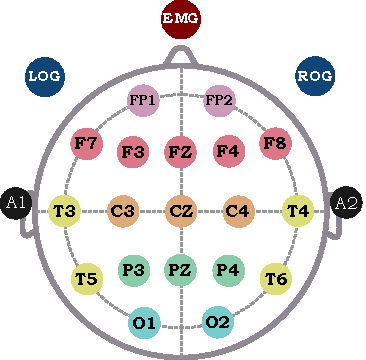
\includegraphics[scale=1.2]
{./img_diagramas/estampa_v1.pdf}
\caption{Representación minimalista de los electrodos considerados en el registro de PSG;
%: 19 para el EEG, dos para el EOG, un grupo de 3 para el EMG y dos electrodos de referencia.
para más detalles ver las secciones \ref{sec:eeg} y \ref{sec:emg_eog}.
Esta forma de ordenar las gráficas será usada en gráficos posteriores.}
\label{img:estampa}
\end{figure}

\begin{figure}
\centering
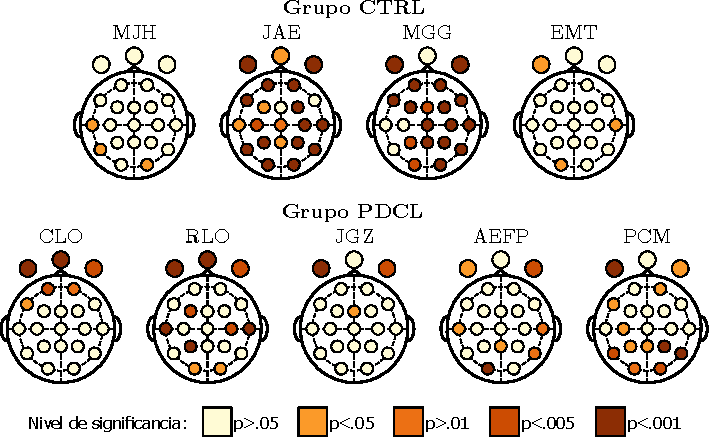
\includegraphics[width=\textwidth]{./img_art_dfa/prop_tabla.pdf} \\
\caption{Derivaciones para las cuales la proporción de épocas clasificadas como estacionarias fue significativamente diferente en MOR y NMOR.
%
En la parte superior se representa al grupo CTRL y en la parte inferior al grupo PDCL.
%
Para esta figura se usaron épocas de 30 segundos de duración.
%
La posición de los círculos representa a las derivaciones, en correspondencia con la figura \ref{img:estampa}.}
\label{cabeza_new}
\end{figure}

\subsection*{Efecto de la estacionariedad local}

%Con base en la hipótesis sobre estacionariedad local, discutida en la sección \ref{sec:est_local}, 
Se procedió a repetir la clasificación de estacionariedad pero usando ventanas de diferentes tamaños.
%
Los tamaños de ventana se eligieron de la forma $30 \times 2^{n}$ segundos por \textit{compatibilidad}, ya que el protocolo de la AASM sugiere usar épocas de 30 segundos para identificar el sueño MOR) y por motivos técnicos.
%
El tamaño de ventana más pequeño fue de $\nicefrac{30}{32}$ segundos para poder utilizar la prueba de PSR de forma confiable, mientras que el tamaño más grande fue de $120$ segundos tomando en cuenta que ventanas más grandes serían demasiado heterogéneas para considerarse como unidades de estudio fiables.

En la figura \ref{cabeza_repoio} se muestran únicamente las proporciones estimadas de épocas estacionarias para MOR y NMOR ($\text{p}_{\text{MOR}}$ y $\text{p}_{\text{NMOR}}$) para un participante; los gráficos construidos para todos los participantes pueden encontrarse en el apéndice \ref{apendiceA}.
%
Usando épocas de mayor duración, se encuentra que una proporción menor de éstas son clasificadas como estacionarias; sin embargo, usar épocas de menor duración no garantiza el efecto contrario.
%
Dicho fenómeno \textit{apoya} la hipótesis de estacionariedad local en los registros de PSG en adultos mayores, aunque no representa evidencia suficiente para relacionarlo con el PDCL.

\begin{figure}
\centering
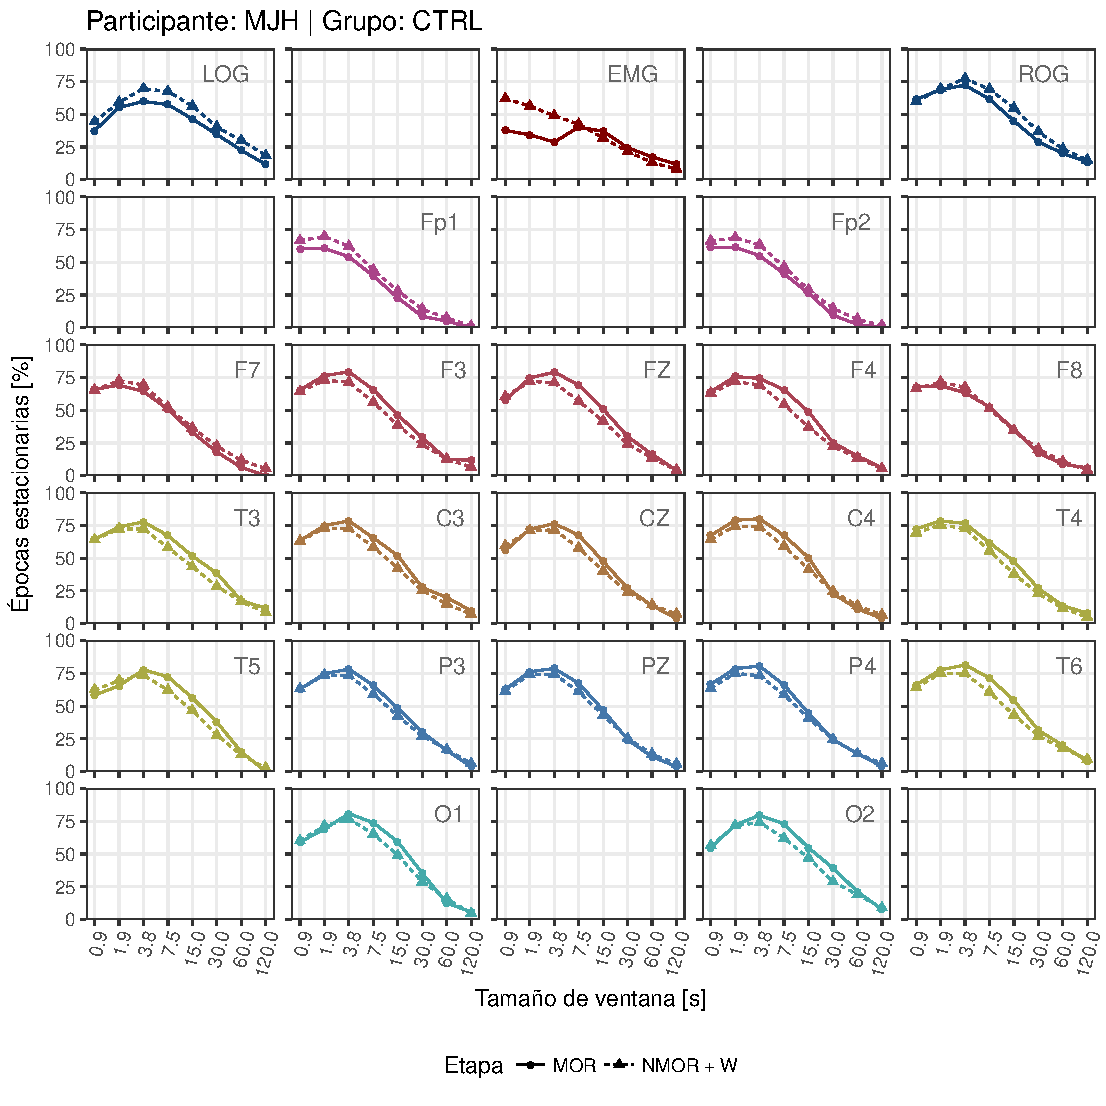
\includegraphics[width=\linewidth]{./scripts_graf_res/MJNNVIGILOS_cabeza_epocas_v2.pdf}
\caption{Cambio en la proporción de épocas estacionarias respecto al tamaño de ventana usado, durante MOR y NMOR. El análisis se repite en todas las derivaciones consideradas; la posición y color de cada gráfico se corresponden a aquellos de la figura \ref{img:estampa}. W = vigilia, recordando que la cantidad tiempo de los registros clasificada como vigilia es negligible.}
\label{cabeza_repoio}
\end{figure}

En resumen, no se pudo identificar una conexión clara entre el PDCL y las características de las épocas como unidades autónomas.
%
Debido a ello se consideran otros niveles de organización sobre los registros: los registros como un conjunto de épocas distribuidas en el tiempo con \textit{cierta estructura}, y al individuo como unidad en la variabilidad de dichas estructuras.
%
En particular sobre el último, si se supone que las cantidades descritas en esta sección son características \textit{representativas} de cada participante, entonces tiene sentido intentar verificar similitudes con otros participantes o correlaciones con otras observaciones.

%%%%%%%%%%%%%%%%%%%%%%%%%%%%%%%%%%%%%%%%%%%%%%%%%%%%%%%%%%%%%%%%%%%%%%%%%%%%%%%%%%%%%%%%%%%%%%%%%%%
%%%%%%%%%%%%%%%%%%%%%%%%%%%%%%%%%%%%%%%%%%%%%%%%%%%%%%%%%%%%%%%%%%%%%%%%%%%%%%%%%%%%%%%%%%%%%%%%%%%

\section{Análisis a nivel de registro}
\label{sec:analisis_registro}

%Como se mencionó en la sección \ref{sec:pdcl_sueno}, se han reportado cambios en la estructura del sueño en adultos mayores con deterioro cognitivo, respecto a adultos mayores saludables.
%%
%El objetivo de esta subsección es intentar detectar estos \textit{cambios de estructura} usando los métodos descritos y bajo las condiciones descritas.

Con el fin de explorar cómo se relacionan las épocas estacionarias con la \textit{estructura del sueño}, se procedió a \textit{graficar} la estacionariedad.
%
Para efectuar lo anterior se consideró una cuadrícula, con una fila por cada derivación y una columna por cada época analizada (se registró el mismo número de épocas para cada derivación); sobre la cuadrícula el espacio correspondiente a cada época fue coloreado a según la clasificación de la época como estacionaria.
%
Se procedió similarmente para ilustrar la clasificación según etapa de sueño.
%
En la figura \ref{img:patrones} se ejemplifica este tipo de gráficos, además de otros detalles a mencionarse.

\begin{figure}
\centering
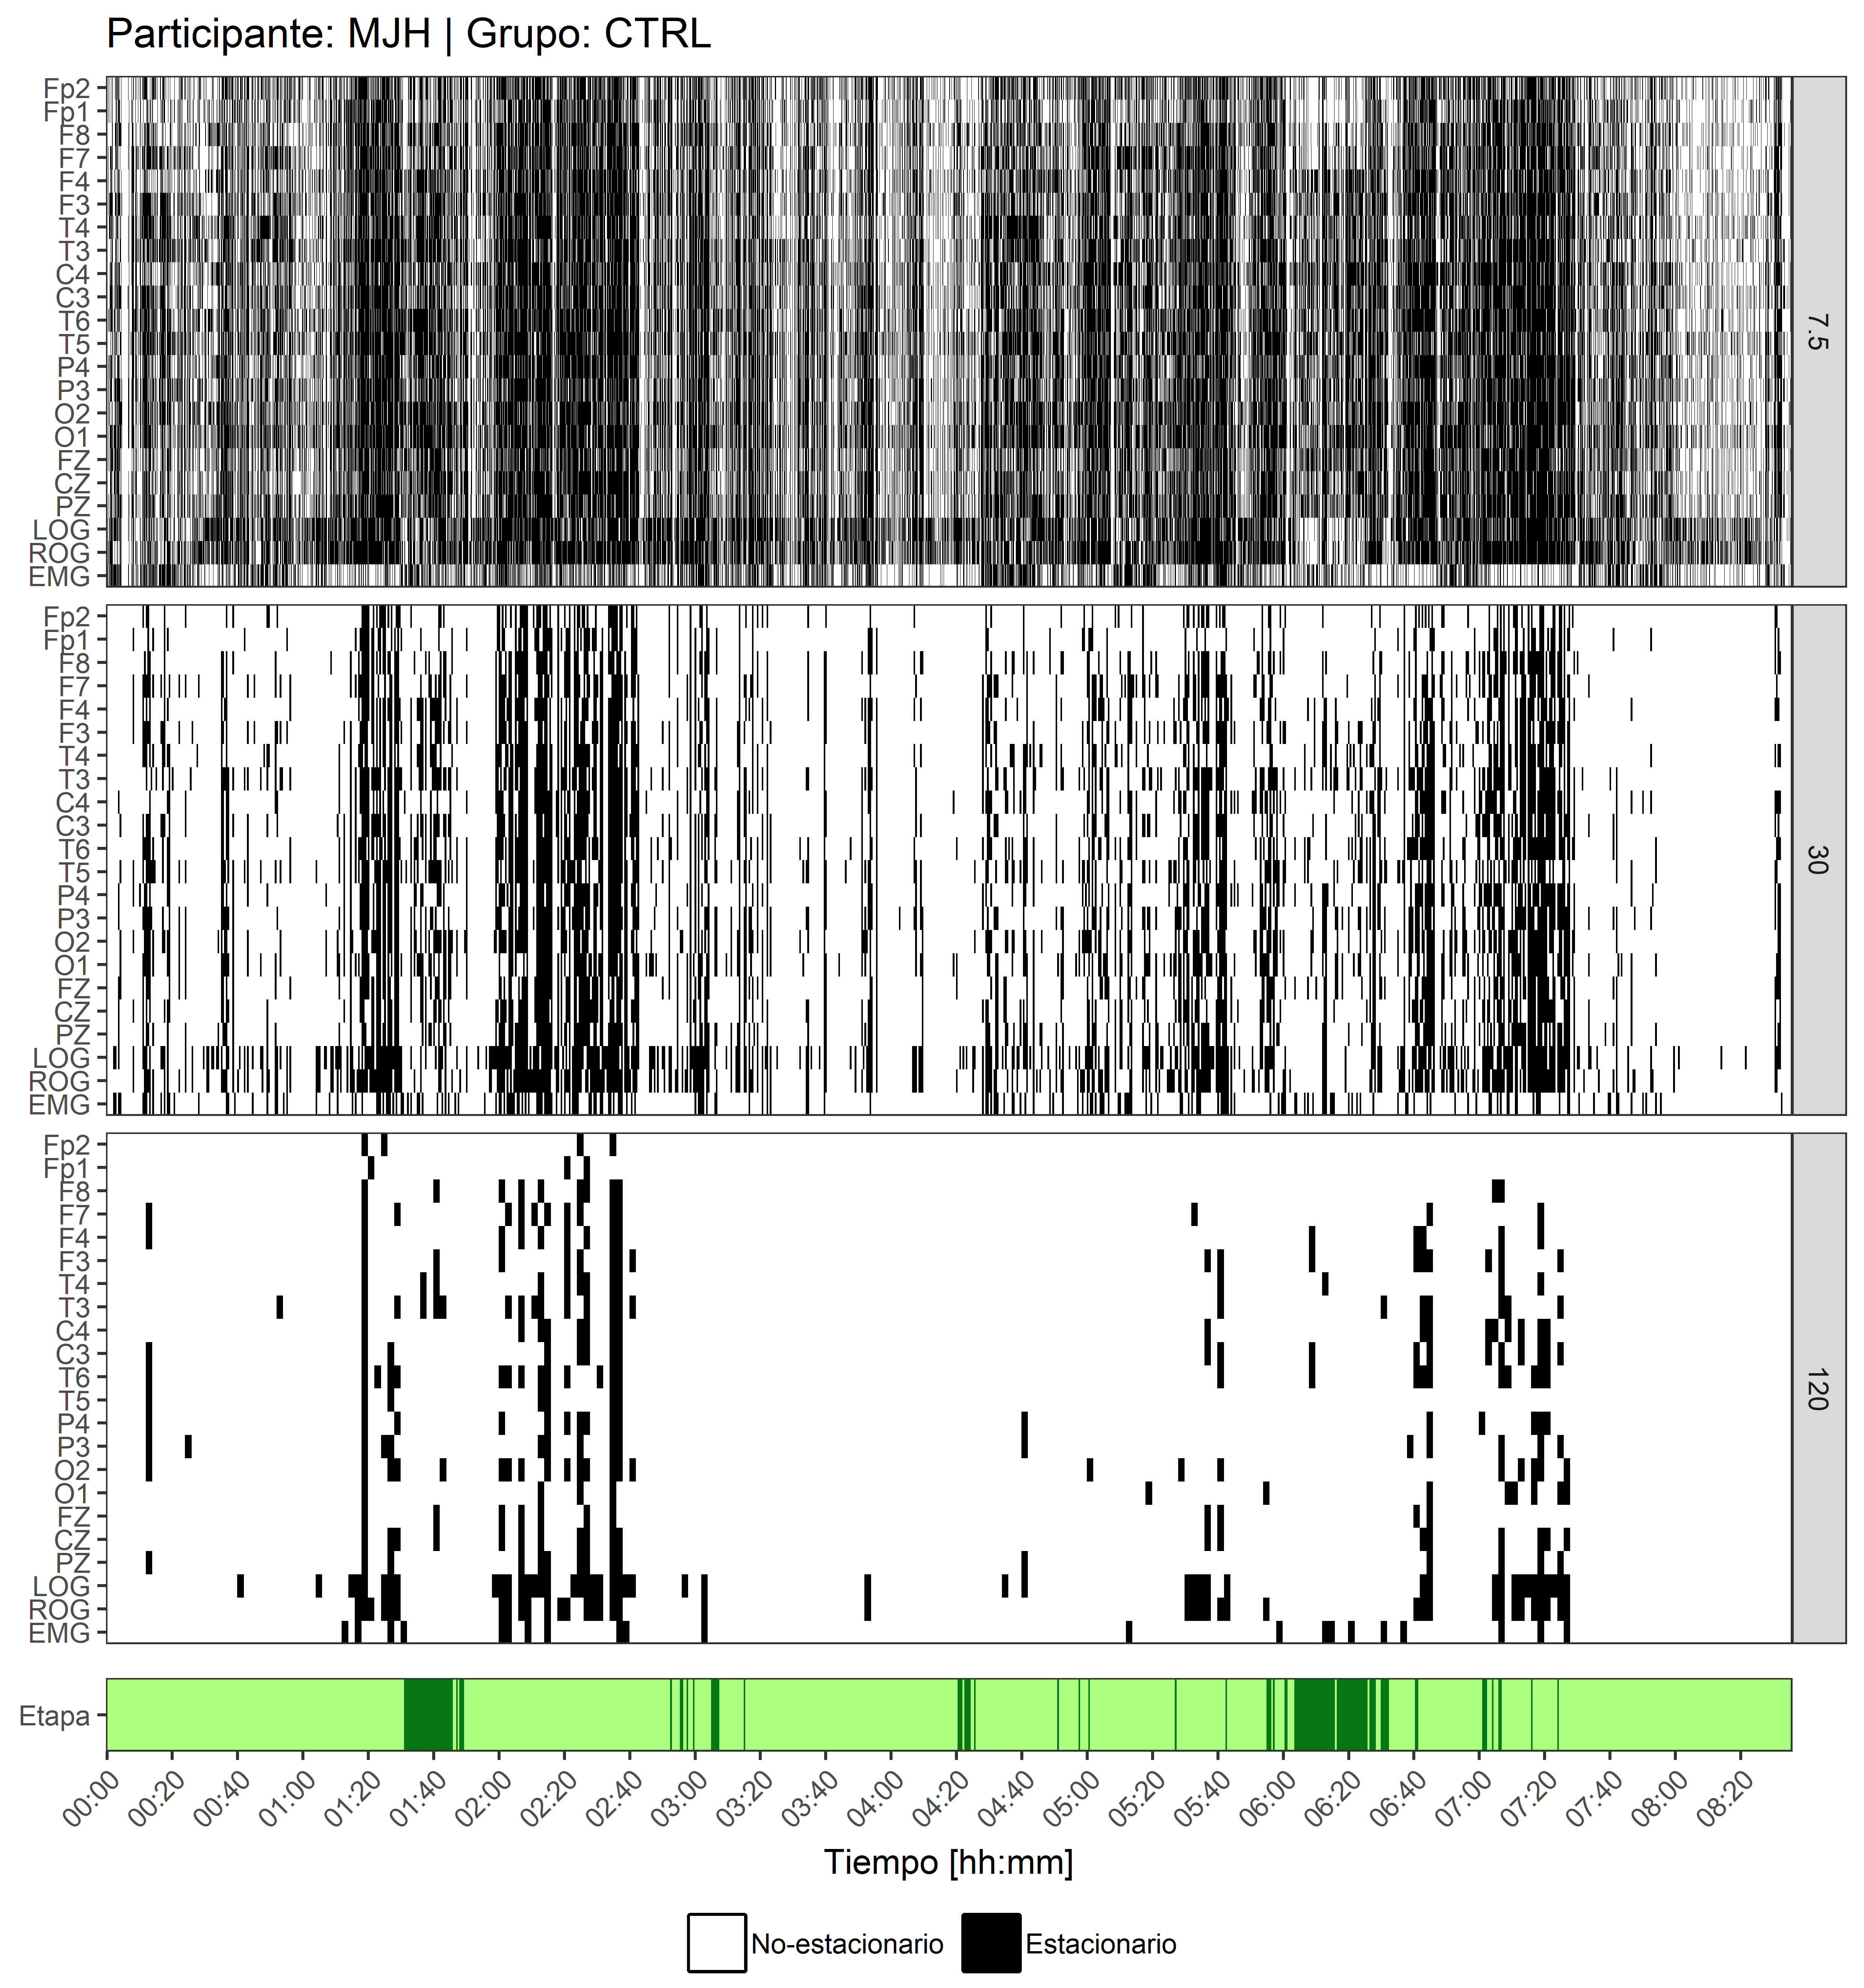
\includegraphics[width=\linewidth]
{./scripts_graf_res/MJNNVIGILOS_patrones_show.png}
\caption[Distribución en el tiempo de las ventanas clasificadas como estacionarias, considerando diferentes tamaños de ventana]{Distribución en el tiempo de las ventanas clasificadas como estacionarias, considerando diferentes tamaños de ventana. 
Cada ventana fue representada en una cuadrícula según su derivación (margen izquierdo) y momento (margen inferior) de procedencia; posteriormente fue \textit{coloreada} según su clasificación como estacionaria.
Dado que la clasificación de estacionariedad se repitió usando diversos tamaños de ventana, en el margen derecho se indica el tamaño de la ventana en segundos.
En la parte inferior se representan las mismas épocas en su clasificación según etapa de sueño.
%Adicionalmente, en la parte superior se indican los \textit{patrones emergentes} de estacionariedad; para más detalles al respecto, ver el texto.
}
\label{img:patrones}
\end{figure}

Los gráficos obtenidos mediante este procedimiento mostraron algunas regularidades que merecen especial atención: \textit{bloques emergentes} de épocas que comparten clasificación como estacionarias (o como no--estacionarias).
%
Estos bloques identificados visualmente se extienden entre diversas derivaciones; puede verse un ejemplo de ello en la figura \ref{img:patrones}.
%
Debido a la forma en que se efectuó la clasificación de estacionariedad (usando la prueba de PSR) puede garantizarse que estos patrones emergentes no son producidos por la clasificación per se.
%
Se hipotetiza que estos \textit{patrones de estacionariedad}
corresponden a las diferentes etapas de sueño.
%
%Posteriormente se discutirá con más detalle al respecto.

Dentro del contexto del PDCL en adultos mayores, estos patrones de estacionariedad no serán definidos formalmente ni estudiados detalladamente; se presentan como un hallazgo incidental y como verificación empírica de las capacidades de la técnica descrita para distinguir características que varían en el tiempo.
%
%Esta decisión fue tomada considerando la naturaleza fuertemente cualitativa de dichos patrones.

\subsection*{Efecto de la estacionariedad local}

El procedimiento de graficación se repitió para las clasificaciones de estacionariedad obtenidas usando diferentes tamaños de ventana, con el fin de verificar si la presencia de los bloques podría atribuirse al tamaño de ventana usado.
%
Se encontró que los patrones aparecen con mayor o menor \textit{nitidez} en los gráficos obtenidos usando diferentes tamaños de ventana, tal como se ilustra en la figura \ref{img:patrones}.

%%%%%%%%%%%%%%%%%%%%%%%%%%%%%%%%%%%%%%%%%%%%%%%%%%%%%%%%%%%%%%%%%%%%%%%%%%%%%%%%%%%%%%%%%%%%%%%%%%%

\section{Análisis a nivel de grupo}

Para fines de esta subsección, se ha supuesto que las proporciones de épocas estacionarias durante MOR y NMOR ($\text{p}_{\text{MOR}}$ y $\text{p}_{\text{NMOR}}$) son características intrínsecas de cada individuo. 
%
En otras palabras, si se repite el registro de PSG para el mismo individuo y bajo condiciones similares, y se realiza el mismo procedimiento de segmentación y clasificación de épocas, entonces se espera que las cantidades $\text{p}_{\text{MOR}}$ y $\text{p}_{\text{NMOR}}$ serán las mismas.
%
Este supuesto se basa en que las fases de sueño son \textit{casi indistinguibles} entre diferentes individuos con características similares, y más aún entre diferentes jornadas de sueño para el mismo individuo.
%; para un estudio más detallado de estas últimas afirmaciones, consultar el libro \textit{``Psicofisiología del sueño"} \cite{Corsi1983}.

Con base a los resultados de la subsección anterior, se puede afirmar intuitivamente que la metodología descrita \textit{percibe} parte de algunas fases (o subfases) de sueño, las cuales son comunes entre individuos.
%
Sin embargo, aun si tales observaciones fueran verificadas rigurosamente, el supuesto de que $\text{p}_{\text{MOR}}$ y $\text{p}_{\text{NMOR}}$ son características individuales debería ser verificado por separado.
%
Debido a las limitaciones del presente trabajo --especialmente el tamaño muestral reducido y la limitación de un registro por participante-- el supuesto será usado como tal, y no se verificará debido a la falta de datos.
%
En consecuencia, los resultados en la presente subsección se presentan como \textit{indicios}, con la idea de explorarlos en trabajos futuros.

Entonces bien, las cantidades $\text{p}_{\text{MOR}}$ y $\text{p}_{\text{NMOR}}$, calculadas por separado para todos los participante y todas las derivaciones consideradas, fueron tratados como características que se distribuyen de forma aproximadamente normal sobre las poblaciones que representan los grupos CTRL y PDCL.
%
Se efectuó un ANOVA de dos vías para observar los cambios sobre $\text{p}_{\text{MOR}}$ y $\text{p}_{\text{NMOR}}$ debidos al grupo y la etapa de sueño, cuyos resultados se muestran en el cuadro \ref{tabla:anova_prop}.
%
Se encontró que no hay interacciones significativas entre los factores de etapa y grupo para ninguna derivación; así mismo se encontró que hay diferencias significativas para las derivaciones Fp2, F7, LOG y ROG que pueden ser explicadas por el \textit{efecto} de la etapa se sueño, y de forma similar para las derivaciones LOG y ROG con el efecto de `grupo'.

Las diferencias para LOG y ROG, debidas al efecto de `etapa de sueño', puede explicarse perfectamente por la presencia característica de movimientos oculares rápidos en el sueño MOR. 
%
Este resultado es consistente con una de las tres características que determinan al sueño MOR: atonía muscular, movimientos oculares rápidos y actividad en el EEG de amplitud baja y frecuencias mixtas.
%
Paralelamente estos resultados sugieren que este procedimiento podría ser usado para identificar de forma objetiva y automatizada parte del sueño MOR; 
%si bien esto no es objetivo del presente trabajo, es un hallazgo fortuito.
en el presente trabajo se expone como preliminar, y requiere de un estudio más riguroso para su uso clínico.

Las diferencias en Fp2 y F7 requieren una explicación más cautelosa, ya que el efecto es significativo en la región frontal, la cual típicamente es asociada con la toma de decisiones; sin embargo, la \textit{significancia} es débil y no es consistente sobre la región frontal.
%
Para explorar más a fondo los resultados de la ANOVA, en la figura \ref{comparacion_verde} se han graficado (como diagramas de caja) los valores $\text{p}_{\text{MOR}}$ y $\text{p}_{\text{NMOR}}$ muestrales; se observa que, intuitivamente, las cantidades $\text{p}_{\text{MOR}}$ y $\text{p}_{\text{NMOR}}$ son muy diferentes entre grupos y entre etapas, pero que posiblemente no resultan significativas debido a la gran variabilidad dentro de las categorías.
%
En principio, es posible justificar dicha falla por el tamaño reducido del grupo muestral.

Con respecto a las diferencias entre grupos para las derivaciones LOG y ROG, puede decirse que recientemente se ha sugerido que es posible detectar diferencias entre sujetos con y sin DCL usando registros de --entre otras derivaciones-- movimientos oculares \cite{FRONTIERS}.

{
\setlength\tabcolsep{3pt}
\begin{table}
\centering
\caption{ANOVA para los efectos Grupo y Etapa de sueño sobre las cantidades $\text{p}_{\text{MOR}}$ y $\text{p}_{\text{NMOR}}$.}
\label{tabla:anova_prop}
\begin{small}
\begin{tabular}{lllllllllllllrllrllrl}
\toprule
 & \multicolumn{5}{l}{CTRL} &  & \multicolumn{5}{l}{PDCL} &  & \multicolumn{8}{l}{ANOVA} \\
\cmidrule{2-6} \cmidrule{8-12} \cmidrule{14-21}
 & \multicolumn{2}{l}{NMOR} &  & \multicolumn{2}{l}{MOR} &  & \multicolumn{2}{l}{NMOR} &  & \multicolumn{2}{l}{MOR} &  & \multicolumn{2}{l}{Grupo} &  & \multicolumn{2}{l}{Etapa} &  & \multicolumn{2}{l}{G$\times$E} \\
\cmidrule{2-3} \cmidrule{5-6} \cmidrule{8-9} \cmidrule{11-12} \cmidrule{14-15} \cmidrule{17-18} \cmidrule{20-21} 
 & M & DE & & M & DE & & M & DE & & M & DE & & F & p & & F & p & & F & p \\
\midrule
Fp2 & 17.2 & 4.0  &  & 6.3  & 5.8  &  & 10.6 & 8.4  &  & 3.7  & 7.0  &  & 2.08 & .171 &  & 7.51  &\bf .016 &  & 0.40 & .537 \\
Fp1 & 17.5 & 9.0  &  & 9.1  & 11.5 &  & 10.8 & 10.5 &  & 4.5  & 7.7  &  & 1.53 & .237 &  & 2.48  & .138 &  & 0.05 & .829 \\
F8  & 19.3 & 7.6  &  & 14.7 & 13.3 &  & 12.5 & 7.8  &  & 8.9  & 14.0 &  & 1.43 & .252 &  & 0.60  & .453 &  & 0.01 & .918 \\
F7  & 19.0 & 5.0  &  & 7.7  & 7.6  &  & 12.6 & 9.6  &  & 5.5  & 10.6 &  & 1.09 & .314 &  & 4.81  &\bf .046 &  & 0.25 & .621 \\
F4  & 20.0 & 5.5  &  & 16.2 & 14.5 &  & 14.4 & 12.5 &  & 15.2 & 15.1 &  & 0.30 & .595 &  & 0.04  & .836 &  & 0.14 & .716 \\
F3  & 19.9 & 4.0  &  & 14.4 & 9.9  &  & 15.1 & 13.8 &  & 17.1 & 23.0 &  & 0.02 & .890 &  & 0.03  & .858 &  & 0.27 & .610 \\
T4  & 22.4 & 7.6  &  & 21.2 & 17.1 &  & 16.2 & 7.8  &  & 26.2 & 19.0 &  & 0.01 & .926 &  & 0.57  & .461 &  & 0.71 & .414 \\
T3  & 27.2 & 6.6  &  & 28.1 & 14.8 &  & 18.7 & 9.5  &  & 24.5 & 20.7 &  & 0.79 & .390 &  & 0.28  & .603 &  & 0.13 & .726 \\
C4  & 29.4 & 7.9  &  & 23.2 & 15.9 &  & 16.9 & 12.4 &  & 25.6 & 18.8 &  & 0.53 & .481 &  & 0.09  & .772 &  & 1.15 & .301 \\
C3  & 25.5 & 5.4  &  & 24.8 & 11.5 &  & 18.8 & 12.2 &  & 25.0 & 18.0 &  & 0.28 & .604 &  & 0.27  & .614 &  & 0.31 & .585 \\
T6  & 31.5 & 10.5 &  & 24.1 & 15.1 &  & 17.0 & 9.3  &  & 25.0 & 21.0 &  & 0.94 & .349 &  & 0.03  & .871 &  & 1.20 & .292 \\
T5  & 29.4 & 16.7 &  & 33.7 & 23.1 &  & 22.2 & 14.9 &  & 32.0 & 17.8 &  & 0.27 & .612 &  & 0.74  & .403 &  & 0.10 & .755 \\
P4  & 25.8 & 6.0  &  & 20.1 & 13.4 &  & 15.8 & 10.0 &  & 22.7 & 19.4 &  & 0.33 & .576 &  & 0.04  & .843 &  & 0.95 & .345 \\
P3  & 25.6 & 9.7  &  & 22.7 & 13.8 &  & 18.7 & 10.1 &  & 28.6 & 19.0 &  & 0.01 & .939 &  & 0.42  & .526 &  & 0.93 & .350 \\
O2  & 27.2 & 7.8  &  & 24.3 & 18.1 &  & 18.3 & 11.2 &  & 25.5 & 21.0 &  & 0.26 & .615 &  & 0.13  & .721 &  & 0.47 & .506 \\
O1  & 27.8 & 9.5  &  & 29.1 & 20.9 &  & 17.5 & 11.7 &  & 25.3 & 20.6 &  & 0.81 & .383 &  & 0.40  & .539 &  & 0.17 & .685 \\
FZ  & 23.4 & 3.1  &  & 24.2 & 10.9 &  & 16.8 & 13.9 &  & 21.5 & 17.8 &  & 0.55 & .469 &  & 0.24  & .634 &  & 0.10 & .758 \\
CZ  & 22.5 & 6.2  &  & 18.7 & 11.1 &  & 16.4 & 12.0 &  & 17.8 & 12.7 &  & 0.46 & .510 &  & 0.03  & .865 &  & 0.24 & .633 \\
PZ  & 22.9 & 4.9  &  & 17.6 & 10.0 &  & 16.0 & 11.9 &  & 23.0 & 17.7 &  & 0.02 & .904 &  & 0.07  & .797 &  & 1.06 & .321 \\
LOG & 50.5 & 10.3 &  & 22.9 & 13.2 &  & 34.3 & 8.9  &  & 9.4  & 9.6  &  & 9.10 &\bf .009 &  & 28.19 &\bf .000 &  & 0.08 & .786 \\
ROG & 54.2 & 14.9 &  & 30.5 & 17.3 &  & 34.2 & 17.1 &  & 14.3 & 13.3 &  & 5.89 &\bf .029 &  & 8.53  &\bf .011 &  & 0.07 & .800 \\
EMG & 15.1 & 8.2  &  & 16.2 & 9.4  &  & 6.8  & 7.4  &  & 13.9 & 16.6 &  & 0.99 & .337 &  & 0.68  & .423 &  & 0.31 & .588 \\
\bottomrule 
\multicolumn{20}{l}{M=media muestral; DE=Desviación estándar; G$\times$E=interacción Grupo y Etapa}
\end{tabular}
\end{small}
\end{table}
}

\begin{figure}
\centering
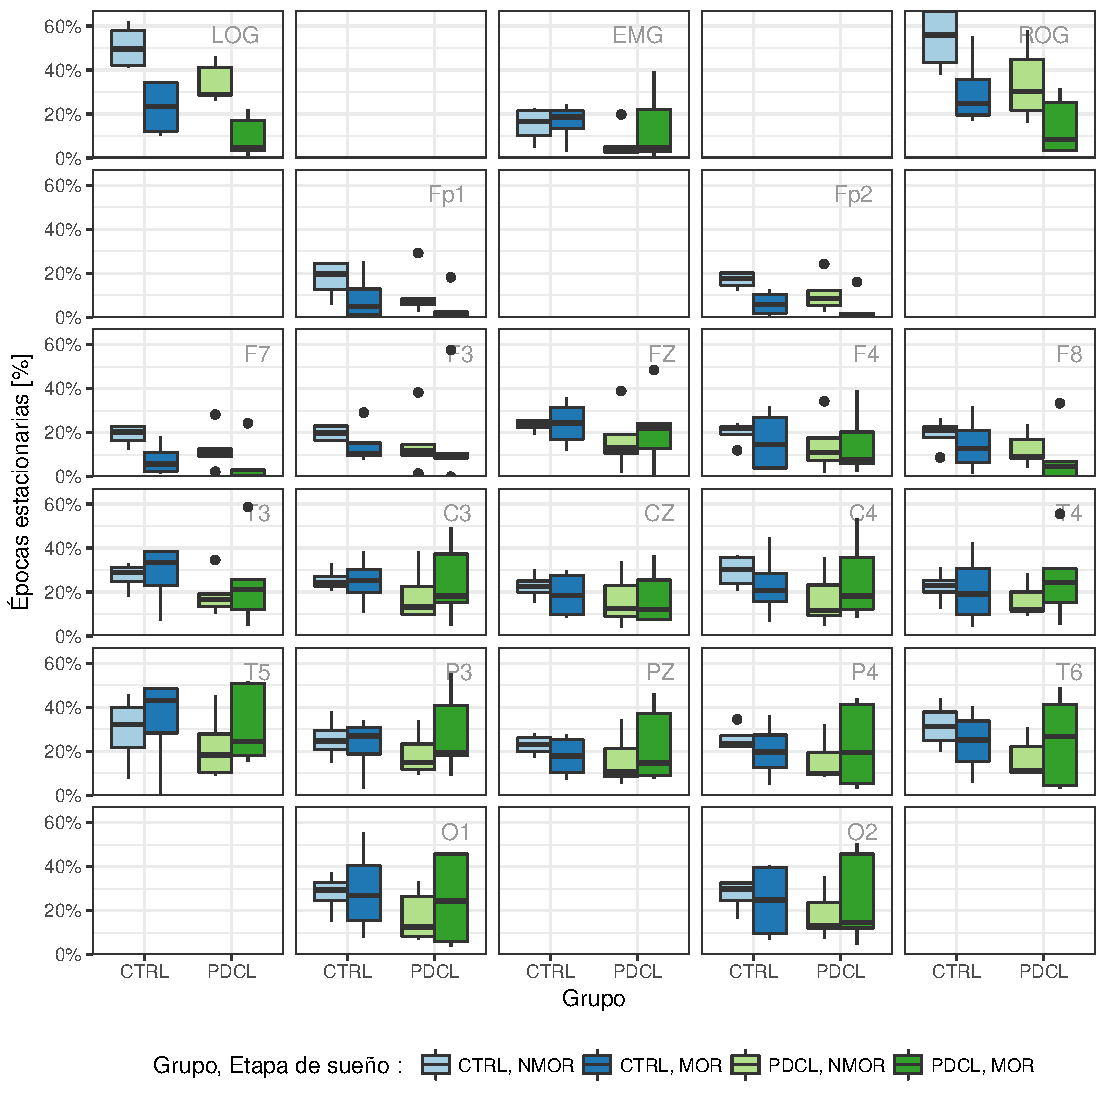
\includegraphics[width=\linewidth]
{./scripts_graf_res/comparacion_cabeza.pdf}
\caption{Proporciones de épocas estacionarias, durante sueño MOR y NMOR y para todas las derivaciones.
%
Los puntos representan valores \textit{atípicos}, según su definición para diagramas de caja.
%; es decir, aquellos valores fuera del intervalo $[Q_1-1.5 R, Q_3 + 1.5 R]$, con $Q_1$ y $Q_3$ el primero y tercer cuartiles muestrales y $R=Q_3-Q_1$.
%
Los asteriscos indican en qué derivaciones se hallaron \textit{efectos} significativos usando una ANOVA de dos factores: `etapa de sueño' y `grupo'; el efecto de `etapa de sueño' fue significativo para Fp2, F7, LOG y ROG, mientras que el efecto `grupo' fue significativo para LOG y ROG.
%
La posición de cada gráfico se corresponden con aquellos de la figura \ref{img:estampa}.}
\label{comparacion_verde}
\end{figure}

%\begin{figure}
%\centering
%\includegraphics[width=\linewidth]
%{./img_art_dfa/Comparacion_gpos_CTL_PDC_v3.pdf}
%\caption{Proporciones de épocas estacionarias, durante sueño MOR y NMOR.}
%\label{comparacion_verde}
%\end{figure}
%
%\begin{figure}
%\centering
%\includegraphics[width=\linewidth]
%{./img_art_dfa/Comparacion_gpos_MOR_NMOR_v3.pdf}
%\caption{Proporciones de épocas estacionarias, grupos CTL y PDC.}
%\label{comparacion_graf}
%\end{figure}

%%%%%%%%%%%%%%%%%%%%%%%%%%%%%%%%%%%%%%%%%%%%%%%%%%%%%%%%%%%%%%%%%%%%%%%%%%%%%%%%%%%%%%%%%%%%%%%%%%%
%%%%%%%%%%%%%%%%%%%%%%%%%%%%%%%%%%%%%%%%%%%%%%%%%%%%%%%%%%%%%%%%%%%%%%%%%%%%%%%%%%%%%%%%%%%%%%%%%%%
%%%%%%%%%%%%%%%%%%%%%%%%%%%%%%%%%%%%%%%%%%%%%%%%%%%%%%%%%%%%%%%%%%%%%%%%%%%%%%%%%%%%%%%%%%%%%%%%%%%
%%%%%%%%%%%%%%%%%%%%%%%%%%%%%%%%%%%%%%%%%%%%%%%%%%%%%%%%%%%%%%%%%%%%%%%%%%%%%%%%%%%%%%%%%%%%%%%%%%%

%%%%%%%%%%%%%%%%%%%%%%%%%%%%%%%%%%%%%%%%%%%%%%%%%%%%%%%%%%%%%%%%%%%%%%%%%%%%%%%%%%%%%%%%%%%%%%%%%%%
%%%%%%%%%%%%%%%%%%%%%%%%%%%%%%%%%%%%%%%%%%%%%%%%%%%%%%%%%%%%%%%%%%%%%%%%%%%%%%%%%%%%%%%%%%%%%%%%%%%
%%%%%%%%%%%%%%%%%%%%%%%%%%%%%%%%%%%%%%%%%%%%%%%%%%%%%%%%%%%%%%%%%%%%%%%%%%%%%%%%%%%%%%%%%%%%%%%%%%%
%%%%%%%%%%%%%%%%%%%%%%%%%%%%%%%%%%%%%%%%%%%%%%%%%%%%%%%%%%%%%%%%%%%%%%%%%%%%%%%%%%%%%%%%%%%%%%%%%%%

\chapter{Discusión y Conclusiones}

%Considerar a las épocas, fragmentos de registros electrofisiológicos, como unidades de estudio es equivalente a considerar como unidades de estudio a las sub-capas que componen a la corteza cerebral.

Como se discutió en la sección \ref{sec:est_local}, la base de este trabajo es la hipótesis 
%(que en el presente trabajo se manejó como supuesto) 
de que el cerebro es un sistema complejo, cuya actividad se comporta como una secuencia organizada de fragmentos de actividad \textit{simple}.
%
Tal característica es referida como \textbf{estacionariedad local}, y la hipótesis descrita es que la actividad cerebral es localmente estacionaria.

En el presente trabajo la `hipótesis de estacionariedad local' fue manejada como un supuesto, y se hipotetizó de que el DCL --o más en concreto, el PDCL-- \textit{afecta} la organización de la actividad cerebral respecto a la forma en que aparecen fragmentos de actividad simple.
%
De forma concreta, se decidió usar a la estacionariedad débil para declarar que los registros analizados son simples; de forma aún más concreta, se usó la prueba de estacionariedad débil de Priestley y Subba Rao para declarar si los registros analizados son débilmente estacionarios.

Conviene comentar que se eligió usar la estacionariedad débil porque es una cantidad \textit{sencilla}, que se usualmente se asume pero no se verifica, y porque una gran cantidad de métodos de análisis la usan (esto será discutido más adelante).
%
%Así mismo, conviene mencionar que se ha usado la técnica de PSG para garantizar que los participantes no presentan acti.

Para facilitar la notación, se definieron las cantidades $\text{p}_{\text{MOR}}$ y $\text{p}_{\text{NMOR}}$, que representan la proporción de épocas durante las cuales los fragmentos de registro de PSG (sinónimo de épocas) \textit{son} débilmente estacionarios\footnote{Los registros de PSG son interpretados como observaciones de procesos estocásticos semi-estacionarios (ver definición \ref{def:semi_estacionario}); se dice que un fragmento de registro de PSG es débilmente estacionario si se puede rechazar la hipótesis de no--estacionariedad usando la prueba de Priestley--Subba Rao (ver sección \ref{sec:psr}).} durante MOR y NMOR, respectivamente; en otras palabras
\begin{equation}
\text{p}_{\text{MOR}} = \frac{\text{\# épocas estacionarias en MOR}}{\text{\# épocas en MOR}}
\end{equation}
y similarmente para $\text{p}_{\text{NMOR}}$. 
%
Estas cantidades son usadas debido a que la cantidad de épocas en MOR y NMOR son considerablemente diferentes, y así mismo son diferentes la cantidad de épocas en MOR y NMOR para los diferentes participantes.

%Conviene resumir los resultados obtenidos, descritos en el capítulo anterior:
%\begin{itemize}
%\item Al probar la hipótesis $\text{p}_{\text{MOR}} \neq \text{p}_{\text{NMOR}}$ para cada individuo, y posteriormente comparar los resultados entre participantes, no se hallaron patrones de actividad claros.

%\item 
Al probar la hipótesis $\text{p}_{\text{MOR}} \neq \text{p}_{\text{NMOR}}$ a nivel grupal (para lo cual se supuso que estas cantidades se distribuyen normalmente), se  encontró que hay diferencias significativas para las derivaciones Fp2, F7, LOG y ROG que pueden ser explicadas por el \textit{efecto} de la etapa se sueño, y de forma similar para las derivaciones LOG y ROG con el efecto de `grupo'.

%\item 
Se describió una metodología con la cual, usando la clasificación de estacionariedad, se identificaron patrones de actividad que parecen \textit{responder} a las etapas de sueño.
%
Este enfoque no fue explorado más a fondo, pero proporciona evidencia \textit{a favor} de la hipótesis de estacionariedad local.

%\item Cabe destacar que la evidencia aportada indica que el PSG es un conjunto de señales que se comportan como no-estacionarias durante la mayor parte del sueño, lo cual confirma el supuesto usual de que las señales de origen biológico son por naturaleza no-estacionarias. 
%\end{itemize}

Las diferencias halladas en LOG y ROG pueden ser explicadas por las características del sueño MOR, ya que los movimientos oculares rápidos son una característica distintiva del sueño MOR --y que le dan nombre.

Por otro lado, las diferencias en Fp2 y F7 son \textit{prometedoras} porque el lóbulo frontal se asocia típicamente a funciones cognitivas; el nivel de significancia es débil, pero ello puede ser debido a que la muestra es relativamente pequeña.
%
Por ejemplo, en \cite{FRONTIERS} se usa un número ligeramente mayor de individuos junto otro método de análisis, obteniéndose resultados similares.




En necesario mencionar que hay una vasta cantidad de estudios que han explorado la posible relación entre trastornos del sueño y marcadores de daño neuronal o de actividad cerebral anómala \cite{porter15}.
%
De manera generalizada, dichos estudios han sido criticados por deficiencias metodológicas; entre ellos se encuentra el uso de grupos muestrales muy reducidos, de la auto-percepción por los pacientes como parámetro de medición, o incluso de pruebas neuropsicológicas con baja sensibilidad como el MMSE \cite{scullin15}.

%En este contexto cabe comentar, como experiencia personal, que el uso de grupos muestrales pequeños responde principalmente a la situación social y económica en que se encuentran los adultos mayores, especialmente ante los estereotipos asociados al deterioro cognitivo.

Vale la pena mencionar que, como {contramedida} ante el efecto de grupos reducidos, se suele otorgar cierto \textit{prestigio} a las llamadas \textit{técnicas objetivas}, es decir, aquellas que son independientes del examinador.
%
La denominación de `técnicas objetivas' engloba, por ejemplo, a todos los registros electrofisiológicos y sus respectivos análisis cuantitativos (en contraparte a los análisis cualitativos); también es importante que se excluye la auto-percepción de deficiencias cognoscitivas, y las encuestas que no son suficientemente \textit{formales}.
%
%: como los registros de EEG o los análisis sobre sus características; las técnicas objetivas se definen ) con respecto a técnicas subjetivas (como la auto-percepción de fallas cogniscitivas).
%
Como consecuencia de lo anterior, se suele considerar que es posible extraer información fiable de grupos pequeños si se usan herramientas de análisis objetivas; como ejemplo está la revisión hecha por Yan Ma \cite{ma18}, donde predominan grupos relativamente pequeños.







%En base a estos resultados, puede concluirse que los cambios en la corteza cerebral durante el PDCL no inducen cambios significativos en su \textit{comportamiento} como estacionarios;
%en otras palabras, con el PDCL la actividad mantiene una parte importante de su \textit{estructura} y es false que se vuelve más \textit{simple}.

Cabe destacar, como comentario, que la evidencia aportada \textit{apoya} a la hipótesis de estacionariedad local y confirma el supuesto usual de que las señales de origen biológico son por naturaleza no-estacionarias; este resultado es importante para trabajos posteriores usando registros de PSG.

%En el apéndice X se explica que si disminuye el tamaño de época el test de PSR disminuye su 
%potencia, de modo que es más propensa a dar falsos negativos (rechazar la hipótesis de 
%estacionariedad cuando debía aceptarse); entonces, en épocas más pequeñas debería haber más épocas 
%clasificadas como no-estacionarias.
%Sin embargo, al \textit{graficar} la estacionariedad para diferentes tamaños de época (figura
%\ref{comp_VCR}) ocurre que es más frecuente el efecto contrario.

%Se propone que este efecto puede ser explicado si los registros de PSG son \textbf{localmente
%estacionarios}, una propiedad introducida por Dahlhaus \cite{Dahlhaus97} y que consiste en que un
%proceso no-estacionario pueda ser aproximado a trozos \textit{ensamblando} procesos estacionarios
%definidos para intervalos pequeños de tiempo.
%Esta caracterización del EEG ha sido usada anteriormente de manera fructífera pero problemática
%[??].
%
%En el contexto particular del presente trabajo, la presencia de estacionariedad local puede ser
%explicada fisiológicamente por el contenido heterogéneo de ritmos cerebrales de las etapas de 
%sueño; como ejemplo, en la etapa N3 aparecen husos de sueño mezcladas con ritmos Alfa, de modo
%que es posible hallar un fragmento de época en sueño N3 con únicamente un tren de ondas Alfa
%o un tren de husos de sueño.
%Este fenómeno es ilustrado de manera esquemática en la figura \ref{epocas_diferentes}.

%%%%%%%%%%%%%%%%%%%%%%%%%%%%%%%%%%%%%%%%%%%%%%%%%%%%%%%%%%%%%%%%%%%%%%%%%%%%%%%%%%%%%%%%%%%%%%%%%%%
%%%%%%%%%%%%%%%%%%%%%%%%%%%%%%%%%%%%%%%%%%%%%%%%%%%%%%%%%%%%%%%%%%%%%%%%%%%%%%%%%%%%%%%%%%%%%%%%%%%

\section{Conclusiones}

%Es necesario mencionar que, de manera generalizada, muchos estudios han sido criticados por deficiencias metodológicas; entre ellos se encuentra el uso de grupos muestrales muy reducidos, de la auto-percepción por los pacientes como parámetro de medición, o incluso de pruebas neuropsicológicas con baja sensibilidad como el MMSE \cite{scullin15}.%

Se ha reportado que los cambios debidos al DCL están asociados con cambios en la estructura del sueño, y en particular en la etapa MOR.
%
Los resultados obtenidos indican que la clasificación de fragmentos de PSG como estacionarios responde a los cambios entre etapas de sueño, en particular al MOR y también entre los grupos.

%Sin embargo, no se pudo establecer una relación clara entre el PDCL (una forma \textit{concreta} del DCL) y los cambios detectados usando la clasificación de estacionariedad.

%Se concluye que la metodología descrita no puede usarse directamente como un marcador para el diagnóstico del PDCL.

Sin embargo, tampoco puede descartarse su utilidad para dicho fin, ya que muestra diferencias significativas para los patrones de actividad cerebral en la región frontal de la corteza cerebral, la cual se considera fisiológicamente relevante y tradicionalmente es asociada con la toma de decisiones.


Respecto a la hipótesis de estacionariedad local (presentada en la sección \ref{sec:est_local}), la información recabada sugiere que dicha hipótesis se verifica para registros de PSG en adultos mayores.
%
%En otras palabras, es posible que existan fragmentos arbitrariamente cortos de registros de PSG, los cuales no \textit{corresponden} a procesos estocásticos débilmente estacionarios.
%
%Paralelamente, los resultados obtenidos sugieren que la presencia de dichos fragmentos se ve influida por la etapa de sueño --o quizá en general por el estado de actividad del cerebro.
%
Se hipotetiza que éste fenómeno explica los resultados {favorables} en dirección a la detección del PDCL \textit{usando},
% la estacionariedad.
%
y que
%Puede especularse que 
un mejor entendimiento de dicho fenómeno podría usarse para 
%mejorar la metodología respecto a la detección el PDCL.
optimizar la metodología descrita.
%
%Como consecuencia directa de este fenómeno, es posible limitar los efectos \textit{distorsivos} de la no-estacionariedad, para lo cual basta un diseño experimental que distinga adecuadamente el estado de actividad a estudiar. 


%Se concluye que es posible la ocurrencia de fragmentos arbitrariamente cortos de registros de PSG que no son débilmente estacionarios. Paralelamente, la presencia de estos fragmentos se ve influida por el estado de actividad del cerebro.
%%
%Como consecuencia directa de este fenómeno, es posible limitar los efectos \textit{distorsivos} de la no-estacionariedad, para lo cual basta un diseño experimental que distinga adecuadamente el estado de actividad a estudiar. 

El hallazgo de patrones emergentes de estacionariedad (ver sección \ref{sec:analisis_registro}) sugiere que, en principio, es posible usar la clasificación de estacionariedad en registros de EEG para caracterizar estados de actividad cerebral. 
%Para ello, falta investigar las características particulares de la etapa que se busca identificar, así como otras etapas cercanas en el tiempo.
%
Esta posibilidad es interesante, pero va más allá de los objetivos del presente trabajo.
 
%  posible usar la proporción de estacionariedad (\textit{densidad} de ventanas estacionarias en el sentido de PSR) en el EEG para caracterizar estados de actividad cerebral. Para ello, falta investigar las características particulares de la etapa que se busca identificar, así como otras etapas cercanas en el tiempo.

%%%%%%%%%%%%%%%%%%%%%%%%%%%%%%%%%%%%%%%%%%%%%%%%%%%%%%%%%%%%%%%%%%%%%%%%%%%%%%%%%%%%%%%%%%%%%%%%%%%
%%%%%%%%%%%%%%%%%%%%%%%%%%%%%%%%%%%%%%%%%%%%%%%%%%%%%%%%%%%%%%%%%%%%%%%%%%%%%%%%%%%%%%%%%%%%%%%%%%%

\section{Trabajo futuro}

Los resultados obtenidos son \textit{prometedores} y preliminares para declarar marcadores clínicos para el PDCL basados en la metodología descrita.
%
En el contexto de la colaboración con el Laboratorio de Sueño, Emoción y Cognición, la metodología será automatizada para poder analizar el total de registros obtenidos en el estudio por Vázquez Tagle y colaboradores.
%
Con base en los resultados obtenidos con un número mayor de participantes, se decidirá si se inicia un nuevo estudio para \textit{validar} la metodología descrita.

%Una vez que se haya identificado un marcador para el PDC usando un grupo de laboratorio, conviene automatizar los análisis para su uso clínico sobre un público más general.
%
%Un uso más amplio de la técnica asegura una mayor población para poder estudiar la efectividad y sensibilidad de la prueba Y más que eso, se espera que puedan ser sinceramente beneficiosos para los pacientes. 
%
%Siguiendo el protocolo usual, los marcadores presentados no serán usados como único recurso para generar un diagnóstico clínico, sino como un apoyo a las herramientas existentes.

De manera general, el uso de marcadores basados en registros de PSG aporta una base objetiva al diagnóstico del deterioro cognitivo, y complementa los resultados más subjetivos de pruebas neuropsicológicas; esta afirmación permanece válida para una gran variedad de señales electrofisiológicas y de trastornos mentales.
%
Conviene destacar que las técnicas basadas en el EEG son relativamente poco \textit{invasivas}, de bajo costo y fácil acceso, con relación a la calidad de la información obtenida y en comparación con otras técnicas para la observación del sistema nervioso central.
%
Entonces, generar marcadores diagnósticos tempranos basados en el EEG facilita su acceso para el público en general, en especial para detectar etapas tempranas del deterioro cognitivo.

En otro ámbito, los patrones emergentes de estacionariedad serán explorados en trabajos futuros.

%%%%%%%%%%%%%%%%%%%%%%%%%%%%%%%%%%%%%%%%%%%%%%%%%%%%%%%%%%%%%%%%%%%%%%%%%%%%%%%%%%%%%%%%%%%%%%%%%%%
%%%%%%%%%%%%%%%%%%%%%%%%%%%%%%%%%%%%%%%%%%%%%%%%%%%%%%%%%%%%%%%%%%%%%%%%%%%%%%%%%%%%%%%%%%%%%%%%%%%
%%%%%%%%%%%%%%%%%%%%%%%%%%%%%%%%%%%%%%%%%%%%%%%%%%%%%%%%%%%%%%%%%%%%%%%%%%%%%%%%%%%%%%%%%%%%%%%%%%%
%%%%%%%%%%%%%%%%%%%%%%%%%%%%%%%%%%%%%%%%%%%%%%%%%%%%%%%%%%%%%%%%%%%%%%%%%%%%%%%%%%%%%%%%%%%%%%%%%%%

\appendix

%%%%%%%%%%%%%%%%%%%%%%%%%%%%%%%%%%%%%%%%%%%%%%%%%%%%%%%%%%%%%%%%%%%%%%%%%%%%%%%%%%%%%%%%%%%%%%%%%%%
%%%%%%%%%%%%%%%%%%%%%%%%%%%%%%%%%%%%%%%%%%%%%%%%%%%%%%%%%%%%%%%%%%%%%%%%%%%%%%%%%%%%%%%%%%%%%%%%%%%
%%%%%%%%%%%%%%%%%%%%%%%%%%%%%%%%%%%%%%%%%%%%%%%%%%%%%%%%%%%%%%%%%%%%%%%%%%%%%%%%%%%%%%%%%%%%%%%%%%%
%%%%%%%%%%%%%%%%%%%%%%%%%%%%%%%%%%%%%%%%%%%%%%%%%%%%%%%%%%%%%%%%%%%%%%%%%%%%%%%%%%%%%%%%%%%%%%%%%%%

\chapter{Puntajes para pruebas neuropsicológicas}
\label{apendice_pruebas}

%En el contexto del presente trabajo fueron usadas varias pruebas neuropsicológicas con el fin de identificar el PDCL (posible deterioro cognitivo leve) en adultos mayores.
%%
%Cabe mencionar que este tipo de pruebas funcionan a nivel de comportamiento, es decir, no pueden detectar cambios en el tejido cerebral o su actividad.

En psicología los instrumentos de medición comunes son las pruebas neuropsicológicas, entendidas como muestras de alguna conducta de interés a las que se asignan puntajes para comparar cuantitativamente a los sujetos \cite{Ardila12}. 
%
%Es a través de estas herramientas que se declaran formalmente las deficiencias cognitivas, así como su severidad y subclasificaciones posteriores.
%
Para fines del presente trabajo, fueron usadas varias pruebas neuropsicológicas con el fin de identificar el PDCL (posible deterioro cognitivo leve) en adultos mayores, además de otras afecciones relacionadas al diagnostico del PDCL.
%
Concretamente, fueron usadas las siguientes pruebas:
\begin{itemize}
\item {Short Anxiety Screening Test (SAST)}. 
\item {Geriatric Depression Scale (GDS)}.
\item {Mini--Mental State Examination (MMSE)}.
\item {Evaluación Neuropsicológica (Neuropsi)}.
\item {Escala sobre las actividades cotidianas de la vida diaria (KATZ)}.
\end{itemize}

Para más información, ver sección \ref{seccion:dcl}.
%
A continuación se presentan únicamente los \textit{puntajes de corte}, puntajes para los cuales la evidencia aportada por las pruebas es indicativa de alguna característica.
%: depende de otros para transportarse, presenta problemas en la memoria de corto plazo, etc.
%
Este material fue retirado del texto principal para facilitar su lectura.

\begin{table}
\centering
\caption{Puntajes de corte para las pruebas SAST y GDS}
\begin{tabular}{lcl}
\toprule
Prueba & Puntaje & Indicación \\
\midrule
SAST
& $>24$ & Positivo para ansiedad \\
& 22 -- 24 & No es conclusivo \\
& $<22$ & Negativo para ansiedad \\
\midrule
GDS
& 0 -- 4 & Normal \\
& 5 -- 8 & Depresión leve \\
& 9 -- 11 & Depresión moderada \\
& 12 -- 15 & Depresión severa \\
\bottomrule
\multicolumn{3}{l}{Fuente: Yesavage \cite{Yesavage82}, Sinoff \cite{sinoff99} }
\end{tabular}
\label{anexo:sast_gds}
\end{table}

\begin{table}
\centering
\caption{Puntuación para la prueba KATZ}
\begin{tabular}{lll}
\toprule
\multicolumn{2}{l}{Actividad} & Descripción \\
\midrule
1 & Baño           & Se baña sólo, o con ayuda para lavarse \\
			      && una parte del cuerpo.\\
2 & Vestido        & Se viste totalmente sin ayuda.\\
3 & Retrete        & Sin ayuda.\\
4 & Movilidad      & Entra y sale de la cama.\\
5 & Continencia    & Control de esfínteres.\\
6 & Alimentación   & Lleva la comida del plato a la boca. \\
\bottomrule
\multicolumn{3}{l}{Fuente: Katz \cite{katz70}. Se puntúa la dependencia para cada actividad.}
\end{tabular}
\label{anexo:katz}
\end{table}
% http://medicina.uc.cl/programa-geriatria/indice-katz-independencia-en-actividades-diarias

\begin{table}
\centering
\caption{Puntajes de corte para la prueba Neuropsi}
\begin{tabular}{llccrccc}
\toprule
&& \multicolumn{2}{l}{Sano} & \phantom{.} & \multicolumn{3}{l}{Deterioro cognitivo} \\
\cmidrule{3-4} \cmidrule{6-8} 
Edad & Escolaridad & Alto & Normal && Leve & Moderado & Severo\\
\midrule
31 -- 50  
& Nula     & 95  & 68  &  & 54  & 41 & 28 \\
& 1 -- 4   & 105 & 81  &  & 69  & 58 & 46 \\
& 5 -- 9   & 118 & 106 &  & 101 & 90 & 79 \\
& 10 -- 24 & 113 & 102 &  & 97  & 88 & 78 \\
\midrule
51 -- 65  
& Nula     & 91  & 59  &  & 44  & 28 & 13 \\
& 1 -- 4   & 98  & 77  &  & 67  & 57 & 47 \\
& 5 -- 9   & 111 & 98  &  & 91  & 79 & 67 \\
& 10 -- 24 & 102 & 93  &  & 88  & 80 & 72 \\
\midrule
66 -- 85  
& Nula     & 76  & 48  &  & 34  & 20 & 6 \\
& 1 -- 4   & 90  & 61  &  & 46  & 32 & 18 \\
& 5 -- 9   & 97  & 80  &  & 72  & 56 & 39 \\
& 10 -- 24 & 92  & 78  &  & 72  & 59 & 46 \\
\bottomrule
\multicolumn{7}{l}{Fuente: Ardila y Ostrosky \cite{Ardila12}}
\end{tabular}
\label{anexo:neuropsi}
\end{table}

\begin{table}
\centering
\caption{Puntajes de corte para la prueba MMSE}
\begin{tabular}{llcc}
\toprule
Edad & Nivel de estudios & Máximo & Deterioro \\
\midrule
45 -- 49&Elemental&23&18 \\
&Primario&26&20 \\
&Medio&28&22 \\
&Superior&29&23 \\
\midrule
50 -- 54&Elemental&23&18 \\
&Primario&27&21 \\
&Medio&28&22 \\
&Superior&29&23 \\
\midrule
55 -- 59&Elemental&22&17 \\
&Primario&26&20 \\
&Medio&28&22 \\
&Superior&29&23 \\
\midrule
60 -- 64&Elemental&23&18 \\
&Primario&26&20 \\
&Medio&28&22 \\
&Superior&29&23 \\
\midrule
65 -- 69&Elemental&22&17 \\
&Primario&26&20 \\
&Medio&28&22 \\
&Superior&29&23 \\
\midrule
70 -- 74&Elemental&22&17 \\
&Primario&25&20 \\
&Medio&27&21 \\
&Superior&28&22 \\
\midrule
75 -- 79&Elemental&21&16 \\
&Primario&25&20 \\
&Medio&27&21 \\
&Superior&28&22 \\
\midrule
80 -- 84&Elemental&20&16 \\
&Primario&25&20 \\
&Medio&25&20 \\
&Superior&27&21 \\
%\midrule
%$>84$&Elemental&19&15 \\
%&Primario&23&18 \\
%&Medio&26&20 \\
%&Superior&27&21 \\
\bottomrule
\multicolumn{2}{l}{Fuente: Folstein \cite{crum93}}
\end{tabular}
\label{anexo:mmse}
\end{table}
%https://www.hipocampo.org/folstein.asp

%%%%%%%%%%%%%%%%%%%%%%%%%%%%%%%%%%%%%%%%%%%%%%%%%%%%%%%%%%%%%%%%%%%%%%%%%%%%%%%%%%%%%%%%%%%%%%%%%%%
%%%%%%%%%%%%%%%%%%%%%%%%%%%%%%%%%%%%%%%%%%%%%%%%%%%%%%%%%%%%%%%%%%%%%%%%%%%%%%%%%%%%%%%%%%%%%%%%%%%
%%%%%%%%%%%%%%%%%%%%%%%%%%%%%%%%%%%%%%%%%%%%%%%%%%%%%%%%%%%%%%%%%%%%%%%%%%%%%%%%%%%%%%%%%%%%%%%%%%%
%%%%%%%%%%%%%%%%%%%%%%%%%%%%%%%%%%%%%%%%%%%%%%%%%%%%%%%%%%%%%%%%%%%%%%%%%%%%%%%%%%%%%%%%%%%%%%%%%%%

%%%%%%%%%%%%%%%%%%%%%%%%%%%%%%%%%%%%%%%%%%%%%%%%%%%%%%%%%%%%%%%%%%%%%%%%%%%%%%%%%%%%%%%%%%%%%%%%%%%
%%%%%%%%%%%%%%%%%%%%%%%%%%%%%%%%%%%%%%%%%%%%%%%%%%%%%%%%%%%%%%%%%%%%%%%%%%%%%%%%%%%%%%%%%%%%%%%%%%%
%%%%%%%%%%%%%%%%%%%%%%%%%%%%%%%%%%%%%%%%%%%%%%%%%%%%%%%%%%%%%%%%%%%%%%%%%%%%%%%%%%%%%%%%%%%%%%%%%%%
%%%%%%%%%%%%%%%%%%%%%%%%%%%%%%%%%%%%%%%%%%%%%%%%%%%%%%%%%%%%%%%%%%%%%%%%%%%%%%%%%%%%%%%%%%%%%%%%%%%

\chapter{Cuadros y figuras adicionales}
\label{apendiceA}

En este apéndice se muestran mayores detalles sobre los resultados obtenidas durante los análisis descritos en el capítulo \ref{ch:metodologia}.
%
Este material fue excluido del texto principal con el fin de agilizar su lectura y enfatizar la interpretación de los resultados en el contexto del PDCL, más que la forma en que fueron calculados.

%Los gráficos \ref{a:cabezas_ctrl} y \ref{a:cabezas_pdcl} representan, esquemáticamente, las derivaciones donde las proporciones de épocas estacionarias son diferentes en MOR y NMOR;, más detalles ver la sección \ref{sec:analisis_epoca}.
%%
%Estos gráficos pueden entenderse como una réplica de la figura \ref{cabeza_new} usando varios tamaños de época.

\section{Total de épocas estacionarias}

En esta subsección se reporta el total de segmentos de PSG clasificados como estacionarios, usando la prueba de PSR.
%
La clasificación se efectuó de manera independiente para todas las derivaciones, y que la misma clasificación se repitió usando diferentes tamaños de ventana; se reportan todos los valores obtenidos.

Adicionalmente se reporta los resultados de aplicar la prueba $\chi^2$ de Pearson para proporciones, usada para verificar si las proporciones de épocas estacionarias durante MOR y NMOR ($\text{p}_{\text{MOR}}$ y $\text{p}_{\text{NMOR}}$) son diferentes.

%\begin{figure}
%\centering
%{\small
%\begin{tabular}{lccccc}
%\toprule
%{\small Tamaño de} & \multicolumn{5}{c}{Grupo CTRL} \\
%    \cmidrule{2-6}
%{\small ventana [s]}    & VCR & MJH & JAE & GHA & MFGR \\
%\midrule
%$30 \times 2^1$ &
%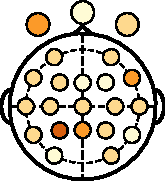
\includegraphics[width=0.13\textwidth]{./img_art_dfa/cabeza_new_VCR_60.pdf} &
%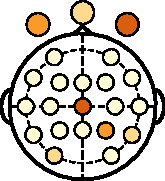
\includegraphics[width=0.13\textwidth]{./img_art_dfa/cabeza_new_MJH_60.pdf} &
%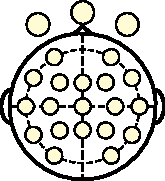
\includegraphics[width=0.13\textwidth]{./img_art_dfa/cabeza_new_JAE_60.pdf} &
%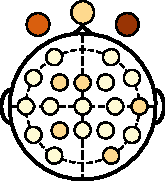
\includegraphics[width=0.13\textwidth]{./img_art_dfa/cabeza_new_GHA_60.pdf} &
%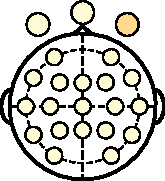
\includegraphics[width=0.13\textwidth]{./img_art_dfa/cabeza_new_MFGR_60.pdf} \\
%\midrule
%$30 \times 2^0$ &
%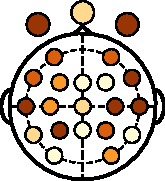
\includegraphics[width=0.13\textwidth]{./img_art_dfa/cabeza_new_VCR_30.pdf} &
%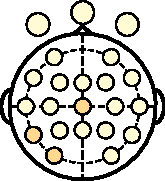
\includegraphics[width=0.13\textwidth]{./img_art_dfa/cabeza_new_MJH_30.pdf} &
%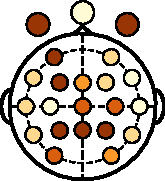
\includegraphics[width=0.13\textwidth]{./img_art_dfa/cabeza_new_JAE_30.pdf} &
%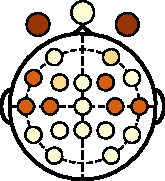
\includegraphics[width=0.13\textwidth]{./img_art_dfa/cabeza_new_GHA_30.pdf} &
%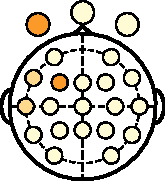
\includegraphics[width=0.13\textwidth]{./img_art_dfa/cabeza_new_MFGR_30.pdf} \\
%\midrule
%$30 \times 2^{-1}$ &
%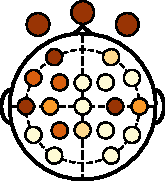
\includegraphics[width=0.13\textwidth]{./img_art_dfa/cabeza_new_VCR_15.pdf} &
%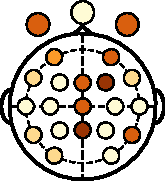
\includegraphics[width=0.13\textwidth]{./img_art_dfa/cabeza_new_MJH_15.pdf} &
%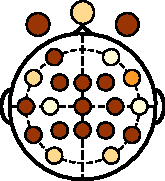
\includegraphics[width=0.13\textwidth]{./img_art_dfa/cabeza_new_JAE_15.pdf} &
%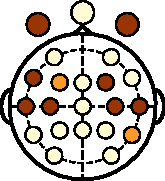
\includegraphics[width=0.13\textwidth]{./img_art_dfa/cabeza_new_GHA_15.pdf} &
%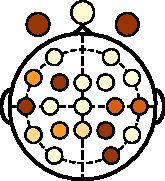
\includegraphics[width=0.13\textwidth]{./img_art_dfa/cabeza_new_MFGR_15.pdf} \\
%\bottomrule
%\end{tabular}\\
%
\includegraphics[scale=.7]{./img_art_dfa/escala.pdf} \\
%}
%\caption{Derivaciones, las cuales la proporción de épocas clasificadas como estacionarias fue significativamente diferente en MOR y NMOR.
%%
%Se han usado diferentes tamaños de ventana.
%%
%La posición de los círculos representan a las derivaciones, en correspondencia con la figura \ref{img:estampa}.}
%\label{a:cabezas_ctrl}
%\end{figure}

%\begin{figure}
%\centering
%{\small
%\begin{tabular}{lccccc}
%\toprule
%{ Tamaño de} & \multicolumn{5}{c}{Grupo PDCL} \\
%    \cmidrule{2-6}
%{ ventana [s]}    & CLO & RLO & RRU & JGZ & AEFP \\
%\midrule
%$30 \times 2^1$ &
%\includegraphics[width=0.13\textwidth]{./img_art_dfa/cabeza_new_CLO_60.pdf} &
%\includegraphics[width=0.13\textwidth]{./img_art_dfa/cabeza_new_RLO_60.pdf} &
%\includegraphics[width=0.13\textwidth]{./img_art_dfa/cabeza_new_RRU_60.pdf} &
%\includegraphics[width=0.13\textwidth]{./img_art_dfa/cabeza_new_JGZ_60.pdf} &
%\includegraphics[width=0.13\textwidth]{./img_art_dfa/cabeza_new_AEFP_60.pdf} \\
%\midrule
%$30 \times 2^0$ &
%\includegraphics[width=0.13\textwidth]{./img_art_dfa/cabeza_new_CLO_30.pdf} &
%\includegraphics[width=0.13\textwidth]{./img_art_dfa/cabeza_new_RLO_30.pdf} &
%\includegraphics[width=0.13\textwidth]{./img_art_dfa/cabeza_new_RRU_30.pdf} &
%\includegraphics[width=0.13\textwidth]{./img_art_dfa/cabeza_new_JGZ_30.pdf} &
%\includegraphics[width=0.13\textwidth]{./img_art_dfa/cabeza_new_AEFP_30.pdf} \\
%\midrule
%$30 \times 2^{-1}$ &
%\includegraphics[width=0.13\textwidth]{./img_art_dfa/cabeza_new_CLO_15.pdf} &
%\includegraphics[width=0.13\textwidth]{./img_art_dfa/cabeza_new_RLO_15.pdf} &
%\includegraphics[width=0.13\textwidth]{./img_art_dfa/cabeza_new_RRU_15.pdf} &
%\includegraphics[width=0.13\textwidth]{./img_art_dfa/cabeza_new_JGZ_15.pdf} &
%\includegraphics[width=0.13\textwidth]{./img_art_dfa/cabeza_new_AEFP_15.pdf} \\
%\bottomrule
%\end{tabular} \\
%\includegraphics[scale=.7]{./img_art_dfa/escala.pdf} \\
%}
%\caption{Derivaciones, las cuales la proporción de épocas clasificadas como estacionarias fue significativamente diferente en MOR y NMOR.
%%
%Se han usado diferentes tamaños de ventana.
%%
%La posición de los círculos representan a las derivaciones, en correspondencia con la figura \ref{img:estampa}.}
%\label{a:cabezas_pdcl}
%\end{figure}

%%%%%%%%%%%%%%%%%%%%%%%%%%%%%%%%%%%%%%%%%%%%%%%%%%%%%%%%%%%%%%%%%%%%%%%%%%%%%%%%%%%%%%%%%%%%%%%%%%%
%%%%%%%%%%%%%%%%%%%%%%%%%%%%%%%%%%%%%%%%%%%%%%%%%%%%%%%%%%%%%%%%%%%%%%%%%%%%%%%%%%%%%%%%%%%%%%%%%%%

\begin{SidewaysTable}
\centering
\caption[Épocas estacionarias y comparación de proporciones, MJH (1/2)]{ Épocas estacionarias según tamaño de ventana, y comparación de sus proporciones entre etapas de sueño; participante MJH (1/2)}
{
\begin{tabular}{lrrclrrclrrclrrc}
\toprule
     & \multicolumn{3}{l}{E = 0.9375 s} &  & \multicolumn{3}{l}{E = 1.875 s} &  & \multicolumn{3}{l}{E = 3.75 s} &  & \multicolumn{3}{l}{E = 7.5 s} \\ 
\cmidrule{2-4} \cmidrule{6-8} \cmidrule{10-12} \cmidrule{14-16}
 & \multicolumn{1}{c}{N+W} & \multicolumn{1}{c}{R} & \multicolumn{1}{c}{$p$} &  & \multicolumn{1}{c}{N+W} & \multicolumn{1}{c}{R} & \multicolumn{1}{c}{$p$} &  & \multicolumn{1}{c}{N+W} & \multicolumn{1}{c}{R} & \multicolumn{1}{c}{$p$} &  & \multicolumn{1}{c}{N+W} & \multicolumn{1}{c}{R} & \multicolumn{1}{c}{$p$} \\
\midrule
Fp2   & 19401     & 2495     & ****    &  & 10125     & 1249    & ****    &  & 4664     & 559     & ****    &  & 1710     & 209    & *       \\
Fp1   & 19529     & 2451     & ****    &  & 10308     & 1229    & ****    &  & 4593     & 551     & ****    &  & 1626     & 201    &         \\
F8    & 19241     & 2762     &         &  & 10434     & 1396    & **      &  & 4930     & 644     & *       &  & 1844     & 266    &         \\
F7    & 18978     & 2679     &         &  & 10580     & 1406    & ***     &  & 5075     & 653     & ***     &  & 1900     & 258    &         \\
F4    & 18211     & 2609     &         &  & 10331     & 1539    & ****    &  & 4970     & 755     & ***     &  & 1908     & 333    & ****    \\
F3    & 18546     & 2665     &         &  & 10494     & 1553    & ****    &  & 5093     & 806     & ****    &  & 1983     & 334    & ****    \\
T4    & 19982     & 2935     & ****    &  & 10866     & 1594    & ***     &  & 5212     & 778     & **      &  & 1981     & 314    & **      \\
T3    & 18556     & 2628     &         &  & 10457     & 1501    &         &  & 5190     & 790     & ****    &  & 2057     & 342    & ****    \\
C4    & 18566     & 2735     & ****    &  & 10709     & 1605    & ****    &  & 5284     & 814     & ****    &  & 2100     & 342    & ****    \\
C3    & 18236     & 2575     &         &  & 10553     & 1522    &         &  & 5194     & 798     & ****    &  & 2083     & 333    & ***     \\
T6    & 18521     & 2696     & **      &  & 10815     & 1581    & **      &  & 5362     & 827     & ****    &  & 2138     & 364    & ****    \\
T5    & 18274     & 2372     & ****    &  & 10160     & 1332    & ****    &  & 5297     & 790     & **      &  & 2205     & 368    & ****    \\
P4    & 18330     & 2709     & ****    &  & 10811     & 1599    & ****    &  & 5228     & 819     & ****    &  & 2087     & 336    & ***     \\
P3    & 18336     & 2558     &         &  & 10665     & 1519    &         &  & 5260     & 796     & ****    &  & 2107     & 334    & ***     \\
O2    & 16418     & 2228     &         &  & 10371     & 1469    &         &  & 5313     & 809     & ****    &  & 2192     & 371    & ****    \\
O1    & 17477     & 2402     &         &  & 10431     & 1407    & *       &  & 5519     & 822     & ***     &  & 2326     & 376    & ****    \\
FZ    & 17630     & 2349     & ***     &  & 10375     & 1515    & *       &  & 5070     & 804     & ****    &  & 1998     & 352    & ****    \\
CZ    & 17430     & 2271     & ****    &  & 10255     & 1467    &         &  & 5144     & 776     & ***     &  & 2041     & 344    & ****    \\
PZ    & 17775     & 2559     &         &  & 10683     & 1551    & *       &  & 5359     & 800     & ***     &  & 2176     & 343    & ***     \\
LOG   & 13116     & 1524     & ****    &  & 8658      & 1122    & ****    &  & 5146     & 608     & ****    &  & 2495     & 292    & ****    \\
ROG   & 17253     & 2493     &         &  & 10092     & 1400    &         &  & 5650     & 734     & ****    &  & 2544     & 313    & ****    \\
EMG   & 18803     & 1533     & ****    &  & 8600      & 697     & ****    &  & 3743     & 293     & ****    &  & 1551     & 204    &         \\
\textbf{Total} & 28987     & 4055     &         &  & 14493     & 2031    &         &  & 7246     & 1016    &         &  & 3623     & 508    &         \\ 
\bottomrule
\end{tabular}
\begin{tabular}{p{18cm}}
E=tamaño de ventana; N+W=NMOR y vigilia; R=MOR; $p$, significancia de la prueba $\chi^{2}$ de Pearson entre las proporciones de ventanas estacionarias en N+W y R: *=0.05, **=0.01, ***=0.005, ****=0.001
\end{tabular}
}
\end{SidewaysTable}
\begin{SidewaysTable}
\centering
\caption[Épocas estacionarias y comparación de proporciones, MJH (2/2)]{ Épocas estacionarias según tamaño de ventana, y comparación de sus proporciones entre etapas de sueño; participante MJH (2/2)}
{
\begin{tabular}{lrrclrrclrrclrrc}
\toprule
     & \multicolumn{3}{l}{E = 15 s} &  & \multicolumn{3}{l}{E = 30 s} &  & \multicolumn{3}{l}{E = 60 s} &  & \multicolumn{3}{l}{E = 120 s} \\ 
\cmidrule{2-4} \cmidrule{6-8} \cmidrule{10-12} \cmidrule{14-16}
 & \multicolumn{1}{c}{N+W} & \multicolumn{1}{c}{R} & \multicolumn{1}{c}{$p$} &  & \multicolumn{1}{c}{N+W} & \multicolumn{1}{c}{R} & \multicolumn{1}{c}{$p$} &  & \multicolumn{1}{c}{N+W} & \multicolumn{1}{c}{R} & \multicolumn{1}{c}{$p$} &  & \multicolumn{1}{c}{N+W} & \multicolumn{1}{c}{R} & \multicolumn{1}{c}{$p$} \\
\midrule
Fp2 & 531  & 67  &      &  & 139 & 12  &   &  & 31  & 2  &   &  & 3   & 1  &  \\
Fp1 & 521  & 58  &      &  & 135 & 11  &   &  & 34  & 4  &   &  & 3   & 0  &  \\
F8  & 623  & 89  &      &  & 187 & 22  &   &  & 48  & 7  &   &  & 9   & 2  &  \\
F7  & 670  & 84  &      &  & 209 & 23  &   &  & 56  & 5  &   &  & 11  & 3  &  \\
F4  & 640  & 124 & **** &  & 196 & 32  &   &  & 58  & 12 &   &  & 13  & 1  &  \\
F3  & 681  & 118 & *    &  & 206 & 37  &   &  & 56  & 10 &   &  & 16  & 1  &  \\
T4  & 662  & 121 & ***  &  & 203 & 34  &   &  & 48  & 11 &   &  & 10  & 3  &  \\
T3  & 765  & 131 & *    &  & 245 & 49  & * &  & 72  & 14 &   &  & 17  & 5  &  \\
C4  & 726  & 128 & **   &  & 225 & 29  &   &  & 62  & 9  &   &  & 15  & 2  &  \\
C3  & 741  & 132 & ***  &  & 226 & 35  &   &  & 61  & 16 &   &  & 17  & 2  &  \\
T6  & 754  & 138 & **** &  & 240 & 40  &   &  & 76  & 16 &   &  & 20  & 4  &  \\
T5  & 818  & 143 & ***  &  & 239 & 48  & * &  & 54  & 12 &   &  & 5   & 2  &  \\
P4  & 727  & 113 &      &  & 222 & 31  &   &  & 59  & 11 &   &  & 14  & 2  &  \\
P3  & 756  & 123 &      &  & 242 & 38  &   &  & 74  & 13 &   &  & 13  & 3  &  \\
O2  & 833  & 139 & *    &  & 248 & 50  & * &  & 81  & 17 &   &  & 20  & 3  &  \\
O1  & 860  & 151 & ***  &  & 251 & 45  &   &  & 73  & 10 &   &  & 10  & 2  &  \\
FZ  & 732  & 129 & **   &  & 211 & 38  &   &  & 56  & 13 &   &  & 10  & 1  &  \\
CZ  & 710  & 121 & *    &  & 211 & 34  &   &  & 63  & 11 &   &  & 15  & 4  &  \\
PZ  & 768  & 119 &      &  & 231 & 31  &   &  & 60  & 9  &   &  & 12  & 3  &  \\
LOG & 1045 & 118 & ***  &  & 373 & 44  &   &  & 137 & 18 &   &  & 39  & 9  &  \\
ROG & 1015 & 114 & ***  &  & 342 & 37  &   &  & 105 & 16 &   &  & 34  & 5  &  \\
EMG & 564  & 94  &      &  & 192 & 31  &   &  & 54  & 14 &   &  & 19  & 2  &  \\
\textbf{Total} & 1811 & 254 &      &  & 905 & 127 &   &  & 436 & 80 & 0 &  & 225 & 33 &  \\
\bottomrule
\end{tabular}
\begin{tabular}{p{14cm}}
E=tamaño de ventana; N+W=NMOR y vigilia; R=MOR; $p$, significancia de la prueba $\chi^{2}$ de Pearson entre las proporciones de ventanas estacionarias en N+W y R: *=0.05, **=0.01, ***=0.005, ****=0.001
\end{tabular}
}
\end{SidewaysTable}


\begin{SidewaysTable}
\centering
\caption[Épocas estacionarias y comparación de proporciones, JAE (1/2)]{ Épocas estacionarias según tamaño de ventana, y comparación de sus proporciones entre etapas de sueño; participante JAE (1/2)}
{
\begin{tabular}{lrrclrrclrrclrrc}
\toprule
     & \multicolumn{3}{l}{E = 0.9375 s} &  & \multicolumn{3}{l}{E = 1.875 s} &  & \multicolumn{3}{l}{E = 3.75 s} &  & \multicolumn{3}{l}{E = 7.5 s} \\ 
\cmidrule{2-4} \cmidrule{6-8} \cmidrule{10-12} \cmidrule{14-16}
 & \multicolumn{1}{c}{N+W} & \multicolumn{1}{c}{R} & \multicolumn{1}{c}{$p$} &  & \multicolumn{1}{c}{N+W} & \multicolumn{1}{c}{R} & \multicolumn{1}{c}{$p$} &  & \multicolumn{1}{c}{N+W} & \multicolumn{1}{c}{R} & \multicolumn{1}{c}{$p$} &  & \multicolumn{1}{c}{N+W} & \multicolumn{1}{c}{R} & \multicolumn{1}{c}{$p$} \\
\midrule
Fp2   & 14507 & 4093 & **** &  & 7993  & 1821 &      &  & 3721 & 706  & **** &  & 1303 & 192 & **** \\
Fp1   & 14347 & 4030 & **** &  & 7442  & 1742 &      &  & 3310 & 695  & ***  &  & 1120 & 193 & **** \\
F8    & 14793 & 3322 & *    &  & 8005  & 1959 & ***  &  & 3566 & 932  & **** &  & 1155 & 322 & ***  \\
F7    & 14992 & 3985 & **** &  & 8525  & 1850 & **** &  & 4065 & 785  & **** &  & 1539 & 232 & **** \\
F4    & 14058 & 4133 & **** &  & 8343  & 1899 &      &  & 3940 & 772  & **** &  & 1392 & 227 & **** \\
F3    & 14529 & 4344 & **** &  & 8358  & 2026 & **   &  & 4011 & 875  & *    &  & 1523 & 326 &      \\
T4    & 15261 & 4044 & **** &  & 8889  & 1908 & **** &  & 4134 & 768  & **** &  & 1492 & 227 & **** \\
T3    & 14658 & 4145 & **** &  & 8701  & 2109 & ***  &  & 4065 & 945  &      &  & 1447 & 323 &      \\
C4    & 13674 & 3913 & **** &  & 8764  & 1996 &      &  & 4343 & 937  & ***  &  & 1614 & 308 & **** \\
C3    & 14129 & 3998 & **** &  & 9059  & 2105 &      &  & 4431 & 946  & **** &  & 1666 & 336 & ***  \\
T6    & 15741 & 4147 & **** &  & 9437  & 2189 &      &  & 4544 & 903  & **** &  & 1726 & 266 & **** \\
T5    & 13785 & 3086 & *    &  & 6334  & 994  & **** &  & 1968 & 97   & **** &  & 582  & 4   & **** \\
P4    & 14443 & 3902 & **** &  & 9373  & 2162 &      &  & 4610 & 986  & **** &  & 1750 & 340 & **** \\
P3    & 15044 & 4011 & **** &  & 9208  & 2018 & **** &  & 4131 & 763  & **** &  & 1383 & 208 & **** \\
O2    & 13915 & 3499 & **** &  & 9107  & 2000 & **** &  & 4439 & 787  & **** &  & 1653 & 261 & **** \\
O1    & 14540 & 3799 & **** &  & 9201  & 2099 &      &  & 4449 & 774  & **** &  & 1580 & 239 & **** \\
FZ    & 15750 & 3093 & **** &  & 9103  & 1969 & **** &  & 4321 & 980  &      &  & 1618 & 369 &      \\
CZ    & 11678 & 3203 & **** &  & 8483  & 1916 &      &  & 4324 & 909  & **** &  & 1594 & 318 & ***  \\
PZ    & 13278 & 3705 & **** &  & 9006  & 2084 &      &  & 4470 & 955  & **** &  & 1694 & 330 & **** \\
LOG   & 10156 & 3057 & **** &  & 6869  & 1665 & *    &  & 3924 & 856  & *    &  & 1981 & 348 & **** \\
ROG   & 10691 & 3127 & **** &  & 7337  & 1799 & ***  &  & 4214 & 892  & **** &  & 2096 & 387 & **** \\
EMG   & 17994 & 1947 & **** &  & 8299  & 776  & **** &  & 3362 & 268  & **** &  & 1126 & 100 & **** \\
Total & 23583 & 5472 &      &  & 11791 & 2736 &      &  & 5895 & 1368 &      &  & 2947 & 684 &      \\
\bottomrule
\end{tabular}
\begin{tabular}{p{18cm}}
E=tamaño de ventana; N+W=NMOR y vigilia; R=MOR; $p$, significancia de la prueba $\chi^{2}$ de Pearson entre las proporciones de ventanas estacionarias en N+W y R: *=0.05, **=0.01, ***=0.005, ****=0.001
\end{tabular}
}
\end{SidewaysTable}
\begin{SidewaysTable}
\centering
\caption[Épocas estacionarias y comparación de proporciones, JAE (2/2)]{ Épocas estacionarias según tamaño de ventana, y comparación de sus proporciones entre etapas de sueño; participante JAE (2/2)}
{
\begin{tabular}{lrrclrrclrrclrrc}
\toprule
     & \multicolumn{3}{l}{E = 15 s} &  & \multicolumn{3}{l}{E = 30 s} &  & \multicolumn{3}{l}{E = 60 s} &  & \multicolumn{3}{l}{E = 120 s} \\ 
\cmidrule{2-4} \cmidrule{6-8} \cmidrule{10-12} \cmidrule{14-16}
 & \multicolumn{1}{c}{N+W} & \multicolumn{1}{c}{R} & \multicolumn{1}{c}{$p$} &  & \multicolumn{1}{c}{N+W} & \multicolumn{1}{c}{R} & \multicolumn{1}{c}{$p$} &  & \multicolumn{1}{c}{N+W} & \multicolumn{1}{c}{R} & \multicolumn{1}{c}{$p$} &  & \multicolumn{1}{c}{N+W} & \multicolumn{1}{c}{R} & \multicolumn{1}{c}{$p$} \\
\midrule
Fp2   & 375  & 29  & **** &  & 91  & 4   & ***  &  & 13  & 0  &      &  & 2   & 0  &   \\
Fp1   & 280  & 27  & **** &  & 43  & 2   & *    &  & 9   & 0  &      &  & 1   & 0  &   \\
F8    & 292  & 71  &      &  & 64  & 14  &      &  & 13  & 3  &      &  & 0   & 0  &   \\
F7    & 504  & 36  & **** &  & 131 & 5   & **** &  & 35  & 0  & *    &  & 3   & 1  &   \\
F4    & 387  & 45  & **** &  & 88  & 7   & *    &  & 20  & 0  &      &  & 3   & 0  &   \\
F3    & 486  & 84  & *    &  & 119 & 13  & *    &  & 29  & 2  &      &  & 2   & 0  &   \\
T4    & 415  & 48  & **** &  & 93  & 7   & **   &  & 18  & 0  &      &  & 1   & 0  &   \\
T3    & 448  & 80  & *    &  & 132 & 12  & ***  &  & 38  & 6  &      &  & 7   & 0  &   \\
C4    & 561  & 83  & **** &  & 151 & 11  & **** &  & 44  & 1  & *    &  & 6   & 1  &   \\
C3    & 551  & 93  & ***  &  & 152 & 18  & *    &  & 42  & 2  & *    &  & 4   & 2  &   \\
T6    & 533  & 63  & **** &  & 147 & 10  & **** &  & 38  & 1  & *    &  & 7   & 0  &   \\
T5    & 140  & 2   & **** &  & 55  & 0   & ***  &  & 17  & 0  &      &  & 0   & 1  &   \\
P4    & 551  & 87  & **** &  & 160 & 8   & **** &  & 34  & 0  & *    &  & 5   & 0  &   \\
P3    & 396  & 39  & **** &  & 109 & 5   & **** &  & 38  & 4  &      &  & 7   & 2  &   \\
O2    & 518  & 58  & **** &  & 119 & 12  & *    &  & 30  & 3  &      &  & 5   & 1  &   \\
O1    & 472  & 40  & **** &  & 110 & 13  & *    &  & 31  & 3  &      &  & 4   & 1  &   \\
FZ    & 512  & 117 &      &  & 140 & 32  &      &  & 33  & 2  &      &  & 4   & 0  &   \\
CZ    & 529  & 91  & **   &  & 111 & 14  &      &  & 30  & 5  &      &  & 2   & 0  &   \\
PZ    & 500  & 88  & *    &  & 125 & 12  & **   &  & 23  & 3  &      &  & 2   & 0  &   \\
LOG   & 859  & 110 & **** &  & 313 & 22  & **** &  & 102 & 3  & **** &  & 17  & 7  & * \\
ROG   & 913  & 142 & **** &  & 334 & 29  & **** &  & 88  & 4  & **** &  & 13  & 5  &   \\
EMG   & 260  & 37  & *    &  & 36  & 5   &      &  & 2   & 1  &      &  & 0   & 0  &   \\
Total & 1473 & 342 &      &  & 736 & 171 &      &  & 365 & 88 &      &  & 201 & 25 &   \\
\bottomrule
\end{tabular}
\begin{tabular}{p{14cm}}
E=tamaño de ventana; N+W=NMOR y vigilia; R=MOR; $p$, significancia de la prueba $\chi^{2}$ de Pearson entre las proporciones de ventanas estacionarias en N+W y R: *=0.05, **=0.01, ***=0.005, ****=0.001
\end{tabular}
}
\end{SidewaysTable}


\begin{SidewaysTable}
\centering
\caption[Épocas estacionarias y comparación de proporciones, MGG (1/2)]{ Épocas estacionarias según tamaño de ventana, y comparación de sus proporciones entre etapas de sueño; participante MGG (1/2)}
{
\begin{tabular}{lrrclrrclrrclrrc}
\toprule
     & \multicolumn{3}{l}{E = 0.9375 s} &  & \multicolumn{3}{l}{E = 1.875 s} &  & \multicolumn{3}{l}{E = 3.75 s} &  & \multicolumn{3}{l}{E = 7.5 s} \\ 
\cmidrule{2-4} \cmidrule{6-8} \cmidrule{10-12} \cmidrule{14-16}
 & \multicolumn{1}{c}{N+W} & \multicolumn{1}{c}{R} & \multicolumn{1}{c}{$p$} &  & \multicolumn{1}{c}{N+W} & \multicolumn{1}{c}{R} & \multicolumn{1}{c}{$p$} &  & \multicolumn{1}{c}{N+W} & \multicolumn{1}{c}{R} & \multicolumn{1}{c}{$p$} &  & \multicolumn{1}{c}{N+W} & \multicolumn{1}{c}{R} & \multicolumn{1}{c}{$p$} \\
\midrule
Fp2   & 17468 & 3349 &      &  & 9647  & 1329 & **** &  & 4789 & 477  & **** &  & 1860 & 105 & **** \\
Fp1   & 18103 & 3206 & **** &  & 9605  & 1322 & **** &  & 4848 & 459  & **** &  & 1931 & 99  & **** \\
F8    & 18312 & 3500 &      &  & 9964  & 1396 & **** &  & 4720 & 483  & **** &  & 1794 & 114 & **** \\
F7    & 19079 & 3635 &      &  & 10101 & 1511 & **** &  & 4983 & 561  & **** &  & 1918 & 150 & **** \\
F4    & 17576 & 3784 & **** &  & 9832  & 1670 & **** &  & 4918 & 694  & **** &  & 1952 & 209 & **** \\
F3    & 16864 & 3669 & **** &  & 9486  & 1865 &      &  & 4859 & 887  & *    &  & 1892 & 341 &      \\
T4    & 18998 & 4037 & **** &  & 10424 & 1836 & **** &  & 4828 & 734  & **** &  & 1964 & 250 & **** \\
T3    & 19841 & 4439 & **** &  & 10457 & 2144 & **** &  & 5048 & 1003 &      &  & 2013 & 427 & *    \\
C4    & 17911 & 4024 & **** &  & 10511 & 2036 &      &  & 5360 & 939  & **** &  & 2318 & 367 & **** \\
C3    & 17949 & 4036 & **** &  & 10240 & 2102 & **** &  & 5329 & 962  & ***  &  & 2248 & 400 &      \\
T6    & 18922 & 4132 & **** &  & 10985 & 2049 & *    &  & 5398 & 907  & **** &  & 2361 & 355 & **** \\
T5    & 19424 & 4383 & **** &  & 10963 & 2237 & **** &  & 5593 & 1105 &      &  & 2463 & 475 &      \\
P4    & 17529 & 4023 & **** &  & 10926 & 2096 &      &  & 5527 & 961  & **** &  & 2360 & 381 & **** \\
P3    & 17439 & 4114 & **** &  & 10757 & 2161 & **** &  & 5592 & 1014 & ***  &  & 2368 & 419 & *    \\
O2    & 15931 & 3801 & **** &  & 10453 & 2013 &      &  & 5319 & 954  & **** &  & 2278 & 351 & **** \\
O1    & 15395 & 3933 & **** &  & 10166 & 2043 & ***  &  & 5300 & 975  & *    &  & 2212 & 405 &      \\
FZ    & 15899 & 3496 & **** &  & 9307  & 1856 & *    &  & 4980 & 858  & **** &  & 2063 & 321 & **** \\
CZ    & 15967 & 3479 & **** &  & 9763  & 1930 &      &  & 5237 & 935  & **** &  & 2261 & 372 & **** \\
PZ    & 15911 & 3830 & **** &  & 10377 & 2062 & *    &  & 5427 & 976  & **** &  & 2237 & 359 & **** \\
LOG   & 11207 & 2626 & **** &  & 7443  & 1240 & **** &  & 4887 & 616  & **** &  & 2523 & 257 & **** \\
ROG   & 13404 & 2993 & **** &  & 8920  & 1513 & **** &  & 5376 & 758  & **** &  & 2755 & 326 & **** \\
EMG   & 14694 & 1424 & **** &  & 7664  & 811  & **** &  & 3585 & 392  & **** &  & 1549 & 196 & **** \\
Total & 27669 & 5312 &      &  & 13834 & 2656 &      &  & 6917 & 1328 &      &  & 3458 & 664 &      \\
\bottomrule
\end{tabular}
\begin{tabular}{p{18cm}}
E=tamaño de ventana; N+W=NMOR y vigilia; R=MOR; $p$, significancia de la prueba $\chi^{2}$ de Pearson entre las proporciones de ventanas estacionarias en N+W y R: *=0.05, **=0.01, ***=0.005, ****=0.001
\end{tabular}
}
\end{SidewaysTable}
\begin{SidewaysTable}
\centering
\caption[Épocas estacionarias y comparación de proporciones, MGG (2/2)]{ Épocas estacionarias según tamaño de ventana, y comparación de sus proporciones entre etapas de sueño; participante MGG (2/2)}
{
\begin{tabular}{lrrclrrclrrclrrc}
\toprule
     & \multicolumn{3}{l}{E = 15 s} &  & \multicolumn{3}{l}{E = 30 s} &  & \multicolumn{3}{l}{E = 60 s} &  & \multicolumn{3}{l}{E = 120 s} \\ 
\cmidrule{2-4} \cmidrule{6-8} \cmidrule{10-12} \cmidrule{14-16}
 & \multicolumn{1}{c}{N+W} & \multicolumn{1}{c}{R} & \multicolumn{1}{c}{$p$} &  & \multicolumn{1}{c}{N+W} & \multicolumn{1}{c}{R} & \multicolumn{1}{c}{$p$} &  & \multicolumn{1}{c}{N+W} & \multicolumn{1}{c}{R} & \multicolumn{1}{c}{$p$} &  & \multicolumn{1}{c}{N+W} & \multicolumn{1}{c}{R} & \multicolumn{1}{c}{$p$} \\
\midrule
Fp2   & 633  & 13  & **** &  & 182 & 1   & **** &  & 59  & 0  & ***  &  & 14  & 5  &    \\
Fp1   & 672  & 12  & **** &  & 214 & 2   & **** &  & 68  & 0  & **** &  & 12  & 6  & *  \\
F8    & 617  & 18  & **** &  & 184 & 2   & **** &  & 60  & 0  & ***  &  & 17  & 5  &    \\
F7    & 669  & 31  & **** &  & 197 & 2   & **** &  & 53  & 0  & ***  &  & 3   & 4  & *  \\
F4    & 663  & 40  & **** &  & 190 & 6   & **** &  & 70  & 2  & ***  &  & 13  & 4  &    \\
F3    & 651  & 97  & *    &  & 206 & 17  & **** &  & 57  & 5  &      &  & 12  & 2  &    \\
T4    & 792  & 69  & **** &  & 270 & 19  & **** &  & 104 & 3  & **** &  & 36  & 5  &    \\
T3    & 761  & 148 &      &  & 264 & 47  &      &  & 86  & 17 &      &  & 22  & 7  &    \\
C4    & 944  & 139 & **** &  & 317 & 31  & **** &  & 110 & 5  & **** &  & 25  & 7  &    \\
C3    & 875  & 145 &      &  & 286 & 38  & *    &  & 99  & 5  & ***  &  & 16  & 4  &    \\
T6    & 986  & 127 & **** &  & 379 & 31  & **** &  & 143 & 14 & **   &  & 44  & 10 &    \\
T5    & 1053 & 201 &      &  & 397 & 80  &      &  & 159 & 23 &      &  & 57  & 12 &    \\
P4    & 906  & 115 & **** &  & 298 & 25  & **** &  & 112 & 3  & **** &  & 28  & 3  &    \\
P3    & 951  & 152 & *    &  & 329 & 40  & ***  &  & 118 & 9  & ***  &  & 29  & 4  &    \\
O2    & 833  & 120 & **** &  & 280 & 17  & **** &  & 105 & 7  & ***  &  & 22  & 7  &    \\
O1    & 830  & 122 & ***  &  & 269 & 30  & ***  &  & 82  & 10 &      &  & 22  & 4  &    \\
FZ    & 745  & 98  & **** &  & 219 & 20  & ***  &  & 50  & 4  &      &  & 10  & 6  & ** \\
CZ    & 839  & 118 & **** &  & 260 & 17  & **** &  & 74  & 4  & *    &  & 15  & 3  &    \\
PZ    & 833  & 115 & **** &  & 243 & 19  & **** &  & 71  & 6  &      &  & 21  & 4  &    \\
LOG   & 1244 & 87  & **** &  & 535 & 17  & **** &  & 208 & 3  & **** &  & 68  & 12 &    \\
ROG   & 1314 & 121 & **** &  & 581 & 34  & **** &  & 219 & 5  & **** &  & 68  & 14 &    \\
EMG   & 623  & 83  & ***  &  & 193 & 34  &      &  & 52  & 7  &      &  & 10  & 0  &    \\
Total & 1729 & 332 &      &  & 864 & 166 &      &  & 425 & 90 &      &  & 230 & 27 &    \\
\bottomrule
\end{tabular}
\begin{tabular}{p{14cm}}
E=tamaño de ventana; N+W=NMOR y vigilia; R=MOR; $p$, significancia de la prueba $\chi^{2}$ de Pearson entre las proporciones de ventanas estacionarias en N+W y R: *=0.05, **=0.01, ***=0.005, ****=0.001
\end{tabular}
}
\end{SidewaysTable}


\begin{SidewaysTable}
\centering
\caption[Épocas estacionarias y comparación de proporciones, EMT (1/2)]{ Épocas estacionarias según tamaño de ventana, y comparación de sus proporciones entre etapas de sueño; participante EMT (1/2)}
{
\begin{tabular}{lrrclrrclrrclrrc}
\toprule
     & \multicolumn{3}{l}{E = 0.9375 s} &  & \multicolumn{3}{l}{E = 1.875 s} &  & \multicolumn{3}{l}{E = 3.75 s} &  & \multicolumn{3}{l}{E = 7.5 s} \\ 
\cmidrule{2-4} \cmidrule{6-8} \cmidrule{10-12} \cmidrule{14-16}
 & \multicolumn{1}{c}{N+W} & \multicolumn{1}{c}{R} & \multicolumn{1}{c}{$p$} &  & \multicolumn{1}{c}{N+W} & \multicolumn{1}{c}{R} & \multicolumn{1}{c}{$p$} &  & \multicolumn{1}{c}{N+W} & \multicolumn{1}{c}{R} & \multicolumn{1}{c}{$p$} &  & \multicolumn{1}{c}{N+W} & \multicolumn{1}{c}{R} & \multicolumn{1}{c}{$p$} \\
\midrule
Fp2   & 9907  & 1022 & **** &  & 5300 & 497 &      &  & 2660 & 232 &      &  & 1046 & 91  &      \\
Fp1   & 11327 & 1079 &      &  & 5800 & 512 &      &  & 2824 & 249 &      &  & 1152 & 100 &      \\
F8    & 11237 & 1223 & **** &  & 6026 & 609 & **** &  & 2914 & 299 & ***  &  & 1156 & 127 & *    \\
F7    & 9250  & 831  &      &  & 4370 & 333 & **** &  & 1843 & 125 & **** &  & 686  & 46  & *    \\
F4    & 9364  & 1124 & **** &  & 5386 & 601 & **** &  & 2677 & 312 & **** &  & 1054 & 143 & **** \\
F3    & 9019  & 791  &      &  & 4753 & 358 & **** &  & 2186 & 139 & **** &  & 835  & 49  & **** \\
T4    & 9980  & 1109 & **** &  & 5856 & 623 & **** &  & 3058 & 325 & **** &  & 1241 & 150 & **** \\
T3    & 11214 & 1242 & **** &  & 6068 & 622 & **** &  & 2935 & 307 & **** &  & 1203 & 145 & **** \\
C4    & 11399 & 1217 & **** &  & 6298 & 631 & **** &  & 3136 & 308 &      &  & 1278 & 134 & *    \\
C3    & 9992  & 1064 & **** &  & 5991 & 592 & **   &  & 3158 & 304 &      &  & 1292 & 138 & *    \\
T6    & 10723 & 1175 & **** &  & 6340 & 632 & **** &  & 3173 & 305 &      &  & 1306 & 134 &      \\
T5    & 11933 & 1228 & **** &  & 6638 & 661 & **** &  & 3388 & 333 & *    &  & 1442 & 149 & *    \\
P4    & 9854  & 1123 & **** &  & 6075 & 627 & **** &  & 3136 & 320 & ***  &  & 1280 & 152 & **** \\
P3    & 9921  & 1126 & **** &  & 5959 & 627 & **** &  & 3088 & 330 & **** &  & 1264 & 148 & **** \\
O2    & 8671  & 1007 & **** &  & 5871 & 575 & *    &  & 3183 & 291 &      &  & 1411 & 139 &      \\
O1    & 10137 & 1193 & **** &  & 6408 & 647 & **** &  & 3385 & 330 & *    &  & 1446 & 155 & ***  \\
FZ    & 9317  & 1012 & **** &  & 5741 & 600 & **** &  & 3072 & 314 & ***  &  & 1291 & 156 & **** \\
CZ    & 8893  & 1002 & **** &  & 5582 & 594 & **** &  & 3029 & 321 & **** &  & 1260 & 152 & **** \\
PZ    & 9278  & 1078 & **** &  & 5864 & 634 & **** &  & 3074 & 329 & **** &  & 1215 & 145 & **** \\
LOG   & 6619  & 640  &      &  & 4368 & 357 & ***  &  & 2739 & 188 & **** &  & 1405 & 89  & **** \\
ROG   & 8338  & 812  &      &  & 5366 & 446 & ***  &  & 3234 & 247 & **** &  & 1640 & 125 & **** \\
EMG   & 11837 & 418  & **** &  & 5634 & 238 & **** &  & 2375 & 124 & **** &  & 817  & 47  & **** \\
Total & 16287 & 1504 &      &  & 8143 & 752 &      &  & 4071 & 376 &      &  & 2035 & 188 &      \\
\bottomrule
\end{tabular}
\begin{tabular}{p{18cm}}
E=tamaño de ventana; N+W=NMOR y vigilia; R=MOR; $p$, significancia de la prueba $\chi^{2}$ de Pearson entre las proporciones de ventanas estacionarias en N+W y R: *=0.05, **=0.01, ***=0.005, ****=0.001
\end{tabular}
}
\end{SidewaysTable}
\begin{SidewaysTable}
\centering
\caption[Épocas estacionarias y comparación de proporciones, EMT (2/2)]{ Épocas estacionarias según tamaño de ventana, y comparación de sus proporciones entre etapas de sueño; participante EMT (2/2)}
{
\begin{tabular}{lrrclrrclrrclrrc}
\toprule
     & \multicolumn{3}{l}{E = 15 s} &  & \multicolumn{3}{l}{E = 30 s} &  & \multicolumn{3}{l}{E = 60 s} &  & \multicolumn{3}{l}{E = 120 s} \\ 
\cmidrule{2-4} \cmidrule{6-8} \cmidrule{10-12} \cmidrule{14-16}
 & \multicolumn{1}{c}{N+W} & \multicolumn{1}{c}{R} & \multicolumn{1}{c}{$p$} &  & \multicolumn{1}{c}{N+W} & \multicolumn{1}{c}{R} & \multicolumn{1}{c}{$p$} &  & \multicolumn{1}{c}{N+W} & \multicolumn{1}{c}{R} & \multicolumn{1}{c}{$p$} &  & \multicolumn{1}{c}{N+W} & \multicolumn{1}{c}{R} & \multicolumn{1}{c}{$p$} \\
\midrule
Fp2   & 333  & 26 &      &  & 101 & 6  &   &  & 20  & 0  &  & 4   & 2  &   &  \\
Fp1   & 419  & 39 &      &  & 124 & 12 &   &  & 29  & 2  &  & 1   & 2  & * &  \\
F8    & 421  & 49 &      &  & 135 & 15 &   &  & 36  & 7  &  & 7   & 3  &   &  \\
F7    & 215  & 15 &      &  & 63  & 4  &   &  & 17  & 1  &  & 7   & 1  &   &  \\
F4    & 397  & 54 & ***  &  & 123 & 15 &   &  & 39  & 6  &  & 10  & 1  &   &  \\
F3    & 272  & 18 &      &  & 85  & 5  &   &  & 23  & 1  &  & 4   & 1  &   &  \\
T4    & 431  & 62 & **** &  & 119 & 20 & * &  & 35  & 3  &  & 8   & 1  &   &  \\
T3    & 454  & 59 & ***  &  & 168 & 18 &   &  & 49  & 7  &  & 16  & 4  &   &  \\
C4    & 503  & 52 &      &  & 180 & 21 &   &  & 59  & 10 &  & 12  & 3  &   &  \\
C3    & 436  & 53 & *    &  & 118 & 18 &   &  & 35  & 3  &  & 6   & 3  & * &  \\
T6    & 511  & 53 &      &  & 182 & 19 &   &  & 54  & 8  &  & 16  & 3  &   &  \\
T5    & 557  & 62 &      &  & 192 & 23 &   &  & 55  & 9  &  & 10  & 2  &   &  \\
P4    & 413  & 57 & **** &  & 113 & 17 &   &  & 28  & 4  &  & 7   & 1  &   &  \\
P3    & 402  & 58 & **** &  & 115 & 16 &   &  & 32  & 4  &  & 3   & 1  &   &  \\
O2    & 560  & 52 &      &  & 167 & 19 &   &  & 55  & 4  &  & 14  & 2  &   &  \\
O1    & 583  & 68 & *    &  & 190 & 26 & * &  & 59  & 8  &  & 14  & 2  &   &  \\
FZ    & 469  & 54 &      &  & 131 & 17 &   &  & 34  & 7  &  & 6   & 1  &   &  \\
CZ    & 420  & 54 & **   &  & 109 & 14 &   &  & 25  & 4  &  & 9   & 1  &   &  \\
PZ    & 411  & 52 & *    &  & 106 & 13 &   &  & 29  & 3  &  & 4   & 2  &   &  \\
LOG   & 676  & 41 & **** &  & 287 & 16 & * &  & 88  & 6  &  & 27  & 5  &   &  \\
ROG   & 790  & 66 &      &  & 337 & 26 &   &  & 136 & 9  &  & 52  & 7  &   &  \\
EMG   & 227  & 22 &      &  & 61  & 8  &   &  & 17  & 2  &  & 2   & 1  &   &  \\
Total & 1017 & 94 &      &  & 508 & 47 & 0 &  & 250 & 27 &  & 128 & 10 &   &  \\
\bottomrule
\end{tabular}
\begin{tabular}{p{14cm}}
E=tamaño de ventana; N+W=NMOR y vigilia; R=MOR; $p$, significancia de la prueba $\chi^{2}$ de Pearson entre las proporciones de ventanas estacionarias en N+W y R: *=0.05, **=0.01, ***=0.005, ****=0.001
\end{tabular}
}
\end{SidewaysTable}


\begin{SidewaysTable}
\centering
\caption[Épocas estacionarias y comparación de proporciones, CLO (1/2)]{ Épocas estacionarias según tamaño de ventana, y comparación de sus proporciones entre etapas de sueño; participante CLO (1/2)}
{
\begin{tabular}{lrrclrrclrrclrrc}
\toprule
     & \multicolumn{3}{l}{E = 0.9375 s} &  & \multicolumn{3}{l}{E = 1.875 s} &  & \multicolumn{3}{l}{E = 3.75 s} &  & \multicolumn{3}{l}{E = 7.5 s} \\ 
\cmidrule{2-4} \cmidrule{6-8} \cmidrule{10-12} \cmidrule{14-16}
 & \multicolumn{1}{c}{N+W} & \multicolumn{1}{c}{R} & \multicolumn{1}{c}{$p$} &  & \multicolumn{1}{c}{N+W} & \multicolumn{1}{c}{R} & \multicolumn{1}{c}{$p$} &  & \multicolumn{1}{c}{N+W} & \multicolumn{1}{c}{R} & \multicolumn{1}{c}{$p$} &  & \multicolumn{1}{c}{N+W} & \multicolumn{1}{c}{R} & \multicolumn{1}{c}{$p$} \\
\midrule
Fp2   & 17357 & 1892 & **** &  & 8651  & 751  & **** &  & 3319 & 265  & **** &  & 1048 & 79  & **** \\
Fp1   & 15920 & 1629 & **** &  & 7791  & 645  & **** &  & 2900 & 232  & **** &  & 956  & 60  & **** \\
F8    & 15130 & 2343 & ***  &  & 7737  & 1112 & **** &  & 2813 & 417  & *    &  & 923  & 151 &      \\
F7    & 15694 & 1727 & **** &  & 7955  & 720  & **** &  & 3204 & 275  & **** &  & 1132 & 91  & **** \\
F4    & 14774 & 2381 &      &  & 8313  & 1215 & **** &  & 3481 & 530  &      &  & 1142 & 189 &      \\
F3    & 14965 & 2679 & **** &  & 8494  & 1393 &      &  & 3789 & 686  & **** &  & 1401 & 268 & **   \\
T4    & 15644 & 2680 & **** &  & 7792  & 1270 &      &  & 2716 & 511  & **** &  & 937  & 195 & ***  \\
T3    & 15835 & 2834 & **** &  & 7904  & 1359 & **   &  & 3709 & 706  & **** &  & 1364 & 302 & **** \\
C4    & 14687 & 2784 & **** &  & 7914  & 1353 & *    &  & 3512 & 615  & *    &  & 1215 & 239 & ***  \\
C3    & 13715 & 2758 & **** &  & 7845  & 1495 & **** &  & 3792 & 750  & **** &  & 1411 & 321 & **** \\
T6    & 15214 & 2852 & **** &  & 8077  & 1321 &      &  & 3154 & 531  &      &  & 1074 & 189 &      \\
T5    & 16147 & 2987 & **** &  & 7701  & 1281 &      &  & 3513 & 625  & **   &  & 1260 & 258 & **** \\
P4    & 15131 & 3007 & **** &  & 8977  & 1424 &      &  & 3772 & 638  &      &  & 1271 & 220 &      \\
P3    & 16256 & 3029 & **** &  & 9283  & 1412 & **** &  & 4449 & 680  & *    &  & 1643 & 266 &      \\
O2    & 15902 & 2938 & **** &  & 8225  & 1202 & **** &  & 3062 & 542  & *    &  & 1035 & 217 & **** \\
O1    & 13673 & 2602 & **** &  & 8306  & 1232 & **** &  & 3718 & 546  & ***  &  & 1233 & 188 &      \\
FZ    & 14825 & 2631 & **** &  & 8455  & 1462 & ***  &  & 3834 & 717  & **** &  & 1404 & 308 & **** \\
CZ    & 14449 & 2663 & **** &  & 8681  & 1423 &      &  & 3983 & 670  &      &  & 1436 & 242 &      \\
PZ    & 14720 & 2729 & **** &  & 9110  & 1366 & **** &  & 4242 & 625  & ***  &  & 1482 & 228 &      \\
LOG   & 4506  & 678  &      &  & 4192  & 444  & **** &  & 2846 & 227  & **** &  & 1472 & 96  & **** \\
ROG   & 2731  & 481  &      &  & 3045  & 430  & **   &  & 2211 & 297  & ***  &  & 1311 & 140 & **** \\
EMG   & 19223 & 3308 & **** &  & 8211  & 1503 & **** &  & 2861 & 662  & **** &  & 794  & 273 & **** \\
Total & 26004 & 4224 &      &  & 13002 & 2112 &      &  & 6501 & 1056 &      &  & 3250 & 528 &      \\
\bottomrule
\end{tabular}
\begin{tabular}{p{18cm}}
E=tamaño de ventana; N+W=NMOR y vigilia; R=MOR; $p$, significancia de la prueba $\chi^{2}$ de Pearson entre las proporciones de ventanas estacionarias en N+W y R: *=0.05, **=0.01, ***=0.005, ****=0.001
\end{tabular}
}
\end{SidewaysTable}
\begin{SidewaysTable}
\centering
\caption[Épocas estacionarias y comparación de proporciones, CLO (2/2)]{ Épocas estacionarias según tamaño de ventana, y comparación de sus proporciones entre etapas de sueño; participante CLO (2/2)}
{
\begin{tabular}{lrrclrrclrrclrrc}
\toprule
     & \multicolumn{3}{l}{E = 15 s} &  & \multicolumn{3}{l}{E = 30 s} &  & \multicolumn{3}{l}{E = 60 s} &  & \multicolumn{3}{l}{E = 120 s} \\ 
\cmidrule{2-4} \cmidrule{6-8} \cmidrule{10-12} \cmidrule{14-16}
 & \multicolumn{1}{c}{N+W} & \multicolumn{1}{c}{R} & \multicolumn{1}{c}{$p$} &  & \multicolumn{1}{c}{N+W} & \multicolumn{1}{c}{R} & \multicolumn{1}{c}{$p$} &  & \multicolumn{1}{c}{N+W} & \multicolumn{1}{c}{R} & \multicolumn{1}{c}{$p$} &  & \multicolumn{1}{c}{N+W} & \multicolumn{1}{c}{R} & \multicolumn{1}{c}{$p$} \\
\midrule
Fp2   & 301  & 22  & **** &  & 69  & 1   & **   &  & 16  & 0  &     &  & 3   & 0  &  \\
Fp1   & 249  & 19  & ***  &  & 63  & 0   & ***  &  & 18  & 0  &     &  & 2   & 0  &  \\
F8    & 263  & 38  &      &  & 69  & 6   &      &  & 24  & 1  &     &  & 4   & 0  &  \\
F7    & 342  & 32  & ***  &  & 87  & 4   & *    &  & 25  & 0  &     &  & 4   & 0  &  \\
F4    & 338  & 53  &      &  & 89  & 10  &      &  & 20  & 1  &     &  & 4   & 0  &  \\
F3    & 416  & 79  &      &  & 94  & 14  &      &  & 18  & 0  &     &  & 3   & 0  &  \\
T4    & 308  & 59  &      &  & 94  & 7   &      &  & 27  & 1  &     &  & 7   & 0  &  \\
T3    & 491  & 133 & **** &  & 155 & 34  &      &  & 38  & 13 &     &  & 10  & 0  &  \\
C4    & 359  & 68  &      &  & 93  & 11  &      &  & 30  & 1  &     &  & 7   & 0  &  \\
C3    & 454  & 115 & **** &  & 107 & 20  &      &  & 24  & 0  &     &  & 5   & 0  &  \\
T6    & 341  & 49  &      &  & 84  & 6   &      &  & 26  & 0  &     &  & 6   & 0  &  \\
T5    & 444  & 102 & ***  &  & 148 & 20  &      &  & 42  & 2  &     &  & 10  & 0  &  \\
P4    & 330  & 58  &      &  & 70  & 7   &      &  & 20  & 1  &     &  & 6   & 0  &  \\
P3    & 537  & 78  &      &  & 121 & 12  &      &  & 33  & 2  &     &  & 3   & 0  &  \\
O2    & 288  & 55  &      &  & 61  & 6   &      &  & 16  & 0  &     &  & 3   & 0  &  \\
O1    & 312  & 40  &      &  & 68  & 5   &      &  & 15  & 0  &     &  & 2   & 0  &  \\
FZ    & 446  & 90  &      &  & 106 & 17  &      &  & 29  & 1  &     &  & 3   & 0  &  \\
CZ    & 417  & 64  &      &  & 102 & 10  &      &  & 29  & 1  &     &  & 7   & 0  &  \\
PZ    & 378  & 55  &      &  & 86  & 10  &      &  & 14  & 1  &     &  & 4   & 0  &  \\
LOG   & 624  & 31  & **** &  & 214 & 6   & **** &  & 61  & 0  & *** &  & 16  & 0  &  \\
ROG   & 589  & 55  & **** &  & 176 & 11  & ***  &  & 66  & 3  & *   &  & 19  & 1  &  \\
EMG   & 174  & 92  & **** &  & 41  & 29  & **** &  & 7   & 4  &     &  & 0   & 0  &  \\
Total & 1625 & 264 &      &  & 812 & 132 &      &  & 402 & 70 &     &  & 215 & 21 &  \\
\bottomrule
\end{tabular}
\begin{tabular}{p{14cm}}
E=tamaño de ventana; N+W=NMOR y vigilia; R=MOR; $p$, significancia de la prueba $\chi^{2}$ de Pearson entre las proporciones de ventanas estacionarias en N+W y R: *=0.05, **=0.01, ***=0.005, ****=0.001
\end{tabular}
}
\end{SidewaysTable}


\begin{SidewaysTable}
\centering
\caption[Épocas estacionarias y comparación de proporciones, RLO (1/2)]{ Épocas estacionarias según tamaño de ventana, y comparación de sus proporciones entre etapas de sueño; participante RLO (1/2)}
{
\begin{tabular}{lrrclrrclrrclrrc}
\toprule
     & \multicolumn{3}{l}{E = 0.9375 s} &  & \multicolumn{3}{l}{E = 1.875 s} &  & \multicolumn{3}{l}{E = 3.75 s} &  & \multicolumn{3}{l}{E = 7.5 s} \\ 
\cmidrule{2-4} \cmidrule{6-8} \cmidrule{10-12} \cmidrule{14-16}
 & \multicolumn{1}{c}{N+W} & \multicolumn{1}{c}{R} & \multicolumn{1}{c}{$p$} &  & \multicolumn{1}{c}{N+W} & \multicolumn{1}{c}{R} & \multicolumn{1}{c}{$p$} &  & \multicolumn{1}{c}{N+W} & \multicolumn{1}{c}{R} & \multicolumn{1}{c}{$p$} &  & \multicolumn{1}{c}{N+W} & \multicolumn{1}{c}{R} & \multicolumn{1}{c}{$p$} \\
\midrule
Fp2   & 14496 & 2338 & **** &  & 8048  & 1123 & *    &  & 3951 & 544 &      &  & 1515 & 225 & *    \\
Fp1   & 14532 & 2304 & **** &  & 8182  & 1146 & **   &  & 4110 & 549 &      &  & 1693 & 238 &      \\
F8    & 15475 & 2491 & **** &  & 8224  & 1220 & **** &  & 3748 & 605 & **** &  & 1331 & 253 & **** \\
F7    & 15459 & 2351 & **** &  & 8462  & 1187 & ***  &  & 4083 & 579 & *    &  & 1622 & 248 & **   \\
F4    & 14238 & 2400 & **** &  & 8317  & 1214 & **** &  & 4294 & 653 & **** &  & 1756 & 292 & **** \\
F3    & 14011 & 2374 & **** &  & 8380  & 1290 & **** &  & 4395 & 675 & **** &  & 1889 & 319 & **** \\
T4    & 16055 & 2480 & **** &  & 8614  & 1296 & **** &  & 4120 & 640 & **** &  & 1613 & 315 & **** \\
T3    & 16686 & 2539 & **** &  & 8807  & 1328 & **** &  & 4037 & 645 & **** &  & 1574 & 297 & **** \\
C4    & 14199 & 2361 & **** &  & 8507  & 1270 & **** &  & 4465 & 672 & **** &  & 1913 & 308 & **** \\
C3    & 14241 & 2339 & **** &  & 8547  & 1294 & **** &  & 4481 & 660 & **** &  & 1883 & 309 & **** \\
T6    & 15273 & 2408 & **** &  & 8380  & 1276 & **** &  & 3746 & 611 & **** &  & 1519 & 281 & **** \\
T5    & 15350 & 2504 & **** &  & 8709  & 1291 & **** &  & 4286 & 659 & **** &  & 1751 & 298 & **** \\
P4    & 13969 & 2291 & **** &  & 8631  & 1277 & **** &  & 4337 & 644 & **** &  & 1750 & 288 & **** \\
P3    & 14937 & 2368 & **** &  & 8873  & 1297 & **** &  & 4456 & 646 & **** &  & 1837 & 305 & **** \\
O2    & 13686 & 2227 & **** &  & 8540  & 1286 & **** &  & 4228 & 642 & **** &  & 1737 & 292 & **** \\
O1    & 13952 & 2260 & **** &  & 8513  & 1234 & **** &  & 4182 & 593 & *    &  & 1633 & 292 & **** \\
FZ    & 13600 & 2294 & **** &  & 8184  & 1248 & **** &  & 4441 & 674 & **** &  & 1925 & 319 & **** \\
CZ    & 12993 & 2136 & **** &  & 8017  & 1207 & **** &  & 4278 & 639 & **** &  & 1846 & 301 & **** \\
PZ    & 13530 & 2255 & **** &  & 8663  & 1309 & **** &  & 4556 & 664 & **** &  & 1913 & 307 & **** \\
LOG   & 10095 & 1515 & **** &  & 6978  & 894  &      &  & 4211 & 451 & **** &  & 1991 & 202 & **** \\
ROG   & 10899 & 1540 & ***  &  & 7280  & 919  &      &  & 4021 & 462 & **** &  & 1929 & 208 & **** \\
EMG   & 19511 & 1848 & **** &  & 9193  & 990  & **** &  & 3893 & 505 &      &  & 1485 & 239 & **** \\
Total & 23904 & 3165 &      &  & 11952 & 1584 &      &  & 5976 & 792 &      &  & 2988 & 396 &      \\
\bottomrule
\end{tabular}
\begin{tabular}{p{18cm}}
E=tamaño de ventana; N+W=NMOR y vigilia; R=MOR; $p$, significancia de la prueba $\chi^{2}$ de Pearson entre las proporciones de ventanas estacionarias en N+W y R: *=0.05, **=0.01, ***=0.005, ****=0.001
\end{tabular}
}
\end{SidewaysTable}
\begin{SidewaysTable}
\centering
\caption[Épocas estacionarias y comparación de proporciones, RLO (2/2)]{ Épocas estacionarias según tamaño de ventana, y comparación de sus proporciones entre etapas de sueño; participante RLO (2/2)}
{
\begin{tabular}{lrrclrrclrrclrrc}
\toprule
     & \multicolumn{3}{l}{E = 15 s} &  & \multicolumn{3}{l}{E = 30 s} &  & \multicolumn{3}{l}{E = 60 s} &  & \multicolumn{3}{l}{E = 120 s} \\ 
\cmidrule{2-4} \cmidrule{6-8} \cmidrule{10-12} \cmidrule{14-16}
 & \multicolumn{1}{c}{N+W} & \multicolumn{1}{c}{R} & \multicolumn{1}{c}{$p$} &  & \multicolumn{1}{c}{N+W} & \multicolumn{1}{c}{R} & \multicolumn{1}{c}{$p$} &  & \multicolumn{1}{c}{N+W} & \multicolumn{1}{c}{R} & \multicolumn{1}{c}{$p$} &  & \multicolumn{1}{c}{N+W} & \multicolumn{1}{c}{R} & \multicolumn{1}{c}{$p$} \\
\midrule
Fp2   & 530  & 74  &      &  & 181 & 16 &      &  & 75  & 4  &     &  & 20  & 2  &  \\
Fp1   & 605  & 79  &      &  & 218 & 18 &      &  & 86  & 7  &     &  & 16  & 1  &  \\
F8    & 470  & 95  & **** &  & 177 & 33 &      &  & 75  & 8  &     &  & 16  & 1  &  \\
F7    & 557  & 95  & *    &  & 211 & 24 &      &  & 79  & 10 &     &  & 18  & 3  &  \\
F4    & 670  & 122 & **** &  & 256 & 39 &      &  & 98  & 7  &     &  & 27  & 3  &  \\
F3    & 758  & 141 & **** &  & 286 & 57 & ***  &  & 121 & 15 &     &  & 30  & 3  &  \\
T4    & 568  & 132 & **** &  & 211 & 55 & **** &  & 94  & 17 &     &  & 25  & 3  &  \\
T3    & 629  & 138 & **** &  & 258 & 58 & **** &  & 115 & 21 &     &  & 35  & 5  &  \\
C4    & 750  & 132 & **** &  & 266 & 53 & ***  &  & 117 & 15 &     &  & 37  & 4  &  \\
C3    & 755  & 117 &      &  & 287 & 49 &      &  & 117 & 13 &     &  & 39  & 2  &  \\
T6    & 584  & 127 & **** &  & 231 & 41 &      &  & 118 & 9  &     &  & 46  & 3  &  \\
T5    & 706  & 137 & **** &  & 339 & 51 &      &  & 164 & 20 &     &  & 59  & 5  &  \\
P4    & 656  & 116 & **** &  & 239 & 41 &      &  & 107 & 13 &     &  & 34  & 4  &  \\
P3    & 698  & 130 & **** &  & 254 & 55 & **** &  & 122 & 13 &     &  & 37  & 4  &  \\
O2    & 677  & 128 & **** &  & 264 & 50 & *    &  & 117 & 12 &     &  & 32  & 3  &  \\
O1    & 591  & 116 & **** &  & 248 & 46 & *    &  & 124 & 12 &     &  & 36  & 3  &  \\
FZ    & 788  & 136 & **** &  & 291 & 48 &      &  & 122 & 10 &     &  & 38  & 4  &  \\
CZ    & 711  & 107 &      &  & 252 & 36 &      &  & 100 & 5  & *   &  & 36  & 4  &  \\
PZ    & 747  & 120 & *    &  & 258 & 46 &      &  & 113 & 13 &     &  & 35  & 4  &  \\
LOG   & 845  & 76  & **** &  & 345 & 17 & **** &  & 131 & 6  & *** &  & 42  & 5  &  \\
ROG   & 856  & 75  & **** &  & 335 & 25 & ***  &  & 143 & 7  & *** &  & 48  & 3  &  \\
EMG   & 505  & 107 & **** &  & 148 & 39 & **** &  & 48  & 7  &     &  & 6   & 0  &  \\
Total & 1494 & 198 &      &  & 747 & 99 &      &  & 371 & 52 &     &  & 193 & 18 &  \\
\bottomrule
\end{tabular}
\begin{tabular}{p{14cm}}
E=tamaño de ventana; N+W=NMOR y vigilia; R=MOR; $p$, significancia de la prueba $\chi^{2}$ de Pearson entre las proporciones de ventanas estacionarias en N+W y R: *=0.05, **=0.01, ***=0.005, ****=0.001
\end{tabular}
}
\end{SidewaysTable}


\begin{SidewaysTable}
\centering
\caption[Épocas estacionarias y comparación de proporciones, JGZ (1/2)]{ Épocas estacionarias según tamaño de ventana, y comparación de sus proporciones entre etapas de sueño; participante JGZ (1/2)}
{
\begin{tabular}{lrrclrrclrrclrrc}
\toprule
     & \multicolumn{3}{l}{E = 0.9375 s} &  & \multicolumn{3}{l}{E = 1.875 s} &  & \multicolumn{3}{l}{E = 3.75 s} &  & \multicolumn{3}{l}{E = 7.5 s} \\ 
\cmidrule{2-4} \cmidrule{6-8} \cmidrule{10-12} \cmidrule{14-16}
 & \multicolumn{1}{c}{N+W} & \multicolumn{1}{c}{R} & \multicolumn{1}{c}{$p$} &  & \multicolumn{1}{c}{N+W} & \multicolumn{1}{c}{R} & \multicolumn{1}{c}{$p$} &  & \multicolumn{1}{c}{N+W} & \multicolumn{1}{c}{R} & \multicolumn{1}{c}{$p$} &  & \multicolumn{1}{c}{N+W} & \multicolumn{1}{c}{R} & \multicolumn{1}{c}{$p$} \\
\midrule
Fp2   & 22473 & 405  & **** &  & 11187 & 144 & **** &  & 4544 & 28  & **** &  & 1476 & 5   & **** \\
Fp1   & 24354 & 516  & **** &  & 12138 & 207 & **** &  & 5128 & 57  & **** &  & 1607 & 19  & **** \\
F8    & 25292 & 618  & **** &  & 12276 & 211 & **** &  & 5030 & 63  & **** &  & 1623 & 13  & **** \\
F7    & 26345 & 654  & **** &  & 12931 & 258 & **** &  & 5665 & 90  & **** &  & 1842 & 21  & **** \\
F4    & 24272 & 735  & ***  &  & 11966 & 340 &      &  & 5072 & 156 &      &  & 1728 & 59  &      \\
F3    & 24912 & 848  & **** &  & 13264 & 433 & **** &  & 6015 & 192 & **   &  & 2061 & 78  & ***  \\
T4    & 26346 & 803  & **** &  & 13146 & 356 &      &  & 5574 & 124 & **** &  & 1933 & 41  & *    \\
T3    & 28557 & 822  &      &  & 14248 & 373 & **   &  & 6156 & 157 &      &  & 2252 & 56  &      \\
C4    & 25019 & 774  & **** &  & 13174 & 404 & ***  &  & 5960 & 183 &      &  & 2119 & 76  & **   \\
C3    & 25606 & 826  & **** &  & 13414 & 413 & **** &  & 6016 & 205 & **** &  & 2127 & 85  & **** \\
T6    & 26967 & 784  &      &  & 13737 & 370 &      &  & 5998 & 156 &      &  & 2051 & 48  &      \\
T5    & 27302 & 814  & ***  &  & 13630 & 407 & *    &  & 5777 & 177 &      &  & 1960 & 68  & *    \\
P4    & 25865 & 815  & **** &  & 13757 & 397 &      &  & 6056 & 173 &      &  & 2066 & 69  &      \\
P3    & 26275 & 841  & **** &  & 13948 & 424 & ***  &  & 6221 & 204 & **** &  & 2234 & 80  & **   \\
O2    & 26688 & 814  & **** &  & 14283 & 416 &      &  & 6345 & 181 &      &  & 2271 & 64  &      \\
O1    & 25686 & 785  & **** &  & 14384 & 388 &      &  & 6616 & 188 &      &  & 2401 & 77  &      \\
FZ    & 24179 & 771  & **** &  & 13192 & 406 & ***  &  & 6186 & 192 & *    &  & 2229 & 84  & **** \\
CZ    & 23969 & 696  &      &  & 13019 & 387 &      &  & 6021 & 184 &      &  & 2197 & 74  & *    \\
PZ    & 24627 & 780  & **** &  & 13491 & 398 &      &  & 6127 & 182 &      &  & 2093 & 65  &      \\
LOG   & 19899 & 467  & **** &  & 11246 & 237 & **** &  & 6037 & 107 & **** &  & 2741 & 39  & **** \\
ROG   & 20365 & 445  & **** &  & 11923 & 235 & **** &  & 6076 & 114 & **** &  & 2740 & 42  & **** \\
EMG   & 26396 & 535  & **** &  & 11252 & 179 & **** &  & 4224 & 38  & **** &  & 1327 & 10  & **** \\
Total & 37598 & 1056 &      &  & 18799 & 528 &      &  & 9399 & 264 &      &  & 4699 & 132 &      \\
\bottomrule
\end{tabular}
\begin{tabular}{p{18cm}}
E=tamaño de ventana; N+W=NMOR y vigilia; R=MOR; $p$, significancia de la prueba $\chi^{2}$ de Pearson entre las proporciones de ventanas estacionarias en N+W y R: *=0.05, **=0.01, ***=0.005, ****=0.001
\end{tabular}
}
\end{SidewaysTable}
\begin{SidewaysTable}
\centering
\caption[Épocas estacionarias y comparación de proporciones, JGZ (2/2)]{ Épocas estacionarias según tamaño de ventana, y comparación de sus proporciones entre etapas de sueño; participante JGZ (2/2)}
{
\begin{tabular}{lrrclrrclrrclrrc}
\toprule
     & \multicolumn{3}{l}{E = 15 s} &  & \multicolumn{3}{l}{E = 30 s} &  & \multicolumn{3}{l}{E = 60 s} &  & \multicolumn{3}{l}{E = 120 s} \\ 
\cmidrule{2-4} \cmidrule{6-8} \cmidrule{10-12} \cmidrule{14-16}
 & \multicolumn{1}{c}{N+W} & \multicolumn{1}{c}{R} & \multicolumn{1}{c}{$p$} &  & \multicolumn{1}{c}{N+W} & \multicolumn{1}{c}{R} & \multicolumn{1}{c}{$p$} &  & \multicolumn{1}{c}{N+W} & \multicolumn{1}{c}{R} & \multicolumn{1}{c}{$p$} &  & \multicolumn{1}{c}{N+W} & \multicolumn{1}{c}{R} & \multicolumn{1}{c}{$p$} \\
\midrule
Fp2   & 356  & 0  & ***  &  & 64   & 0  &      &  & 12  & 0  &  &  & 1   & 0  &  \\
Fp1   & 376  & 1  & ***  &  & 68   & 0  &      &  & 15  & 0  &  &  & 2   & 0  &  \\
F8    & 454  & 1  & **** &  & 105  & 0  &      &  & 19  & 1  &  &  & 5   & 0  &  \\
F7    & 513  & 4  & ***  &  & 109  & 0  &      &  & 22  & 1  &  &  & 6   & 0  &  \\
F4    & 455  & 8  &      &  & 87   & 2  &      &  & 20  & 0  &  &  & 4   & 0  &  \\
F3    & 554  & 22 &      &  & 114  & 3  &      &  & 26  & 0  &  &  & 3   & 0  &  \\
T4    & 551  & 8  &      &  & 138  & 5  &      &  & 36  & 1  &  &  & 10  & 0  &  \\
T3    & 670  & 14 &      &  & 156  & 7  &      &  & 40  & 1  &  &  & 10  & 0  &  \\
C4    & 562  & 27 & ***  &  & 111  & 6  &      &  & 28  & 0  &  &  & 10  & 0  &  \\
C3    & 560  & 27 & ***  &  & 114  & 6  &      &  & 21  & 0  &  &  & 10  & 0  &  \\
T6    & 568  & 13 &      &  & 129  & 1  &      &  & 41  & 1  &  &  & 8   & 0  &  \\
T5    & 554  & 18 &      &  & 108  & 6  &      &  & 26  & 2  &  &  & 4   & 0  &  \\
P4    & 525  & 14 &      &  & 115  & 1  &      &  & 30  & 0  &  &  & 8   & 0  &  \\
P3    & 582  & 19 &      &  & 138  & 6  &      &  & 34  & 0  &  &  & 10  & 0  &  \\
O2    & 599  & 15 &      &  & 152  & 4  &      &  & 46  & 2  &  &  & 14  & 0  &  \\
O1    & 659  & 23 &      &  & 147  & 2  &      &  & 36  & 1  &  &  & 10  & 0  &  \\
FZ    & 674  & 30 & **   &  & 126  & 8  & *    &  & 23  & 1  &  &  & 5   & 0  &  \\
CZ    & 591  & 18 &      &  & 105  & 4  &      &  & 20  & 0  &  &  & 6   & 0  &  \\
PZ    & 510  & 15 &      &  & 100  & 3  &      &  & 23  & 0  &  &  & 6   & 0  &  \\
LOG   & 1089 & 10 & **** &  & 339  & 0  & **** &  & 85  & 2  &  &  & 18  & 0  &  \\
ROG   & 1094 & 13 & **** &  & 356  & 1  & ***  &  & 105 & 3  &  &  & 28  & 0  &  \\
EMG   & 335  & 7  &      &  & 50   & 1  &      &  & 13  & 2  &  &  & 2   & 0  &  \\
Total & 2349 & 66 &      &  & 1174 & 33 &      &  & 570 & 33 &  &  & 291 & 10 &  \\
\bottomrule
\end{tabular}
\begin{tabular}{p{14cm}}
E=tamaño de ventana; N+W=NMOR y vigilia; R=MOR; $p$, significancia de la prueba $\chi^{2}$ de Pearson entre las proporciones de ventanas estacionarias en N+W y R: *=0.05, **=0.01, ***=0.005, ****=0.001
\end{tabular}
}
\end{SidewaysTable}


\begin{SidewaysTable}
\centering
\caption[Épocas estacionarias y comparación de proporciones, AEFP (1/2)]{ Épocas estacionarias según tamaño de ventana, y comparación de sus proporciones entre etapas de sueño; participante AEFP(1/2)}
{
\begin{tabular}{lrrclrrclrrclrrc}
\toprule
     & \multicolumn{3}{l}{E = 0.9375 s} &  & \multicolumn{3}{l}{E = 1.875 s} &  & \multicolumn{3}{l}{E = 3.75 s} &  & \multicolumn{3}{l}{E = 7.5 s} \\ 
\cmidrule{2-4} \cmidrule{6-8} \cmidrule{10-12} \cmidrule{14-16}
 & \multicolumn{1}{c}{N+W} & \multicolumn{1}{c}{R} & \multicolumn{1}{c}{$p$} &  & \multicolumn{1}{c}{N+W} & \multicolumn{1}{c}{R} & \multicolumn{1}{c}{$p$} &  & \multicolumn{1}{c}{N+W} & \multicolumn{1}{c}{R} & \multicolumn{1}{c}{$p$} &  & \multicolumn{1}{c}{N+W} & \multicolumn{1}{c}{R} & \multicolumn{1}{c}{$p$} \\
\midrule
Fp2   & 20416 & 750  & **** &  & 9428  & 287 & **** &  & 3523 & 84  & **** &  & 939  & 22  & **** \\
Fp1   & 20488 & 824  & **** &  & 9702  & 329 & **** &  & 3737 & 90  & **** &  & 953  & 20  & **** \\
F8    & 18772 & 764  & **** &  & 7984  & 303 & **** &  & 2016 & 69  & *    &  & 448  & 14  &      \\
F7    & 20445 & 782  & **** &  & 8978  & 260 & **** &  & 2702 & 34  & **** &  & 531  & 11  & **   \\
F4    & 19954 & 985  & **** &  & 9462  & 407 &      &  & 3694 & 163 &      &  & 1048 & 37  &      \\
F3    & 17686 & 816  &      &  & 8794  & 298 & **** &  & 2999 & 57  & **** &  & 625  & 10  & **** \\
T4    & 19624 & 967  & **** &  & 8973  & 478 & **** &  & 3052 & 199 & **** &  & 947  & 73  & **** \\
T3    & 19229 & 661  & **** &  & 8645  & 199 & **** &  & 2546 & 39  & **** &  & 695  & 8   & **** \\
C4    & 20106 & 1029 & **** &  & 10274 & 504 & **** &  & 4562 & 228 & *    &  & 1538 & 68  &      \\
C3    & 18638 & 887  & ***  &  & 9939  & 455 &      &  & 4522 & 211 &      &  & 1495 & 72  &      \\
T6    & 20968 & 1026 & **** &  & 10827 & 517 & **   &  & 4569 & 228 & *    &  & 1584 & 81  &      \\
T5    & 19390 & 718  & **** &  & 8929  & 241 & **** &  & 3134 & 78  & **** &  & 1028 & 28  & ***  \\
P4    & 19538 & 890  &      &  & 10430 & 502 & ***  &  & 4628 & 224 &      &  & 1528 & 80  &      \\
P3    & 19538 & 890  &      &  & 10430 & 502 & ***  &  & 4628 & 224 &      &  & 1528 & 80  &      \\
O2    & 19851 & 957  & **** &  & 10709 & 461 &      &  & 4662 & 186 & *    &  & 1683 & 74  &      \\
O1    & 19210 & 809  & **   &  & 9794  & 366 & **** &  & 3729 & 108 & **** &  & 1209 & 42  &      \\
FZ    & 19506 & 950  & **** &  & 9540  & 400 & *    &  & 3878 & 129 & **** &  & 1024 & 29  & **   \\
CZ    & 19109 & 1006 & **** &  & 9747  & 438 &      &  & 4377 & 195 &      &  & 1426 & 55  &      \\
PZ    & 19592 & 1005 & **** &  & 10574 & 492 &      &  & 4643 & 202 &      &  & 1601 & 50  & ***  \\
LOG   & 16723 & 614  & **** &  & 10111 & 349 & **** &  & 5374 & 175 & **** &  & 2519 & 78  & **** \\
ROG   & 8949  & 274  & **** &  & 4844  & 155 & **** &  & 2058 & 63  & **** &  & 752  & 25  &      \\
EMG   & 19759 & 709  & **** &  & 7005  & 187 & **** &  & 1828 & 40  & **** &  & 435  & 11  &      \\
Total & 29332 & 1309 &      &  & 14666 & 656 &      &  & 7333 & 328 &      &  & 3666 & 164 &      \\
\bottomrule
\end{tabular}
\begin{tabular}{p{18cm}}
E=tamaño de ventana; N+W=NMOR y vigilia; R=MOR; $p$, significancia de la prueba $\chi^{2}$ de Pearson entre las proporciones de ventanas estacionarias en N+W y R: *=0.05, **=0.01, ***=0.005, ****=0.001
\end{tabular}
}
\end{SidewaysTable}
\begin{SidewaysTable}
\centering
\caption[Épocas estacionarias y comparación de proporciones, AEFP (2/2)]{ Épocas estacionarias según tamaño de ventana, y comparación de sus proporciones entre etapas de sueño; participante AEFP (2/2)}
{
\begin{tabular}{lrrclrrclrrclrrc}
\toprule
     & \multicolumn{3}{l}{E = 15 s} &  & \multicolumn{3}{l}{E = 30 s} &  & \multicolumn{3}{l}{E = 60 s} &  & \multicolumn{3}{l}{E = 120 s} \\ 
\cmidrule{2-4} \cmidrule{6-8} \cmidrule{10-12} \cmidrule{14-16}
 & \multicolumn{1}{c}{N+W} & \multicolumn{1}{c}{R} & \multicolumn{1}{c}{$p$} &  & \multicolumn{1}{c}{N+W} & \multicolumn{1}{c}{R} & \multicolumn{1}{c}{$p$} &  & \multicolumn{1}{c}{N+W} & \multicolumn{1}{c}{R} & \multicolumn{1}{c}{$p$} &  & \multicolumn{1}{c}{N+W} & \multicolumn{1}{c}{R} & \multicolumn{1}{c}{$p$} \\
\midrule
Fp2   & 189  & 5  &      &  & 24  & 0  &      &  & 7   & 0  &      &  & 0   & 0  &      \\
Fp1   & 177  & 2  &      &  & 24  & 1  &      &  & 11  & 0  &      &  & 0   & 1  &      \\
F8    & 130  & 2  &      &  & 39  & 0  &      &  & 26  & 0  &      &  & 3   & 1  &      \\
F7    & 110  & 3  &      &  & 21  & 0  &      &  & 14  & 0  &      &  & 2   & 0  &      \\
F4    & 172  & 11 &      &  & 18  & 1  &      &  & 8   & 1  &      &  & 0   & 0  &      \\
F3    & 80   & 4  &      &  & 13  & 0  &      &  & 8   & 0  &      &  & 0   & 0  &      \\
T4    & 344  & 29 & **** &  & 87  & 10 & **   &  & 35  & 6  &      &  & 6   & 0  &      \\
T3    & 324  & 5  & *    &  & 92  & 2  &      &  & 66  & 2  &      &  & 22  & 1  &      \\
C4    & 313  & 17 &      &  & 45  & 5  &      &  & 18  & 3  &      &  & 6   & 1  &      \\
C3    & 332  & 15 &      &  & 90  & 2  &      &  & 42  & 3  &      &  & 9   & 0  &      \\
T6    & 437  & 26 &      &  & 96  & 11 & **   &  & 48  & 3  &      &  & 6   & 0  &      \\
T5    & 381  & 21 &      &  & 96  & 10 & *    &  & 53  & 5  &      &  & 9   & 5  & **** \\
P4    & 379  & 24 &      &  & 86  & 8  &      &  & 42  & 8  & **   &  & 10  & 0  &      \\
P3    & 379  & 24 &      &  & 86  & 8  &      &  & 42  & 8  & **   &  & 10  & 0  &      \\
O2    & 462  & 26 &      &  & 111 & 6  &      &  & 45  & 7  & *    &  & 12  & 0  &      \\
O1    & 314  & 23 & *    &  & 63  & 10 & **** &  & 30  & 3  &      &  & 6   & 1  &      \\
FZ    & 148  & 3  &      &  & 16  & 0  &      &  & 8   & 2  &      &  & 1   & 0  &      \\
CZ    & 233  & 10 &      &  & 35  & 3  &      &  & 17  & 1  &      &  & 1   & 0  &      \\
PZ    & 329  & 19 &      &  & 49  & 6  & *    &  & 22  & 1  &      &  & 3   & 0  &      \\
LOG   & 1045 & 31 & ***  &  & 378 & 9  & *    &  & 117 & 4  &      &  & 35  & 2  &      \\
ROG   & 1243 & 40 & **** &  & 531 & 13 & ***  &  & 246 & 4  & **** &  & 92  & 9  &      \\
EMG   & 109  & 5  &      &  & 21  & 2  &      &  & 2   & 0  &      &  & 0   & 0  &      \\
Total & 1833 & 82 &      &  & 916 & 41 &      &  & 450 & 28 &      &  & 225 & 14 &      \\
\bottomrule
\end{tabular}
\begin{tabular}{p{14cm}}
E=tamaño de ventana; N+W=NMOR y vigilia; R=MOR; $p$, significancia de la prueba $\chi^{2}$ de Pearson entre las proporciones de ventanas estacionarias en N+W y R: *=0.05, **=0.01, ***=0.005, ****=0.001
\end{tabular}
}
\end{SidewaysTable}

\begin{SidewaysTable}
\centering
\caption[Épocas estacionarias y comparación de proporciones, PCM (1/2)]{ Épocas estacionarias según tamaño de ventana, y comparación de sus proporciones entre etapas de sueño; participante PCM (1/2)}
{
\begin{tabular}{lrrclrrclrrclrrc}
\toprule
     & \multicolumn{3}{l}{E = 0.9375 s} &  & \multicolumn{3}{l}{E = 1.875 s} &  & \multicolumn{3}{l}{E = 3.75 s} &  & \multicolumn{3}{l}{E = 7.5 s} \\ 
\cmidrule{2-4} \cmidrule{6-8} \cmidrule{10-12} \cmidrule{14-16}
 & \multicolumn{1}{c}{N+W} & \multicolumn{1}{c}{R} & \multicolumn{1}{c}{$p$} &  & \multicolumn{1}{c}{N+W} & \multicolumn{1}{c}{R} & \multicolumn{1}{c}{$p$} &  & \multicolumn{1}{c}{N+W} & \multicolumn{1}{c}{R} & \multicolumn{1}{c}{$p$} &  & \multicolumn{1}{c}{N+W} & \multicolumn{1}{c}{R} & \multicolumn{1}{c}{$p$} \\
\midrule
Fp2   & 14507 & 1145 & **** &  & 7286  & 501 & **** &  & 3478 & 185 & **** &  & 1322 & 60  & **** \\
Fp1   & 14717 & 1132 & **** &  & 7329  & 452 & **** &  & 3366 & 166 & **** &  & 1172 & 51  & **** \\
F8    & 14988 & 1311 &      &  & 7838  & 597 & **** &  & 3831 & 256 & **** &  & 1529 & 96  & **** \\
F7    & 14883 & 1166 & **** &  & 7319  & 436 & **** &  & 3201 & 167 & **** &  & 1188 & 45  & **** \\
F4    & 14008 & 1417 & **** &  & 7691  & 701 & ***  &  & 3840 & 326 &      &  & 1556 & 132 &      \\
F3    & 14376 & 1383 & **** &  & 7719  & 644 &      &  & 3708 & 279 & ***  &  & 1462 & 106 & *    \\
T4    & 15465 & 1430 & **** &  & 8244  & 711 &      &  & 4054 & 358 &      &  & 1673 & 160 & *    \\
T3    & 14723 & 1278 &      &  & 6948  & 495 & **** &  & 2955 & 195 & **** &  & 1104 & 89  &      \\
C4    & 13990 & 1534 & **** &  & 8067  & 804 & **** &  & 4183 & 408 & **** &  & 1771 & 189 & **** \\
C3    & 14195 & 1560 & **** &  & 7912  & 777 & **** &  & 3924 & 383 & **** &  & 1626 & 175 & **** \\
T6    & 14937 & 1510 & **** &  & 8361  & 789 & **** &  & 4174 & 392 & **** &  & 1732 & 181 & **** \\
T5    & 13468 & 1180 &      &  & 6220  & 441 & **** &  & 2184 & 120 & **** &  & 824  & 67  &      \\
P4    & 13909 & 1589 & **** &  & 8219  & 812 & **** &  & 4203 & 395 & **** &  & 1723 & 184 & **** \\
P3    & 14063 & 1535 & **** &  & 7761  & 757 & **** &  & 3652 & 358 & **** &  & 1497 & 174 & **** \\
O2    & 14000 & 1489 & **** &  & 8081  & 766 & **** &  & 4018 & 381 & **** &  & 1691 & 164 & *    \\
O1    & 13245 & 1342 & **** &  & 7269  & 643 &      &  & 3082 & 263 &      &  & 1261 & 126 & *    \\
FZ    & 13292 & 1431 & **** &  & 7682  & 725 & **** &  & 3913 & 359 & *    &  & 1573 & 157 & **   \\
CZ    & 13508 & 1517 & **** &  & 8005  & 783 & **** &  & 4097 & 403 & **** &  & 1709 & 173 & ***  \\
PZ    & 13407 & 1598 & **** &  & 8168  & 814 & **** &  & 4204 & 404 & **** &  & 1744 & 186 & **** \\
LOG   & 8803  & 671  & ***  &  & 5397  & 319 & **** &  & 2895 & 141 & **** &  & 1302 & 57  & **** \\
ROG   & 7731  & 715  & *    &  & 4778  & 344 & **** &  & 2385 & 106 & **** &  & 1026 & 31  & **** \\
EMG   & 14417 & 36   & **** &  & 6803  & 21  & **** &  & 2836 & 10  & **** &  & 876  & 2   & **** \\
Total & 22218 & 1887 &      &  & 11109 & 944 &      &  & 5554 & 472 &      &  & 2777 & 236 &      \\
\bottomrule
\end{tabular}
\begin{tabular}{p{18cm}}
E=tamaño de ventana; N+W=NMOR y vigilia; R=MOR; $p$, significancia de la prueba $\chi^{2}$ de Pearson entre las proporciones de ventanas estacionarias en N+W y R: *=0.05, **=0.01, ***=0.005, ****=0.001
\end{tabular}
}
\end{SidewaysTable}
\begin{SidewaysTable}
\centering
\caption[Épocas estacionarias y comparación de proporciones, PCM (2/2)]{ Épocas estacionarias según tamaño de ventana, y comparación de sus proporciones entre etapas de sueño; participante PCM (2/2)}
{
\begin{tabular}{lrrclrrclrrclrrc}
\toprule
     & \multicolumn{3}{l}{E = 15 s} &  & \multicolumn{3}{l}{E = 30 s} &  & \multicolumn{3}{l}{E = 60 s} &  & \multicolumn{3}{l}{E = 120 s} \\ 
\cmidrule{2-4} \cmidrule{6-8} \cmidrule{10-12} \cmidrule{14-16}
 & \multicolumn{1}{c}{N+W} & \multicolumn{1}{c}{R} & \multicolumn{1}{c}{$p$} &  & \multicolumn{1}{c}{N+W} & \multicolumn{1}{c}{R} & \multicolumn{1}{c}{$p$} &  & \multicolumn{1}{c}{N+W} & \multicolumn{1}{c}{R} & \multicolumn{1}{c}{$p$} &  & \multicolumn{1}{c}{N+W} & \multicolumn{1}{c}{R} & \multicolumn{1}{c}{$p$} \\
\midrule
Fp2   & 417  & 11  & **** &  & 84  & 1  & *    &  & 9   & 0  &      &  & 2   & 0  &  \\
Fp1   & 324  & 11  & ***  &  & 59  & 1  &      &  & 3   & 0  &      &  & 0   & 0  &  \\
F8    & 527  & 25  & ***  &  & 118 & 4  &      &  & 15  & 0  &      &  & 1   & 0  &  \\
F7    & 425  & 10  & **** &  & 87  & 0  & *    &  & 17  & 0  &      &  & 1   & 0  &  \\
F4    & 531  & 48  &      &  & 122 & 12 &      &  & 18  & 1  &      &  & 2   & 0  &  \\
F3    & 501  & 27  & **   &  & 101 & 5  &      &  & 19  & 0  &      &  & 1   & 0  &  \\
T4    & 590  & 69  & ***  &  & 139 & 18 &      &  & 20  & 5  &      &  & 3   & 0  &  \\
T3    & 474  & 35  &      &  & 115 & 7  &      &  & 29  & 0  &      &  & 3   & 0  &  \\
C4    & 633  & 81  & **** &  & 161 & 21 &      &  & 33  & 5  &      &  & 8   & 1  &  \\
C3    & 600  & 70  & ***  &  & 157 & 22 & *    &  & 30  & 4  &      &  & 4   & 1  &  \\
T6    & 624  & 83  & **** &  & 153 & 29 & **** &  & 29  & 6  &      &  & 9   & 0  &  \\
T5    & 616  & 81  & **** &  & 193 & 30 & ***  &  & 57  & 16 & **** &  & 15  & 1  &  \\
P4    & 596  & 74  & **** &  & 134 & 26 & **** &  & 35  & 5  &      &  & 6   & 0  &  \\
P3    & 620  & 85  & **** &  & 162 & 24 & *    &  & 40  & 6  &      &  & 8   & 1  &  \\
O2    & 648  & 72  & **   &  & 164 & 27 & ***  &  & 36  & 7  &      &  & 4   & 1  &  \\
O1    & 633  & 83  & **** &  & 184 & 27 & **   &  & 55  & 12 & **   &  & 9   & 1  &  \\
FZ    & 547  & 54  &      &  & 134 & 13 &      &  & 27  & 0  &      &  & 3   & 0  &  \\
CZ    & 600  & 69  & ***  &  & 159 & 15 &      &  & 32  & 4  &      &  & 4   & 2  &  \\
PZ    & 609  & 81  & **** &  & 147 & 22 & *    &  & 29  & 3  &      &  & 5   & 1  &  \\
LOG   & 586  & 13  & **** &  & 199 & 2  & **** &  & 51  & 0  &      &  & 7   & 1  &  \\
ROG   & 376  & 5   & **** &  & 113 & 2  & *    &  & 26  & 0  &      &  & 10  & 0  &  \\
EMG   & 162  & 0   & **** &  & 18  & 0  &      &  & 2   & 0  &      &  & 0   & 0  &  \\
Total & 1388 & 118 &      &  & 694 & 59 &      &  & 346 & 30 &      &  & 178 & 10 &  \\
\bottomrule
\end{tabular}
\begin{tabular}{p{14cm}}
E=tamaño de ventana; N+W=NMOR y vigilia; R=MOR; $p$, significancia de la prueba $\chi^{2}$ de Pearson entre las proporciones de ventanas estacionarias en N+W y R: *=0.05, **=0.01, ***=0.005, ****=0.001
\end{tabular}
}
\end{SidewaysTable}


%%%%%%%%%%%%%%%%%%%%%%%%%%%%%%%%%%%%%%%%%%%%%%%%%%%%%%%%%%%%%%%%%%%%%%%%%%%%%%%%%%%%%%%%%%%%%%%%%%%
%%%%%%%%%%%%%%%%%%%%%%%%%%%%%%%%%%%%%%%%%%%%%%%%%%%%%%%%%%%%%%%%%%%%%%%%%%%%%%%%%%%%%%%%%%%%%%%%%%%

\section{Efecto del tamaño de ventana}

En la sección \ref{sec:analisis_epoca} se planteó la idea de que las proporciones de épocas estacionarias durante MOR y NMOR ($\text{p}_{\text{MOR}}$ y $\text{p}_{\text{NMOR}}$) pueden depender del tamaño de ventana utilizado.
%
Esta idea nace de la hipótesis de estacionariedad local, descrita en la sección \ref{sec:est_local}, según la cual los registros de PSG son efectivamente heterogéneos pero pueden verse como una colección de pequeños fragmentos homogéneos.
%
Bajo la hipótesis de estacionariedad local, el algoritmo descrito debería ser afectado por el tamaño de ventana considerado.

En la figura \ref{cabeza_repoio} se representa el cambio en las cantidades $\text{p}_{\text{MOR}}$ y $\text{p}_{\text{NMOR}}$ debido al cambio en el tamaño de ventana. 
%
Dicha figura fue \textit{calculada} para un participante en particular, y en esta sección se muestra la \textit{misma} figura para todos los participantes.

En la figura \ref{img:patrones} se representan las épocas estacionarias en el tiempo, según la derivación a la cual corresponden.
%
Durante la parte final del texto, se mencionó repetidamente que la apariencia de estos gráficos indican intuitivamente que la metodología descrita es \textit{sensible} a algún tipo de actividad cerebral estructurada.
%
Esta afirmación se basa particularmente en las gráficas de todos los sujetos en conjunto; dichos gráficos se muestran en la presente subsección.
%
Conviene mencionar que estos gráficos fueron retirados del texto principal por ser muy \textit{espaciosos}.

\begin{figure}
\centering
\includegraphics[width=\linewidth]{./scripts_graf_res/MJNNVIGILOS_cabeza_epocas_v2.pdf}
\caption{Cambio en la proporción de épocas estacionarias respecto al tamaño de ventana usado, durante MOR y NMOR. El análisis se repite en todas las derivaciones consideradas; la posición y color de cada gráfico se corresponden a aquellos de la figura \ref{img:estampa}. Sea abrevia W = vigilia, recordando que la cantidad tiempo de los registros clasificada como vigilia es negligible.}
 
\end{figure}

\begin{figure}
\centering
\includegraphics[width=\linewidth]{./scripts_graf_res/JANASUE_cabeza_epocas_v2.pdf}
\caption{Cambio en la proporción de épocas estacionarias respecto al tamaño de ventana usado, durante MOR y NMOR. El análisis se repite en todas las derivaciones consideradas; la posición y color de cada gráfico se corresponden a aquellos de la figura \ref{img:estampa}. Sea abrevia W = vigilia, recordando que la cantidad tiempo de los registros clasificada como vigilia es negligible.}
 
\end{figure}

\begin{figure}
\centering
\includegraphics[width=\linewidth]{./scripts_graf_res/MGNA5SUE_cabeza_epocas_v2.pdf}
\caption{Cambio en la proporción de épocas estacionarias respecto al tamaño de ventana usado, durante MOR y NMOR. El análisis se repite en todas las derivaciones consideradas; la posición y color de cada gráfico se corresponden a aquellos de la figura \ref{img:estampa}. Sea abrevia W = vigilia, recordando que la cantidad tiempo de los registros clasificada como vigilia es negligible.}
 
\end{figure}

\begin{figure}
\centering
\includegraphics[width=\linewidth]{./scripts_graf_res/EMNNS_cabeza_epocas_v2.pdf}
\caption{Cambio en la proporción de épocas estacionarias respecto al tamaño de ventana usado, durante MOR y NMOR. El análisis se repite en todas las derivaciones consideradas; la posición y color de cada gráfico se corresponden a aquellos de la figura \ref{img:estampa}. Sea abrevia W = vigilia, recordando que la cantidad tiempo de los registros clasificada como vigilia es negligible.}
 
\end{figure}

\begin{figure}
\centering
\includegraphics[width=\linewidth]{./scripts_graf_res/CLMN10SUE_cabeza_epocas_v2.pdf}
\caption{Cambio en la proporción de épocas estacionarias respecto al tamaño de ventana usado, durante MOR y NMOR. El análisis se repite en todas las derivaciones consideradas; la posición y color de cada gráfico se corresponden a aquellos de la figura \ref{img:estampa}. Sea abrevia W = vigilia, recordando que la cantidad tiempo de los registros clasificada como vigilia es negligible.}
 
\end{figure}

\begin{figure}
\centering
\includegraphics[width=\linewidth]{./scripts_graf_res/RLMN10SUE_cabeza_epocas_v2.pdf}
\caption{Cambio en la proporción de épocas estacionarias respecto al tamaño de ventana usado, durante MOR y NMOR. El análisis se repite en todas las derivaciones consideradas; la posición y color de cada gráfico se corresponden a aquellos de la figura \ref{img:estampa}. Sea abrevia W = vigilia, recordando que la cantidad tiempo de los registros clasificada como vigilia es negligible.}
 
\end{figure}

\begin{figure}
\centering
\includegraphics[width=\linewidth]{./scripts_graf_res/JGMN6SUE_cabeza_epocas_v2.pdf}
\caption{Cambio en la proporción de épocas estacionarias respecto al tamaño de ventana usado, durante MOR y NMOR. El análisis se repite en todas las derivaciones consideradas; la posición y color de cada gráfico se corresponden a aquellos de la figura \ref{img:estampa}. Sea abrevia W = vigilia, recordando que la cantidad tiempo de los registros clasificada como vigilia es negligible.}
 
\end{figure}

\begin{figure}
\centering
\includegraphics[width=\linewidth]{./scripts_graf_res/AEFP430714SUE_cabeza_epocas_v2.pdf}
\caption{Cambio en la proporción de épocas estacionarias respecto al tamaño de ventana usado, durante MOR y NMOR. El análisis se repite en todas las derivaciones consideradas; la posición y color de cada gráfico se corresponden a aquellos de la figura \ref{img:estampa}. Sea abrevia W = vigilia, recordando que la cantidad tiempo de los registros clasificada como vigilia es negligible.}
 
\end{figure}

\begin{figure}
\centering
\includegraphics[width=\linewidth]{./scripts_graf_res/PCM90SUE_cabeza_epocas_v2.pdf}
\caption{Cambio en la proporción de épocas estacionarias respecto al tamaño de ventana usado, durante MOR y NMOR. El análisis se repite en todas las derivaciones consideradas; la posición y color de cada gráfico se corresponden a aquellos de la figura \ref{img:estampa}. Sea abrevia W = vigilia, recordando que la cantidad tiempo de los registros clasificada como vigilia es negligible.}
 
\end{figure}

%%%%%%%%%%%%%%%%%%%%%%%%%%%%%%%%%%%%%%%%%%%%%%%%%%%%%%%%%%%%%%%%%%%%%%%%%%%%%%%%%%%%%%%%%%%%%%%%%%%
%%%%%%%%%%%%%%%%%%%%%%%%%%%%%%%%%%%%%%%%%%%%%%%%%%%%%%%%%%%%%%%%%%%%%%%%%%%%%%%%%%%%%%%%%%%%%%%%%%%

\input{tablas_skip.tex}

%\begin{figure}
%\Large{\textbf{Patrones visuales}}\\
%\includegraphics[width=0.95\textwidth]
%{./img_ejemplos/zoom_VCR.pdf}
%\caption{Test}
%\label{test1}
%\end{figure}
%
%\begin{figure}
%\includegraphics[width=0.95\textwidth]
%{./img_ejemplos/zoom_MJH.pdf}
%\caption{Test}
%\label{test2}
%\end{figure}
%
%\begin{figure}
%\includegraphics[width=0.95\textwidth]
%{./img_ejemplos/zoom_JAE.pdf}
%\caption{Test}
%\label{test3}
%\end{figure}
%
%\begin{figure}
%\includegraphics[width=0.95\textwidth]
%{./img_ejemplos/zoom_GHA.pdf}
%\caption{Test}
%\label{test4}
%\end{figure}
%
%
%\begin{figure}
%\includegraphics[width=0.95\textwidth]
%{./img_ejemplos/zoom_MFGR.pdf}
%\caption{Test}
%\label{test5}
%\end{figure}

%%%%%%%%%%%%%%%%%%%%%%%%%%%%%%%%%%%%%%%%%%%%%%%%%%%%%%%%%%%%%%%%%%%%%%%%%%%%%%%%%%%%%%%%%%%%%%%%%%%%
%%%%%%%%%%%%%%%%%%%%%%%%%%%%%%%%%%%%%%%%%%%%%%%%%%%%%%%%%%%%%%%%%%%%%%%%%%%%%%%%%%%%%%%%%%%%%%%%%%%%
%%%%%%%%%%%%%%%%%%%%%%%%%%%%%%%%%%%%%%%%%%%%%%%%%%%%%%%%%%%%%%%%%%%%%%%%%%%%%%%%%%%%%%%%%%%%%%%%%%%%
%%%%%%%%%%%%%%%%%%%%%%%%%%%%%%%%%%%%%%%%%%%%%%%%%%%%%%%%%%%%%%%%%%%%%%%%%%%%%%%%%%%%%%%%%%%%%%%%%%%%

%%%%%%%%%%%%%%%%%%%%%%%%%%%%%%%%%%%%%%%%%%%%%%%%%%%%%%%%%%%%%%%%%%%%%%%%%%%%%%%%%%%%%%%%%%%%%%%%%%%
%%%%%%%%%%%%%%%%%%%%%%%%%%%%%%%%%%%%%%%%%%%%%%%%%%%%%%%%%%%%%%%%%%%%%%%%%%%%%%%%%%%%%%%%%%%%%%%%%%%

%\chapter*{Glosario}
%\addcontentsline{toc}{chapter}{Glosario}
%
%{
%\setlength{\leftskip}{2em}
%\setlength{\parindent}{-2em}
%
%\textbf{AABFM:} Actividad de Amplitud Baja y Frecuencias Mixtas \\
%Actividad de amplitud relativamente baja ($<10$ \mv), visualmente desorganizada.
%No tiene una forma sinusoidal clara.
%
%\textbf{AASM:} American Academy of Sleep Medicine \\
%Sociedad estadounidense dedicada al estudio de la \textit{Medicina del sueño} (relativo al 
%diagnóstico y tratamiento de trastornos del sueño).
%En dicha área, los estándares establecidos por esta organización se encuentran ampliamente 
%difundidos.
%
%\textbf{DCL:} Deterioro Cognitivo Leve \\
%Conjunto de deficiencias cognitivas \textit{objetivas}, respecto a un estado anterior, que no cumplen los criterios para ser clasificadas como demencia. 
%Para ello se entiende que una deficiencia es objetiva si puede confirmarse usando pruebas neuropsicológicas, en contraposición al reporte subjetiva por parte del individuo.
%
%\textbf{DSM:} [Sueño] No-MOR \\
%
%\textbf{EEG:}  Electroencefalografía \\
%Lectura de la actividad eléctrica en la corteza cerebral, la cual se origina por la actividad postsináptica de las neuronas en dicha región. 
%En el presente trabajo, el término EEG se limita a registros obtenidos mediante electrodos colocados en el cuero cabelludo del individuo, siendo que otros autores también engloban registros obtenidos con microelectrodos insertos en el cerebro por ejemplo.
%
%\textbf{EMG:}  Electromiografía \\
%Lectura de la actividad eléctrica en las fibras musculares, la cual se origina por el reclutamiento y activación de fibras musculares por parte del sistema nervioso.
%En el presente trabajo, se limita el uso del EMG para distinguir la mayor o menor presencia de \textit{tono muscular}, fenómeno característico de fibras musculares en actividad latente.
%
%\textbf{EOG:}  Electrooculografía \\
%
%\textbf{MOR:} [Sueño de] Movimientos Oculares Rápidos \\
%%Etapa del sueño profundo caracterizada por la presencia de movimientos oculares rápidos, disminución del tono muscular, y actividad eléctrica cerebral de baja intensidad y frecuencias mixtas.
%Etapa de sueño nombrada con base la presencia típica de movimientos oculares rápidos. También se le conoce como \textit{sueño paradójico} debido a que la actividad cerebral es similar a la vigilia pese a ser la etapa más profunda del sueño. Según los estándares de la AASM en 2007 también se le conoce como \textit{fase R}.
%
%\textbf{Neuropsi:} [Sueño] No-MOR \\
%
%\textbf{NMOR:} [Sueño] No-MOR \\
%Contempla el sueño fuera de la etapa MOR, presentando características radicalmente diferentes.
%%También se conoce como \textit{sueño de ondas lentas} por las ondas
%Pese a su definición negativa, se divide en sub-etapas con características distintivas claras.
%Según los estándares de la AASM en 2007 también se le conoce como \textit{fase N}.
%
%\textbf{PSG:}  Polisomnografía \\
%Registro conjunto durante el sueño de varias señales electrofisiológicas u otros indicadores fisiológicos.
%
%\textbf{PDC:}  Posible Deterioro Cognitivo [Leve] \\
%Diagnóstico positivo para deterioro cognitivo usando únicamente los resultados de pruebas neuropsicológicas, y en particular las usadas en el presente trabajo.
%Debido a los estándares cautelosos de la psicología clínica, para otorgar el diagnóstico de \textit{deterioro cognitivo leve} no puede otorgarse deben tomarse en cuenta varios estudios complementarios, como imagenología del cerebro por ejemplo.
%
%}
%
%\section*{Catálogo de funciones comunes}
%{
%\setlength{\leftskip}{2em}
%\setlength{\parindent}{-2em}
%
%\textbf{Delta de Kroneker ($\delta$)} \\
%Usada para facilitar la descripción de productos ortogonales.
%\begin{equation*}
%\delta(i,j) = \begin{cases}
%1 &, i = j \\
%0 &, i \neq j
%\end{cases}
%\end{equation*}
%
%\textbf{H de Heavyside ($H$)} \\
%Usada para facilitar la descripción de \textit{ondas cuadradas}.
%\begin{equation*}
%H(x) = \begin{cases}
%1 &, x>0 \\
%0 &, x=0 \\
%-1 &, x<0
%\end{cases}
%\end{equation*}
%
%\textbf{O mayúscula de Landau ($\mathcal{O}$)} \\
%Sean $f, g : \R \rightarrow \R$ dos funciones y $x_0 \in \R \cup \{ -\infty, \infty\}$ arbitrario. Se dice que $f$ es \textit{de orden $g$ alrededor de $x_0$} si existe $C \in \R$ tal que
%\begin{equation*}
%\lim_{x \rightarrow x_0} \frac{f(x)}{g(x)} = C
%\end{equation*} 
%Si así fuere, se dice $f = \orden{g}$
%}

%%%%%%%%%%%%%%%%%%%%%%%%%%%%%%%%%%%%%%%%%%%%%%%%%%%%%%%%%%%%%%%%%%%%%%%%%%%%%%%%%%%%%%%%%%%%%%%%%%%
%%%%%%%%%%%%%%%%%%%%%%%%%%%%%%%%%%%%%%%%%%%%%%%%%%%%%%%%%%%%%%%%%%%%%%%%%%%%%%%%%%%%%%%%%%%%%%%%%%%

\pagestyle{plain}

\bibliographystyle{bababbrv-lf}
\bibliography{referencias_todo}%{}

%%%%%%%%%%%%%%%%%%%%%%%%%%%%%%%%%%%%%%%%%%%%%%%%%%%%%%%%%%%%%%%%%%%%%%%%%%%%%%%%%%%%%%%%%%%%%%%%%%%
%%%%%%%%%%%%%%%%%%%%%%%%%%%%%%%%%%%%%%%%%%%%%%%%%%%%%%%%%%%%%%%%%%%%%%%%%%%%%%%%%%%%%%%%%%%%%%%%%%%

\end{document}

%%%%%%%%%%%%%%%%%%%%%%%%%%%%%%%%%%%%%%%%%%%%%%%%%%%%%%%%%%%%%%%%%%%%%%%%%%%%%%%%%%%%%%%%%%%%%%%%%%%
%%%%%%%%%%%%%%%%%%%%%%%%%%%%%%%%%%%%%%%%%%%%%%%%%%%%%%%%%%%%%%%%%%%%%%%%%%%%%%%%%%%%%%%%%%%%%%%%%%%
%%%%%%%%%%%%%%%%%%%%%%%%%%%%%%%%%%%%%%%%%%%%%%%%%%%%%%%%%%%%%%%%%%%%%%%%%%%%%%%%%%%%%%%%%%%%%%%%%%%
%%%%%%%%%%%%%%%%%%%%%%%%%%%%%%%%%%%%%%%%%%%%%%%%%%%%%%%%%%%%%%%%%%%%%%%%%%%%%%%%%%%%%%%%%%%%%%%%%%%

%@article{Blake,
%    author  = {Blake, M. G. and Boccia, M. M.},
%    title   = {Basal Forebrain Cholinergic System and Memory},
%    journal = {Curr Top Behav Neurosci.},
%    year    = {2017},
%    volume  = { },
%    pages   = { }
%}

%@Manual{R_fractal,
%  title  = {fractal: Fractal Time Series Modeling and Analysis},
%  author = {William Constantine and Donald Percival},
%  year   = {2016},
%  note   = {R package version 2.0-1},
%  url    = {https://CRAN.R-project.org/package=fractal},
%}